% **************************************************************************************************************
% A Classic Thesis Style
% An Homage to The Elements of Typographic Style
% **************************************************************************************************************
\RequirePackage{silence}
    \WarningFilter{scrreprt}{Usage of package `titlesec'}
    %\WarningFilter{scrreprt}{Activating an ugly workaround}
    \WarningFilter{titlesec}{Non standard sectioning command}
\documentclass[ %twoside,openright,
titlepage,numbers=noenddot,%1headlines,
                headinclude,footinclude,cleardoublepage=empty,abstract=on,
                BCOR=5mm,paper=a4,fontsize=11pt
                ]{scrreprt}

%********************************************************************
% Note: Make all your adjustments in here
%*******************************************************
% ****************************************************************************************************

% ****************************************************************************************************
% 0. Set the encoding of your files. UTF-8 is the only sensible encoding nowadays. If you can't read
% äöüßáéçèê∂åëæƒÏ€ then change the encoding setting in your editor, not the line below. If your editor
% does not support utf8 use another editor!
% ****************************************************************************************************
\usepackage{fontspec}
% \PassOptionsToPackage{utf8}{inputenc}
%   \usepackage{inputenc}

% \PassOptionsToPackage{T1}{fontenc} % T2A for cyrillics
%   \usepackage{fontenc}

% this solves a warning about bullet points
\usepackage{textcomp}
% \usepackage{titling}

% ****************************************************************************************************
% 1. Configure classicthesis for your needs here, e.g., remove "drafting" below
% in order to deactivate the time-stamp on the pages
% (see ClassicThesis.pdf for more information):
% ****************************************************************************************************
\PassOptionsToPackage{
  drafting=false,    % print version information on the bottom of the pages
  tocaligned=false, % the left column of the toc will be aligned (no indentation)
  dottedtoc=true,  % page numbers in ToC flushed right
  eulerchapternumbers=true, % use AMS Euler for chapter font (otherwise Palatino)
  linedheaders=true,       % chapter headers will have line above and beneath
  floatperchapter=true,     % numbering per chapter for all floats (i.e., Figure 1.1)
  eulermath=true,  % use awesome Euler fonts for mathematical formulae (only with pdfLaTeX)
  beramono=true,    % toggle a nice monospaced font (w/ bold)
  palatino=false,    % deactivate standard font for loading another one, see the last section at the end of this file for suggestions
  parts=true,
  style=classicthesis % classicthesis, arsclassica
  % style=arsclassica % classicthesis, arsclassica
}{classicthesis}


% ****************************************************************************************************
% 2. Personal data and user ad-hoc commands (insert your own data here)
% ****************************************************************************************************
\newcommand{\myTitle}{Semi-supervised Methods for Distributionally-Robust Learning}
% \newcommand{\mySubtitle}{\xspace}
\newcommand{\myDegree}{A thesis submitted for the degree of Doctor of Philosophy.\xspace}
\newcommand{\myName}{Myles Bartlett \xspace}
% \newcommand{\myProf}{Put name here\xspace}
% \newcommand{\myOtherProf}{Put name here\xspace}
% \newcommand{\mySupervisor}{Put name here\xspace}
\newcommand{\myFaculty}{School of Engineering and Informatics\xspace}
% \newcommand{\myDepartment}{Put data here\xspace}
\newcommand{\myUni}{University of Sussex\xspace}
\newcommand{\myLocation}{Brighton\xspace}
\newcommand{\myTime}{April 2023\xspace}
\newcommand{\myVersion}{Thesis v1.1-rc1}

% ********************************************************************
% Setup, finetuning, and useful commands
% ********************************************************************
\providecommand{\mLyX}{L\kern-.1667em\lower.25em\hbox{Y}\kern-.125emX\@}
\newcommand{\ie}{i.\,e.}
\newcommand{\Ie}{I.\,e.}
\newcommand{\eg}{e.\,g.}
\newcommand{\Eg}{E.\,g.}
% ****************************************************************************************************


% ****************************************************************************************************
% 3. Loading some handy packages
% ****************************************************************************************************
% ********************************************************************
% Packages with options that might require adjustments
% ********************************************************************
\usepackage{polyglossia}
\setdefaultlanguage[variant=british]{english}

\PassOptionsToPackage{hyphens}{url}
\usepackage{csquotes}
\PassOptionsToPackage{%
  backend=biber,bibencoding=utf8, %instead of bibtex
  % backend=bibtex8,bibencoding=ascii,%
  language=british,%
  %style=numeric-comp,%
  %bibstyle=authoryear,dashed=false, % dashed: substitute rep. author with ---
  sorting=ynt, % name, year, title
  uniquelist=false,
  maxbibnames=8, % default: 3, et al.
  maxcitenames=2,
  mincitenames=1,
  style=authoryear-comp, % Author 1999, 2010
  %backref=true,%
  uniquename=false,  % suppresses initials for authors with same last name
  natbib=true % natbib compatibility mode (\citep and \citet still work)
}{biblatex}
    \usepackage{biblatex}

\defbibenvironment{bibwithnumlabel}
  {\list
    {\printfield[labelnumberwidth]{labelnumber}}
    {\setlength{\labelwidth}{\labelnumberwidth}%
    \setlength{\leftmargin}{\labelwidth}%
    \setlength{\labelsep}{\biblabelsep}%
    \addtolength{\leftmargin}{\labelsep}%
    \setlength{\itemsep}{\bibitemsep}%
    \setlength{\parsep}{\bibparsep}}%
    \renewcommand*{\makelabel}[1]{\hss##1}}
  {\endlist}
  {\item}

\usepackage{amsmath}
\usepackage{amssymb}
\usepackage{import}
\usepackage{colortbl}
  
% ********************************************************************
% General useful packages
% ********************************************************************
\usepackage{graphicx} %
\usepackage{scrhack} % fix warnings when using KOMA with listings package
\usepackage{xspace} % to get the spacing after macros right
\PassOptionsToPackage{printonlyused,smaller}{allacronym}
  \usepackage{acronym} % nice macros for handling all acronyms in the thesis
  %\renewcommand{\bflabel}[1]{{#1}\hfill} % fix the list of acronyms --> no longer working
  %\renewcommand*{\acsfont}[1]{\textsc{#1}}
  %\renewcommand*{\aclabelfont}[1]{\acsfont{#1}}
  %\def\bflabel#1{{#1\hfill}}
  \def\bflabel#1{{\acsfont{#1}\hfill}}
  \def\aclabelfont#1{\acsfont{#1}}
% \usepackage[acronym]{glossaries}

\makeatletter
\newcommand{\acposs}[1]{%
 \expandafter\ifx\csname AC@#1\endcsname\AC@used
   \acs{#1}'s%
 \else
   \aclu{#1}'s (\acs{#1}'s)%
 \fi
}
\makeatother

% ************** %
%  Nomenclature  %
% ************** %
\newlength{\nomenlabelindent}
\setlength{\nomenlabelindent}{2em}
\newenvironment{nomenclature}{%
\newcommand\entry[2]{%
\hangindent\nomenlabelindent\noindent\makebox[\nomenlabelindent][l]{##1\quad}\ignorespaces##2\par\addvspace{9pt}}%
   \chapter*{Nomenclature}}{\par\addvspace{12pt}}

% ************** %
%  Simple glossary  %
% ************** %
\newlength{\glossarylabelindent}
\setlength{\glossarylabelindent}{11em}
\newenvironment{glossaryenv}{%
\newcommand\entry[2]{%
\hangindent\glossarylabelindent\noindent\makebox[\glossarylabelindent][l]{\bfseries ##1\quad}\ignorespaces##2\par\addvspace{9pt}}%
   \chapter*{Glossary}}{\par\addvspace{12pt}}
% ****************************************************************************************************
%\usepackage{pgfplots} % External TikZ/PGF support (thanks to Andreas Nautsch)
%\usetikzlibrary{external}
%\tikzexternalize[mode=list and make, prefix=ext-tikz/]
\usepackage[dvipsnames]{xcolor}
\usepackage[edges]{forest}
% \usepackage{tikz}
\usetikzlibrary{shapes,decorations,arrows,calc,arrows.meta,fit,positioning,shadows.blur}
\tikzset{
    -Latex,auto,node distance =1 cm and 1 cm,semithick,
    state/.style ={ellipse, draw, minimum width = 0.7 cm},
    point/.style = {circle, draw, inner sep=0.04cm,fill,node contents={}},
    bidirected/.style={Latex-Latex,dashed},
    el/.style = {inner sep=2pt, align=left, sloped}
}
% \usetikzlibrary{shadows.blur}
% ****************************************************************************************************


% ****************************************************************************************************
% 4. Setup floats: tables, (sub)figures, and captions
% ****************************************************************************************************
% \usepackage{booktabs} % better tables
  % \setlength{\extrarowheight}{3pt} % increase table row height
% \newcommand{\tableheadline}[1]{\multicolumn{1}{l}{\spacedlowsmallcaps{#1}}}
% \newcommand{\myfloatalign}{\centering} % to be used with each float for alignment
\usepackage{subcaption}
\usepackage[rightcaption]{sidecap} % <-- added
% Undo the hanging-caption format imposed by classicthesis
\captionsetup{format=plain, font=small, labelfont=bf}
% ****************************************************************************************************

% ****************************************************************************************************
% 5. Setup code listings
% ****************************************************************************************************
% \usepackage{listings}
% %\lstset{emph={trueIndex,root},emphstyle=\color{BlueViolet}}%\underbar} % for special keywords
% \lstset{language=[LaTeX]Tex,%C++,
%   morekeywords={PassOptionsToPackage,selectlanguage},
%   keywordstyle=\color{RoyalBlue},%\bfseries,
%   basicstyle=\small\ttfamily,
%   %identifierstyle=\color{NavyBlue},
%   commentstyle=\color{Green}\ttfamily,
%   stringstyle=\rmfamily,
%   numbers=none,%left,%
%   numberstyle=\scriptsize,%\tiny
%   stepnumber=5,
%   numbersep=8pt,
%   showstringspaces=false,
%   breaklines=true,
%   %frameround=ftff,
%   %frame=single,
%   belowcaptionskip=.75\baselineskip
%   %frame=L
% }
% ****************************************************************************************************




% ****************************************************************************************************
% 6. Last calls before the bar closes
% ****************************************************************************************************
\usepackage{classicthesis}
% for compatibility with Sussex requirements
\usepackage[a4paper,top=2.5cm,bottom=2.5cm,left=4cm,right=2cm,headsep=10pt]{geometry}
\reversemarginpar
% !!! for drafting, I'll use slightly incorrect margins, because it's annoying if the text isn't centered
% \usepackage[a4paper,top=2.5cm,bottom=2.5cm,left=3cm,right=3cm,headsep=10pt,marginparwidth=20mm, margin=35mm]{geometry}
% \setmainfont[Ligatures=TeX,Numbers=OldStyle]{TeX Gyre Pagella} % Palatino clone
\linespread{1.05} % a bit more for Palatino
% \setmainfont[Ligatures=TeX,Numbers=OldStyle]{Linux Libertine O}
\setmainfont[Ligatures=TeX]{Libertinus Serif} % fork of Linux Libertine O
% \usepackage{unicode-math}
% \setmathfont{Libertinus Math}
% \setmathfont[version=bold,FakeBold=3.5]{Libertinus Math}
% \setmathfont{XITS Math}
% \setmathfont{Latin Modern Math}
% \setmathfont{TeX Gyre Pagella Math} % this font seems quite incomplete
\newfontfamily\boxedsymbols{DejaVu Sans}
\newcommand{\cmark}{{\boxedsymbols ✓}}%
\newcommand{\xmark}{{\boxedsymbols ✗}}%

\newfontfamily{\noligatures}[Kerning=Off, Contextuals={NoAlternate}, Ligatures={NoCommon}]{Libertinus Serif}

\usepackage{setspace}
% \setstretch{1.4}
\onehalfspacing

\makeatletter
\renewcommand*{\ct@altfont}{\noligatures}
\makeatother

\usepackage{fontspec}

% \newfontface\chapterNumber[Scale=7,Color=000000]{TeX Gyre Pagella Bold}
\newfontface\chapterNumbers{Linux Libertine O}[Scale=6,Color=303030]
% \DeclareFixedFont{\chapterNumber}{U}{eur}{b}{n}{50}

% large number to the right

% \MakeAtLetter
% \ifthenelse{\boolean{ct@linedheaders}}%
% {% lines above and below, number right
%     \titleformat{\chapter}[display]%
%     {\relax}{\raggedleft{\chapterNumbers\thechapter} \\ }{0pt}%
%     {\titlerule\vspace*{.9\baselineskip}\raggedright\spacedallcaps}[\normalsize\vspace*{.8\baselineskip}\titlerule]%
% }{% something like Bringhurst
%     \titleformat{\chapter}[display]%
%     {\relax}{\mbox{}\oldmarginpar{\vspace*{-3\baselineskip}\chapterNumbers\thechapter}}{0pt}%
%     {\raggedright\spacedallcaps}[\normalsize\vspace*{.8\baselineskip}\titlerule]%
% }
% \MakeAtOther


% number to the left with vertical line

\newcommand\formatchapter[1]{%
  \parbox[b]{9cm}{\raggedright
  \spacedallcaps{#1}}}
\titleformat{\chapter}[block]%
   {\spacedsmallcaps}%
   {{\chapterNumbers\thechapter} %
   \ \,\hspace{13pt}\vline width 1pt\ }{20pt}%
   {\formatchapter}[\normalsize\vspace*{.8\baselineskip}]

% don't make section titles all lower case
\newcommand{\spacedsmallcaps}[1]{\spacedlowsmallcaps{\NoCaseChange{#1}}}
\titleformat{\section}[hang]{\relax}{\thesection}{1em}{\spacedsmallcaps}
\DeclareRobustCommand{\mytextsc}[1]{\textsc{#1}}
% paragraphs
\titleformat{\paragraph}[runin]
    {\normalfont\normalsize}{\theparagraph}{0pt}{\mytextsc}
\titlespacing*{\paragraph}{0pt}{1\baselineskip}{0.5\baselineskip}

% ********************************************************************
% Fine-tune hyperreferences (hyperref should be called last)
% ********************************************************************
\hypersetup{%
  %draft, % hyperref's draft mode, for printing see below
  colorlinks=true, linktocpage=true, pdfstartpage=3, pdfstartview=FitV,%
  % uncomment the following line if you want to have black links (e.g., for printing)
  %colorlinks=false, linktocpage=false, pdfstartpage=3, pdfstartview=FitV, pdfborder={0 0 0},%
  breaklinks=true, pageanchor=true,%
  pdfpagemode=UseNone, %
  % pdfpagemode=UseOutlines,%
  plainpages=false, bookmarksnumbered, bookmarksopen=true, bookmarksopenlevel=1,%
  hypertexnames=true, pdfhighlight=/O,%nesting=true,%frenchlinks,%
  urlcolor=CTurl, linkcolor=CTlink, citecolor=CTcitation, %pagecolor=RoyalBlue,%
  %urlcolor=Black, linkcolor=Black, citecolor=Black, %pagecolor=Black,%
  pdftitle={\myTitle},%
  pdfauthor={\textcopyright\ \myName, \myUni, \myFaculty},%
  pdfsubject={},%
  pdfkeywords={},%
  pdfcreator={pdfLaTeX},%
  pdfproducer={LaTeX with hyperref and classicthesis}%
}

% ********************************************************************
% Setup autoreferences (hyperref and babel)
% ********************************************************************
% There are some issues regarding autorefnames
% http://www.tex.ac.uk/cgi-bin/texfaq2html?label=latexwords
% you have to redefine the macros for the
% language you use, e.g., american, ngerman
% (as chosen when loading babel/AtBeginDocument)
% ********************************************************************
\makeatletter
\@ifpackageloaded{babel}%
  {%
    \addto\extrasamerican{%
      \renewcommand*{\figureautorefname}{Figure}%
      \renewcommand*{\tableautorefname}{Table}%
      \renewcommand*{\partautorefname}{Part}%
      \renewcommand*{\chapterautorefname}{Chapter}%
      \renewcommand*{\sectionautorefname}{Section}%
      \renewcommand*{\subsectionautorefname}{Section}%
      \renewcommand*{\subsubsectionautorefname}{Section}%
    }%
    \addto\extrasngerman{%
      \renewcommand*{\paragraphautorefname}{Absatz}%
      \renewcommand*{\subparagraphautorefname}{Unterabsatz}%
      \renewcommand*{\footnoteautorefname}{Fu\"snote}%
      \renewcommand*{\FancyVerbLineautorefname}{Zeile}%
      \renewcommand*{\theoremautorefname}{Theorem}%
      \renewcommand*{\appendixautorefname}{Anhang}%
      \renewcommand*{\equationautorefname}{Gleichung}%
      \renewcommand*{\itemautorefname}{Punkt}%
    }%
      % Fix to getting autorefs for subfigures right (thanks to Belinda Vogt for changing the definition)
      \providecommand{\subfigureautorefname}{\figureautorefname}%
    }{\relax}
\makeatother


% ********************************************************************
% Development Stuff
% ********************************************************************
\listfiles
%\PassOptionsToPackage{l2tabu,orthodox,abort}{nag}
%  \usepackage{nag}
%\PassOptionsToPackage{warning, all}{onlyamsmath}
%  \usepackage{onlyamsmath}


% ****************************************************************************************************
% 7. Further adjustments (experimental)
% ****************************************************************************************************
% ********************************************************************
% Changing the text area
% ********************************************************************
%\areaset[current]{312pt}{761pt} % 686 (factor 2.2) + 33 head + 42 head \the\footskip
%\setlength{\marginparwidth}{7em}%
%\setlength{\marginparsep}{2em}%

% ********************************************************************
% Using different fonts
% ********************************************************************
%\usepackage[oldstylenums]{kpfonts} % oldstyle notextcomp
% \usepackage[osf]{libertine}
%\usepackage[light,condensed,math]{iwona}
%\renewcommand{\sfdefault}{iwona}
%\usepackage{lmodern} % <-- no osf support :-(
%\usepackage{cfr-lm} %
%\usepackage[urw-garamond]{mathdesign} <-- no osf support :-(
%\usepackage[default,osfigures]{opensans} % scale=0.95
%\usepackage[sfdefault]{FiraSans}
% \usepackage[opticals,mathlf]{MinionPro} % onlytext
% ********************************************************************
%\usepackage[largesc,osf]{newpxtext}
%\linespread{1.05} % a bit more for Palatino
% Used to fix these:
% https://bitbucket.org/amiede/classicthesis/issues/139/italics-in-pallatino-capitals-chapter
% https://bitbucket.org/amiede/classicthesis/issues/45/problema-testatine-su-classicthesis-style
% ********************************************************************
% ****************************************************************************************************

%********************************************************************
% Bibliographies
%*******************************************************
\addbibresource[label=ownpubs]{ownpubs.bib}
\addbibresource[label=all]{allreferences.bib}
\addbibresource[label=background]{background/bibfile.bib}
\addbibresource[label=nifr]{nifr/bibfile.bib}
\addbibresource[label=supmatch]{supmatch/bibfile.bib}
\addbibresource[label=okapi]{okapi/bibfile.bib}

%********************************************************************
% Hyphenation
%*******************************************************
%\hyphenation{put special hyphenation here}

% this line solves a warning
\setlength{\headheight}{17pt}

% math commands
\usepackage{mathtools}
\usepackage{amsthm}
%%%%% NEW MATH DEFINITIONS %%%%%

\usepackage{amsmath,amsfonts,bm}

% Mark sections of captions for referring to divisions of figures
\newcommand{\figleft}{{\em (Left)}}
\newcommand{\figcenter}{{\em (Center)}}
\newcommand{\figright}{{\em (Right)}}
\newcommand{\figtop}{{\em (Top)}}
\newcommand{\figbottom}{{\em (Bottom)}}
\newcommand{\captiona}{{\em (a)}}
\newcommand{\captionb}{{\em (b)}}
\newcommand{\captionc}{{\em (c)}}
\newcommand{\captiond}{{\em (d)}}

% Highlight a newly defined term
\newcommand{\newterm}[1]{{\bf #1}}


% Figure reference, lower-case.
\def\figref#1{figure~\ref{#1}}
% Figure reference, capital. For start of sentence
\def\Figref#1{Figure~\ref{#1}}
\def\twofigref#1#2{figures \ref{#1} and \ref{#2}}
\def\quadfigref#1#2#3#4{figures \ref{#1}, \ref{#2}, \ref{#3} and \ref{#4}}
% Section reference, lower-case.
\def\secref#1{section~\ref{#1}}
% Section reference, capital.
\def\Secref#1{Section~\ref{#1}}
% Reference to two sections.
\def\twosecrefs#1#2{sections \ref{#1} and \ref{#2}}
% Reference to three sections.
\def\secrefs#1#2#3{sections \ref{#1}, \ref{#2} and \ref{#3}}
% Appendix reference, lower-case.
\def\appref#1{appendix~\ref{#1}}
% Appendix reference, capital.
\def\Appref#1{Appendix~\ref{#1}}
% Reference to an equation, lower-case.
\def\eqref#1{equation~\ref{#1}}
% Reference to an equation, upper case
\def\Eqref#1{Equation~\ref{#1}}
% A raw reference to an equation---avoid using if possible
\def\plaineqref#1{\ref{#1}}
% Reference to a chapter, lower-case.
\def\chapref#1{chapter~\ref{#1}}
% Reference to a Chapter, upper case.
\def\Chapref#1{Chapter~\ref{#1}}
\def\twochaprefs#1#2{chapters \ref{#1} and \ref{#2}}
% Reference to a range of chapters
\def\rangechapref#1#2{chapters \ref{#1}--\ref{#2}}
% Reference to a range of chapters, upper case
\def\Rangechapref#1#2{Chapters \ref{#1}--\ref{#2}}
% Reference to an algorithm, lower-case.
\def\algref#1{algorithm~\ref{#1}}
% Reference to an algorithm, upper case.
\def\Algref#1{Algorithm~\ref{#1}}
\def\twoalgref#1#2{algorithms \ref{#1} and \ref{#2}}
\def\Twoalgref#1#2{Algorithms \ref{#1} and \ref{#2}}
% Reference to a part, lower case
\def\partref#1{part~\ref{#1}}
% Reference to a part, upper case
\def\Partref#1{Part~\ref{#1}}
\def\twopartref#1#2{parts \ref{#1} and \ref{#2}}

\def\ceil#1{\lceil #1 \rceil}
\def\floor#1{\lfloor #1 \rfloor}
\def\1{\bm{1}}
\newcommand{\train}{\mathcal{D}}
\newcommand{\valid}{\mathcal{D_{\mathrm{valid}}}}
\newcommand{\test}{\mathcal{D_{\mathrm{test}}}}

\def\eps{{\epsilon}}


% Random variables
\def\reta{{\textnormal{$\eta$}}}
\def\ra{{\textnormal{a}}}
\def\rb{{\textnormal{b}}}
\def\rc{{\textnormal{c}}}
\def\rd{{\textnormal{d}}}
\def\re{{\textnormal{e}}}
\def\rf{{\textnormal{f}}}
\def\rg{{\textnormal{g}}}
\def\rh{{\textnormal{h}}}
\def\ri{{\textnormal{i}}}
\def\rj{{\textnormal{j}}}
\def\rk{{\textnormal{k}}}
\def\rl{{\textnormal{l}}}
% rm is already a command, just don't name any random variables m
\def\rn{{\textnormal{n}}}
\def\ro{{\textnormal{o}}}
\def\rp{{\textnormal{p}}}
\def\rq{{\textnormal{q}}}
\def\rr{{\textnormal{r}}}
\def\rs{{\textnormal{s}}}
\def\rt{{\textnormal{t}}}
\def\ru{{\textnormal{u}}}
\def\rv{{\textnormal{v}}}
\def\rw{{\textnormal{w}}}
\def\rx{{\textnormal{x}}}
\def\ry{{\textnormal{y}}}
\def\rz{{\textnormal{z}}}

% Random vectors
\def\rvepsilon{{\mathbf{\epsilon}}}
\def\rvtheta{{\mathbf{\theta}}}
\def\rva{{\mathbf{a}}}
\def\rvb{{\mathbf{b}}}
\def\rvc{{\mathbf{c}}}
\def\rvd{{\mathbf{d}}}
\def\rve{{\mathbf{e}}}
\def\rvf{{\mathbf{f}}}
\def\rvg{{\mathbf{g}}}
\def\rvh{{\mathbf{h}}}
\def\rvu{{\mathbf{i}}}
\def\rvj{{\mathbf{j}}}
\def\rvk{{\mathbf{k}}}
\def\rvl{{\mathbf{l}}}
\def\rvm{{\mathbf{m}}}
\def\rvn{{\mathbf{n}}}
\def\rvo{{\mathbf{o}}}
\def\rvp{{\mathbf{p}}}
\def\rvq{{\mathbf{q}}}
\def\rvr{{\mathbf{r}}}
\def\rvs{{\mathbf{s}}}
\def\rvt{{\mathbf{t}}}
\def\rvu{{\mathbf{u}}}
\def\rvv{{\mathbf{v}}}
\def\rvw{{\mathbf{w}}}
\def\rvx{{\mathbf{x}}}
\def\rvy{{\mathbf{y}}}
\def\rvz{{\mathbf{z}}}

% Elements of random vectors
\def\erva{{\textnormal{a}}}
\def\ervb{{\textnormal{b}}}
\def\ervc{{\textnormal{c}}}
\def\ervd{{\textnormal{d}}}
\def\erve{{\textnormal{e}}}
\def\ervf{{\textnormal{f}}}
\def\ervg{{\textnormal{g}}}
\def\ervh{{\textnormal{h}}}
\def\ervi{{\textnormal{i}}}
\def\ervj{{\textnormal{j}}}
\def\ervk{{\textnormal{k}}}
\def\ervl{{\textnormal{l}}}
\def\ervm{{\textnormal{m}}}
\def\ervn{{\textnormal{n}}}
\def\ervo{{\textnormal{o}}}
\def\ervp{{\textnormal{p}}}
\def\ervq{{\textnormal{q}}}
\def\ervr{{\textnormal{r}}}
\def\ervs{{\textnormal{s}}}
\def\ervt{{\textnormal{t}}}
\def\ervu{{\textnormal{u}}}
\def\ervv{{\textnormal{v}}}
\def\ervw{{\textnormal{w}}}
\def\ervx{{\textnormal{x}}}
\def\ervy{{\textnormal{y}}}
\def\ervz{{\textnormal{z}}}

% Random matrices
\def\rmA{{\mathbf{A}}}
\def\rmB{{\mathbf{B}}}
\def\rmC{{\mathbf{C}}}
\def\rmD{{\mathbf{D}}}
\def\rmE{{\mathbf{E}}}
\def\rmF{{\mathbf{F}}}
\def\rmG{{\mathbf{G}}}
\def\rmH{{\mathbf{H}}}
\def\rmI{{\mathbf{I}}}
\def\rmJ{{\mathbf{J}}}
\def\rmK{{\mathbf{K}}}
\def\rmL{{\mathbf{L}}}
\def\rmM{{\mathbf{M}}}
\def\rmN{{\mathbf{N}}}
\def\rmO{{\mathbf{O}}}
\def\rmP{{\mathbf{P}}}
\def\rmQ{{\mathbf{Q}}}
\def\rmR{{\mathbf{R}}}
\def\rmS{{\mathbf{S}}}
\def\rmT{{\mathbf{T}}}
\def\rmU{{\mathbf{U}}}
\def\rmV{{\mathbf{V}}}
\def\rmW{{\mathbf{W}}}
\def\rmX{{\mathbf{X}}}
\def\rmY{{\mathbf{Y}}}
\def\rmZ{{\mathbf{Z}}}

% Elements of random matrices
\def\ermA{{\textnormal{A}}}
\def\ermB{{\textnormal{B}}}
\def\ermC{{\textnormal{C}}}
\def\ermD{{\textnormal{D}}}
\def\ermE{{\textnormal{E}}}
\def\ermF{{\textnormal{F}}}
\def\ermG{{\textnormal{G}}}
\def\ermH{{\textnormal{H}}}
\def\ermI{{\textnormal{I}}}
\def\ermJ{{\textnormal{J}}}
\def\ermK{{\textnormal{K}}}
\def\ermL{{\textnormal{L}}}
\def\ermM{{\textnormal{M}}}
\def\ermN{{\textnormal{N}}}
\def\ermO{{\textnormal{O}}}
\def\ermP{{\textnormal{P}}}
\def\ermQ{{\textnormal{Q}}}
\def\ermR{{\textnormal{R}}}
\def\ermS{{\textnormal{S}}}
\def\ermT{{\textnormal{T}}}
\def\ermU{{\textnormal{U}}}
\def\ermV{{\textnormal{V}}}
\def\ermW{{\textnormal{W}}}
\def\ermX{{\textnormal{X}}}
\def\ermY{{\textnormal{Y}}}
\def\ermZ{{\textnormal{Z}}}

% Vectors
\def\vzero{{\bm{0}}}
\def\vone{{\bm{1}}}
\def\vmu{{\bm{\mu}}}
\def\vtheta{{\bm{\theta}}}
\def\va{{\bm{a}}}
\def\vb{{\bm{b}}}
\def\vc{{\bm{c}}}
\def\vd{{\bm{d}}}
\def\ve{{\bm{e}}}
\def\vf{{\bm{f}}}
\def\vg{{\bm{g}}}
\def\vh{{\bm{h}}}
\def\vi{{\bm{i}}}
\def\vj{{\bm{j}}}
\def\vk{{\bm{k}}}
\def\vl{{\bm{l}}}
\def\vm{{\bm{m}}}
\def\vn{{\bm{n}}}
\def\vo{{\bm{o}}}
\def\vp{{\bm{p}}}
\def\vq{{\bm{q}}}
\def\vr{{\bm{r}}}
\def\vs{{\bm{s}}}
\def\vt{{\bm{t}}}
\def\vu{{\bm{u}}}
\def\vv{{\bm{v}}}
\def\vw{{\bm{w}}}
\def\vx{{\bm{x}}}
\def\vy{{\bm{y}}}
\def\vz{{\bm{z}}}

% Elements of vectors
\def\evalpha{{\alpha}}
\def\evbeta{{\beta}}
\def\evepsilon{{\epsilon}}
\def\evlambda{{\lambda}}
\def\evomega{{\omega}}
\def\evmu{{\mu}}
\def\evpsi{{\psi}}
\def\evsigma{{\sigma}}
\def\evtheta{{\theta}}
\def\eva{{a}}
\def\evb{{b}}
\def\evc{{c}}
\def\evd{{d}}
\def\eve{{e}}
\def\evf{{f}}
\def\evg{{g}}
\def\evh{{h}}
\def\evi{{i}}
\def\evj{{j}}
\def\evk{{k}}
\def\evl{{l}}
\def\evm{{m}}
\def\evn{{n}}
\def\evo{{o}}
\def\evp{{p}}
\def\evq{{q}}
\def\evr{{r}}
\def\evs{{s}}
\def\evt{{t}}
\def\evu{{u}}
\def\evv{{v}}
\def\evw{{w}}
\def\evx{{x}}
\def\evy{{y}}
\def\evz{{z}}

% Matrix
\def\mA{{\bm{A}}}
\def\mB{{\bm{B}}}
\def\mC{{\bm{C}}}
\def\mD{{\bm{D}}}
\def\mE{{\bm{E}}}
\def\mF{{\bm{F}}}
\def\mG{{\bm{G}}}
\def\mH{{\bm{H}}}
\def\mI{{\bm{I}}}
\def\mJ{{\bm{J}}}
\def\mK{{\bm{K}}}
\def\mL{{\bm{L}}}
\def\mM{{\bm{M}}}
\def\mN{{\bm{N}}}
\def\mO{{\bm{O}}}
\def\mP{{\bm{P}}}
\def\mQ{{\bm{Q}}}
\def\mR{{\bm{R}}}
\def\mS{{\bm{S}}}
\def\mT{{\bm{T}}}
\def\mU{{\bm{U}}}
\def\mV{{\bm{V}}}
\def\mW{{\bm{W}}}
\def\mX{{\bm{X}}}
\def\mY{{\bm{Y}}}
\def\mZ{{\bm{Z}}}
\def\mBeta{{\bm{\beta}}}
\def\mPhi{{\bm{\Phi}}}
\def\mLambda{{\bm{\Lambda}}}
\def\mSigma{{\bm{\Sigma}}}

% % Tensor
% \DeclareMathAlphabet{\mathsfit}{\encodingdefault}{\sfdefault}{m}{sl}
% \SetMathAlphabet{\mathsfit}{bold}{\encodingdefault}{\sfdefault}{bx}{n}
% \newcommand{\tens}[1]{\bm{\mathsfit{#1}}}
% \def\tA{{\tens{A}}}
% \def\tB{{\tens{B}}}
% \def\tC{{\tens{C}}}
% \def\tD{{\tens{D}}}
% \def\tE{{\tens{E}}}
% \def\tF{{\tens{F}}}
% \def\tG{{\tens{G}}}
% \def\tH{{\tens{H}}}
% \def\tI{{\tens{I}}}
% \def\tJ{{\tens{J}}}
% \def\tK{{\tens{K}}}
% \def\tL{{\tens{L}}}
% \def\tM{{\tens{M}}}
% \def\tN{{\tens{N}}}
% \def\tO{{\tens{O}}}
% \def\tP{{\tens{P}}}
% \def\tQ{{\tens{Q}}}
% \def\tR{{\tens{R}}}
% \def\tS{{\tens{S}}}
% \def\tT{{\tens{T}}}
% \def\tU{{\tens{U}}}
% \def\tV{{\tens{V}}}
% \def\tW{{\tens{W}}}
% \def\tX{{\tens{X}}}
% \def\tY{{\tens{Y}}}
% \def\tZ{{\tens{Z}}}


% Graph
\def\gA{{\mathcal{A}}}
\def\gB{{\mathcal{B}}}
\def\gC{{\mathcal{C}}}
\def\gD{{\mathcal{D}}}
\def\gE{{\mathcal{E}}}
\def\gF{{\mathcal{F}}}
\def\gG{{\mathcal{G}}}
\def\gH{{\mathcal{H}}}
\def\gI{{\mathcal{I}}}
\def\gJ{{\mathcal{J}}}
\def\gK{{\mathcal{K}}}
\def\gL{{\mathcal{L}}}
\def\gM{{\mathcal{M}}}
\def\gN{{\mathcal{N}}}
\def\gO{{\mathcal{O}}}
\def\gP{{\mathcal{P}}}
\def\gQ{{\mathcal{Q}}}
\def\gR{{\mathcal{R}}}
\def\gS{{\mathcal{S}}}
\def\gT{{\mathcal{T}}}
\def\gU{{\mathcal{U}}}
\def\gV{{\mathcal{V}}}
\def\gW{{\mathcal{W}}}
\def\gX{{\mathcal{X}}}
\def\gY{{\mathcal{Y}}}
\def\gZ{{\mathcal{Z}}}

% Sets
\def\sA{{\mathbb{A}}}
\def\sB{{\mathbb{B}}}
\def\sC{{\mathbb{C}}}
\def\sD{{\mathbb{D}}}
% Don't use a set called E, because this would be the same as our symbol
% for expectation.
\def\sF{{\mathbb{F}}}
\def\sG{{\mathbb{G}}}
\def\sH{{\mathbb{H}}}
\def\sI{{\mathbb{I}}}
\def\sJ{{\mathbb{J}}}
\def\sK{{\mathbb{K}}}
\def\sL{{\mathbb{L}}}
\def\sM{{\mathbb{M}}}
\def\sN{{\mathbb{N}}}
\def\sO{{\mathbb{O}}}
\def\sP{{\mathbb{P}}}
\def\sQ{{\mathbb{Q}}}
\def\sR{{\mathbb{R}}}
\def\sS{{\mathbb{S}}}
\def\sT{{\mathbb{T}}}
\def\sU{{\mathbb{U}}}
\def\sV{{\mathbb{V}}}
\def\sW{{\mathbb{W}}}
\def\sX{{\mathbb{X}}}
\def\sY{{\mathbb{Y}}}
\def\sZ{{\mathbb{Z}}}

% Entries of a matrix
\def\emLambda{{\Lambda}}
\def\emA{{A}}
\def\emB{{B}}
\def\emC{{C}}
\def\emD{{D}}
\def\emE{{E}}
\def\emF{{F}}
\def\emG{{G}}
\def\emH{{H}}
\def\emI{{I}}
\def\emJ{{J}}
\def\emK{{K}}
\def\emL{{L}}
\def\emM{{M}}
\def\emN{{N}}
\def\emO{{O}}
\def\emP{{P}}
\def\emQ{{Q}}
\def\emR{{R}}
\def\emS{{S}}
\def\emT{{T}}
\def\emU{{U}}
\def\emV{{V}}
\def\emW{{W}}
\def\emX{{X}}
\def\emY{{Y}}
\def\emZ{{Z}}
\def\emSigma{{\Sigma}}

% entries of a tensor
% Same font as tensor, without \bm wrapper
% \newcommand{\etens}[1]{\mathsfit{#1}}
% \def\etLambda{{\etens{\Lambda}}}
% \def\etA{{\etens{A}}}
% \def\etB{{\etens{B}}}
% \def\etC{{\etens{C}}}
% \def\etD{{\etens{D}}}
% \def\etE{{\etens{E}}}
% \def\etF{{\etens{F}}}
% \def\etG{{\etens{G}}}
% \def\etH{{\etens{H}}}
% \def\etI{{\etens{I}}}
% \def\etJ{{\etens{J}}}
% \def\etK{{\etens{K}}}
% \def\etL{{\etens{L}}}
% \def\etM{{\etens{M}}}
% \def\etN{{\etens{N}}}
% \def\etO{{\etens{O}}}
% \def\etP{{\etens{P}}}
% \def\etQ{{\etens{Q}}}
% \def\etR{{\etens{R}}}
% \def\etS{{\etens{S}}}
% \def\etT{{\etens{T}}}
% \def\etU{{\etens{U}}}
% \def\etV{{\etens{V}}}
% \def\etW{{\etens{W}}}
% \def\etX{{\etens{X}}}
% \def\etY{{\etens{Y}}}
% \def\etZ{{\etens{Z}}}

% The true underlying data generating distribution
\newcommand{\pdata}{p_{\rm{data}}}
% The empirical distribution defined by the training set
\newcommand{\ptrain}{\hat{p}_{\rm{data}}}
\newcommand{\Ptrain}{\hat{P}_{\rm{data}}}
% The model distribution
\newcommand{\pmodel}{p_{\rm{model}}}
\newcommand{\Pmodel}{P_{\rm{model}}}
\newcommand{\ptildemodel}{\tilde{p}_{\rm{model}}}
% Stochastic autoencoder distributions
\newcommand{\pencode}{p_{\rm{encoder}}}
\newcommand{\pdecode}{p_{\rm{decoder}}}
\newcommand{\precons}{p_{\rm{reconstruct}}}

\newcommand{\laplace}{\mathrm{Laplace}} % Laplace distribution

\newcommand{\E}{\mathbb{E}}
\newcommand{\Ls}{\mathcal{L}}
\newcommand{\R}{\mathbb{R}}
\newcommand{\emp}{\tilde{p}}
\newcommand{\lr}{\alpha}
\newcommand{\reg}{\lambda}
\newcommand{\rect}{\mathrm{rectifier}}
\newcommand{\softmax}{\mathrm{softmax}}
\newcommand{\sigmoid}{\sigma}
\newcommand{\softplus}{\zeta}
\newcommand{\KL}{D_{\mathrm{KL}}}
\newcommand{\Var}{\mathrm{Var}}
\newcommand{\standarderror}{\mathrm{SE}}
\newcommand{\Cov}{\mathrm{Cov}}
% Wolfram Mathworld says $L^2$ is for function spaces and $\ell^2$ is for vectors
% But then they seem to use $L^2$ for vectors throughout the site, and so does
% wikipedia.
\newcommand{\normlzero}{L^0}
\newcommand{\normlone}{L^1}
\newcommand{\normltwo}{L^2}
\newcommand{\normlp}{L^p}
\newcommand{\normmax}{L^\infty}

\newcommand{\parents}{Pa} % See usage in notation.tex. Chosen to match Daphne's book.

\DeclareMathOperator*{\argmax}{arg\,max}
\DeclareMathOperator*{\argmin}{arg\,min}

\DeclareMathOperator{\sign}{sign}
\DeclareMathOperator{\Tr}{Tr}
\let\ab\allowbreak


% Custom theorem style to replace standard bold theorem names by small caps
\newtheoremstyle{capsitalic}
  {\topsep}   % ABOVESPACE
  {\topsep}   % BELOWSPACE
  {\itshape}  % BODYFONT
  {0pt}       % INDENT (empty value is the same as 0pt)
  {}          % HEADFONT
  {.}         % HEADPUNCT
  {5pt plus 1pt minus 1pt} % HEADSPACE
  {\textsc{\thmname{#1}\thmnumber{ #2}}\thmnote{ (#3)}} % CUSTOM-HEAD-SPEC
\newtheoremstyle{capsregular}
  {\topsep}   % ABOVESPACE
  {\topsep}   % BELOWSPACE
  {}  % BODYFONT
  {0pt}       % INDENT (empty value is the same as 0pt)
  {}          % HEADFONT
  {.}         % HEADPUNCT
  {5pt plus 1pt minus 1pt} % HEADSPACE
  {\textsc{\thmname{#1}\thmnumber{ #2}}\thmnote{ (#3)}} % CUSTOM-HEAD-SPEC

\theoremstyle{capsitalic}
\newtheorem{theorem}{Theorem}[chapter]
\newtheorem{corollary}{Corollary}[theorem]
\newtheorem{lemma}[theorem]{Lemma}
\theoremstyle{capsregular}
\newtheorem{definition}{Definition}[chapter]
\newtheorem{example}{Example}[chapter]

% epigraph
\usepackage{epigraph}
% \setlength\epigraphwidth{5.\textwidth}
% Pseudocode-related packages.
% Note that minted requires the build directory to be set when
% compiling with lualatex; for the most part the generated
% code should be left frozen.
\usepackage{algorithm}
% \usepackage{algorithmic}
\usepackage{algpseudocode}
\renewcommand{\algorithmicrequire}{\textsc{Input:}}
\renewcommand{\algorithmicensure}{\textsc{Output:}}
% \usepackage[ruled]{algorithm2e} % http://www.ctan.org/pkg/algorithm2e
% set `finalizecache' to `true' and `frozencache' to `false' to and compile with vimtex to
% re-generate pseudocode with minted.
\usepackage[outputdir=.,finalizecache=false,frozencache=true]{minted} 
\usemintedstyle{vs}
\usepackage{nicefrac}
% \usepackage[title,toc,titletoc,page]{appendix}

\AtBeginDocument{\renewcommand{\thepart}{\Roman{part}}}

% ************************************
% only compile a part of the document
% ************************************
% \includeonly{FrontBackmatter/Titlepage}
% \includeonly{FrontBackmatter/Contents}
% \includeonly{ch/1-introduction}
% \includeonly{ch/2-related-work}
% \includeonly{ch/3-structure}
% \includeonly{paper1/paper1}
% \includeonly{nifr/main}
% \includeonly{okapi/main}
% \includeonly{FrontBackmatter/Bibliography}
% \includeonly{ch/7-discussion}


% ********************************************************************
% GO!GO!GO! MOVE IT!
%*******************************************************
\begin{document}
% \frenchspacing
\raggedbottom
% \selectlanguage{american} % american ngerman
%\renewcommand*{\bibname}{new name}
%\setbibpreamble{}
\pagenumbering{roman}
\pagestyle{plain}
%********************************************************************
% Frontmatter
%*******************************************************
% %*******************************************************
% Little Dirty Titlepage
%*******************************************************
\thispagestyle{empty}
%\pdfbookmark[1]{Titel}{title}
%*******************************************************
\begin{center}
    \spacedlowsmallcaps{\myName} \\ \medskip

    \begingroup
        \color{CTtitle}\spacedallcaps{\myTitle}
    \endgroup
\end{center}

%*******************************************************
% Titlepage
%*******************************************************
\begin{titlepage}
    %\pdfbookmark[1]{\myTitle}{titlepage}
    % if you want the titlepage to be centered, uncomment and fine-tune the line below (KOMA classes environment)
    % \begin{addmargin}[-1cm]{-3cm}
    \begin{addmargin}[-2cm]{-2cm}
    \begin{center}
        \large

        \hfill

        \vfill

        \begingroup
            \color{CTtitle}\spacedallcaps{\myTitle} \\ \bigskip
        \endgroup

        \spacedlowsmallcaps{\myName}

        \vfill

        % 
\includegraphics[width=6cm]{gfx/TFZsuperellipse_bw} \\ \medskip

        % \mySubtitle \\ \medskip
        \myDegree \\
        % \myDepartment \\
        \myFaculty \\
        \myUni \\ \bigskip

        \myTime%\ -- \myVersion

        \vfill

    \end{center}
  \end{addmargin}
\end{titlepage}

% \thispagestyle{empty}

\hfill

\vfill

\noindent\myName: \textit{\myTitle,} \mySubtitle, %\myDegree,
\textcopyright\ \myTime

%\bigskip
%
%\noindent\spacedlowsmallcaps{Supervisors}: \\
%\myProf \\
%\myOtherProf \\
%\mySupervisor
%
%\medskip
%
%\noindent\spacedlowsmallcaps{Location}: \\
%\myLocation
%
%\medskip
%
%\noindent\spacedlowsmallcaps{Time Frame}: \\
%\myTime

\cleardoublepage%*******************************************************
% Dedication
%*******************************************************
\thispagestyle{empty}
\phantomsection
\pdfbookmark[1]{Dedication}{Dedication}

\vspace*{3cm}

\begin{center}
    Dedicated to all the story-tellers that shaped the story that I am, the stories I have told,
    and all the stories I hope yet to have and tell.
\end{center}

\medskip

\begin{center}
    \emph{Ohana} means family. \\
    Family means nobody gets left behind, or forgotten. \\ \medskip
    --- Lilo \& Stitch
\end{center}

% \cleardoublepage\include{FrontBackmatter/Foreword}
\begin{refsection}[all]
  \cleardoublepage%*******************************************************
% Abstract
%*******************************************************
%\renewcommand{\abstractname}{Abstract}
\pdfbookmark[1]{Abstract}{Abstract}
% \addcontentsline{toc}{chapter}{\tocEntry{Abstract}}
\begingroup
\let\clearpage\relax
\let\cleardoublepage\relax
\let\cleardoublepage\relax

\chapter*{Abstract}
Biased data represents a significant challenge for the proper functioning of machine learning models,
which affects the trustworthiness of deployed models.
These biases are usually introduced by the data generation process,
i.e., data is collected from non-representative samples or is the result of biased processes.
However, these data deficiencies can be very expensive or even impossible to fix,
which makes it desirable to solve the problem on the algorithmic end.
In this work, I consider two different forms of data bias:
labelling bias and sampling bias;
investigated under the framework of algorithmic fairness and evaluated using common fairness metrics.
Labelling bias here refers to a systematic bias,
correlated with a sensitive attribute,
which causes the labels in the dataset to differ from the ``true'' labels;
whereas sampling bias indicates that samples are missing from the training set in a systematic way,
but are still present in the setting where the model is intended to be deployed.
Both biases will make a naively trained model fail to generalize.
I present three approaches to tackling this problem, each relying on some form of additional knowledge about the data.
The first approach, dealing with labelling bias, is based on implicit, probabilistic target labels
which satisfy certain given statistics.
These target labels can be used to train any likelihood-based model.
The second approach deals with strong spurious correlations in the training data,
which can be seen as a specific form of sampling bias.
A bias-free partially-labelled context set is used to learn an interpretable representation of the data
which is invariant to the spurious correlation and can be assessed qualitatively.
The third approach deals with less extreme cases of sampling bias,
but relaxes the assumption of having labels in the context set,
by learning an invariant representation via distribution matching.

\endgroup

\vfill

  \printbibliography
\end{refsection}
% \cleardoublepage%*******************************************************
% Publications
%*******************************************************
\pdfbookmark[1]{Publications}{publications}
\chapter*{Publications}\graffito{This is just an early --~and currently ugly~-- test!}
This might come in handy for PhD theses: some ideas and figures have appeared previously in the following publications:

%\noindent Put your publications from the thesis here. The packages \texttt{multibib} or \texttt{bibtopic} etc. can be used to handle multiple different bibliographies in your document.

\begin{refsection}[ownpubs]
    \small
    \nocite{*} % is local to to the enclosing refsection
    \printbibliography[heading=none]
\end{refsection}

\emph{Attention}: This requires a separate run of \texttt{bibtex} for your \texttt{refsection}, \eg, \texttt{ClassicThesis1-blx} for this file. You might also use \texttt{biber} as the backend for \texttt{biblatex}. See also \url{http://tex.stackexchange.com/questions/128196/problem-with-refsection}.

% \cleardoublepage%*******************************************************
% Declaration
%*******************************************************
\pdfbookmark[0]{Declaration}{declaration}
\chapter*{Declaration}
\thispagestyle{empty}
Put your declaration here.
\bigskip

\noindent\textit{\myLocation, \myTime}

\smallskip

\begin{flushright}
    \begin{tabular}{p{5cm}}
        \\ \hline
        \centering\myName \\
    \end{tabular}
\end{flushright}

% \cleardoublepage%*******************************************************
% Acknowledgments
%*******************************************************
\pdfbookmark[1]{Acknowledgements}{acknowledgments}

\begingroup
\let\clearpage\relax
\let\cleardoublepage\relax
\let\cleardoublepage\relax
%
\chapter*{Acknowledgements}
%
I would thank my family for being eternally-supportive of me and ever-tolerant of my heteroclitic
ways, to all members of PAL -- and among them most of all Thomas and Oliver, my once officemates
and hopefully-forever friends (for what tempers friendship stronger than the burning together the
midnight oil (or, more accurately, `depleting the packet of custard creams') on the eve of a
deadline), without whom I may not have made it through to where I am, or even begun the journey in
the first place -- and to my supervisor, Novi, for having faith in me when I had none in myself and
putting up with me at times when I defied understanding.
%
\endgroup

\cleardoublepage
%
%*******************************************************
% Table of Contents
%*******************************************************
\pagestyle{scrheadings}
%\phantomsection
\pdfbookmark[1]{\contentsname}{tableofcontents}
\setcounter{tocdepth}{1} % <-- 1 includes up to sections in the ToC
\setcounter{secnumdepth}{3} % <-- 3 numbers up to subsubsections
\manualmark
\markboth{\spacedlowsmallcaps{\contentsname}}{\spacedlowsmallcaps{\contentsname}}
\tableofcontents
\automark[section]{chapter}
\renewcommand{\chaptermark}[1]{\markboth{\spacedlowsmallcaps{#1}}{\spacedlowsmallcaps{#1}}}
\renewcommand{\sectionmark}[1]{\markright{\textsc{\thesection}\enspace\spacedlowsmallcaps{#1}}}

\makeatletter
\newcommand\invisiblechapter[1]{%
  \refstepcounter{chapter}%
  \addtocontents{toc}{\begingroup}%
        % \renewcommand{\cftchapaftersnumb}{\spacedlowsmallcaps}%
        % \renewcommand{\cftchapfont}{\normalfont}%
        % \renewcommand{\cftchappagefont}{\normalfont}%
        % }%
  % \addcontentsline{toc}{chapter}{\bfseries#1}%
  \addcontentsline{toc}{chapter}{\protect\numberline{\thechapter}\ct@caps#1}%
  \addtocontents{toc}{\endgroup}%
  \chaptermark{#1}}
\makeatother
%*******************************************************
% List of Figures and of the Tables
%*******************************************************
\clearpage
% \pagestyle{empty} % Uncomment this line if your lists should not have any headlines with section name and page number
\begingroup
  \let\clearpage\relax
  \let\cleardoublepage\relax
  %*******************************************************
  % List of Figures
  %*******************************************************
  % \pdfbookmark[1]{\listfigurename}{lof}
  % \listoffigures

  % \vspace{8ex}

  %*******************************************************
  % List of Tables
  %*******************************************************
  % \pdfbookmark[1]{\listtablename}{lot}
  % \listoftables

  % \vspace{8ex}

  %*******************************************************
  % List of Listings
  %*******************************************************
  % \pdfbookmark[1]{\lstlistlistingname}{lol}
  % \lstlistoflistings

  % \vspace{8ex}

  %*******************************************************
  % Glossary
  %*******************************************************
  % \pdfbookmark[1]{Glossary}{glossary}
  % \markboth{\spacedlowsmallcaps{Glossary}}{\spacedlowsmallcaps{Glossary}}
  % \chapter*{Glossary}
  % \printglossaries

  % \vspace{8ex}

  %*******************************************************
  % Acronyms
  %*******************************************************
  %\phantomsection

  \pdfbookmark[1]{Acronyms}{acronyms}
  \markboth{\spacedlowsmallcaps{Acronyms}}{\spacedlowsmallcaps{Acronyms}}
  \chapter*{Acronyms}
  \begin{acronym}[UMLX]
    \acro{NN}{(artificial) neural network}
    \acro{AR}{acceptance rate}
    \acro{CNN}{Convolutional Neural Network}
    \acro{DP}{demographic parity}
    \acro{EOdds}{equalised odds}
    \acro{EOpp}{equality of opportunity}
    \acro{INN}{Invertible Neural Network}
    \acro{LR}{Logistic Regression}
    \acro{ML}{machine learning}
    \acro{MMD}{Maximum Mean Discrepancy}
    \acro{SVM}{Support Vector Machine}
    \acro{TNR}{true negative rate}
    \acro{TPR}{true positive rate}
  \end{acronym}

  \vspace{8ex}

  %*******************************************************
  % Nomenclature
  %*******************************************************
  \pdfbookmark[1]{Nomenclature}{nomenclature}
  \markboth{\spacedlowsmallcaps{Nomenclature}}{\spacedlowsmallcaps{Nomenclature}}
  \begin{nomenclature}
    \entry{$P$}{Probability}
    \entry{$s$}{Sensitive attribute}
    \entry{$\vx$}{Input features (without sensitive attributes)}
    % \entry{$\hat{\vx}$}{Reconstructed input}
    \entry{$y$}{Class label (ground truth)}
    \entry{$\hat{y}$}{Predicted label}
    \entry{$\bar{y}$}{Fair target label}
    \entry{$\vz$}{Encoding of $\vx$}
  \end{nomenclature}

  \vspace{8ex}

  %*******************************************************
  % Glossary
  %*******************************************************
  \pdfbookmark[1]{Glossary}{nomenclature}
  \markboth{\spacedlowsmallcaps{Glossary}}{\spacedlowsmallcaps{Glossary}}
  \begin{glossaryenv}
    \entry{sensitive attribute}{Input features (without sensitive attributes)}
    \entry{demographic group}{Set induced by the sensitive attribute}
    \entry{fairness definition}{An aspirational specification of a fair classifier}
    \entry{fairness metric}{A metric which quantifies how well a fairness definition is satisfied}
    \entry{MNIST}{dataset of handwritten digits}
  \end{glossaryenv}



\endgroup

%
%********************************************************************
% Mainmatter
%*******************************************************
\cleardoublepage
\pagestyle{scrheadings}

%%%% center the page numbers
\clearpairofpagestyles
\ohead{\rightmark}
\cfoot[\pagemark]{\pagemark}
%%%%

\pagenumbering{arabic}
%\setcounter{page}{90}
% use \cleardoublepage here to avoid problems with pdfbookmark
\cleardoublepage
%
\ctparttext{
  %
  This part comprises the introduction to the thesis -- wherein I set the scene for what is to come
  and the order in which that is to occur -- along with some rudimentary background on those topics
  thought relevant to Part~\ref{pt:middle}.
  %
}\part{Beginning}\label{pt:beginning}
%
\begin{refsection}[all]
  % -------------------------------------------------------------------------------
\chapter{Introduction}\label{ch:intro}
% -------------------------------------------------------------------------------
\epigraph{
    %
    \emph{
        %
        ``It is good to have an end to journey toward; but it is the journey that matters, in the
        end.''
        %
} 
%
}
{The Left Hand of Darkness\\Ursula K. Le Guin}
%
\section*{Preface}
%
\noindent 
%
It is well-accepted that every good story should have a beginning, a middle, and an end; for if a
story had not those things it could scarcely be called a story at all, at most it would be a
nonsense one and nonsense is only sens\emph{ible} when founded on \emph{able} sense.
%
This is where this thesis begins, a thesis that hopefully satisfies some of the reader's
sensibilities regarding what makes a good story; at the very least I hope it bears some scintilla
of sense, even perhaps an estimate of erudition.
%
\sidepar{The thesis of stories and the journey without an end}
%
When I say \emph{story} I mean not, of course, to say that the contents are in any way fictitious
or embellished; as a story, this is a work of chapters and bridging those chapters is evolution,
both academically and personally.
%
For a story to \emph{become} -- to tell itself or let itself be told -- it must grow, by nature, by
contrivance, by necessity; stories reflect life and life is a process of growth, of betterment --
where each step carries us onward on a journey, one without a destination, but a journey one should
never yield on regardless of the times one stumbles. 
%
I am not ashamed admitting that the journey paved by this thesis itself was marked by many such
stumbles, by many foibles and follies, times when I felt I could not stand again for the weight of
the past and the murk of the future; I cannot say that I conquered all, if any, of my frets and
fears and failings, but I can at least say that I forged on and became \emph{better}, not by own
mettle alone but as much by the support of those who have staunchly companioned me each step of the
way, through summer-sweetened meadow and gloom-drenched thicket alike.
%
I would also call this thesis a \emph{story} simply for my fondness of stories, for all that they
might teach us about others, and, most of all, ourselves -- by exploring fabulous \emph{other}
worlds we also come to better know the inner one; to want to be fond of something one has given so
much to is, I think, natural and should there be any lesser elements to it, I can fancy them, as in
some dualistic tale, the darkness that makes the light shine all the brighter. 
%
% For while every lit candle may cast a shadow, it is equally true that the darker, the more
% moonless, the night the more splendent the starlight.
%
\section*{On the sea of themes}\label{sec:themes}
%, even if that theme is no theme at all: 
% , and whether it be conscious or otherwise:
%, the warp and weft,
Every story has a theme: an unbroken thread that weaves all into one.
%
This story is no exception; its theme is not one of valour, of defiance in the face of impossible
odds, or of taking the next step when the path ahead is fogged and the path behind beset with
demons -- indeed, the theme is not quite so elevating -- having the power to rouse our best selves
-- but it bears its own importance, nevertheless -- not to the human condition but rather to the
autonomous one.

%
\sidepar{A theme to connect all other themes}
%
This is a \acf{ML} thesis and the themes are appropriately related to \ac{ML}; if there is
one central theme that unites all themes across all chapters, it is the \emph{disconnect} between
the \emph{statistical} nature of \ac{ML} and the \emph{causal} nature of reality -- to mistake the
notion of \emph{correlation} -- born from the former -- with the notion of \emph{causation} is a
great fallacy, as every new Statistics student learns before most else.
%
That is to say, if two events, \(X\) and \(Y\), routinely co{\"o}ccur, with the former preceding
the latter, they are correlated, in that one can use the occurrence of \(X\) to predict the
occurrence of \(Y\) at an above-chance rate -- such is the indispensable utility of statistics, as
the quantification of \emph{patterns} (and \ac{ML} is but sophisticated \emph{pattern recognition})
-- but one cannot reasonably extend this deduction that `\(X\) \emph{predicts} \(Y\)' to the much
deeper one, `\(X\) \emph{causes} \(Y\)' without employing interventions with the view to eliminate
confounding factors, i.e. factors causing both (and thereby correlating) \(X\) and \(Y\).
%
I should emphasise -- to stem right away any misconceptions about what this thesis is or aspires to
be -- that despite their being rooted in it, the themes of this thesis are not \emph{of} causality
itself, by which I mean that, while I may use the calculus of causality to characterise and
interconnect phenomena, I never venture to solve the formidable problem of causal discovery head
on, only those problems emanating from it, representing the aforementioned disconnect.
%

The simplest explanations are usually the best ones, and by \emph{best} I mean \emph{true} (or
approximately so) when it comes to \emph{reality} -- indeed, such was the consummate genius of
Newtonian, Einsteinian and Darwinian theories to collect myriad related-but-seemingly-distinct
phenomena within unified models of startling (relatively) simplicity.
%
However, what is simplest in a statistical sense, with respect to a finite representation of
reality -- a \emph{dataset} -- does not always -- and often does not -- align with what is simplest
in the general sense that we can presume \emph{true}.
%
Modern physics frames the universe in terms of \emph{symmetries} (as permitted by Noether's
celebrated theorem \citep{noether1918invariante}), in terms of what changes and what does not
change subject to a particular action or group of actions or \emph{interventions} --
\emph{variances} and \emph{invariances} -- and this same notion, one of \emph{modularity of
subsystems}, is naturally expressible under a causal (and group-theoretic) framework.
%
Through this lens, the \emph{best} model is the one that completely accounts for all observations
as a function of the fewest variables -- one that is maximally invariant or modular.

%
This thesis is not a story of learning a true, causally-complete, world model -- for that would be
too lofty a goal -- however, the notion of invariance -- to specific concepts inducing specific
(open or closed) sets of transformations -- is at the heart of all problems broached -- each on
its own quite humble.
%
`Concepts' is, of course, a rather nebulous term but generality presupposes a degree of
nebulousness; in relation to the works contained herein, I specifically and concretely mean, for
instance, some indicator of group-membership, or the site, or context, of collection (the
\emph{domain}), though the exact nature of said concepts is indeed both conceptually and
practically (as far as the methods I introduce are concerned) arbitrary.
%

The reader has assuredly heard of the many astounding feats accomplished by \ac{ML} in the last
decade, borne on the winds of the \ac{DL} revolution heralded by \citet{krizhevsky2012imagenet} and
mediated by advances in highly-parallelisable hardware.
%
Indeed, the statistical-learning paradigm has given rise to, no less than, autonomous agents
capable of new, more-efficient algorithms for age-old mathematical problems
\citep{fawzi2022discovering}; of deeply comprehending language -- in all its daedal complexity --
and in turn generating it with remarkable coherence, consistency and -- on occasion -- expert-level
insight \citep{brown2020language}; of going toe-to-toe with, or even trouncing, the most adept
players of the most strategically- and physically-demanding games conceived by humanity
\citep{silver2017mastering,berner2019dota,vinyals2019grandmaster,meta2022human}.
%
Yet, where there is light there is shadow, and for every marvel there is a misstep; the annals of
\ac{ML} present no exception to that.
%
For all the mystique that enshrouds it, \ac{ML} is (as I have mentioned in passing), au fond,
\emph{statistical} modelling: an \ac{ML} algorithm ingests a set of data, collected via some (generally
imperfect) mechanism, and models correlations between the covariate and response variables (and
between the covariate variables themselves) in some higher-dimensional space, assuming for the sake
of simplicity (and consistency with the works in this thesis) a \emph{supervised-learning} task
(and if otherwise then the response variables are but some (dynamic) subset of the covariate
variables).
%
\sidepar{A misstep for every marvel: the problem with correlations}

%
There are \emph{correlations} that are causally-supported, and these are the correlations one hopes
are learned by one's \ac{ML} algorithm of choice, because they are \emph{real} and thus
\emph{generalisable}; there are also those that are \emph{not} causally-supported but are
nonetheless present due to deficiencies on the data-collection (or data-curation) side -- I will
refer to such correlations as being \emph{spurious} henceforth.
%
Of course, I am being `nebulous' again when I say `deficiencies', and again it is for generality's
sake, for this covers anything from systemic bias -- as is the remit of \acf{AF} -- to insufficient
coverage (geographically, demographically, etc.), as a result, for instance, of constrained
resources -- as is more the remit of \acf{DA} and \acf{DG}, though the lines between these and AF
are often blurred.
%
These deficiencies have led to a spate of (in)famous cases, within both academic and journalistic
spheres, igniting public concern and redoubling research efforts to allay said concern.
%
To illustrate: a 2018 investigation \citep{dastin2018amazon} into the automated-hiring system
trialled by Amazon revealed said system to vastly prefer male candidates to female ones for
software-development roles based on their r\'esum\'es; the same year, \citet{buolamwini2018gender}
investigated the behaviour of three commercial gender-classification algorithms \wrt{} different
skin types (`lighter' vs. `darker') and observed marked disparities in the resulting accuracies
between lighter-skinned and darker-skinned subjects, and between male and female subjects, with a
compounding of the two trends; again the same year, \citet{zech2018variable} demonstrated that
\ac{ML}
classifiers can predict incidences of pneumonia with near-perfect accuracy based on only
site-specific tags and the prevalence rates associated thereof.
%
Such systems can be said to \emph{not} be \emph{distributionally robust} as they either fail to
generalise beyond the training distribution or to exhibit approximate performance-parity between
sub-distributions even within the training data, corresponding to different concepts (gender and
race in the foregoing examples).

%
\sidepar{The knots and nots of data and bias}
%
The solution -- the sword to this Gordian knot -- seems a staggeringly simple one, so simple as to
perhaps invite the reader to question the whys and wherefores of this thesis and cry: `just collect
more/better data!'
%
Unfortunately, if this best-of-all-possible-worlds were so perfect as to always provide us this
knot-cutter, there would likely be no need for it in the first place; in this imperfect world, we
often have little choice but to make the best of what we have. 
%
There is little hope, for instance, of deriving diverse, bias-free data from any significant
population of people given how rife, and arguably intrinsic (from an evolutionary-psychology
perspective; \citealp{kurzban2001evolutionary}), out-group biases (conscious or subconscious) are
in us humans.
%
There is also little hope of capturing, by camera trap, every species within a given region under
every condition and in every locale given that different animals have different ecologies
(nocturnal vs. diurnal, being a clear distinguisher) and there are only so many devices one can
afford to place and thereafter monitor; it may not even be possible to capture every locale alone
(but wish to later generalise to the thitherto-unseen locales) and in such case we have a pure
\ac{DG}
problem.
%
While we cannot correct the problem at the source, we can intervene to \emph{mitigate} the
downstream biases; given that we know what these biases are, we can seek to be \emph{invariant} to
their cause.
%
Thus, in \ac{AF}, we can (depending on our definition of `fairness') couch our desideratum as learning a
predictor that is invariant to (does not take into account) the designated sensitive attribute(s)
-- race, gender, and age being the usual candidates; in \ac{DG}, it is the eponymous \emph{domain} one
targets for invariance, this being the locale in the forgoing camera-trap example.

%
% \marginpar{\raggedleft\textbf{In search of cost(less) data}}
%
I have used the all-encompassing word `data' above to mean `annotated data', for it is the in the
context of supervised learning that I speak of these things, a context wherein the task, and thus
the function to be approximated, is defined by annotations, or at least some target attribute,
thinking of the tabular data where there may not be such a clear divide between the annotations and
the annotated (in contrast with the prototypical example of image-classification where the inputs
are composed of pixels and the annotations are human-conferred labels).
%
While `annotated data' is often indeed scarce due to reasons, inter alia, of a budgetary,
geographic, or inability-to-travel-retrograde-along-the-fourth-dimension nature, data of the
`unannotated' (or `partially annotated') variety is more readily obtained, and it is this reality
by which the embers of \acf{UL} have been stoked, into what has become a bustling blaze of
research in but the short time since this thesis was begun.
%
This leads us, hopefully not-too-word-weathered, to the final of port in our thematic
voyage: though this theme is the first written of in the title -- `Semi-Supervised Methods
for\dots' -- it is the last I shall write of here.
%
In this thesis, I entertain two particular motives for using supplementary, unannotated data,
unified in their premise of enabling invariance to `concepts' of interest.
%
Since the unannotated data is being used concurrently with the usual task-defining, annotated data,
we tread in \acl{SemiSL}'s (\acs{SemiSL}'s) domain.
%
The aforementioned motives are as such:
%
First, while for a bias-bearing dataset the desired invariances may not be learnable from the
annotated data, due to statistical entanglement between the target and concept variables, they may
be so -- or to a greater extent, at least -- given better-covering and more diverse, but
unannotated, data;
%
Second, in the context of \ac{DG}, one may view the domains as defining a finite perturbation set,
informing our model of the types of invariances it need learn in order to generalise to domains yet
unseen; by augmenting this perturbation set with said unannotated data we may also aspire to
augment the robustness of said model.

% With this, I finish charting a crude atlas of the thematic realms for which we are headed.
% %
% In the next section I shall chart a definite course into those realms and following that, we shall
% embark, full sail, into the heart of the thesis.
%
\section*{Charting the course ahead}\label{sec:charting}
%
This is a thesis of three parts and six chapters. 
%
As this is the first chapter, it is necessarily the beginning yet, at the same time, it is not
the end of the beginning. 
%
In the subsequent chapter -- what remains of the beginning -- I provide background on the main
topics I think relevant to the works that constitute the `middle' and marrow of this thesis.
%
That second chapter has its own introduction and so I will not dwell here on the precise nature of
its contents.
%
The `middle' is a part of three chapters, each chapter corresponding to a distinct paper and a
distinct problem; these papers appear in an order that is chronological yet also most
thematically-contiguous.
%
In the `end', I discuss the works holistically, both in the context of one another and in the
context of more recent developments in the germane fields; taking stock of this, I also ponder
future avenues of work in similar vain.
%
To help orient the reader, I adumbrate below the three `middle' chapters of the thesis, stating
in each case their motivations, methods, and merits. 
%
I will shift to using `we' here, in self-reference, as all these works were done collaboratively,
yet I claim credit enough (as first or second author) to feel deserving of their ownership and of
their inclusion in this thesis, a text that represents work of my shaping and doing.
%
To substantiate this claim, I include at the end of each of the corresponding chapters an estimate
of the contributions made by myself and each co{\"a}uthor.
%
\subsection*{Chapter 3}%: Null-sampling for Interpretable and Fair Representations}
%
In this first of the middle chapters, we tackle what we term an \emph{aggravated fairness problem},
characterised by strong \acp{SC} between the sensitive and target attributes, to the extent of
one-to-one correspondence which is not maintained at test time.
%
This is, consequently, a \acf{SCL} problem in which the former attribute serves as a proxy
for the latter attribute, by virtue of its lower-complexity; to ensure generalisability across the
spectrum of intersectional groups, we require a model that learns the correct, causal mapping for
the features to the target, which is to say that is invariant to the sensitive attribute, though we
are harried by the entailed problem of identifiability.
%
Similar characterisations had been considered in the \ac{DG} literature
\citep{arjovsky2019invariant, jacobsen2019excessive}, though we approached and, argued for the
validity of, the problem from an \ac{AF} perspective, partly motivated by the cases of systemic
censoring adduced in \citet{kallus2018residual}.
%
Given the intractability of disentangling the two attributes, we assume the existence of a
supplementary dataset that contains all intersectional groups but is annotated only partially, in
the sense that the target annotations are absent -- we assume such data is more easily obtained
than fully-annotated data, with census data being one potential source, for example.
%
This gives rise to a kind of transfer-learning setup in which the quality to be transferred is
invariance to the sensitive attribute for which we propose an interpretable framework exploiting
the unique properties of invertible models, in particular their losslessness connoted by their
bijectivity and their namesake exact invertibility (whereas more traditional approaches based on
\acp{AE} furnish only approximate invertibility).
%

We demonstrate that these unique properties are practically meritable, giving rise to models that
perform more robustly over a range of datasets and degrees of correlations, compared with baseline
models, and especially so in full transfer-learning scenarios where the partially-annotated and
fully-annotated datasets are drawn from disparate distributions sharing a sensitive attribute.
%
Moreover, the exact invertibility allows us insight into what the model has learned and diagnose
potential failures, such as unforeseen entanglements between the sensitive attribute and certain
dimensions of the inputs.
%
\subsection*{Chapter 4}%: Addressing Missing Sources with Adversarial Support-Matching}
%
The above work required only partially-annotated unbiased data but annotated data nonetheless and
there are realistically many cases where this requirement may be preclusive.
%
Accordingly, in Chatper~\ref{ch:supmatch}, we entertain a relaxed version of the problem -- this
time, couched in non-\ac{AF}-centric manner -- which is soluble using supplementary data that is
unannotated in the truest sense, in that neither the sensitive -- here, `subgroup' -- nor target
annotations are provided.
%
The problem is still one of \ac{SCL} yet the biasing is imposed in a hierarchical (with the targets
-- specifically classes -- constituting the top level the implied tree, the subgroup the bottom
level) and asymmetric fashion such that the identifiability is possible; its general formulation --
which admits the problem from the previous chapter as a special case -- is as much a contribution
of the chapter as the solution we ultimately propose to it, a solution predicated on the idea of
aligning support rather than distributions as historically practised in \acs{DA}
\citep{ben2006analysis}.
%
By `asymmetric' I mean that for we observe all subgroups and classes expected at deployment time
and for at least one class we observe more than one subgroup. 
%
In this context, we refer to the intersectional groups -- target-subgroup combinations -- as
`sources' and the aforementioned problem, characterised by their missingness, as one of `missing
sources'.
%
The problem is strongly redolent of the classic \acf{UDA} one, in that one has access to unlabelled
data from a \emph{target} domain, distributionally-shifted relative to the training data, and seeks
to maximise positive transfer, or adaptation, to that test data from that same domain.
%
However, the distinction lies in the missing-sources problem being of a
hierarchical/class-conditional nature, whereas in \ac{UDA} there would be entire subgroups missing
from the training data yet at the same time no shortcuts between subgroup and targets induced.

%
To accomplish the alluded-to support-alignment, or \emph{support-matching}, we look to
semi-supervised clustering to estimate the sources in the unannotated dataset, or \emph{deployment
set}, which we assume to be source-complete \wrt{} the test set, and may even be the test set
itself in a transductive setting.
%
With the estimates in hand, we proceed to use a hierarchical-sampling procedure to construct
batches from the training and deployment sets representative of their respective support over the
sources, training an encoder to generate representations of them that are \emph{dataset}-invariant
by means of an adversarial set-discriminator.
%
We find this approach can generate, and with surprisingly swift and stable convergence, invariant
representations in a way that is robust to the approximation-error incurred by clustering,
significantly more so than instance-wise and supervised (using clusters for balancing and as direct
targets) baselines.
%
\subsection*{Chapter 5}%: Okapi: Generalising Better by Making Statistical Matches Match}
%
In the forgoing chapters, we considered setups in which the concepts (sensitive subgroup attributes
for Chapters \ref{ch:nifr} and \ref{ch:supmatch} respectively) constituted a closed set, which is
to plainly say that their possible test-time values were known and represented -- in some form,
annotated, partially-annotated, or entirely unannotated -- at training time.
%
We also assumed that the target played a role in the distribution shift that consequently
corresponded to one of target and subpopulation/subgroup/domain (all these terms being synonymous
here and throughout the literature, differing only by context) shift combined yet could not be
treated with conventional methods, such as reweighting, due to the emergence of spurious
correlations.
%
The focus of this third chapter, in contrast, is not on any spurious component but on the
domain-shift one, such that is the well-established problem of \ac{DG} that we tackle, albeit with
a \ac{SemiSL} slant introduced by then-recent benchmarks \citep{SagWeiLeeGaoetal22}. 
%
We may distil this focus into the motivating question ``Given annotated training data drawn from a
finite set of domains, disjoint from those of the test set, might we use additional unannotated
data from again disjoint [\wrt{} both training and test sets] domains to improve generalisation [to
the aforesaid unseen domains]?''
%

The springboard for our proposed method was statistical-matching algorithm developed by my
co{\"a}uthors, as appearing in \citet{RomInsShaQua22}, that pairs samples from different (in this
case) domains based on certain (robust) statistical criteria. 
%
In the context of \citet{RomInsShaQua22}, this algorithm is applied in a pseudo-post-hoc fashion to
construct a `patched' dataset, with which the initial model is trained anew in a
distributionally-robust manner.
%
In the context of the chapter-being-discussed, this algorithm is generalised and embedded in an
online-learning (online) framework -- motivated by improved efficiency and the finding that the
original two-stage (offline) framework proved insufficient for problems of the kind in question --
with the generated matches used to define matches for a consistency-regularised \ac{SemiSL}
objective that is task- and modality-agnostic.
%
Here, the use of the term `online-learning' is perhaps somewhat-Pickwickian, for I refer not to the
algorithm \emph{in toto} but to the matching component of it specifically, viewed from a bilevel
perspective: the former, as characteristic of \emph{offline learning}, may draw upon any given
sample an arbitrary number of times and draw upon the samples collectively and in an unprescribed
order (that is, with full control over the sampling mechanism; in the online-learning \emph{seteup}
the sequence of samples is prescribed and as such may not, and often will not, be \iid{}); the
latter, conversely, observes only a subset of the dataset (some amortisation) at each
match-generation step -- this is in contrast to \citet{RomInsShaQua22} where the matching is
performed over the full dataset in a post-hoc fashion.
%
Thus, one should understand the meaning of `online' to be akin to `bootstrapped' and, indeed,
throughout the paper we use the terms near-interchangeably.
%
This aside complete, we find the resulting algorithm consistently outperforms baseline methods,
including fully-supervised ones which \citet{SagWeiLeeGaoetal22} showed many existing \ac{SemiSL}
methods failed to accomplish, and, as in Chapter \ref{ch:nifr}, it comes with a valuable
interpretable aspect, conferred by the trained-with matching algorithm.
%

  \printbibliography
\end{refsection}
%
\begin{refsection}[background] \chapter{Background}\label{ch:background}

% ********************************************************************************
\section{Supervised Learning, the I.I.D. Assumption, and its Pitfalls}\label{sec:iid}
% ********************************************************************************

Traditional learning algorithms usually assume (or are only optimal for) that the training and test
samples are \emph{both} variables identically-and-independently distributed (\iid{}) random
variables, such that one has \( P^{tr}}(X, Y) \approx P^{te}(X, Y) \), with \( P^{tr}(X, Y) \) and
\( P(^{te}(X, Y)) \) denoting the (joint) training and test distributions respectively.
%
Based on this assumption, the method of Empirical Risk Minimisation (ERM;
\citet{vapnik1991principles}) seeks the hypothesis \( f^\ast \in \gF \) that is the minimiser of
the \emph{expected risk}, $\gR$, defined as the expectation of the loss, \( \ell: \gY \times \gY
\rightarrow \mathbb{R}_\+ \), over the training distribution. 
%
To simplify exposition, we will notation notation here and throughout this chapter by allowing
functions of the form \(f: X \to Y \) to accept random and observed variables interchangeably; we
assume that the derived function classes are Borel Measurable (a trivial precondition in practice)
and as such that a function of a random variable is also a random variable. \(f\) to operate on
random variables \(X\).
%
Thus, pedantically speaking, \( f(X) \) should be read as shorthand for \( f \circ
X(\omega) \), for some event \( \omega \) drawn from sample space, \( \Omega \), while \( f(x) \)
should be read in the standard fashion, with deterministic inputs and outputs.
%
With this in mind, we can formally define the (population or true) risk as
%
\equ\begin{equation*} \label{eq:pop_risk} 
  \gR(f) := \E_{(X, Y) \sim P^{tr}(X, Y)}\[ \ell (f(X), Y) \].
\end{equation*}
%
In practice, of course, one does not have access to the true generative distribution, but only a
finite set of realizations of it forming a \emph{dataset}, \( \gD^{tr} \), consisting of observed
input-target pairs \(x, y)\).
%
The \emph{empirical risk}, \( \hat{\gR} \), as its name suggests, simply entails substituting \(
P^{tr}(X, Y) \) with this empirical counterpart, and since the we are now operating on a finite set
of instances, rather than a distribution, the expectation can be replaced with a
finite sum (with normalisation):
%
\equ\begin{equation*} \label{eq:emp_risk} 
  \hat{\gR(f)}) \triangleq |\gD^{tr}|^{-1}  \sum_{(x, y) \in \gD^{tr}} \ell (f(x), y),
\end{equation*}
%
This defines the unweighted empirical risk but in practice, datasets often exhibit a degree of
class-imbalance, or, more generally, `long-tailedness', which is to say that the marginal
distribution \( P(Y) \) is not uniform over its domain.
%
Such motivates replacing the unweighted (or, more accurately, `uniformly weighted') objective
given by Eq.\ref{eq:emp_risk} with an importance  \emph{weighted} variant wherein the loss is
weighted by \( \P^{tr}(Y)^{-1} \), or, in the empirical case, by the inverse frequencies of the
targets, in the discrete (classification) case, or by the empirical density of the target (as given
by kernel density estimate (KDE), for instance) in the continuous (regression) case.
%
Here, we have assumed no foreknowledge of \( P^{te}(Y) \) -- this typically being the case in
practice -- with the choice of an uninformative, uniform distribution over the domain leading to
its elimination from the importance weighting term that in general takes the form \( \frac{
  P^{te}(Y) }{ P^{tr}(Y) } \) (or the empirical equivalent).

%
Using \( w \in \R^+ \) to denote the weight assigned to instance \(x\) in \( \gD^{tr} \), we can
then generalise Eq.~\cite{eq:emp_risk} as
%
\equ\begin{equation*} \label{eq:emp_risk_weighted}
  \hat{\gR(f)}) \triangleq \sum_{(x, y) \in \gD^{tr}} w \ell (f(x), y),
\end{equation*}
%
noting that this subsumes the unweighted variant which can be recovered by simply fixing \(w\) to
\( |\gD^{tr}|^{-1} \) for all instances.
%
It is also worth noting that these weights can be adaptive; they can be iteratively
adjusted over the course of training according to some parametric or non-parametric function
\citep{wang2021importance}.
%
Instead of weighting the instance-losses, one can instead use the weights to adjust the sampling,
which has several practical advantages when training with stochastic gradient descent (SGD),
particularly: 
%
1) The procedure is non-invasive: no modification to the data-loading nor the
computation of the loss is required;
%
2) Highly-weighted samples appear in batches commensurately often; when weighting the loss, samples
belonging to the long-tail will appear in batches rarely, resulting in forgetting and poor
diversity as said samples are effectively duplicated.
%
One can achieve a similar effect by under-sampling the majority classes, groups, or their
intersections, such that they are equifrequent, and \iid{} sampling from that subset \(
\gD^{tr}_{\text{US}} \subset \gD^{tr} \) (or, conversely by duplicating instances from the minority
classes to the same end).
%
Under- and over-sampling (US and OS, respectively) have long been used as a remedy for class imbalance
\citep{chawla2002smote} but the former has recently been shown to be effective -- matching or
exceeding in performance more sophisticated algorithms -- for group robustness and
spurious-correlation problems \citep{sagawa2020investigation, idrissi2022simple} in part due to its
early-stopping effect.

Despite its intuitiveness and its long history, with roots in early statistical modelling, the
practical usefulness of importance-weighted ERM in the context of modern deep learning has recently
been impugned \citep{byrd2019effect, zhai2022understanding}.
%
\cite{byrd2019effect} demonstrate that for \emph{over-parametrised} models the effects of
importance-weighting diminish over the course of training; these effects can be partially recovered
when used in conjunction regularisation such as dropout, early-stopping and standard \(L_2\) weight
decay but without such interventions there converged-upon solution is identical for both IW-ERM and
vanilla ERM. 
%
Evidence for this was also provided by \cite{sagawa2019distributionally}, who stress the importance
of combining aggressive regularisation with (a dynamic form of) importance-weighting for
strong worst-group generalisation.
%
These empirical results were recently supported theoretically by the \cite{zhai2022understanding},
who prove that the implicit biases of these algorithms and standard ERM are indeed equivalent.
%
Summarily, while importance-weighting may be intuitive, it provably does not alter the solution to
the optimisation problem defined by the training set, which is to say, solutions that attain
zero-loss are invariant under reweighting.
%
This understanding has motivated other approaches, such as those based on polynomially-tailed
losses (for binary classification; \cite{wang2021importance}) and logit-adjustment
\citep{menon2020long}.
%
% The view of the latter is to instead aim to shift the classification boundary to be closer to the
% dominant (majority) classes and can be realised through the use of per-class margins, either
% through modifying the loss during training or post-hoc correction \cite{fawcett1996combining} 

As statistical models are only required model correlations in the data to satisfy the loss
function, they ultimately only capture a superficial representation of the true physical processes
involved.
%
In the discriminative case (that this thesis is concerned with), for a given \( X \) and \( Y \) we
are interested in approximating the conditional distribution \( P(Y|X) \); this  corresponds to
tasks like predicting the probability that a given image contains a dog (image classification), or
the probability that a given chest X-ray indicates a pulmonary infiltration, or some other thoracic
condition.
%
Indeed, the task accurately estimating \( P(Y | X) \) can be provably solved by observing a
sufficient amount of \iid{} data drawn from the joint distribution \( P(X,Y) \), yet this only
solve the problem from the aforementioned statistical perspective, and we will see that this
perspective is not always aligned with the causal one, which can lead to problems in generalisation
under certain conditions that crop up unsettlingly often in real-world applications, including
those that safety-critical.
%
This is to say, the predictions of a statistical model should only be trusted when the conditions
of the training and test distributions are sufficiently similar, and, in short, arbitrary shifts
(interventions on the data-generating distribution) can give rise to arbitrarily bad predictions
\citep{pearl2009causality, scholkopf2012causal}.

Since the true causal relationships between independent and dependent variables is, generally, not
\emph{identifiable} given the training data alone, owing to confounding variables, additional
information, as provided by interventions, or \emph{environments} \citep{peters2016causal}, is
needed to resolve the statistical ambiguity; this the typical tack pursued within the domain
generalisation generalisation literature, where each domain can be viewed as a different
intervention on the true distribution.
%
By `confounding variable', or \emph{confounder}, we mean some variable that is that is
the causal parent of two or more other variables and explains the statistical dependency between
them despite those variables not being causally related themselves; in the trivariate case this
corresponds to the fork \(X \from S \to Y \), wherein there exists a spurious (acausal) correlation
between \(X\) and \(Y\) that is eliminated by conditioning on the confounder \(S\).
%
In the shortcut learning problems addressed in Chapters 3 and 4, we will see statistical learning
breakdown in a similar way yet for essentially the opposite reason.
%
Namely, instead of having latent variable that explains the statistical dependency \(X\) between
\(Y\) in the absence of a causal dependency, we instead of have some spurious variable, \(S\) on
which \(Y\) is strongly statistically, but not causally, dependent, with \(X \to Y \) assumed to be
the true causal mechanism.
%
We will delve more deeply into what Shortcut Learning is and how the mechanisms that give rise to
it in \ref{sec:shortcut-learning}.
%
For now, however, we will move onto discussing different types of distribution shift that
statistical learning has to contend with.

% (see \citept{vogel2020weighted} as reference for formulating the traditional ERM setup and that of
% its weighted counterpart, also see \cite{shimodaira2000improving, wang2021importance,
% semenova2019study, zhai2022understanding, idrissi2022simple} 

% ------------------------------------------------------------------------------  
\subsection{Learning under Class Imbalance/Long-tail Learning}
% ------------------------------------------------------------------------------  

Notes from and on \cite{menon2020long}:
%
\begin{itemize}
        \item Real-world classification problems typically exhibit long-tailed label distributions,
          wherein most labels are associated with only a few samples.
          %
        \item Owing to this paucity, generalisation on such labels is challenging -- a classifier
          trained on such data following such a distribution is susceptible to undesirable bias
          towards the dominant labels. 
          %
          This problem has been widely studied in the literature on learning under \emph{class
          imbalance} \citep{cardie1997improving}.
          %
        \item 
          Existing approaches to coping with class imbalance modify: 
          %
          \begin{enumerate}
            \item inputs to the model, for example by over- or under-sampling
              \citep{kubat1997addressing, chawla2002smote} \item outputs (logits) of a model, for
              example by post-hoc correction of the decision threshold \citep{fawcett1996combining}
              %
            \item internals of a model, e.g. by modifying the loss function 
          \end{enumerate}'

\end{itemize}'


% ********************************************************************************
\section{A (Brief) Taxonomy of Types of Distribution Shift}
% ********************************************************************************
In this section, we provide a brief taxonomy of the types of distribution shift that arise in the
statistical-learning literature and discuss how and in what contexts they might practically emerge.
%
To this end, we draw heavily upon the works of \cite{moreno2012unifying} and
\cite{castro2020causality} in our definitions, noting that the ML literature is not of a
single mind regarding the terminology and its semantics.
%
In \S \ref{sec:lens-of-causality} we will reframe these distribution shifts in causal terms by
introduction of an exogenous variable -- allowing for an elegant formulation of the distribution
shift problem and its relation to invariance -- but we leave that aside for now and seek to present
them in more general terms.
% --------------------------------------------------------------------------------
\subsection{Covariate shift}{ssec:covariate-shift}\label{ssec:covariate-shift}
% --------------------------------------------------------------------------------
The most well-studied of the shifts, simply put, covariate shift refers to a change in the marginal
distribution of the inputs, that is to say we have \(P^{tr}(X) \neq P^{te}(X) \) while the
conditional distribution remains (effectively) unchanged, i.e. \)\(P^{tr}(Y|X) = P^{te}(Y|X) \).
%
% NOTE: still undecided about the below; maybe this (and target shift, conversely) don't have 
% much meaning unless we presuppose the direction of causality.
Departing from \cite{moreno2012unifying}, we do not restrict its definition to problems of a causal
(\( X \to Y\)) nature and do away with the distinction between covariate shift and its anticausal
(\( Y \to X \)) analogue in \emph{prior shift} to simplify exposition.
%
Changes in the distribution of the target variable, \(Y\), will be referred to as \emph{target
shift}, as explained later in this section.
%
This is not to say that we disregard the importance of distinguishing between the two causal
directions; in the context of DA and SemiSL, we will discuss at some length the dependence of these
paradigms on this characteristic of the problem.
%
Indeed, a common assumption in DA is that the source and target domains are separated by covariate
shift \cite{david2010impossibility}, however this assumption breaks down when the problem is
anticausal (when we have what \cite{moreno} term prior shift).

% --------------------------------------------------------------------------------
\subsection{Target shift}\label{ssec:label-shift}
% --------------------------------------------------------------------------------
% NOTE: As noted in the note above, we might want to specify that this type of shift only applies
% to anticausal tasks
Diametric to the above, target shift describes, as the name suggests, a shift in the
marginal distribution of the targets, \(Y\), i.e. \( P^{tr}(Y) \neq P^{te}(Y) \).
%
In the classification setting, this means that classes do not appear equifrequently in the training
and test data; many real-world datasets used for training exhibit long tails, \wrt{} the classes
(or targets generally), in which the most-frequent class can appear orders-of-magnitude more
frequently than the least-frequent class, while the test data has more even coverage.
%
As discussed in \S~\ref{iid}, a classic approach to rectifying this kind of shift, in the case of
the discriminative models we are usually concerned with, is to  importance-weight the instance
losses or, near-equivalently, the sampling mechanism, using the ratio \(\frac{P^{te}(Y}{P^{tr}(Y)}
\), or simply by the denominator should \( P^{te}(Y)\) not be reliably estimable (as is often the
case).
%
% This can arise from different predispositions in the training and test populations, or from
% variations in environmental factors.
%
% \subsection{Manifestation shift (conditional).}\label{ssec:manifestation-shift}
% %
% Manifestation shift refers a change in the way prediction targets physically manifest in
% between domains.
% %
% Denoting the random variable corresponding to the domain, or environment, as \(E\), we can then
% couch manifestation shift in mathematical terms as shift as inducing the inequality \( P^{tr}(E |
% Y) \neq P^{te}(E | Y)\).
% %
% As with target shift, this type of shift irremediable unless one employs strong parametric
% assumptions on the nature of the interdomain differences.

\subsection{Concept shift.}\label{ssec:concept-shift}
%
To complete the triad of bivariate distribution shifts (we will later revisit distribution shift
under the influence of an exogenous domain or environment variable) we have \emph{concept shift},
referring to changes in the conditional distributions, \( P(Y|X) \) or \( P(X|Y) \), while the
respective (\( P(X) \) and \( P(Y) \)) marginal distributions are preserved.
%
Thus, in the classification setting, concept shift corresponds to a change in the mechanism used to
label the data; this might entail, for example, changes in the class definitions, differences in
annotation protocol or grading scales between sites,  or different proclivities/standards in the
annotators in the case of human-driven annotation should the task possess an element of
subjectivity (AI-alignment via RLHF \citep{bai2022training} being a prime and topical example of
such a task).
%
In addition to the shifts discussed, one can naturally also consider their composition, giving rise
to \emph{compound shifts}, in which both the marginal and conditional distributions are subject to
change. Such shifts, however. are unusual in the literature, and, perhaps more pertinently,
impossible to solve unless one can draw upon strict assumptions, due to the need to decouple the
constituent shifts (a problem of identifiability).
%
% \subsection{Acquisition shift (domain shift).}\label{ssec:acquisition-shift}
% %
% Domain or acquisition shift refers to a change in distribution arising due to a change in how or
% where the data was acquired; this commonly stems from differences in measuring
% equipment, such as the type of satellite, in the context of remote sensing, or camera
% trap, in the context of ecology.
% %
% A prime example of such a shift can be found in the medical imaging domain, where differences in
% the scanning equipment used to collect the training and test data can lead to introducing
% site-specific biases that hinder generalisation and cannot be readily rectified by means of
% data-preprocessing \citep{glocker2019machine}.

% --------------------------------------------------------------------------------
\subsection{Sampling/Selection/Representational bias}\label{ssec:sampling-bias}
% --------------------------------------------------------------------------------
Sampling (which we use synonymously with \emph{selection} and \emph{representational}) bias refers
to distribution shifts that arise due to systematic flaws in the data-collection process that cause
training samples being selected in a non-uniform fashion from the general population being
modelled.
%
That is to say, the data is not missing at random but rather conditionally, and most notably when
the conditioning is on the target or some other characteristic, such as a particular demographic.
%
Thus, sampling bias, isn't a type of distribution shift per se, but rather a mechanism by which the
above-described distribution shifts can emerge, and it is particularly germane to Chapters 3 and 4
of this thesis in which we consider extreme cases of it in which certain demographics, or outcomes
for certain demographics, are omitted from the training data, promoting spurious correlations
between said demographics and the outcome.
%
To give an example, in conducting a local survey there will invariably be subsets of the general
population which are under-represented, or altogether excluded, from data-collection due to
availability, willingness, and applicability to the research being conducted; if the locale in
question were a University, then we would expect the population to be significantly younger and
more liberal than on average.
%
Indeed, this a problem is particularly well-noted in experimental psychology, in which cohorts
overwhelmingly consist of a very narrow band of individuals from the so-called WEIRD (White,
Educated, Industrialized, Rich, Democratic)\citep{henrich2010weirdest} group.
%
The experimental data obtained from such homogeneous cohorts has been used  by numerous journal
papers to support broad claims about the general population.
%
A prominent yet more subtle, mechanistically, example of sampling bias can be found in the credit
scoring literature, in which no feedback is obtained from previously rejected candidates; this
leads to bias amplification (as the model's past decisions directly shape the training data at
future iterations) and in the context of fairness, demographic biases incurred due to such feedback
models has been studied under the guises of Delayed Impact \citep{liu2018delayed} and Residual
Unfairness \citep{kallus2018residual}.
%
Indeed, the Residual Unfairness problem introduced by \cite{kallus2018residual} was one of the
chief motivators for the setup considered in Chapter 3, such that in the case of a binary decision
system -- one designed for automated hiring, for instance -- and a population comprised of two
subgroups, only positive outcomes are observed for the advantaged subgroup, while only negative
outcomes are observed for the disadvantaged subgroup.

% ********************************************************************************
\section{Shortcut Learning}\label{shortcut-learning}
% ********************************************************************************

While the notoriety of shortcut-learning (SCL) in ML sphere is relatively recent, the phenomenon
underpinning it is a fundamental one in statistics, one that may be summed up with the age-old
aphorism \emph{cum hoc ergo propter hoc}, oft translated as \emph{correlation does not imply
causation}.
%
DNNs define deeply expressive function classes, yet the solutions encoded by their parameter space
need not be commensurately complex; in fact, it is well established that these models -- in the
absence of an countervailing (inductive) bias -- exhibit a \emph{simplicity bias} (SB;
\cite{valle2018deep}), that is, the tendency to favour simpler solutions should those solutions
serve sufficiently well for the task (as defined by the training set and loss function) at hand.
%
While the spate of failures following the deep-learning revolution were surprising -- and at the
very least spirit-dampening to the those with lofty hopes for ML -- it is, given thought,
\emph{not} surprising that SB should exist and beget SCL, for while SB alone is not alone a
precondition for SCL, the second precondition  of SCL is a problem (on the data side) that has long
challenged statistical modelling: \emph{sampling bias}.
%
It is the combination of simplicity bias and acausal or spurious, correlations generated by
sampling bias that give rise to SCL, but sampling bias is not something trivially redressed, even
if the seemingly-straightforward recourse of `collect more data' does exist, which it often doesn't
due to physical constraints (e.g. the data may only have been available within a given period of
time) or limited (human or monetary) resources.
%
Although the problem may stem from the data-collection side, one is not without recourse on the
modelling side, so long as certain assumptions or criteria can be met;
%
indeed ,both DG and FairML are active -- more so than ever -- subfields of ML that contend with
different flavours of the problem and have successfully developed mitigation strategies for them.
%
The now-canonical example of shortcut-learning in the DG literature -- which we will also invoke
here for its simplicity -- is due to \cite{beery2018}, wherein the task is one of distinguishing
between cows and camels (binary classification). 
%
Since camels preponderate on sandy backgrounds, while, by contrast, cows preponderate on grassy
backgrounds -- owing to their natural habitats -- the background is a viable shortcut solution
based on which examples from the training set can be reliably predicted while taking the path of
least resistance, something the model can hardly be blamed for in absence of the requisite
inductive bias to disentangle the true and spurious features.
%
While the brittleness of the shortcut solution will not be exposed if the test set consistently
suffers the same sampling bias as the training set, it is perfectly conceivable that a cow could
appear on a beach -- a common sight on the island of Corsica, for example -- and our model would
mispredict in such a case because it does not grasp what the concept of a cow truly is -- to it,
`grassy' and `cow' are synonymous.
%
Of course, this is a relatively trivial and benign example, but there are many real-world cases
where this behaviour could lead to life-endangering failures, perhaps most obviously in the medical
data domain where one could have a pneumonia classifier that has learned to predict pneumonia from
X-ray images with near-perfect accuracy based solely on a hospital-specific token and the
hospitals' pneumonia-prevalence rate, as observed by \cite{zech2018variable}.
%
There are also obvious ethical concerns that arise when the spurious features in question
correspond to protected characteristics like `race' and `gender' \citep{buolamwini2018gender,
wang2019balanced}, regardless of aggregate downstream performance. 
%
The landmark study by \cite{buolamwini2018gender}, for example, revealed significant disparities in
the performance of face analysis algorithms on individuals from marginalised (dark skin, female)
vs. non-marginalised (light skin, male).

There are two sides to shortcut-learning that impair generalisation.
%
The obvious one, which we have already belaboured, is `variance` ` to spurious features -- features
that are statistically but not causally related to the target; the second one, however, is more
subtle and a consequence of the first one, that being \emph{feature suppression}, in that the model
is not simply variant to the `wrong' features but invariant to the `right' ones -- it is not simply
a matter of a difference in importance but in reality a more pernicious matter of
inclusion/exclusion.
%
This is to say, if a shortcut solution is robust enough to achieve near-zero loss on the training
set, then there is little incentive -- owing to gradient starvation \citep{pezeshki2021gradient}
and the probably-flatter minima of shortcut solutions \citep{scimeca2021shortcut} -- for the model
to learn alternative `views' (collections of features; \cite{allen2020towards}).
%
For instance, if texture is a reliable classification cue given the training data
\cite{geirhos2018imagenet}, a model can latch onto that cue and ignore (be invariant to) other
higher-level semantics, like shape and global structure, that human judgements are much more
strongly attributed to.
%
High-frequency cues, such as colour and texture, are readily modulated by (unstable under) changes
in lighting, for instance, making them less reliably cues for object classification in a dynamic
environment; we are not wont, for example, to classify an object in the shape of a cat as an
elephant simply because the texture of the latter has been transplanted, \emph{ceteris paribus}, to
the former, a failure mode (in)famously shown by \cite{geirhos2018imagenet} to apply to DNNs
trained on ImageNet.

With the above in mind, it is obvious why more traditional approaches to improving group- and
adversarial-robustness fail. 
%
The power of ensembles, for instance, resides in their combining of different views of the data --
engendered by stochasticity in the weights and optimisation procedure -- yet shortcut solutions
produce correspond to such a strong (easy-to-learn and potent) and stable attractor that all
ensemble members simply converge onto that one, corresponding view.
%
Domain adversarial learning -- popularised by \cite{ganin2016domain} and a mainstay throughout the
DA, DG, and FairML literature alike -- on the other hand suffers from the problem that for the
features of the model to be statistically independent of the spurious feature, so must it be
statistically independent of the target since the target and spurious feature are themselves
strongly correlated, as defined by the SCL problem.
%
% % --------------------------------------------------------------------------------
% \paragraph{Simplicity Bias \citep{valle2018deep, shah2020pitfalls}}
% % --------------------------------------------------------------------------------
% \begin{itemize}
%   \item In stationary settings where there is no mismatch between the training and test 
%     distributions, generalisation is usually maximised by selecting models according to the 
%     statistical equivalent of Occam's Razor, of using the simplest model that explains the data 
%     well. However, when the training and test distributions are not aligned in some sense, this 
%     fails to hold up where the simplest models are those that latch onto spurious statistical 
%     correlations in the training data and thus are not stable under non-causal interventions in 
%     the marginal or conditional distributions of $P(Y|X)$ (resulting in \emph{covariate} shift 
%     and \emph{concept} drift respectively).
%     %
%   \item On real-world datasets there are several distinct ways to discriminate between labels (e.g. 
%     based on shape, colour, texture, etc.) that are (a) predictive of the label to varying extents, 
%     and (b) define decision boundaries of varying complexity. 
%     %
%   \item For example, in the image-classification task of swans vs. bears, a linear-like simple 
%     classifier that only looks at colour could predict correctly on most instances except white 
%     polar bears, while a non-linear complex classifier that infers shape could have almost perfect 
%     predictive power.
% \end{itemize}


% Key findings from \cite{scimeca2021shortcut}:
% \\begin{enumerate}
%          \item Certain cues (conducive to the visual recognition problem at hand) are preferred to
%            others
%          \item Solutions biased to the easy-to-learn cues tend to converge to relatively flat minima
%            on the loss surface.
%          \item The solutions focusing on those preferred cues are far more abundant in parameter
%            space.
%          \item Solutions corresponding to Kolmogorov-simple cues are abundant in parameter space
%            and thus preferred by DNNs.
%           \item Devise a setup where multiple cues are equally valid for solving the task at hand;
%             find that DNNs attend to choose cues in a certain order (e.g. colour is preferred to
%             rotation).Simple cues, based on Kolmogorov complexity, are far more frequently
%             represented in the parameter space and thus are far more likely to be adopted by DNNs.
          
%  \end{enumerate}
% Extended notes on \cite{scimeca2021shortcut}:
% \begin{itemize}
%         \item In some cases, the shortcut bias arises in models that suppress certain streams of
%           inputs: visual question answering (VQA) models often neglect whole-image cues, for one
%           does not require images to answer questions like ``what question is the banana in the
%           image?'' \citep{cadene2019rubi}.
%         \item Shortcut biases become problematic when it comes to generalisation to more
%           challenging test-time conditions, where the shortcuts are no longer valid. These biases
%           also cause ethical concerns when the shortcut features correspond to sensitive attributes
%           like gender or race \citep{wang2019balanced}.
% \end{itemize}

% Notes on and from \cite{shah2020pitfalls}:
% \begin{itemize}
%         \item Well-studied approaches such as for improving group- and adversarial-robustness --
%           such as ensembling and adversarial training -- do not mitigate the problem of simplicity
%           bias on the proposed datasets.
%           %
%           The failure of ensembling is to be expected, as there if the simplicity bias is
%           sufficiently strong, there is little-to-no incentive for the ensemble members to learn
%           diverse views of the data \citep{allen2020towards} due to stochasticity in the weights
%           and optimisation procedure, this diversity being where the presumed origin of the
%           improved-robustness demonstrated by (deep) ensembles.
%           %
%           The failure of adversarial training is also to be expected given that the perturbations
%           do nothing to intervene on the spurious feature directly.
%           %
% \end{itemize}

% Notes on and from \cite{geirhos2020shortcut}:
% \begin{itemize}
%   \item Despite DNNs being touted as achieving super-human-level performance on complex tasks
%     across myriad domains, we are currently observing a large number of failure cases stemming from
%     small -- imperceptible even -- changes in the inputs or or changes in different background
%     contexts that should be incidental to the task.
%     %
%   \item DNNs can generate plausible captions for images and yet do so without looking at the image
%     in sooth \citep{cadene2019rubi}. 
    
%     %
%   \item DNNs can accurately recognise faces but achieve significantly higher error rates for faces
%     from marginalised groups \citep{buolamwini2018gender}.
%   %
%   \item DNNs can predict hiring decisions based on resumes but the predictions are biased towards
%     selecting men \citep{dastin2018amazon}.
%   \item One central observation is that many failure cases are not independent phenomena but
%     instead are interconnected in the respect that they are the result of DNNs adopting unintended
%     `shortcut' strategies.
%     %
%     While superficially successful, these strategies typically fail under slightly different
%     circumstances; for instance, a DNN may appear to caption an image perfectly well, but describes
%     a typical grass landscape as 'a herd of grazing sheep'

%   \item At a principal level, shortcut learning is not a novel phenomenon. 
%     The field of ML has long aspired to develop a formal understanding of shortcut learning, which
%     has led to an increasing body of research under different names, such as `learning under
%     covariate shift', `anticausal learning', `dataset bias' and the `Clever Hans effect'.

%   \item Shortcuts are decision rules that perform well on \iid{} test data but fail on o.o.d. test
%     data, revealing a mismatch between the intended and learned solutions.
% \end{itemize}

% ********************************************************************************
\section{Underspecification}\label{sub:underspecification}
% ********************************************************************************
 
As we discussed in the previous section, one of the major dangers posed by SCL is its
diaganosability: since data used for testing the model during development is generally drawn from
the same distribution as the training data -- and thus inherits the same biases -- it is only once
the model is deployed on \ood{} data that the potential shortcut-dependencies are revealed, unless
one takes measures to properly vet the model's solutions using tools from the interpretability
literature, such as feature attribution.
%
Thus, there is an element of what is termed \emph{underspecification} involved in the SCL problem,
and in \ood{} generalisation generally, and is what makes this class of problem so challenging, or
even ill-posed without sufficient inductive bias of the underlying problem or foreknowledge of the
downstream distribution.
%
Underspecification simply refers to settings in which the \iid{} test data used for model selection are
insufficient proxies for the data on which the selected model is ultimately to be deployed.
%
By `insufficient' we mean not only is there a discrepancy in the performance of any given model
when evaluated on the \iid{} and \ood{} test sets -- which is to be expected -- but that there also
a discrepancy in how the performance the ranking of different models on the two datasets.
%
In a special, but typical, case, it may also be that a number of models achieve equitable
performance on the \iid{} test set but perform wildly differently when exposed to \ood{} data.
%
To tie this in with our cows vs. camels conceit from the last section, given two classifiers such
that one is shortcut-exploiting and one is shortcut-avoiding (causally-concordant)- and their
evaluation on a subset of the training data, it could well be the case that the two models are
performantly equivalent despite embodying very different solutions (the former relying on
background, the latter relying on some non-linear combination of high-level features like head/body
shape, posture, part-whole relations, etc.), one of which will fail in the \ood{} case in which the
spurious correlation fuelling the shortcut solution no longer holds.

%
One can formalise the problem underspecification in terms of \emph{Raashomon sets}
\citep{semenova2019study}.
% defined \wrt{} the test set used to guide model-selection and indeed
% assess the feasibility of performing a given task with a machine learning system given the data
% available. 
The Rashomon effect \citep{breiman2001statistical},
%
\footnote{taking its name from the Kurosawa film
in which four witnesses recount wildly differing versions of the same crime}
%
which lends Rashomon sets their name, describes the phenomenon in which there exists a
non-singular set of equally-performing predictors from a given function class $\gF$.
%
 The empirical Rashomon set is a subset of models of the hypothesis space $\gF$ forming an
 equivalence class (according to scoring function $\phi$), with some tolerance, $\epsilon \in \R^+$, \wrt{}
 the best model in the class, $f^\ast$. 
%
We can generalise the formulation given in \citet{semenova2019study} to allow performance to be
measured \wrt{} to an evaluation set,  $\gD^{eval}$, by making this a second parameter of
$\phi$, such that we have
%
\align\begin{align*}
  % lhs
  \frak{R} \triangleq 
  \{ f \in \gF: \phi(f, \gD^{eval}) 
  \leq 
  % rhs
  \phi(f^\ast, \gD_{eval}) + \epsilon}.
\end{align*}

It is perhaps interesting to note that (deep) ensembling hinges on the assumption that for many
problems Rashomon sets exist, combining seemingly-equivalent (in terms of \iid{} performance)
models to construct a composite predictor that draws upon a wider set of views and is thus more
robust to distribution shift.
%
However, as noted before, in the case of the SCL problem, this Rashomon set could well be a
singleton (in that all models are functionally equivalent) when the spurious feature is of low
enough complexity (and thus easy to learn) and strongly predictive of the target, thus nullifying
traditional ensemble-based approaches.
%
For \ood{} problems more generally, such as the one addressed in Chapter 5, the idea of
underspecification, and Rashomon sets with it, is a pertinent one.
%
Indeed, the problem of model selection, due to underspecification, was well noted in
\cite{gulrajani2020search} in the context of domain generalisation and how to best conduct it is
still very much an open question.

% ********************************************************************************
\section{Through the Lens of Causality}\label{sec:lens-of-causality}
% ********************************************************************************

We now introduce a causal formalism of the distribution-shift problem, a formalism which has been
frequently exploited in the DG and FairML literature as it provides a simple calculus with which
to reason about desired (and undesired) variances.
%
It should be noted in advance that we only draw upon this formalism in order to provide a unified
formulation of the distribution-shift problems considered in this thesis; we do not operate on the
domain of causal graphs nor attempt to perform causal inference. 
%
The background on causality is thus commensurably light and we refer the reader
to \cite{pearl2009causality} for full exposition of the topic.

While the term `domain' typically refers to the observed distributions as a whole in both DA and DG
alike (i.e. `source' versus 'target'), such terminology is somewhat rigid, as it fails to capture
that the distributions share an underlying structure and how and which variables are shifted.
%
It is more arguably flexible then, consistent with \citep{mooij2020joint}, to think of the domain
as some exogenous latent variable, which, by its conditioning, gives rise to the different observed
distributions -- or subgraphs in the discrete case -- and explains how one is transformed
(`shifted') into the other.
%
We will denote said variable as \(E\) (for `\bf{E}nvironment', as it is commonly termed in the DG
literature \citep{arjovskyinvariant}), which need satisfy only the loose requirement that it belong
to some Borel space (and thus may in theory be continuous or discrete).
%
Most simply, in the case of DA, \(E\) is simply a binary random variable, such that we have \(E:
\Omega \to \{ \text{source}, \text{target} \}\), with \( \Omega \) being the sample space.
%
We view then view variables in our prediction task as constituting the node \gV \) in a Causal
Bayesian Network (CBN) where the direction of arrows (directed edges) between nodes indicate the
direction of causality (e.g. \(\rmA \to \rmB \) means that \bf{A} causes (is a parent of) \bf{B})
while the absence of an edge between two nodes \textbf{A} and \textbf{B} indicates independence
between them when conditioned on their parents, i.e. \( \rmA | \text{Pa}(\rmA) \perp \rmB |
\text{Pa}(\rmB) \), where \( \text{Pa}(\cdot) \) denotes the causal parents of its argument node.
%
Formally, a CBG is a kind of Directed Acyclic Graph (DAG), \(\rmG \triangleq \langle \gV, \xi
\rangle \) with node-set (variables), \(\gV\), and (directed) edge-set, \(\xi\) consisting of tuples
\((ij)\) meaning \(i \to j \), or `node \(i\) is a parent of node \(j\)'.
%
Each node in \rmG then defines a probability distribution, conditional on its parents, such that
the joint distribution of \(\gV\), \(P(V)\), factorises as \( P(V) = \prod_{v \in \gV} P(v |
\text{Pa}(v)) \) where we can now define \(\text{Pa}(\cdot)\) as a function that returns all nodes
in \(\xi\) that form a pair with \(v\) as the second element, i.e. \( \{ i | i,j \in \xi, j = v \}
\).
%
Without loss of generality, for the prediction task with inputs, \(X\), and targets, \(Y\), we may
introduce the aforementioned variable \(E\) to convert the joint distribution \(P(X, Y)\) into the
conditional joint distribution \( P(X, Y) | E \); the structure of the underlying CBN determines
the factorisation of this distribution and thus the nature of the distribution shift in question.
%
One can, for example characterise the case of covariate-shift with causal \(f^\star\), as having
edges  \(E \to X\) and \( X \to Y \), giving rise to the factorisation \( \P(X, Y | E) | P(E) =
P(Y|X)P(X|E)P(E) \). 
%
In Chapters 3 and 4 we go beyond the bivariate (excepting \( E \)) and covariate case and consider
label-shift problems with an additional auxiliary label \(S\) -- corresponding to an identifier of
some subgroup or spurious feature we wish to be invariant to in the name of fairness or
generalisation --  in which \(E\) influences the joint distribution \( P(S, Y) \) but not the
marginal distribution \(P(X)\), giving rise to representation bias and, from it, spurious
correlations.
%
We illustrate in Fig.~\ref{fig:ds_cbgs} CBGs corresponding to different distribution shifts for a
causal prediction task.
%

\import{background}{dist_shift_cbgs.tex}

%
We will see that such a formulation is particularly utile when we come to discuss domain
generalisation which involves a multitude of source distributions, going beyond the dyadic
source-target setup characterising DA.

% ------------------------------------------------------------------------------
Points to incorporate from, and inspired from, \cite{scholkopf2021toward}:
%
/\begin{itemize}
  \item 
    The Independent Causal Mechanisms (ICM) principle states, in short, that the generative process
    giving rise to a system's observed variables is governed by \emph{autonomous} modules that do
    not inform (have zero mutual information \wrt{}) or influence each other.
    %
    In the probabilistic case, this means that the conditional distribution of each variable, given
    its causes (parents), does not inform or influence other mechanisms.
    %
    Applied to casual factorisation, the principle dictates that the factors should be independent
    in the sense that 
    %
    \begin{enumerate}
      \item Changing (intervening on) one mechanism in the system (CBN), \(P(i, \text{Pa}(i))\)
        does not change any of the other mechanisms in the same system, \(P(j, \text{Pa}(j))\),
        \(\forall j \neq i \).
      %
      \item Knowing information about \(P(i, \text{Pa}(i))\) does not confer us additional
        knowledge about \(P(j, \text{Pa}(j))\), i.e. \( \forall (i \neq j): \gI(i; j) = 0 \).
    \end{enumerate}
    %
    The notion of invariant, autonomous, and independent mechanisms has appeared in many guises
    throughout the history of causality research.
    %
    The \emph{invariance criterion} of Herb Simon states that the true causal order is the one that
    is invariant under the right sort of intervention.
    %
    Pearl avers that a causal mechanism remains invariant when other mechanisms are subjected to
    external (exogenous influence).
    %
    One may then derive from the tenets of the ICM principle, the Sparse Mechanism Shift (SMS)
    hypothesis, which simply postulates that small distribution shifts tend to manifest themselves
    in a sparse of local way in a causal factorisation (i.e. not all factors should be affected
    simultaneously).
    %
    A factorisation, on the other hand, that does not exhibit this behaviour can be said to be
    \emph{entangled}.

  \item 
    According to the ICM principle, independence of two mechanisms should mean  that the two
    conditional distributions do not inform or influence one another.
    %
    Note that this does not necessarily align with the notion of statistical dependency.
  \item 
    Causal structure captures the physical mechanisms that generate statistical dependencies in
    the first place.
    %
    Statistical structure is an epiphenomenon that follows if we make unexplained variables random.
    %
    By virtue of modularity, a world model based on causally factorised latents is maximally
    compressive in general, and by this we mean it provides the simplest explanation to the complex
    physical world. 
    %
    It is much more efficient, for example, to explain changes in the shape of an object as one
    moves around it by a change in vantage point, in terms of global symmetry, rather than by
    independent changes in local structure, as would be explained by an \emph{entangled} model.
    %
    The connection between causal representation learning and modern physics thus becomes clear
    when one thinks as modularity being synonymous with invariances, or \emph{symmetries}, with it
    being little exaggeration to say that modern physics is the study of \emph{symmetries} and the
    corresponding conserved quantities, as predicated by Noether's celebrated theorem
    \citep{noether1918invariante}.
    %
    In light of this, the statistically- and causally-driven approaches are manifestly at odds with
    one another in the context of shortcut learning -- shortcut features provide the simplest,
    loss-minimising solution based on the training distribution, \(P^{tr}(X, Y)\), however they do
    not provide the simplest solution in the causal sense as evidenced by the lack of
    generalisability.
    %
    Models that are faithful to the underlying causal structure of the problem are much more robust
    to distributional changes and are more protean because the learned modules can be reconfigured
    arbitrarily according to the problem at hand and can be updated locally to incorporate new
    information without degrading modules adapted for other, unrelated tasks.
    %
    \item

 \end{itemize}


One common \citep{arjovskyinvariant, krueger2021out, sagawa2019distributionally} and intuitive way
of formulating the robust-prediction problem is as one of bilevel optimisation, where the inner
loop entails computing the empirical risk over each domain and the outer loop corresponds to
finding the function that minimises the maximum of said risks.
%
We can then define, accordingly, the optimal predictor as 
%
\begin{align}\label{eq:rob-erm-obj}
 f^\ast_\text{ robust } =
 \underset{ f \in \gF }{ \text{\argmin} } 
 \underset{ e \in \gE} { \text{max} }
 \E_{ P^{tr}(X, Y | E = e) } \[ \ell ( f( X ), Y ) \].
\end{align}
%
As discussed at length before, domains/environments can be modelled as deriving from different
interventions of the causal factorisation of \(P(X, Y\)).
%
It follows that, for Eq.\ref{eq:rob-erm-obj} to engender successful generalisation to arbitrary
domains, \(\gE^\dagger\) outside \(\gE\) (\(\gE^\dagger \cap \gE = \varrnothing \); i.e. the goal
of DG), \(\gE\) must be a representative (well-covering) set of samples from the generating
distribution \(\P(E)\) such that smooth interpolation along the underlying manifold is possible.
%
When \(\gE\) is a finite set, as above, one can think of it as \emph{perturbation set}, accordant
with the robust optimisation literature \citep{ben2009robust} .
%
While generalisation to arbitrary perturbations is provably hard (or impossible), in general
\citep{david2010impossibility}, when \(\gE\) encodes prior information about the kinds of
perturbations one expects to encounter at test-time then incorporating it into the optimisation
process can be fruitful, both for allowing interpolation within the convex hull defined by the set
and to an extrapolated region outside of it \citep{krueger2021out}.
%
Indeed, it stands to reason that by allowing the model to glean which features are and aren't
stable across environments would allow it to better approximate the true causal structure of the
prediction task. 
%
This idea has been explored extensively in recent years in both the causal discovery
\citep{peters2016causal, bengio2019meta} and domain generalisation \citep{arjovskyinvariant,
ahuja2020invariant, creager2021environment} literature, with the caveat that a degree of inductive
bias or additional information is necessary to provably identify the proper causal relations based
on it \citep{lin2022zin}.
%

% ********************************************************************************
\section{Domain Adaptation (DA)}\label{sec:domain-adaptation}
% ********************************************************************************

Domain adaptation is a subfield of machine learning that deals with the problem of adapting a model
trained on one distribution (the \emph{source domain}) to a different but related distribution (the
\emph{target domain}), in such a way that the relevant shared structure is exploited while nuisance
factors that are domain-specific (and not relevant to the prediction task) ignored.
%
The downstream performance of the  model is thus naturally dependent on both the performance on the
source domain and by the degree of relatedness between the source and target domains.
%
To proffer a real-world example, in building a spam detector, one might have annotated data
(emails) available for training a model sourced from a previous group of users and wish to deploy
(adapt) the detector to a new group of users in such a way that is robust to the temporal
distribution shift.
%
In the classical DA setting, one assumes the distribution shift is \emph{covariate}
\cite{david2010impossibility} in nature, that is, localised to the marginal distribution
\(P(X)\), with both the conditional, \(P(Y|X)\) (corresponding to changes in the ground-truth
labelling mechanism, \(f^\star: \X \to \Y \)), and label, \(P(Y)\), distributions consistent across
domains.
%
This is not to say that there is not a substantial body of work that addresses other types
of distribution shift, however\citep{zhao2019learning}, and the covariate-shift assumption is
perhaps stricter than one might initially presume as it assumes.
%
Indeed, it turns out that the covariate-shift assumption is only tenable in cases where \(f^\star\)
is \emph{causal} (\(X \to Y\)); practically, there are many cases forh which the converse in fact
holds true true, that the relationship between \(X\) and \(Y\) is \emph{anticausal} (\(Y \to X\)).
%
Anticausal prediction tasks naturally arise in the medical-imaging domain for instance, where \(Y\)
is some gold-standard indicator of the presence of the disease and it is the disease that gives
rise to aberrations in the input images signalling to a classifier a positive instance. 
%
For the task of melanoma-prediction, for example, one may be interested in training a classifier to
diagnose patients based only on dermoscopic images using labels derived from (expensive and
time-consuming but reliable) histopathological analysis \citep{castro2020causality}.
%
The distinction between causal and anticausal tasks is an important one in ML generally, and we
will revisit the idea on several occasions throughout the remainder of this chapter; for SemiSL
said distinction is particularly important as the efficacy of the paradigm hinges on \(P(X\)
carrying information about \(f^\ast\), and thus the task being an anticausal one.
%

\subsection{Taxonomy of methods}
%
See \cite{zhang2013domain} for an early example (and theoretically-rigorous presentation of) domain
adaptation under (target and conditional) distribution shift.
%
% ********************************************************************************
\section{Fair Machine Learning (FairML)}\label{sec:fairml}
% ********************************************************************************

% ********************************************************************************
\section{Domain Generalisation}\label{sec:domain_generalisation}
% ********************************************************************************
While closely-related to DA, Domain Generalisation (DG) is distinct in the respect that the task is
fundamentally, as the name suggests, one of \ood{} generalisation rather than one of adaptation.
%
By this we mean that while in (U)DA one is given a labelled dataset, \( \gD^{source} \triangleq
\{x_i, y_i \}_{i=1}^{N^{source}} \), belonging to the source domain, along with an unlabelled
dataset \( gD^{target} \triangleq \{ x_i \}_{i=1}^{N^{target}} \) belonging to the target domain,
and the goal is to train a classifier to generalise from the former to the latter (which entails a
degree of invariance), DG is more general, in that one is instead given datasets from multiple
domains and seeks to train a classifier that can generalise to previously unseen ones. 
%
That is, given the meta distribution \( \frak{D} \triangleq \{\gD_e \}_{e \in \gE} \) consisting of
\( |\gE| \) distributions drawn from different domains, or \emph{environments}, denoted by the
index set \( \gE \subset \sN \), the goal is to train a classifier that will perform optimally, or
with minimal degradation, when presented with distribution \( \gD_{e^{te}} \) from a novel
domain,\( e^{te} \notin  \gE \).
%
},
%
While we would ideally have a model that could generalise to any arbitrary environment (assuming
the task remains consistent), this is sadly impossible given finite data
\cite{david2010impossibility}, and so our expectations must be tempered to being able to generalise
within some region the training distribution.
%
The justification of DG can then be viewed from two perspectives: 1) It stands to reason that we should
be able to exploit information about known the known set of variances -- due to the domain -- in
order to learn a predictor that can generalise within the convex set (affine combinations of those
variances) they define as well of those variances that are close by.
%
The principle here is similar to that of vicinal risk minimisation \citep{chapelle2000vicinal} as
in \cite{zhang2017mixup}, wherein data augmentation fulfils the role of a perturbation set that the
environments fulfil in the case of DG.
%
2) Given a set of interventions on the underlying causal graph defined by the set of environments,
recover the causal relationship between the input features and the target such that the predictive
mechanism is unaffected by causally-independent changes (by interventions on variables not among
the target variable's causal parents).
%
This idea of treating environments as interventions and using them to perform explicit or implicit
causal inference has notably been exploited in \cite{peters2016causal} and in the foundational (to
DG) work of \cite{arjovsky2019invariant}.
%
Indeed, in the wake of \cite{arjovsky2019invariant}, it has become common \citep{
gulrajani2020search, krueger2021out, mahajan2021domain, lin2022zin} to express the problem setup of
DG and its desiderata in causal terms, and we will do so ourselves in
\S~\ref{sec:lens-of-causality} in order to provide a more unified perspective of the distribution
shift problems discussed thus far.

\subsection{In Search of Lost Domain Generalization \citep{gulrajani2020search}}
%
Machine learning systems often fail to generalise out-of-distribution (OOD), crashing in 
spectacular way when tested outside the domain of training examples.

\itemi\begin{itemize}
  \item Self-driving car systems struggle to perform under conditions different to those of 
    training, including variations in lighting \citep{dai2018dark}, weather \citep{volk2019towards}, 
    and object poses \citep{alcorn2019strike}
  \item Systems trained on medical data collected in one hospital do not generalise to other health
    centres \citep{castro2020causality, albadawy2018deep}
  \item failing to generalise is failing to capture the causal factors of variation in data, 
    clinging instead to easier-to-fit spurious correlations, which are prone to change from 
    training to testing domains (unstable in the face of interventions)
  \item  Examples of spurious correlations (SC) commonly encountered in machine learning include 
    racial biases, texture biases \citep{geirhos2018imagenet}, and object backgrounds
    \citep{beery2018recognition} .
  \item Alas, the capricious behaviour of machine learning systems to distributional shifts is a 
    roadblock to their deployment in critical applications.
\end{itemize}

%
The goal of DG is OOD generalisation: learning a predictor able to perform well on some unseen test
domain when no data from the test domain is available during training -- we must assume the 
existence of some statistical invariances across training and testing domains.
%
- DG differs from Domain Adaptation (DA) in that the latter assumes that the unlabelled data derived 
from the test domain is available during training.


% --------------------------------------------------------------------------------
\subsection{Connection between Fairness and DG}\label{ssec:fairml-dg-cxn}
% --------------------------------------------------------------------------------
\citet{creager2021environment} cast the problem fair machine learning as one of DG,
where the protected groups takes the role of the different domains/environments. In fairness
literature, the learning objectives represent context-specific fairness notions,
while in OOD literature, the learning objectives should be designed according to invariance 
assumptions.
%
A number of fair representation learning methods \citep{edwards2015censoring, madras2018learning}
are derived from domain adaptation (DA) methods.
When protected attributes are unknown, DRO and adversarially learning can be applied as in 
\citet{hashimoto2018fairness} and \citet{lahoti2020fairness}, respectively, to obtain a 
distributionally robust predictor and minimizing the worst-subgroup performance; the former can
also be adapted to cases in which such information is known as in \citet{sagawa2019distributionally} 

(\citep{krueger2021out} provide a good (albeit brief) discussion of the parallels between fairness and OOD
generalization)

Recent trend in the fairness literature is to consider how fairness behaves under distribution
shift.
%
\begin{itemize}
  \item \cite{schrouff2022diagnosing}
  \item \cite{schrouff2022maintaining}
  \item \cite{singh2021fairness}
  \item \cite{slack2020fairness}

\end{itemize}


% --------------------------------------------------------------------------------
\subsection{A (brief) taxonomy of domain-generalisation methods}
% --------------------------------------------------------------------------------
%

% ********************************************************************************
\section{Adversarial Learning}\label{sec:adv-learning}
% ********************************************************************************
\cite{GooAbaMirXuetal14}
% --------------------------------------------------------------------------------
\subsection{Move Order and Strategic Equilibria} 
% --------------------------------------------------------------------------------
Since the strategies are not finitely spanned, the
minimax theorem does not hold and the very idea of an ``equilibrium'' becomes tenuous.

% \import{background/pc}{al.tex}

% ********************************************************************************
\section{ Semi-supervised Learning }\label{sec:SemiSL}
% ********************************************************************************
 
Given that this thesis references semi-supervised learning (SemiSL)
\footnote{
Since self-supervised learning also features prominently in this thesis (primarily in Chapter 5) we
must depart from the typical initialism, SSL, so as to be able to differentiate the two learning
paradigms.
}
in its title, it is only appropriate that a part of this background section be devoted to the
topic.
%
However, we note that the methods introduced in this thesis are not tailored for the typical SemiSL
regime wherein one hopes to draw upon a large corpus of unlabelled data to shore up the paucity of
annotated data available for direct supervision, with the assumption being that the unlabelled and
labelled data are drawn from the same distribution.
%
Rather, the theme across the constituent papers is how one can use unlabelled data to redress
representational bias and failures in out-of-distribution generalisation. 
%
The problem setups considered thus more closely align with those found in DG and DA; we have
afforded more attention to those topics for this reason.

We would refer the reader to \cite{chapelle2009semi} for excellent (in both clarity and depth)
exposition of theory underpinning SemiSL learning and methods in the pre-deep-learning era, a book
we will reference extensively throughout this brief overview of the topic.
%
For a for comprehensive and current survey of SemiSL methods in the post-deep-learning, on the
other hand, we refer the reader to \cite{yang2022survey}.

%
References to consider:
\cite{chapelle2009semi, scholkopf2021toward, lienen2021credal, sohn2020fixmatch, tarvainen2017mean,
blum1998combining, gong2021alphamatch}
%

% --------------------------------------------------------------------------------
\subsection{Cluster assumption.}\label{ssec:cluster-assumption}
% --------------------------------------------------------------------------------
%
% --------------------------------------------------------------------------------
\subsection{Low-density-separation assumption.}\label{ssec:lds-assumption}
% --------------------------------------------------------------------------------
%
% --------------------------------------------------------------------------------
\subsection{Smoothness assumption.}\label{ssec:smoothness-assumption}
% --------------------------------------------------------------------------------
% --------------------------------------------------------------------------------
\subsection{
  Causal connections: when should/shouldn't SemiSL work?
}\label{ssec:semisl-causality}

Following \cite{scholkopf2021toward}, start by supposing that our prediction task follows the
causal factorisation \( X \to Y\), i.e. it is a causal, rather than an anticausal, one.
%
As discussed before, the ICM principle states that modules in a joint distribution's causal
decomposition do not inform or influence one another, i.e. \(\gI(X, Y) = 0 \); this implies that in
the when \(X\) is the causal parent to \(Y\), as in the supposed case, a better estimate of
\(P(X)\) does not yield a better estimate of \(P(Y|X)\) and it is the former that SemiSL
compasses to learn using unlabelled data.
%
However, that is not to say that SemiSL as in its totality is misguided, it merely requires the
right condition to be met, that condition (which applies to a wide-range of real-world problems)
being the contrary factorisation, \(Y \to X \), which is to say that that the task under
consideration is anticausal.
%
In this case, \(X\) can contain information about the labelling mechanism, as \(X\) is now the
effect, and \(Y\) is now the cause opening up the possibility of exploiting dependencies in the
marginal distribution to better estimate the conditional distribution; in
\cite{scholkopf2012causal} the authors test corroborate this hypothesis.
%
While perhaps often overlooked, this requirement, in fact, well-aligned with the motivating
arguments for SemiSL that we discussed at the beginning of this section.
%
The \emph{cluster assumption} predicates that points belonging to the same cluster in \(P(X)\)
abide by the same labelling mechanism; 
%
the \emph{low-density} assumption predicates that the region in which \(P(Y|X)\) is maximally
entropic (defining the decision boundary) should have low \(P(X)\), or, by invocation of Bayes'
Theorem, low \( \frac{ P(X|Y)P(Y) }{ P(Y|X) } \); 
%
the \emph{smoothness assumption} predicates that if two inputs in a high-density region are close,
then their respective images (under the model) also should be -- this can be viewed as imposing a
kind of \(K\)-Lipschitz or \(\epsilon\)-isometric constraint on our function class;
%
notice that in all three of these cases the causal factorisation is implied to be \(Y \to X \).
%
The celebrated co-training theorem \citep{blum1998combining} similarly respects this precondition
of anticausality in assuming that the co-trained predictors are conditionally independent given the
label, as one have if the label were the cause (the causal parent in the bivariate causal graph).
%
Points from \cite{castro2020causality} to integrate into the above discussion:
\begin{itemize}
        \item One of the notorious challenges in medical image analysis is that of scarcity of
          labelled data, owing to the high costs (lab tests) and expertise required  for
          annotation.
        \item In many cases, establishing the causal direction between inputs and prediction
          targets is non-trivial, particularly if crucial metadata is missing.
        \item Strong requirements need to be bet for SemiSL to be fruitful, namely, the
          distribution of inputs needs to carry information relevant to the prediction task.
          %
          This idea is typically articulated in terms of specific assumptions about the data:
          similar inputs are likely to have similar labels (smoothness assumption) and will
          naturally group into clusters with high density in the input features space (cluster
          assumption). Lower density regions in that space in-between clusters are assumed to be
          ideal candidates for fitting decision boundaries.
          %
          In this context, considering large amounts of unlabelled data together with scarce
          labelled data may reveal such low density regions.
          %
          Note how this idea insinuates and interplay between the distribution of inputs, \( P(X)
          \), and the conditional distribution \( P(Y|X) \). 
          %
          Recall that by the ICM principle, if the prediction task is causal, then the marginal
          distribution \( P(X) \) is uninformative \wrt{} \( P(Y|X) \) and SSL is theoretically
          futile.
          %
          Since typical semantic segmentation tasks are causal, there is likely very little hope
          that semantic segmentation can fundamentally benefit from unlabelled data.
          %
          A model trained on image-derived annotations will attempt to predict some pre-imaging
          ground-truth. 
          It is plausible that seeing more raw images without corresponding anatomical information
          provides no new insight about the labelling mechanism.
          %
          Conversely, if \( Y \to X \), as for skin lesions, then these distributions may be
          dependent and semi-supervision has a chance of success.
          %
          That is not to say that SSL is completely  useless for causal tasks; there can be
          practical algorithmic benefits.
          %
          Namely, under certain conditions, unlabelled data can be shown to have a regularising
          effect and may reduce the amount of labelled data required to achieve a given performance
          level \citep{chapelle2009semi}
          %
          A recent empirical study \citep{oliver2018realistic} reported that properly-tuned
          supervised models, either pretrained on trained on only the task-relevant data, are often
          competitive with or outperform their semi-supervised counterparts. Also shown here was
          the potential for SemiSL to harm performance under label shift.
          %
          ``
          We find that the performance of simple baselines which do not use unlabelled data is
          often under-reported, SSL methods differ in sensitivity to the amount of labelled and
          unlabelled data, and performance can degrade substantially when the unlabelled dataset
          contains out-of-distribution examples
          %
          \begin{itemize}
            \item When given equal budget for tuning hyperparameters, the gap in performance
              between using SSL and using only labelled data is smaller than typically reported.
              %
            \item A large classifier with carefully chosen regularization trained on a small
              labeled dataset with no unlabelled data can reach very good accuracy.
              %
            \item This demonstrates the importance of evaluating different SSL algorithms on the
              same underlying model.
              %
            \item In some settings, pre-training a classifier on a different labelled dataset and
              then retraining on only labelled data from the dataset of interest can outperform all
              SSL algorithms we studied.
              %
            \item Performance of SSL techniques can degrade drastically when the unlabelled data
              con • Different approaches exhibit substantially different levels of sensitivity to
              the amount of labelled and unlabelled data.
          ''
\end{itemize}

% --------------------------------------------------------------------------------

% --------------------------------------------------------------------------------
\subsection{A (brief) taxonomy of semi-supervised methods}
% --------------------------------------------------------------------------------

% ********************************************************************************
\section{ Self-supervised Learning }\label{sec:SelfSL}
% ********************************************************************************

% ********************************************************************************
\section{ Normalising Flows and Invertible Neural Networks }\label{sec:nfs_and_inns}
% ********************************************************************************
 \printbibliography \end{refsection}
%
\cleardoublepage
%
\ctparttext{
  %
  This part comprises three papers, two peer-reviewed and published at eminent \emph{ML}
  conferences, one forever a work-in-progress (but no less a paper for it);
  %
  the former have been adapted for this thesis textually, with the view to improve clarity,
  technical correctness, and consistency (both internally and between works) but the adaptations
  are limited in scope and the preponderance of the text remains as-published.
  %
}\part{Middle}\label{pt:middle}
%
\begin{refsection}[nifr]
  % -------------------------------------------------------------------------------
\chapter{Null-sampling for Interpretable and Fair Representations}\label{ch:nifr}
% -------------------------------------------------------------------------------
\textsc{Authors}:\\
%
Thomas Kehrenberg$^1$,
%
Myles Bartlett$^1$,
%
Oliver Thomas$^1$ \&
%
Novi Quadrianto$^{1,2,3}$ \\
%
\textsc{Affiliations}:\\
%
$^1$Predictive Analytics Lab (PAL), University of Sussex, Brighton, UK\\
%
$^2$BCAM Severo Ochoa Strategic Lab on Trustworthy Machine Learning \\
%
$^3$Monash University, Indonesia \\
%
\textsc{Conference}:\;\;\textit{European Conference on Computer Vision} (ECCV), 2020 \\
%
\textsc{DOI}:\;\;\texttt{10.1007/978-3-030-58574-7\_34} \\
%
\textsc{Note}:\;\;The appendices have been included as \S\ref{sec:nifr-appendix}.
%

% -------------------------------------------------------------------------------
\section{Abstract}
\noindent
We propose to learn invariant representations, in the data domain, to achieve interpretability in
algorithmic fairness. Invariance implies a selectivity for high level, relevant correlations
w.r.t.\ class label annotations, and a robustness to irrelevant correlations with protected
characteristics such as race or gender. We introduce a non-trivial setup in which the training set
exhibits a strong bias such that class label annotations are irrelevant and spurious correlations
cannot be distinguished. To address this problem, we introduce an adversarially trained model with
a \emph{null-sampling} procedure to produce invariant representations in the data domain. To enable
disentanglement, a partially-labelled \emph{representative} set is used. By placing the
representations into the data domain, the changes made by the model are easily examinable by human
auditors. We show the effectiveness of our method on both image and tabular datasets: Coloured
MNIST, CelebA, and the Adult dataset.

\section{Introduction}
% We need to stare start with something with more punch
%r rather than just a f matter-of-fact statement Fair representations are a means of removing
%potentially sensitive information from training data in order to avoid wrongly relying on the
%sensitive information for classification.
Without due consideration for the data collection process, machine learning algorithms can
exacerbate biases, or even introduce new ones if proper control is not exerted over their learning
\citep{holstein2019improving}. 
%
While most of these issues can be solved by controlling and curating data collection in a
fairness-conscious fashion, doing so is not always an option, such as when working with historical
data. 
%
Efforts to address this problem algorithmically have been centred on developing statistical
definitions of fairness and learning models that satisfy these definitions. 
%
One popular definition of fairness used to guide the training of fair classifiers, for example, is
\emph{demographic parity}, stating that positive outcome rates should be equalised (or
\emph{invariant}) across protected groups.

In the typical fair-classification setup, we have an input $x \in \gX$, a sensitive attribute $s
\in \gS$, that represents some inadmissible (for prediction) information like gender and a class
label $y \in \gY$ which is the prediction target. 
%
The idea of fair \emph{representation} learning
\citep{zemel2013learning,edwards2016censoring,madras2018learning} is then to transform the input
$x$ to a representation $z \in \gZ_{\neg s}$ which is invariant to $s$, so that in training a
downstream predictor on that representation one cannot introduce a forbidden dependence on $s$.
% $\bm{z}$ can then be used to learn a predictor In fair representation learning
% \cite{zemel2013learning}\cite{edwards2016censoring}\cite{madras2018learning}, the goal is then to
% find a representation $\bm{z}$ that is invariant to $s$.
A good fair representation is one that preserves most of the information from $x$ while
satisfying the aforementioned constraints.
% While fair \emph{representations} are by no means the only method of achieving this goal,
% approaches that explicitly depend on the target label \cite{kamiran2012data} are restrictive in
% that they do not readily admit transfer to unseen tasks, and are bound by the requirement of
% having $s$ and $y$ labels be present together.

As unlabelled data is much more freely available than labelled data, it is of interest to learn the
representation in an unsupervised manner. 
%
This will allow us to draw on a much more diverse pool of data to learn from.
% ; this is particularly pertinent for fair representation learning as unlabelled data affords us a
% much more diverse pool of data to learn from.
%To this end, \cite{locatello2019fairness} recently made the connection from disentangled
%representations to fair representations: a model for disentanglement trained without knowledge of
%the sensitive attribute $s$ nevertheless appears to improve fairness measures with respect to $s$.
%However, as pointed out by \cite{locatello2019challenging}, some supervision or inductive bias is
%needed in order to recognise a well-disentangled representation.
While annotations for $y$ are often hard to come by (and often noisy;
see~\cite{kehrenberg2020tuning}), annotations for the sensitive attribute $s$ are usually less so,
as $s$ can often be obtained from demographic information provided by census data. 
%
We thus consider the setting where the representation is learned from data that is only labelled
with $s$ and not $y$. 
%
This is in contrast to most other representation learning methods.
% We thus consider the setting where data labelled with $s$ (partially labelled data) is available
% for learning the fair representation. Furthermore, we assume the existence of a set with $s$
% labels whose distribution matches the deployment setting
We call the set used to learn the representation the \emph{representative} set, because its
distribution is meant to match the distribution of the deployment setting (and is thus
representative).
% We call this set the \emph{representative} set and its distribution is meant to match the
% distribution of the deployment setting.

Once we have learnt the mapping from $x$ to $z$, we can transform the \emph{training} set
which, in contrast to the representative set, has the $y$ labels (and $s$ labels). 
%
In order to make our method more widely applicable, we consider an \emph{aggravated fairness
problem}
% we allow the case
in which the training set contains a strong spurious correlation between $s$ and $y$, which makes
it impossible to learn from it a representation which is invariant to $s$ but not invariant to $y$,
variance to $y$ being important as this is the variable we care about predicting accurately. 
%
The training set thus does \emph{not} match the deployment setting, thereby rendering the
representative set essential for learning the right invariance.
% We also tackle the related problem of learning from biased data, specifically cases in which the
% training set (with $y$ labels) contains a strong spurious correlation between $s$ and $y$, and
% thus does not match the deployment setting.
Throughout the remainder of the paper, we will use the terms \emph{spurious} and \emph{sensitive}
interchangeably, depending on the context, to refer to an attribute of the data we seek invariance
to.
% This is essentially a form of strong sampling bias and is not an unrealistic complication, having
% been shown to plague real-world datasets \cite{kallus2018residual}.
%Classifiers trained on ImageNet for example, have been shown to be biased towards texture
%\cite{Geir18}. \cite{zhang2018visual} similarly examine the problem of learning from biased data,
%showing that pre-trained models can exploit biases in the data by learning patterns semantically
%unrelated to the target, an issue that can be difficult to identify when the bias pervades both
%the training and test sets.
We can draw a connection between learning in the presence of spurious correlations and what
\citet{kallus2018residual} call \emph{residual unfairness}. 
%
Consider the Stop, Question and Frisk (SQF) dataset for example: the data was collected in New York
City, but the demographics of the recorded cases do not represent the true demographics of NYC
well. 
%
The demographic attributes of the recorded individuals might correlate so strongly with the
prediction target that the two are nearly indistinguishable. 
%
This is the scenario that we are investigating: $s$ and $y$ are so closely correlated in the
labelled dataset that they cannot be distinguished, but the learning of
$s$ is favoured due to its lower complexity.
%
The deployment setting (i.e.\ the test set) does not possess this strong correlation and thus a
na\"ive approach will lead to very unfair predictions. 
%
In this case, a disentangled representation is insufficient; the representation needs to be
explicitly invariant solely with respect to $s$. 
%
In our approach, we make use of the (partially labelled) representative set to learn this invariant
representation.

While there is a substantial body of literature devoted to the problems of fair
representation-learning, exactly how the invariance in question is achieved is often overlooked.
%
When critical decisions, such as who should receive bail or be released from jail, are being
deferred to an automated decision making system, it is critical that people be able to trust the
logic of the model underlying it, whether it be via semantic or visual explanations. 
%
We build on the work of \citet{QuaShaTho19} and learn a decomposition ($f^{-1}: (\gZ_s \times
\gZ_{\neg s}) \to \gX$) of the \emph{data domain} ($X$) into independent subspaces
\emph{invariant} to  $s$ ($\gZ_{\neg s}$) and \emph{variant} to $s$ ($\gZ_{s}$), which lends an
interpretability that is absent from most representation-learning methods. 
%
While model interpretability has no strict definition \citep{zhang2018visual}, we follow the
intuition of \citet{adel2018discovering} -- \emph{a simple relationship to something we can
understand}, a definition which representations in the data domain naturally fulfil.

Whether as a result of the aforementioned sampling bias or simply because the features necessarily
co-occur, it is not rare for features to correlate with one another in real-world datasets.
%
Lipstick and gender for example, are two attributes that we expect to be highly correlated and to
enforce invariance to gender can implicitly enforce invariance to make-up. 
%
This is arguably the desired behaviour. 
%
However, unforeseen biases in the data may engender cases which are less justifiable. 
%
By baking interpretability into our model (by having representations in the data domain), though we
still have no better control over what is learned, we can at least diagnose such pathologies.

To render our representations interpretable, we rely on a simple transformation we call
\emph{null-sampling} to map invariant representations in the data domain. 
%
Previous approaches to fair representation learning
(\cite{beutel2017data,edwards2016censoring,madras2018learning,louizos2016variational}, inter alia)
predominantly rely upon autoencoder models to jointly minimise reconstruction loss and invariance. 
%
We discuss first how this can be done with such a model that we refer to as cVAE (conditional VAE),
before arguing that the bijectivity of invertible neural networks (INNs)~\citep{Dinh2014} makes
them better suited to this task. 
%
We refer to the variant of our method based on these as cFlow (conditional Flow). 
%
INNs have several properties that make them appealing for unsupervised representation learning. 
%
The focus of our approach is on creating invariant representations that preserve the non-sensitive
information maximally, with only knowledge of $s$ and not of the target $y$, while at the same time
having the ability to easily probe what has been learnt.

% The problem of fair representations can also be viewed through a similar lens. A good toy model
% for this setup is the Coloured MNIST (cMNIST) dataset. In this example, the colour is a spurious
% variable which is very closely correlated with the prediction target in the training set but not
% in the deployment setting. An interpretable invariant representation in this case is the images
% uniform in colour. More details regarding the setup and synthesis of the dataset can be found in
% section~\ref{ssec:cmnist}.

% As a more real-world dataset, we consider the CelebA dataset. We treat the CelebA dataset as it
% is, as the deployment setting and construct deliberately biased subsets of CelebA to serve as the
% training set. In our experiments we use gender as the sensitive attribute. Sample images can be
% seen in \thomas{Fig.??}. Attributes that are correlated with gender in the \emph{deployment
% setting} (like the use of lipstick) will also be removed by our method. We do not consider this a
% defect of our method and instead argue that this is the correct behaviour: As long as the
% deployment setting is sufficiently diverse, the model may make use of correlations found in
% there.
%wearing lipstick is a valid indicator of gender. \thomas{maybe don't include the previous
%sentence}

Our contributions are thus two-fold: 
%
1) We propose a simple approach to generating representations that are invariant to a feature $s$,
while having the benefit of interpretability that comes with being in the data domain. 
%
We call our method \emph{NIFR} (\emph{N}ull-sampling for \emph{I}nterpretable and \emph{F}air
\emph{R}epresentations).
%
2) We explore a setting where the labelled training set suffers from varying levels of sampling
bias, demonstrating an approach based on transferring information from a more diverse
representative set, with guarantees of the non-spurious information being preserved.

\section{Background}\label{sec:background}
% \noindent We frame our approach in the context of relevant literature on the interrelated
% problems of fair representation learning and learning representations free of spurious
% correlations. The background is far too long - we also need to touch on the interpretability
% literature

\subsection{Learning fair representations.}
%As we have alluded to, the goal of producing invariant representations is similar to that of
%producing \emph{fair} representations. In fairness problems, there is usually a \emph{sensitive
%attribute}, $s$ (for example, gender or race), that should not be used to make decisions.
Given a sensitive attribute $s$ (for example, gender or race) and inputs $x$, a fair
representation $z$ of $x$ is then one for which $z \perp s$ holds, while ideally
also being predictive of the class label $y$. 
%
\citet{zemel2013learning} was the first to propose the learning of fair representations which allow
for transfer to new classification tasks. More recent methods are often based on
\acfp{VAE}~\citep{kingma2013auto,louizos2016variational,edwards2016censoring,beutel2017data}. The
achieved fairness of the representation can be measured with various fairness metrics. These
measure, however, usually how fair the predictions of a classifier are and not how fair a
representation is.

The appropriate measure of fairness for a given task is domain-specific \citep{liu2018delayed} and
there is often not a universally accepted measure. However, \emph{Demographic Parity} is the most
widely used~\citep{louizos2016variational,edwards2016censoring,beutel2017data}. Demographic Parity
demands $\hat{y} \perp s$ where $\hat{y}$ refers to the predictions of the classifier. In the
context of fair representations, we measure the Demographic Parity of a downstream classifier,
$f(\cdot )$, which is trained on the representation $z$, i.e.\  $\Gamma: \gZ \to \gY$.

A core principle of all fairness methods is the \emph{accuracy-fairness trade-off}. As previously
stated, the fair representation should be invariant to $s$ ($\to$ fairness) but still be predictive
of $y$ ($\to$ accuracy). These desiderata cannot, in general, be simultaneously satisfied if $s$
and $y$ are correlated.

The majority of existing methods for fair representations also make use of $y$ labels during
training, in order to ensure that $z$ remains predictive of $y$. This aspect can, in theory,
be removed from the methods, but then there is no guarantee that information about $y$ is preserved
\citep{louizos2016variational}. 
% Existing methods designed to create fair representations can, in theory, be extended to the
% regime in which only the $s$, and not the $y$, labels are available. However, it is not without
% its drawbacks as, in removing $s$, there is no guarantee that information about $y$ is preserved
% \cite{louizos2016variational}. For this reason, $y$ is typically supplied during training and the
% representation encouraged to be predictive of it.

\subsection{Learning fair, transferrable representations}
% Outside of computer vision, \cite{madras2018learning} have also worked on removing a problematic
% spurious correlation.
In addition to producing fair representations, \citet{madras2018learning} want to ensure the
representations are transferable. Here, an adversary is used to remove sensitive information from
a representation $z$. Auxiliary prediction and reconstruction networks, to predict class label $y$
% to ensure it remains predictive of $y$
and reconstruct the input $x$ respectively, are trained on top of $z$, with $s$ being ancillary
input to the reconstruction.
% alongside a reconstruction loss computed with respect to the output of a decoder that takes $z$
% and the sensitive label $s$ as input is added. This is so that $x$ can still be reconstructed
% from $z$, despite the removal of $s$.
%The decoder is utilised only for the purpose of maximum likelihood learning of the data
%distribution. By conditioning the decoder on the sensitive attribute, information about it can be
%``off-loaded'' from the encoder such that information about $s$ need not be contained in the fair
%representation while still permitting the use of a reconstruction loss needed to capture
%non-sensitive information. The decoder plays a role only in the loss function. In contrast, we
%make explicit use of the decoder not only for characterising the behaviour of the model and also
%for evaluation.

Also related is \citet{creager2019flexibly} who employ a FactorVAE \citep{kim2018disentangling}
regularised for fairness. 
%
The idea is to learn a representation that is both disentangled and invariant to multiple sensitive
attributes. 
%
This factorisation makes the latent space easily manipulable such that the different subspaces can
be freely removed and composed at test time. Zeroing out the dimensions or replacing them with
independent noise imparts invariance to the corresponding sensitive attribute. 
%
This method closely resembles ours when we use an invertible encoder. 
%
However, the emphasis of our approach is on interpretability, information-preservation, and coping
with sampling bias - especially extreme cases where \( |\gS^{tr} \times \gY^{tr}| < | \gS^{te}
\times \gY^{te} | \).
% Namely, the invertibility of the network means we can optimise for invariance singularly without
% the burden of a reconstruction loss. While we do not explicitly consider the case of
% multi-attribute fairness, our method can be easily adapted for this use-case.

Attempts were made by~\citet{QuaShaTho19} prior to this work to learn fair representations in the
data domain in order to make it interpretable and transferable. In their work, the input is assumed
to be additively decomposable in the feature space into a \emph{fair} and \emph{unfair} component,
which together can be used by the decoder to recover the original input. This allows us to examine
representations in a human-interpretable space and confirm that the model is not learning a
relationship reliant on a sensitive attribute. Though a first step in this direction, we believe
such a linear decomposition is not sufficiently expressive to fully capture the relationship
between the sensitive and non-sensitive attributes. Our approach allows for the modelling of more
complex relationships.

\subsection{Learning in the presence of spurious correlations}
% As  previously  discussed,  the  goal  of  producing  fair representations is similar to the goal
% of producing representations invariant to spurious correlations found in the training data.
Strong spurious correlations make the task of learning a robust classifier challenging: the
classifier may learn to exploit correlations unrelated to the true causal relationship between the
features and label, and thereby fail to generalise to novel settings. This problem was recently
tackled by \citet{kim2019learning} who apply a penalty based on the mutual information between the
feature embedding and the spurious variable. While the method is effective under mild biasing, we
show experimentally that it is not robust to the range of settings we consider.

\citet{JacBehZemBet19} explore the vulnerability of traditional neural networks to spurious
variables -- e.g., textures, in the case of ImageNet \citep{Geir18} -- and propose a INN-based
solution akin to ours. The INN's encoding is split such that one partition, $z_b$ is encouraged to
be predictive of the spurious variable while the other serves as the logits for classification of
the semantic label. Information related to the nuisance variable is ``pulled out'' of the logits as
a result of maximising $\log p(s|z_n)$. This specific approach, however, is incompatible with the
settings we consider, due to its requirement that both $s$ and $y$ be available at training time.

Viewing the problem from a causal perspective, \citet{arjovsky2019invariant} develop a variant of
empirical risk minimisation called invariant risk minimisation (IRM). The goal of IRM is to train a
predictor that generalises across a large set of unseen environments; because variables with
spurious correlations do not represent a stable causal mechanism, the predictor learns to be
invariant to them. IRM assumes that the training data is not \emph{iid} but is partitioned into
distinct environments, $e \in E$. The optimal predictor is then defined as the minimiser of the sum
of the empirical risk $R_e$ over this set. In contrast, we assume possession of only a single
source of \emph{labelled}, albeit spuriously-correlated, data, but that we have a second source of
data that is free of spurious correlations, with the benefit being that it only needs to be
labelled \emph{with respect to $s$}.

% The model thereby enforces their independence. This is achieved with an adversarial approach,
% borrowing the gradient reversal technique from \cite{ganin2016domain}.
%The authors construct the coloured MNIST dataset in two steps. First, ten distinct colours are
%assigned to each digit uniquely; these colours parameterise the means of ten corresponding
%Gaussian distributions from which colour samples are drawn. The standard deviation ($\sigma$) of
%the Gaussian distribution controls the dispersion of the sampled colours around these means. To
%demonstrate the effectiveness of their model, \cite{kim2019learning} construct a coloured version
%of the MNIST dataset as follows. During training, colours are sampled from a Gaussian distribution
%(with standard deviation $\sigma$) where each digit is associated with a single fixed mean colour.
%the colours are sampled abiding by this one-to-one colour mapping; At test time however, a colour
%mean is chosen at random from the 10 mean colours used during training. The actual colour is
%sampled with the same $\sigma$ as in the training set. there is no such designation and colours
%are sampled randomly and unrestrictedly from the complete palette. As such, a classifier that
%lazily minimises its loss by treating the pixel values as a lookup table falls flat at inference
%owing to a shift in the distribution of the spurious variables away from that of the target's. We
%follow this approach to evaluate performance of our NoSiNN framework in a synthetic setting (see
%Fig. \ref{fig:cmnist} for qualitative results).

% For the training strategy of the \cite{kim2019learning} model, a neural network is trained to
% predict the digit class, $y$, while an adversarial network takes one of the intermediate layers
% as input to predict the spurious value, colour. The first network seeks to prevent the adversary
% from making correct predictions, which means discarding or obfuscating information about colour.
% For this approach to work, the adversary needs to be able to distinguish between the digit class
% and the colour. To do this, the adversary is allowed access to the sampled RGB values of the
% colour that it is trying to remove, and not just the mean. As the sampled colour varies according
% to the standard deviation of the Gaussian distribution, the actual colour and the digit class
% vary in correlation. As the colour becomes less descriptive of the digit class, the network
% learns to disentangle the two. This works better, the larger $\sigma$; a major limitation of the
% approach its failure to deal with extremely low $\sigma$ values.


% \begin{itemize} \item Pix2pix and CycleGANs combined standard cGAN discriminators with L1
% reconstruction loss in data domain, the latter doing so in the form of cycle consistency,
% allowing for translation between unpaired samples. Bidirectional GANs extend the GAN
% discriminator to act on the distributions in data and latent space jointly. \item StarGAN
% \cite{choi2018stargan} provides a unified framework for performing image-to-image translation
% across multiple domains. \item Instead of enforcing bijectivity through cycle loses, invertible
% neural networks are bidirectional by design \item Glow achieves impressive attribute
% manipulations \item Rather than trying to translate inputs across domains we seek to do so to a
% subspace which does not abide in either domain. 
    
% \end{itemize}

% \paragraph{Unsupervised approaches.} There is a large literature on the unsupervised
% disentangling of representations; we highlight one of the more recent findings connected with our
% approach. \cite{locatello2019challenging} evidence  that the unsupervised learning of
% disentangled representations requires inductive biases on the part of both the data set and the
% models. Thus, such methods can usually only be used for a single task or kind of data.

\section{Interpretable Invariances by Null-Sampling}\label{ssec:general}
% \begin{figure}
%     \centering
%     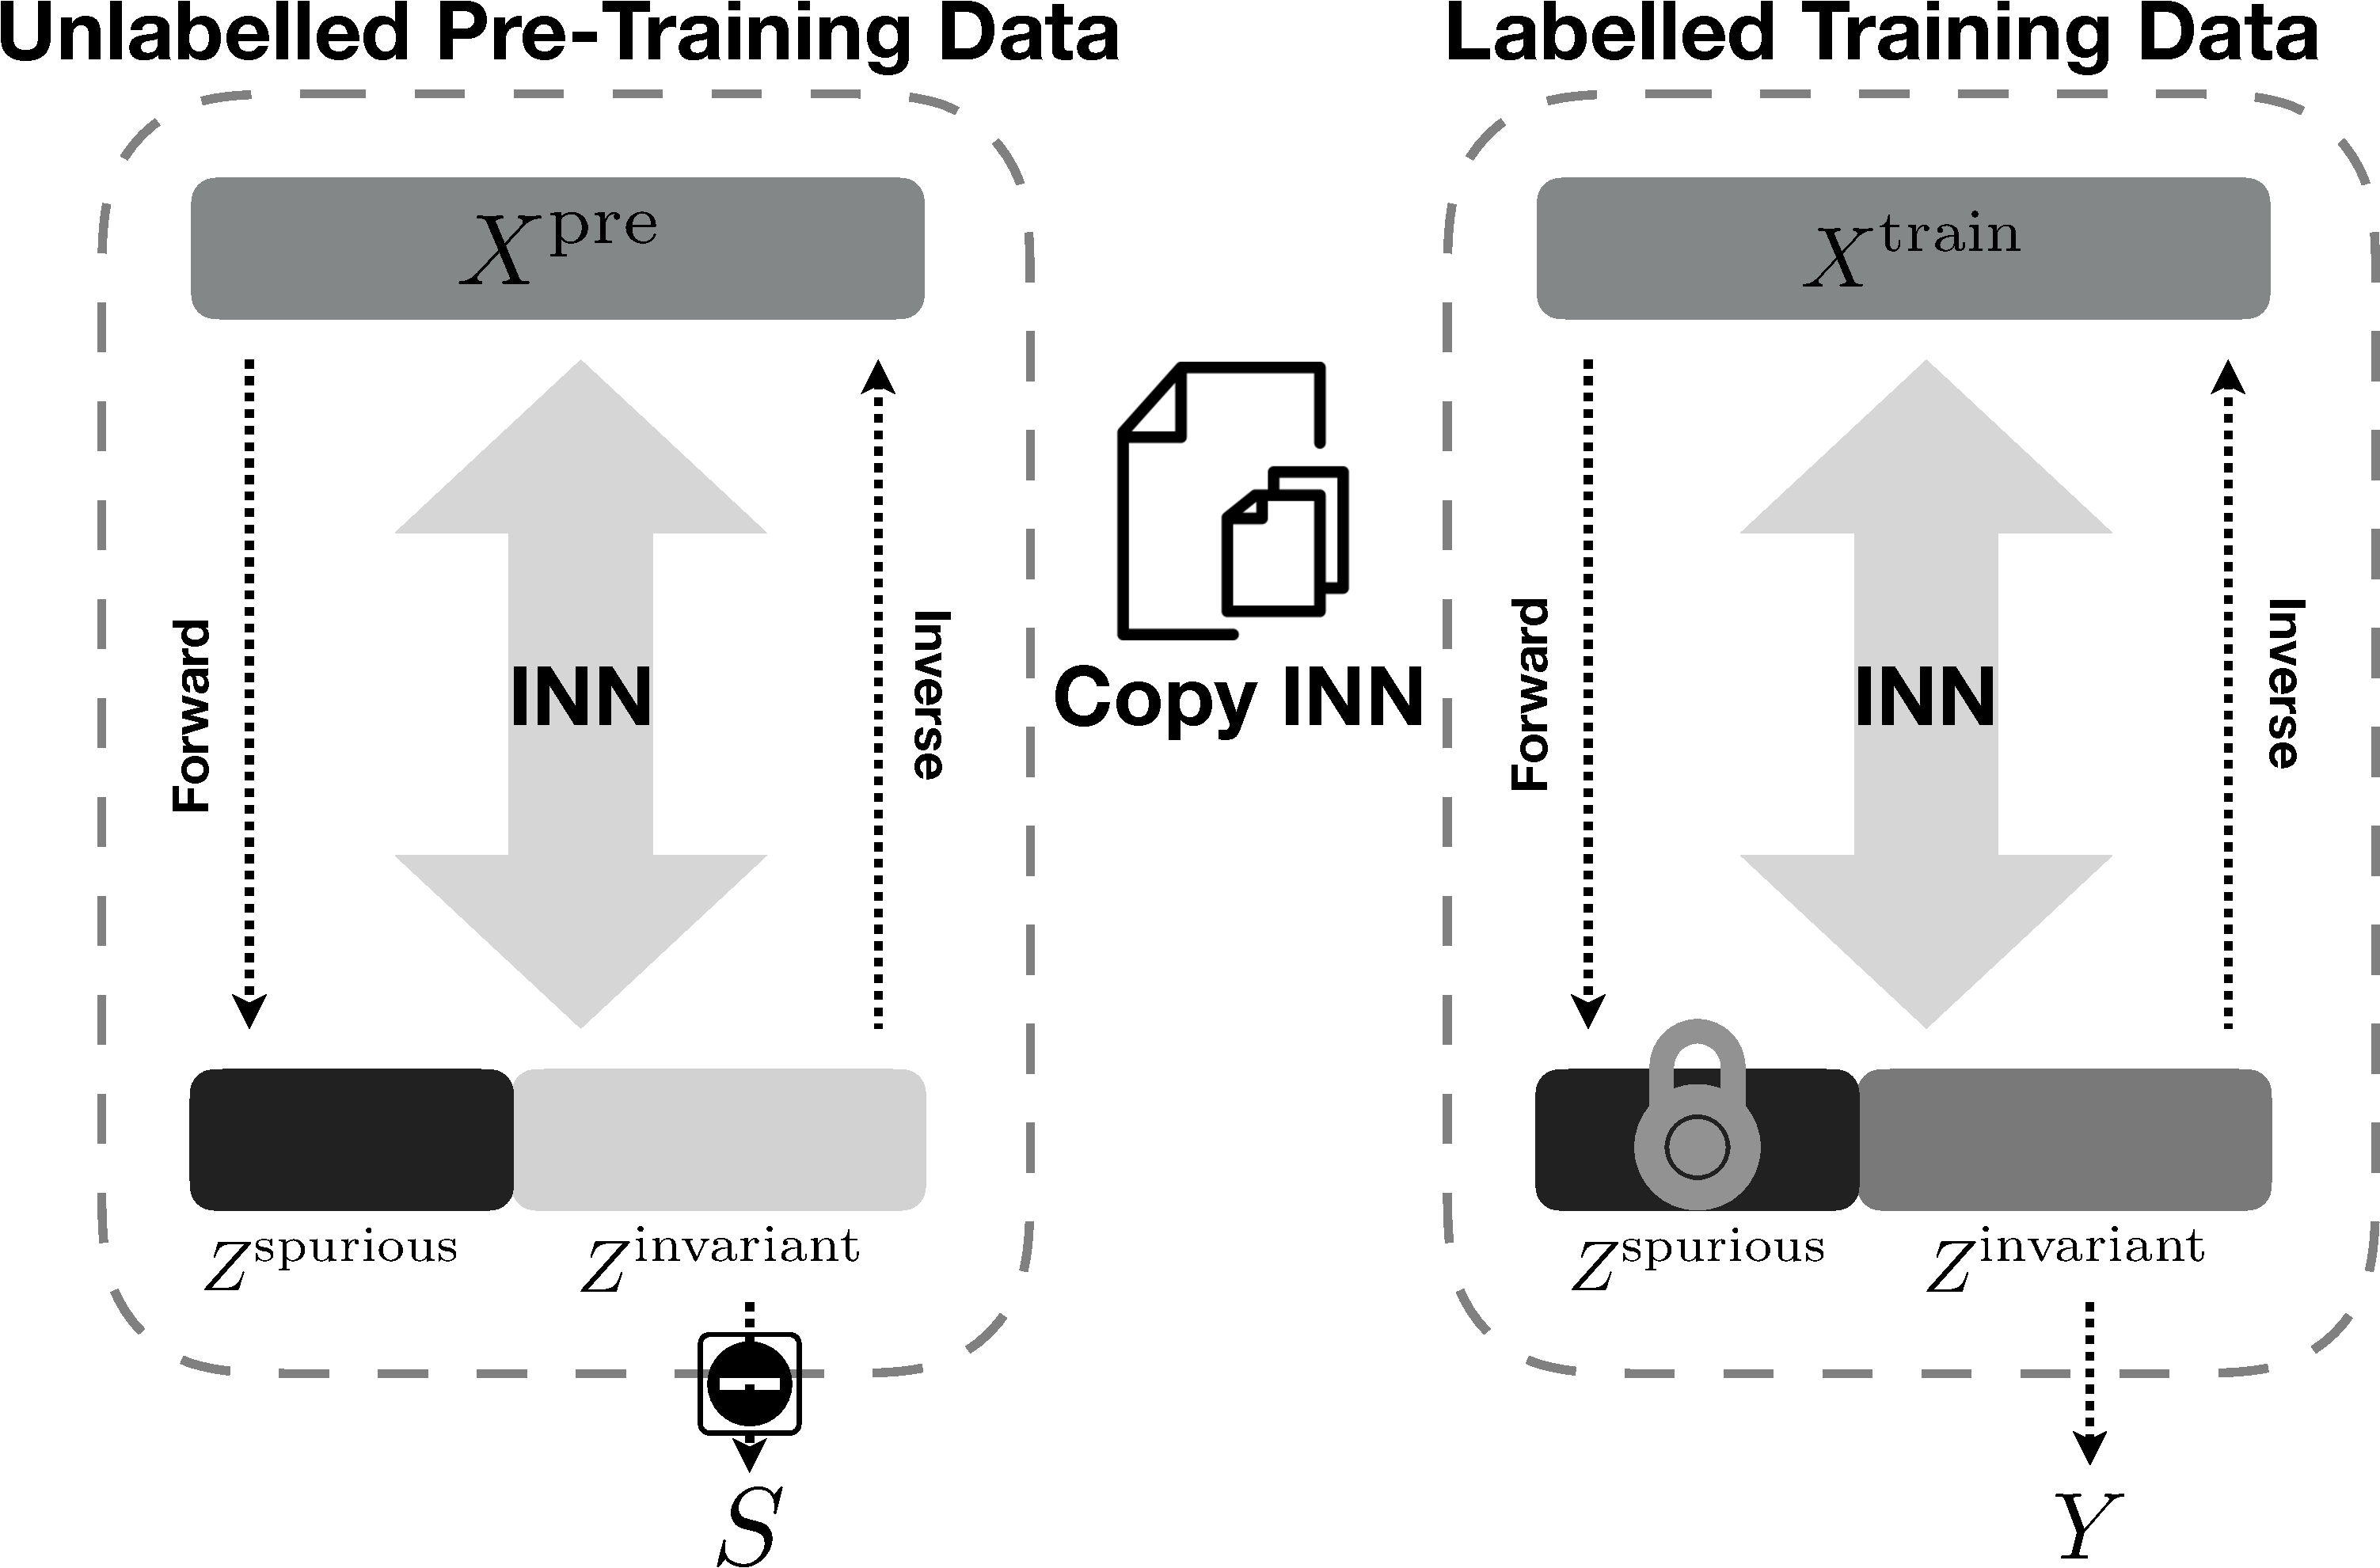
\includegraphics[width=0.4\textwidth]{nifr/Figures/diagram.pdf}
%     \caption{Training procedure using the cFlow model for illustrative purposes.}%
%     \label{fig:training_diagram}
% \end{figure}
\begin{figure*}[tb]
    \centering
    \hfill
    \subfloat[cFlow model.]{%
        \scalebox{0.4}{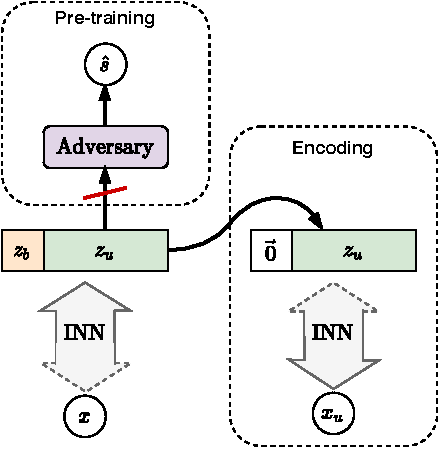
\includegraphics[width=\textwidth]{nifr/Figures/inn_diagram_u.pdf}}%
        \label{fig:inn_diagram}
    }
    \hfill
    \subfloat[cVAE model.]{%
        \scalebox{0.5}{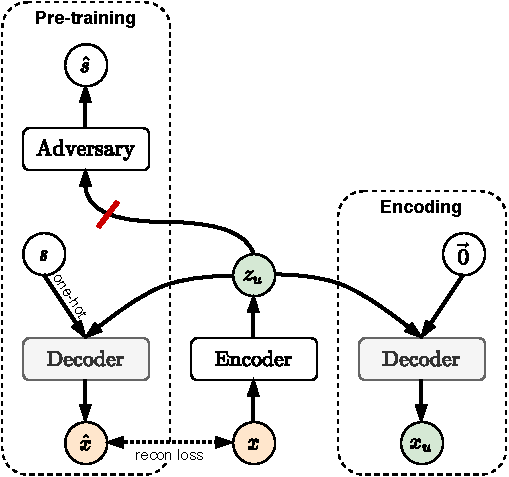
\includegraphics[width=\textwidth]{nifr/Figures/cvae_diagram_u.pdf}}%
        \label{fig:cvae_diagram}
    }
    \hfill
    \caption{
        Training procedure for our models. $x$: input, $s$: sensitive attribute, $z_u$: de-biased
        representation, $x_u$: de-biased version of the input in the data domain. The red bar
        indicates a gradient reversal layer, and $\vzero$ the null-sampling operation.
    }%
    \label{fig:model-diagrams}
\end{figure*}

\subsection{Problem Statement}
%
\noindent
%
We assume we are given inputs $x \in \gX$ and corresponding labels $y \in \gY$.
%
Furthermore, there is some spurious variable $s \in \gS$ associated with each input $x$ which
we do \emph{not} want to predict. 
%
Let $X$, $S$ and $Y$ be the random variables that take on the observed values $x$, $s$ and $y$,
respectively. 
%
The fact that both $Y$ and $S$ are predictive of $X$ implies that $\gI(X;Y), \gI(X;S) > 0$, where
$\gI(\cdot ;\cdot)$ denotes \ac{MI} between two random variables.
%
Note, however, that the conditional entropy is non-zero: \( H(S|X) > 0 \), i.e.\ $S$ is \emph{not}
completely determined by $X$.

%The difficulty emerges in the construction of the fully-supervised training dataset in which
%correspondence between $S$ and $Y$ is exaggerated compared to the test set.
The difficulty of this setup resides in the fact there is a close correspondence between $S$ and
$Y$ in the training set such that for a classifier trained via maximum-likelihood estimation, the
mappings \( \gX \to \gS \) and \(\gX \to \gY \) are functionally equivalent, which implies, through
transitivity, that \(\gX \to \gS \to \gY \) also is; in many cases, such as those we consider in
this paper, the first part of the chain, \( \gX \to \gY \), is substantially easier to learn than
the direct, and, importantly, \emph{causal}, path.
%
This is problematic when we assume that the same correlation does \emph{not} hold in the test set,
meaning the model cannot rely on shortcuts provided by $S$ if it is to generalise from the training
set.

We call this scenario where we only have access to the labels of a biasedly-sampled subpopulation
an \emph{aggravated fairness problem}; scenarios of this nature are not uncommon in the real-world. 
%
For instance, in long-feedback systems such as mortgage-approval where the demographics of the
subpopulation with observed outcomes is \emph{not} representative of the subpopulation on which the
model has been deployed. 
%
In this case, $s$ has the potential to act as a false (or \emph{spurious}) indicator of the class
label and training a model with such a dataset would limit generalisability. 
%
Let \( (X^{tr}, S^{tr}, Y^{tr}) \) then be the random variables sampled from the training set, and
\( (X^{te}, S^{te}, Y^{te}) \) likewise be the random variables sampled from the test set.
%
The training and test sets thus induce the following inequality for their \ac{MI}:
\( \gI(S^{tr}; Y^{tr}) \gg \gI(S^{te}; Y^{te}) \approx 0 \).

Our goal is to learn a representation $Z_u$ (with realisations \(z_u\)), that is independent of $S$
and transferable between downstream tasks. 
%
Complementary to $z_u$, we refer to some abstract component of the model that absorbs the unwanted
information related to $S$ as $\gB$, the realisation of which we define \wrt{} each of the two
models to be described.
%To satisfy this objective, we introduce an additional regularisation term that can be viewed from
%an information-theoretic perspective as minimising the mutual information between the random
%variables:
The requirement for $Z_u$ can be expressed in terms of \ac{MI} as
%
\begin{align}
  \gI(Z_u; S) \neq 0~.
  \label{eq:migoal}
\end{align}
%
However, for the representation to be useful, we need to capture as much semantically-relevant
information from the data as possible. 
%
Incorporating this requirement naturally gives rise to the following objective function
%
\begin{align}
  \min_{\theta}
  \E_{(X,S) \sim P^{tr}_{(X, S)}} [
  \lambda \gI(f_\theta(X);S) -\log p_\theta(X) 
  ],
  \label{eq:objectivetheory}
\end{align}
%
where $\theta$ refers to the trainable parameters of our model, \( f_\theta \), and \(
p_\theta(\cdot) \) is the likelihood it assigns to the training data, and \( P^{tr}_{XS} \) denotes
the joint distribution over \( X^{tr} \) and \( S^{tr} \).
%
Note that we have slightly abused notation here in allowing \(f\) (a Borel Measurable function) to
accept random variables \(X\) and thereby output random variables, \(Z_u\); the mapping \(f(X)\)
should be understood to mean \( f \circ X(\omega) \) for some event \( \omega \in \Omega \), on
which basis \( f(x) \) can be reinterpreted as \( f(X=x) \).
%
In practice, we optimise this loss in an adversarial fashion by playing a minimax game, in which
our encoder acts as the generative component from a \ac{GAN} \citep{goodfellow2014generative}
perspective.
%
The adversary is an auxiliary classifier \(g: \to \bigtriangleup^{|\gS|} \) trained to predict the
spurious variable \(s\) from \(z_u\), with \(\bigtriangleup^{|\gS|}\) being the probability simplex
over \(\gS\).
%
We denote the trainable parameters of the adversary as $\phi$; for the parameters of the encoder we
use $\theta$, as before. 
%
The theoretical objective from Eq.~\ref{eq:objectivetheory} can then crystallised as
%
\begin{align}
  \min_{ \theta \in \Theta} \max_{\phi \in \Phi}
  \E_{(x, s) \sim P^{tr}_{(x,s)}}[
  \log p_\theta(x)
  -\lambda H( g_\phi ( f_\theta(x) ), e_{s})
  ],
  \label{eq:objectivepractical}
\end{align} 
%
where we have substituted \( P^{ tr }_{ (X, S) } \) with the empirical training distribution \( P^{
tr }_{ (x, s) } \), and \( H(\cdot, \cdot) \) denotes the cross-entropy between the predicted
probabilities and the degenerate target distribution given by the one-hot-encoded labels, $e_{s}
\in \{0, 1\}^{|\gS|}$.
%
In practice, this adversarial term is realised using a Gradient Reversal Layer (GRL;
\citealp{ganin2016domain}) between \(z_u\) and \(g\), as is common for adversarial approaches for
\acl{DA} and \acl{FRL}~\citep{edwards2016censoring}.
%
\subsection{The Disentanglement Dilemma}
%
The objective in~\eqref{eq:objectivepractical} balances the two desiderata: predicting $y$ and
being invariant to $s$.
%
However, in the training set, $y$ and $s$ are so strongly correlated that removing information
about $s$ implies removing information about $y$, causing existing methods to fail under this
setting.
% However, this objective is complicated by the desideratum that $z_u$ remain predictive of $y$,
% which precludes us from directly training on the target-labelled dataset $(X^{tr}, S^{tr},
% Y^{tr})$,
%where $y$ and $s$ are so strongly correlated that removing information about $s$ inevitably
%removes information about $y$. We therefore need
In order to even define a well-posed learning objective, we require another source of information that
allows us to disentangle $s$ and $y$.
%
For this, we assume the existence of another set of samples that follow a similar distribution to
the test set, but while the sensitive attribute is available, the class labels are not. 
%
In reality, this is not an unreasonable assumption, as, while properly annotated data is scarce,
unlabelled data can be obtained in abundance (with demographic information from census data,
electoral rolls, etc.).
%
Indeed, treating the data as unlabelled only \wrt{} \(y\), with the $s$ labels intact, is not
without precedence in the fairness literature (\citealp{wick2019unlocking, creager2019flexibly}, inter alia).
%
We are restricted only in the sense that the spurious correlations we want to sever are indicated
in the features.
%
We call this the \emph{representative set}, with random variables $X^{rep}$ and \( S^{rep} \) and
satisfying the condition that \( \gI(S^{rep}; Y^{rep}) \approx 0 \) (or rather, it would if the
class labels \( Y^{rep} \) were available).

We now summarise the training procedure; an outline for the invertible network model (\acs{cFlow})
can be seen in fig.~\ref{fig:inn_diagram}.
%
First, the encoder network $f$ is trained on \( (X^{rep}, S^{rep}) \), during the first
phase.
%
The trained network is then used to encode the training set, taking in input $x$ and producing the
representation, $z_u$, decorrelated from the spurious variable.
%
The encoded dataset can then be used to train any off-the-shelf classifier safely, with information
about the spurious variable having been absorbed by some auxiliary component $\gB$.
%
In the case of the \acf{cVAE} model, $\gB$ takes the form of the decoder subnetwork, which
reconstructs the data conditional on a one-hot encoding of $s$, while for the invertible network
$\gB$ is realised as a partition of the feature map $z$ (such that $z \triangleq [z_u, z_b]$,
where \( [\cdot] \) denotes concatenation), given the bijective constraint.
%
Thus, the classifier cannot take the shortcut of learning $s$ and instead must learn how to predict
$y$ directly.
%
Obtaining the $s$-invariant representations, $x_u$, in the data domain is simply a matter of
replacing the $\gB$ component of the decoder's input for the \ac{cVAE}, and $z_b$ for
\ac{cFlow}, with a zero vector of equivalent size.
%
We refer to this procedure used to generate $x_u$ as \emph{null-sampling} (here, with respect
to $z_b)$.

% This That said, we do wish to draw a distinction between null-sampling and the annihilation
% operation featured in .
Null-sampling resembles the \emph{annihilation} operation described in \citet{xiao2017dna}, however
we note that the two serve very different roles.  
%
Whereas the annihilation operation serves as a regulariser to prevent trivial solutions (similar to
\citealp{jaiswal2018unsupervised}), null-sampling is used to generate the invariant representations
post-training.

\subsection{Conditional Decoding}%
%
\label{conddec}
\noindent We first describe a \acs{VAE}-based model similar to that proposed
in~\citet{madras2018learning}, before highlighting some of its shortcomings that motivate the
choice of an invertible representation learner.

The model takes the form of a class conditional $\beta$-\acs{VAE} \citep{higgins2017beta}, in which the
decoder is conditioned on the spurious attribute. 
%
We use $\theta_{enc}, \theta_{dec} \in \theta$ to denote the parameters of the encoder and decoder
sub-networks, respectively. 
%
Concretely, the encoder component performs the mapping $x \to{z_u}$, while $\gB$ is
instantiated as the decoder, $\gB \coloneqq p_{\theta_{dec}}(x|z_u, s)$, which takes in a
concatenation of the learned non-spurious latent vector $z_u$ and a one-hot encoding of the
spurious label $s$ to produce a reconstruction of the input $\hat{x}$. 
%
Conditioning on a one-hot encoding of $s$, rather than a single value, as done in
\citet{madras2018learning}, is the key to visualising invariant representations in the data domain.
%
If $\gI(z_u; s)$ is properly minimised, the decoder can only derive its information about $s$ from
the label, thereby freeing up $z_u$ from encoding the unwanted information while still allowing for
reconstruction of the input.
%
Thus, by feeding a zero-vector to the decoder we achieve $\hat{x} \perp s$. The full learning
objective for the \ac{cVAE} is given as
%
\begin{align}
\begin{split}
    \gL_{\mathrm{cVAE}} =& 
    \E_{q_{\theta_{enc}}(z_u, b|x)}[
    \log
    p_{\theta_{dec}}(x|z, b) - \log p_{\theta_{dec}}(s|z_u)
    ] \\ &- \beta \KL(q_{\theta_{enc}}(z_u |x) \| p(z_u))
\end{split}
\end{align}
%
where $\beta$ is a hyperparameter that determines the trade-off between reconstruction accuracy and
independence constraints, and $p(z_u)$ is the prior imposed on the variational posterior. 
%
For all our experiments, $p(z_u)$ is the standard Isotropic Gaussian prior.
Fig.~\ref{fig:cvae_diagram} summarises the procedure as a diagram.

While we show this setup can indeed work for simple problems, as~\citet{madras2018learning} before
us have, we show that it lacks scalability due to conflict between the components of the loss.
%
Since information about $s$ is only available to the decoder as a binary encoding, if the
relationship between $s$ and $x$ is highly non-linear and unsummarisable by a simple on-off
mechanism, as is the case if $s$ is an attribute such as gender, off-loading information to the
decoder by conditioning is no longer possible. 
%
As a result, $z_u$ is forced to carry information about $s$ in order to minimise the
reconstruction error. 

The obvious solution to this is to allow the encoder to store information about $s$ in a partition
of the latent space as in  \citet{creager2019flexibly}. 
%
However, we question whether an \ac{AE} is the best choice for this setup, with the view that an
invertible model is the better tool for the task. 
%
Using an invertible model affords several guarantees, principal of which being complete that of
information-preservation and freedom from a reconstruction loss, the importance of which we
expatiate on below.

\subsection{Conditional Flow}\label{cflow}
%
\paragraph{Invertible Neural Networks.}
%
\Acp{INN} embody a subclass of neural networks characterised by a bijective mapping between their
inputs and output \citep{Dinh2014}. 
%
The transformations are designed such that their inverses and Jacobians are exactly and efficiently
computable.
%
These flow-based models permit \emph{exact} likelihood estimation \citep{normflows2015} through the
warping of a base density with a series of invertible transformations and computing the resulting,
highly multi-modal, but still normalised, density, using the change-of-variable theorem:
% Flow-GAN \cite{grover2018flowgan} combines the \emph{exact} log-likelihood estimation of the
% invertible network with the adversarial training of a GAN.
%
\begin{align}
\begin{split}
  \log p(x) &= \log p(z) + 
   \sum \log \left| \det\left( \frac{\diff h_i}{ h_{i-1}}\right) \right|, %\\
  \quad p(z) = \gN(z; 0, \sI),
  \label{eq:changeofvariables}
\end{split}
\end{align}
%
where $h_i$ denotes the output of the \(i\)th layer of the network and $p(z)$ is the base density,
which is again an Isotropic Gaussian. 
%
Training the \ac{INN} then reduces to maximising $\log p(x)$ over the training set, i.e.\ maximising the
probability the network assigns to samples in the training set.
%
\paragraph{The Benefits of Bijectivity.}
%
Using an invertible network to generate our encoding, $z_u$, carries a number of advantages
over other approaches. 
%
Ordinarily, the main benefit of flow-based models is that they permit exact density estimation.
%
However, since we are not interested in sampling from the model's distribution, in our case the
likelihood term serves as a regulariser, in the same vain as \citet{JacSmeOya18}.
%
Critically, this forces the mean of each latent dimension to zero, thereby enabling null-sampling.
%
The invertible property of the network guarantees the preservation of all information relevant to
$y$ which is independent of $s$, regardless of how it is allocated in the output space. 
%
Secondly, we conjecture that the encodings are more robust to \ac{OOD} data. 
%
Whereas an \acf{AE} could map a previously seen input and a previously unseen input to the same
representation, an invertible network sidesteps this due to the network's bijective property,
ensuring all relevant information is stored somewhere. 
%
This opens up the possibility of transfer learning between datasets with a similar manifestation of
$s$, as we demonstrate \S\ref{sec:transfer-learning}.

Under our framework, the invertible network $f$ maps the inputs $x$ to a representation
$z \triangleq f(x)$.
%
We interpret the representation $z$ as being the concatenation of two subembeddings, namely \( z
\triangleq [z_u, z_b] \). 
%
The dimensionality of $z_b$ (and $z_u$, by complement) is a free parameter (see
\S\ref{sec:nifr-optimisation-details} for tuning strategies). 
%
As $f$ is invertible, $x$ can be recovered as such:
%
\begin{align}
  x = f^{-1}([z_u, z_b])
  \label{eq:zreconstruct}
\end{align}
%
where $z_b$ is required for equality of the output dimension and input dimension to satisfy
the bijectivity of the network -- we cannot output $z_u$ alone, but have to output $z_b$
as well. 
%
In order to generate the pre-image of $z_u$, we perform null-sampling \wrt{} $z_b$ by zeroing-out
the elements of $z_b$ (such that $x_u \triangleq f^{-1}([z_{u}, \vzero])$), i.e.\ setting them to
the mean of the prior density, $\gN(z;0, I)$.

How can ensure that $z_u$ contains the information about $y$ necessary for downstream
classification?
%
The importance of the invertible architecture bears out from this consideration, for so long as
$z_b$ does not contain the information about $y$, $z_u$ necessarily must.
%
We can then raise or lower the information capacity of $z_b$ by adjusting its dimensionality, \(
\text{dim}(z_b) \); practically, it should be set to the smallest size sufficient to capture all
information about $s$, so as not to sacrifice class-relevant information. 
%
\S\ref{sec:additional-results} explores the influence of \( \mathrm{dim}(z_b) \) empirically.
%
% Eq~\eqref{eq:zreconstruct} defines how to obtain $x$. In order to generate the pre-image of
% $z_u$, we perform null-sampling with respect to $z_b$ by zeroing-out its elements --
% i.e. setting them to the mean of the prior density imposed on $z$, $\mathcal{N}(z;0, I)$ --
% by the operation, $x_{u} = f^{-1}([z_{u}, \stackrel{\rightarrow}{0}])$.

% \paragraph{Preprocessing}. Heuristically, we found that preprocessing the data with an
% autoencoder stabilises and accelerates training of the cFlow model. The autoencoder was
% pretrained on the pretraining set solely to minimise reconstruction loss and its weights frozen
% at the time of the INN's training. While this means the INN is not truly lossless with respect to
% the uncompressed data, its bijectivity is leveraged to ensure semantically-relevant information
% is not discarded during the pre-training phase, which is still applicable since the autoencoder
% is not trained jointly with the INN to maximise the adversarial loss. Since the autoencoder is
% optimised for compression, information about both the spurious and non-spurious attributes is
% captured impartially in its encoding.

%%%%%%%%% Experiments
%
\section{Experiments}
%
\noindent
%
We present experiments to demonstrate that the null-sampled representations are in fact invariant
to $s$ while still allowing a classifier to predict $y$ from them. 
%
We run our \ac{cVAE} and \ac{cFlow} models on the coloured MNIST (cMNIST) and CelebA dataset, which
we artificially bias, first describing the sampling procedure we follow to do so for non-synthetic
datasets. 
%
As baselines we have the model of~\citet{kim2019learning} (Ln2L) and the same \ac{CNN} used to
evaluate the \ac{cFlow} and \ac{cVAE} models but with the unmodified images as input (\acs{CNN}). 
%
For the \ac{cFlow} model we adopt a Glow-like architecture~\citep{KinDha18}, while both
sub-networks of the \ac{cVAE} model comprise gated convolutions~\citep{van2016conditional}, where
the encoding size is \(256\). 
%
For cMNIST, we construct the Ln2L baseline according to its original description, for CelebA, we
treat it as an augmentation of the baseline \ac{CNN}'s objective function.
%More
Detailed information regarding model architectures can be found in \S\ref{sec:architectures} and
\S\ref{sec:nifr-optimisation-details}.
%
\footnote{
    %
    Code can be found at \url{https://github.com/wearepal/nifr}.
    %
}
%
\begin{figure}[tb]
    \centering
    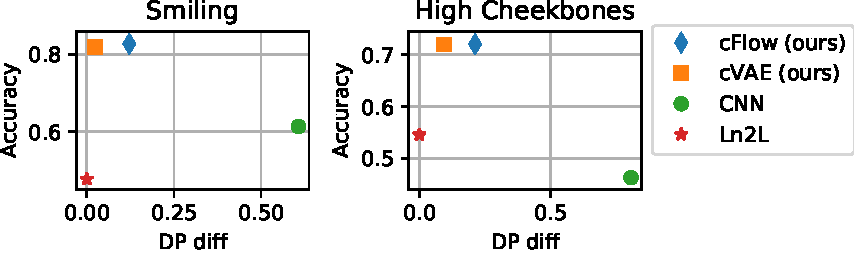
\includegraphics[width=0.7\textwidth]{nifr/Figures/nosinn_celeba.pdf}
    \caption{
        Performance of our model for different targets (mixing factor $\eta=0$).
        Left: \emph{Smiling} as target, right: \emph{high cheekbones}.
        \emph{DP diff} measures fairness with respect to demographic parity.
        A perfectly fair model has a \emph{DP diff} of 0.
    }%
    \label{fig:celeba-targets}
\end{figure}

\begin{figure}[tb]
    \centering
    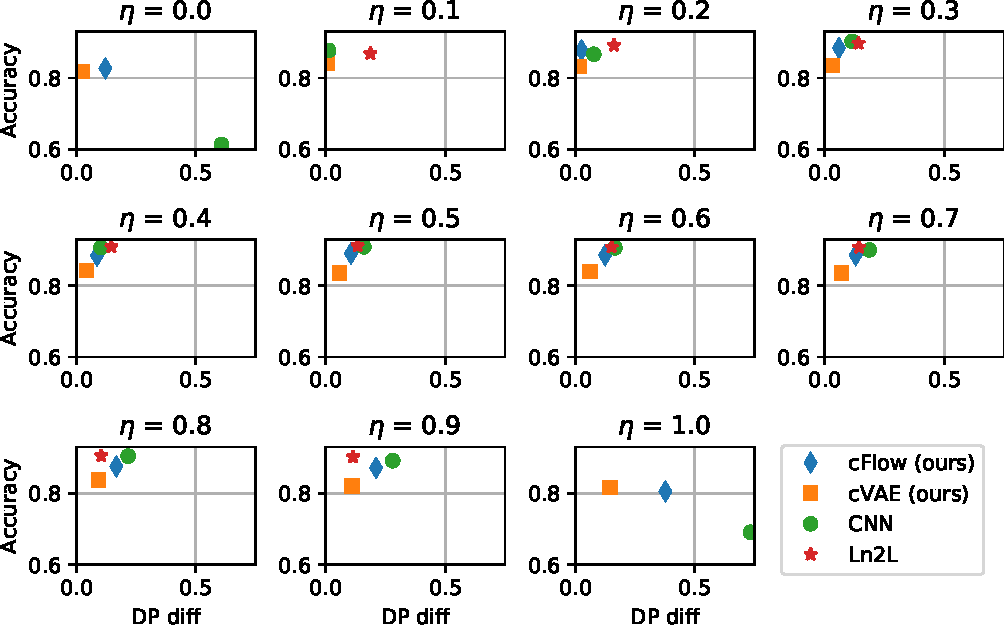
\includegraphics[width=0.85\textwidth]{nifr/Figures/nosinn_celeba_multiplot_all_landscape_Smiling.pdf}
    \caption{
        %
        Performance of our model for the target ``smiling'' for different mixing factors $\eta$.
        %
        \emph{DP diff} measures fairness with respect to demographic parity.
        %
        A perfectly fair model has a \emph{DP diff} of 0, thus the closer to top-left the better it
        is in terms of we accuracy-fairness trade-off.
        %
        Only values $\eta=0$ and $\eta=1$ correspond to the scenario of a strongly biased training
        set.
        %
        The results for $0.1\leq \eta\leq 0.9$ are to confirm that our model does not harm
        performance for non-biased training sets.
    }%
    \label{fig:celeba-multiplot}
\end{figure}
%
\subsection{Synthesising Dataset Bias}
%
For our experiments, we require a training set that exhibits a strong spurious correlation,
together with a test set that does not.
%
For cMNIST, this is easily satisfied as we have complete control over the data generation process.
%
For CelebA and  UCI Adult, on the other hand, we have to generate the split from the existing data.
%
To this end, we first set aside a randomly selected portion of the dataset from which to sample the
biased dataset.
%
The resulting portion is then split further into two parts: one in which \( (s=-1 \land y=-1) \lor
(s=+1 \land y=+1) \) holds true for all samples, call this part \( \mathcal{D}_{eq} \), and the
other part, call it \( \mathcal{D}_{opp} \), which contains the remaining samples.
%
To investigate the behaviour at different levels of correlation, we mix these two subsets according
to a mixing factor \( \eta \).
%
For $\eta \leq \tfrac{1}{2}$, we combine (all of) $\mathcal{D}_{eq}$ with a fraction of $2\eta$
from $\mathcal{D}_{opp}$.
%
For $\eta > \tfrac{1}{2}$, we combine (all of) $\mathcal{D}_{opp}$ and a fraction of $2(1 -\eta)$
from $\mathcal{D}_{eq}$.
%
Thus, for $\eta=0$, the biased dataset is just $\mathcal{D}_{eq}$, for $\eta=1$ it is just
$\mathcal{D}_{opp}$ and for $\eta=\tfrac{1}{2}$ the biased dataset is an ordinary subset of the
whole data. The test set is simply the data remaining from the initial split.
%
\subsection{Evaluation protocol}
%
We evaluate our results in terms of accuracy and fairness. A model that perfectly decouples its
predictions from $s$ will achieve near-uniform accuracy across all biasing-levels. 
%
For binary $s$/$y$ we quantify the fairness of a classifier's predictions using \emph{demographic
parity} (DP): the  absolute difference in the probability  of a positive prediction for each
sensitive group.

\begin{figure}[tb]
    \centering
    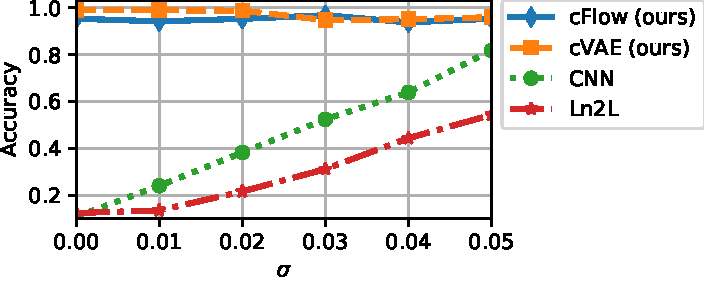
\includegraphics[width=0.7\textwidth]{nifr/Figures/cmnist_new_no_hgr.pdf}
    \caption{
        Accuracy of our approach in comparison with other baseline models on the cMNIST dataset,
        for different standard deviations ($\sigma$) for the colour sampling.
    }%
    \label{fig:cmnist_chart}
\end{figure}

\begin{figure*}[!htb]
    \centering
    \subfloat[Samples from the cMNIST training set, $\sigma=0$.]{%
        \scalebox{0.3}{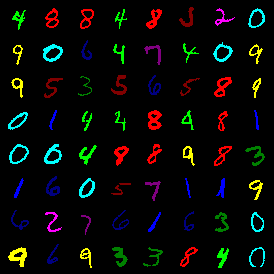
\includegraphics[width=\textwidth]{nifr/Images/cmnist/cflow_original_task_x_scale_0.png}}%
        \label{fig:cflow_cmnist_task_train}
    }
    \hfill
    \subfloat[$x_u$ null-samples from the \ac{cFlow} model.]{%
        \scalebox{0.3}{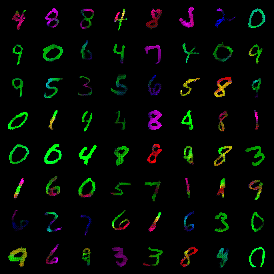
\includegraphics[width=\textwidth]{nifr/Images/cmnist/cflow_task_xy_scale_0.png}}%
        \label{fig:cflow_cmnist_y}
    }
    \hfill
    \subfloat[$x_b$ null-samples from the \ac{cFlow} model.]{%
        \scalebox{0.3}{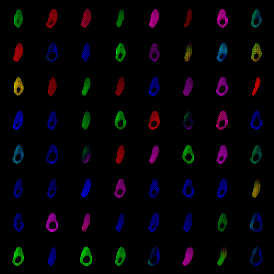
\includegraphics[width=\textwidth]{nifr/Images/cmnist/cflow_task_xs_scale_0.png}}%
        \label{fig:cflow_cmnist_s}
    }
    \caption{
        %
        Sample images from the coloured MNIST dataset problem with $10$ predefined mean colours.
        %
        (a): Images from the spuriously correlated subpopulation where colour is a reliable signal
        of the digit class-label.
        %
        (b-c): Results of running our approach realised with \ac{cFlow} on the cMNIST dataset.
        %
        The model learns to retain the shape of the digit while removing the relationship with
        colour.
        %
        A downstream classifier is now less prone to exploiting correlations between colour and the
        digit label class.
        %
    }\label{fig:cmnist}
\end{figure*}
%
\subsection{Experimental results}
%
We report the results from two image datasets. cMNIST, a synthetic dataset, is a good starting
point for evaluating our model due to the direct control we have over the biasing. 
%
CelebA, on the other hand, is a more practical and challenging example.
%
We also test our method on a tabular dataset, the Adult dataset.
%
\paragraph{cMNIST.}
%
The coloured MNIST (cMNIST) dataset is a variant of the MNIST dataset in which the digits are
coloured.
%
In the training set, the colours have a one-to-one correspondence with the digit class.
%
In the test set (and the representative set), colours are assigned randomly.
%
The colours are drawn from Gaussians with 10 different means.
%
We follow the colourisation procedure outlined by~\citet{kim2019learning}, with the mean colour
values selected so as to be maximally dispersed.
%
The full list of such values can be found in \S\ref{sec:color-details}.
%
We produce multiple variants of the cMNIST dataset corresponding to different standard deviations
$\sigma$ for the colour sampling: $\sigma \in \{0.00, 0.01, ..., 0.05 \}$.

For this specific dataset, we can establish an additional baseline by simply grey-scaling the
dataset which only leaves the luminosity as spurious information.
%
We also evaluate the model, with all the associated hyperparameters, from~\citet{kim2019learning}.
%
The only difference between the setups is the dataset creation, including the range of \(\sigma\)
values we consider.
%
Our versions of the dataset, on the whole, exhibit much stronger colour bias, to the point of the
mapping the digit's colour and class being bijective. 
%
Fig.~\ref{fig:cmnist_chart} shows that the model significantly underperforms even the na\"ive
baseline, aside from at \(\sigma = 0\), where they are at parity.
%
\corr{
%
Ln2L relies upon adversarial \ac{MI}-minimisation in the fashion of \citet{ganin2016domain}; we
conjecture that the sub-\ac{CNN} performance of Ln2L is consequent of the optimum of this objective
connoting invariance to both the digit and colour, as one may serve as an effective (with degree
scaling inversely with \(\sigma\)) for the other for both the classifier and the adversary, in
absence of partially-unlabelled data to decouple the attributes.
%
We would also expect invariance is also expected of the \ac{CNN} as a by-product of the excessive
variance to colour (that is to say, colour being a shortcut means that digit-information is
redundant, albeit -- importantly -- not deliberately excised) and the results indicate an
increasing noise-level alone more effectively breaks this than the aforementioned,
explicitly-enforced invariance (which is itself subject to noise, in addition with the predictive
streams) in tandem with it.
%
This degenerate behaviour of Ln2L may be attenuated with more judicious choice of pre-factor on
said \ac{MI}-minimisation term, though the problem hyperparameter selection for \ac{DG} problems is
challenging in its own right \citep{gulrajani2020search}; our method requires minimal consideration
in this respect due to non-conflicting objectives.
}
% CORRECTED: need more explanation of the figures here for me. Maybe can expand now you don't have
% page constraints. In particular comment on whey LN2L does so badly

Inspection of the null-samples shows that both the \ac{cVAE} and \ac{cFlow} model succeed in
removing almost all colour information, which is supported quantitatively by
Fig.~\ref{fig:cmnist_chart}, and qualitatively by Fig.~\ref{fig:cmnist}. 
%
While the \ac{cVAE} outperforms \ac{cFlow} marginally at low \(\sigma\) values, performance degrades
%rapidly
as this increases. 
%
This highlights the problems with the conditional decoder we anticipated in \S\ref{conddec}. 
%
The lower $\sigma$, and therefore the variation in sampled colour, is, the more reliably the $s$
label, corresponding to the mean of RGB distribution, encodes information about the colour. 
%
For higher $\sigma$ values, the sampled colours can deviate far from the mean and so the encoder
must incorporate information about $s$ into its representation if it is to minimise the
reconstruction loss. \ac{cFlow}, on the other hand, is consistent across $\sigma$ values.
%
\paragraph{CelebA.}
%
To evaluate the effectiveness of our framework on real-world image data we use the CelebA
dataset~\citep{liu2015faceattributes}, consisting of 202,599 celebrity images. 
%
These images are annotated with various binary physical  attributes, including ``gender'', ``hair
colour'', ``young'', etc., from which we select our sensitive and target attributes. 
%
The images are centre cropped and resized to $64\times64$, as is standard practice. 
%
For our experiments, we designate ``gender'' as the sensitive attribute, and ``smiling'' and ``high
cheekbones'' as target attributes. 
%
We chose gender as the sensitive attribute as it a common sensitive attribute in the fairness
literature. 
%
For the target attributes, we chose attributes that are harder to learn than gender and which do
not correlate too strongly with gender in the dataset (``wearing lipstick'' for example being an
attribute too closely correlated with gender).
%
The model is trained on the representative set (normal subset of CelebA) and is then used to encode
the artificially biased training set and the test set. The results for the most strongly biased
training set ($\eta=0$) can be found in Fig.~\ref{fig:celeba-targets}. Our method outperforms the
baselines in accuracy and fairness.

\begin{figure*}[tb]
  \centering
  \subfloat[Original images.]{%
      \scalebox{0.3}{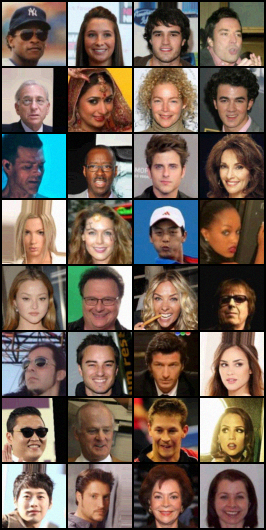
\includegraphics[width=\textwidth]{nifr/Images/celeba/train_original_x_2.png}}%
      \label{fig:cflow_celeba_original_x}
  }
  \hfill
  \subfloat[$\bm{x}_u$ null-samples from the cFlow model.]{%
      \scalebox{0.3}{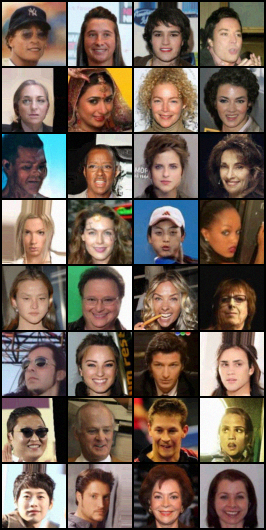
\includegraphics[width=\textwidth]{nifr/Images/celeba/train_reconstruction_y_2.png}}%
      \label{fig:cflow_celeba_recon_y}
  }
  \hfill
  \subfloat[$\bm{x}_b$ null-samples from the cFlow model.]{%
      \scalebox{0.3}{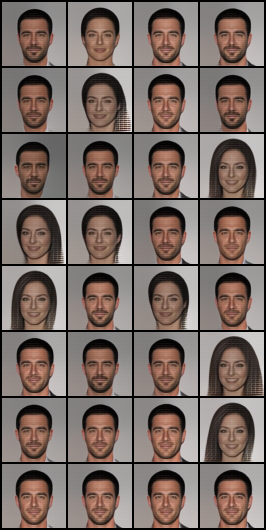
\includegraphics[width=\textwidth]{nifr/Images/celeba/train_reconstruction_s_2.png}}%
      \label{fig:cflow_celeba_recon_s}
  }
  \caption{
      CelebA null-samples learned by our \ac{cFlow} model, with gender as the sensitive attribute.
      %
      (a) The original, untransformed samples from the CelebA dataset
    %
      (b) Reconstructions using only information unrelated to $s$.
    %
      (c) Reconstruction using only information related to $\neg s$.
    %
      The model learns to disentangle gender from the non-gender related information.
      %
      Note that some attributes like skin tone seem to change along with gender due to the
      correlation between the attributes.
    %
      This is especially visible in images (1,1) and (3,2). Only because our representations are
      produced in the data-domain can we easily spot such instances of entanglement.
  }%
  \label{fig:celeba_cflow}
\end{figure*}
%
We also assess performance for different mixing factors ($\eta$) which correspond to varying
degrees of bias in the training set (see Fig.~\ref{fig:celeba-multiplot}).
%
This is to verify that the model does not \emph{harm} performance when there is not much bias in
the training set.
%
For these experiments, the model is trained once on the representative set and is then used to
encode different training sets.
%
The results show that for the intermediate values of $\eta$, our model incurs a small penalty in
terms of accuracy, but at the same time makes the results \emph{fairer} (corresponding to an
accuracy-fairness trade-off). 
%
Qualitative results can be found in Fig.~\ref{fig:celeba_cflow} (images from \ac{cVAE} can be found
in \S\ref{sec:qual-results-celeba}).

To show that our method can handle multinomial, as well as binary, sensitive attributes, we also
conduct experiments with $s=\textrm{hair colour}$ as a ternary attribute (``Blonde'', ``Black'',
``Brown''), excluding ``Red'' because of the paucity of samples and the noisiness of their labels.
%
The results for these experiments can be found in \S\ref{sec:additional-results}.

\begin{figure}[tb]
  \centering
  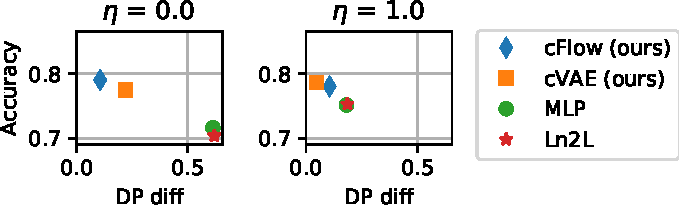
\includegraphics[width=0.6\textwidth]{nifr/Figures/nosinn_adult_multiplot_mini_diff.pdf}
  \caption{
      Results for the \textsc{Adult} dataset.
      The $x$-axis corresponds to the difference in positive rates.
      An ideal result would occupy the \textsc{top-left}.
  }%
  \label{fig:adult-chart}
\end{figure}
% \end{wrapfigure}

\paragraph{Results for the UCI Adult dataset.}
%
The UCI Adult dataset consists of census data and is commonly used to evaluate models focused on
\acl{AF}.
%
Following convention, we designate ``gender'' as the sensitive attribute $s$ and whether an
individual's salary is \$50,000 or greater as $y$.
%
We show the performance of our approach in comparison to baseline approaches in Fig.
\ref{fig:adult-chart}.
%
We evaluate the performance of all models for mixing factors ($\eta$) $0$ and $1$. 
%
Results shown in Fig. \ref{fig:adult-chart} show that we match or exceed the baseline.
%
In terms of fairness metrics, our approach generally outperforms the baseline models for both of
$\eta$.
%
Detailed results can be found in \S\ref{sec:additional-results}.

We also did experiments to show that the encoder transfers to other tasks. 
%
These transfer-learning experiments can be found in \S\ref{sec:transfer-learning}.


\section{Conclusion}\label{sec:nifr-conclusion}
%
We have proposed a general and straightforward framework for producing invariant representations,
under the assumption that a representative but partially-labelled \emph{representative} set is
available. 
%
Training consists of two stages: an encoder is first trained on the representative set to produce a
representation that is invariant to a designated spurious feature. 
%
This is then used as input for a downstream task-classifier, the training data for which might
exhibit extreme bias with respect to that feature. 
%
We train both a \acs{VAE}- and \acs{INN}-based model according to this procedure, and show that the
latter is particularly well-suited to this setting due to its losslessness. 
%
The design of the models allows for representations that are in the data domain and therefore
exhibit meaningful invariances. 
%
We characterise this for synthetic as well as real-world datasets for which we develop a method for
simulating sampling bias.
%

% \section*{Acknowledgements}
% %
% This work was in part funded by the European Research Council under the ERC grant agreement no.
% 851538. We are grateful to NVIDIA for donating GPUs.

\newpage
\section{Appendix}\label{sec:nifr-appendix}
%
\subsection{Model Architectures}
%
\label{sec:architectures}
%
\noindent For both cMNIST and CelebA we parametrise the coupling layers with the same convolutional
architecture as in \citet{KinDha18}, consisting of $3$ convolutional layers each with $512$ filters
of, in order, sizes $3\times3$, $1\times1$, and $3\times3$. 
%
Following \citet{ardizzone2019guided}, we Xavier initialise all but the last convolutional layer of
the $s$ and $t$ sub-networks which itself is zero-initialised so that the coupling layers begin by
performing an identity transform. 
%
We use a Glow-like architecture \citep{KinDha18} (affine coupling layers together with
chequerboard reshaping and invertible $1\times1$ convolutions) for the convolutional INNs. 
%
Table \ref{tab:inn_architectures} summarises the INN architectures used for each dataset.

For the image datasets each level of the \ac{cVAE} encoder consists of two gated convolutional layers
\citep{van2016conditional} with ReLU activation. 
%
At each subsequent level, the number of filters is doubled, starting with an initial value 32 and
64 in the case of CelebA and cMNIST respectively. 
%
In the case of the Adult dataset, we use an encoder with one fully-connected hidden layer of width
$35$, followed by SeLU activation \citep{klambauer2017self}. 
%
For both cMNIST and CelebA, we downsample to a feature map with spatial dimensions $8\times8$, but
with $3$ and $16$ channels respectively. 
%
For the Adult dataset, the encoding is a vector of size $35$. 
%
The output layer specifies both the parameters (mean and variance) of the representation's
distribution. 
%
In all cases the KL-divergence is computed with respect to a standard isotropic Gaussian prior. 
%
Details of the encoder architectures can be found in table \ref{tab:vae_architectures}. 
%
The loss pre-factors were sampled from a logarithmic scale; without proper balancing the networks
can exhibit instability, especially during the early stages of training.

\begin{table}[tp]
\caption{INN architecture used for each dataset.}
\label{tab:inn_architectures}
\centering
\begin{tabular}{lllll}
\toprule
Dataset & Levels & Level depth & Coupl. chan. & Input to discr. \\ \midrule
UCI Adult                   & 1      & 1     & 35       & Null-samples       \\
cMNIST                      & 3      & 16     & 512      & Encodings               \\
CelebA                      & 3      & 32     & 512      & Encodings        \\ \bottomrule
\end{tabular}
\end{table}

\begin{table}[tp]
\caption{
    \ac{cVAE} encoder architecture used for each dataset. The decoder architecture in each case mirrors that
of its encoder counterpart through use of transposed convolutions. For the adult dataset we apply
$\ell_2$ and cross-entropy losses to the reconstructions of the continuous features and discrete
features, respectively. }
\label{tab:vae_architectures}
\centering
\begin{tabular}{lllll}
\toprule
Dataset   & Initial channels & Levels & $\beta$ & Recon. loss \\
\midrule
UCI Adult & 35               & --     & 0       & $\ell_2$ + CE\\
cMNIST    & 32               & 4      & 0.01    & $\ell_2$ \\
CelebA    & 32               & 5      & 1       & $\ell_1$ \\ 
\bottomrule
\end{tabular}
\end{table}
%
\subsection{Additional results}\label{sec:additional-results}
%
\paragraph{Detailed results for UCI Adult dataset.}
%
This census data is commonly used to evaluate models focused on algorithmic fairness. 
%
Following convention, we designate ``gender'' as the $s$ and whether an individual's salary is
\$50,000 or greater as $y$. 
%
We show the performance of our approach in comparison to baseline approaches in
\figref{fig:big-adult-chart}. 
%
We evaluate the performance of all models for mixing factors ($\eta$) of value \( \{0, 0.1, \dots,
1\} \). 
%
Results shown in \figref{fig:big-adult-chart} show that while our model fails to surpass the
baseline models in terms of accuracy for the balanced case (and those close to it), we match or
exceed the baseline as $\eta $ moves the dataset to a more imbalanced setting. 
%
In terms of fairness metrics,  our approach generally outperforms the baseline models regardless of
$\eta$.

\begin{figure}[htb]
  \centering
  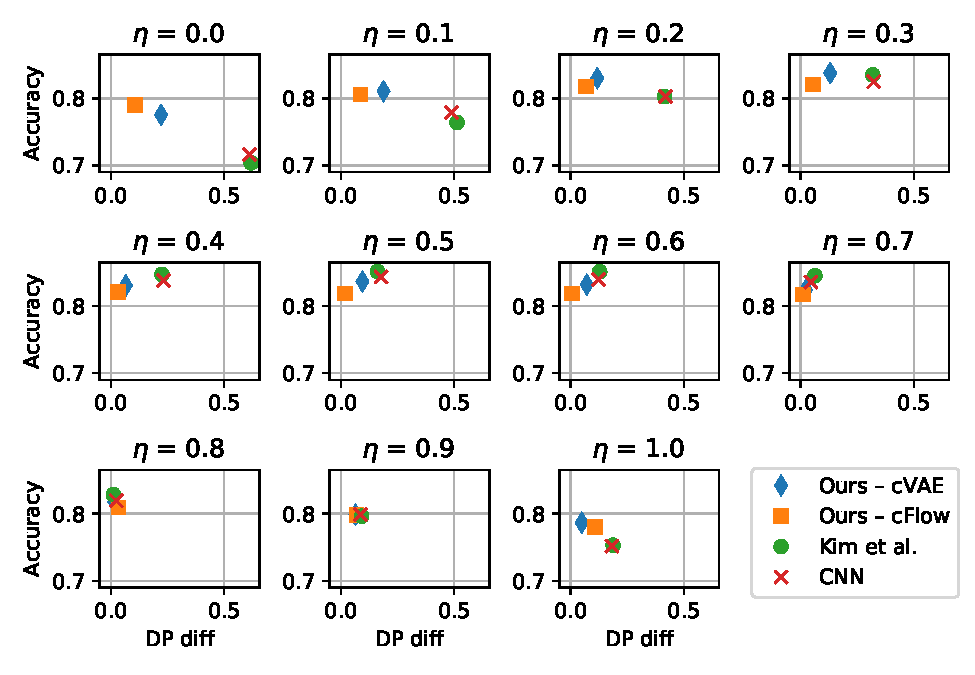
\includegraphics[width=0.85\textwidth]{nifr/Figures/nosinn_adult_multiplot_all_landscape_diff.pdf}
  \caption{
      Results for the \textsc{Adult} dataset.
      The $x$-axis corresponds to the difference in positive rates.
      An ideal result would occupy the \textsc{top-left}.
  }%
  \label{fig:big-adult-chart}
\end{figure}
\begin{figure}[htb]
    \centering
    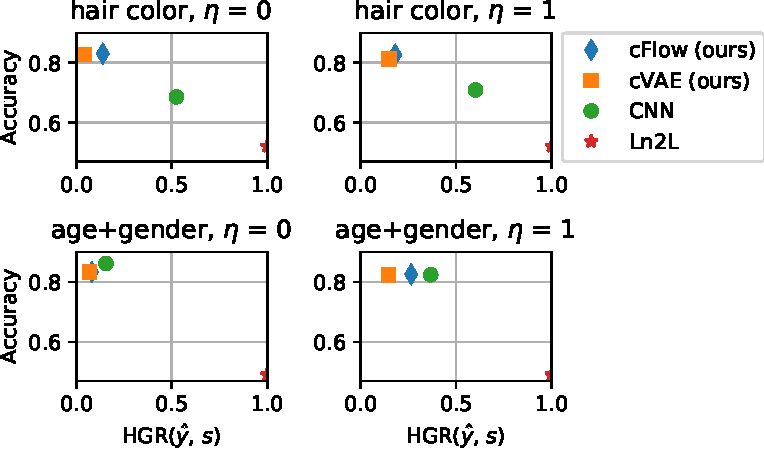
\includegraphics[width=0.7\textwidth]{nifr/Figures/celeba_multi_s.pdf}
    \caption{
        For \emph{hair colour}, $s$ takes on the values Blond, Brown and Black. For
        \emph{age+gender}, $s$ takes on the values Young/Female, Young/Male, Old/Female and
        Old/Male.
    }%
    \label{fig:multi-s}
\end{figure}
%
\paragraph{Multinomial sensitive attributes.}
%
In addition to binary sensitive attribute $s$, we also investigate multinomial $s$ in the CelebA
dataset. 
%
First, we do experiments with hair colour, where $s$ has three possible values: blond hair, brown
hair and black hair. 
%
The other experiment is with a combination of age and gender, where $s$ has four possible values,
each of which is a combination of a gender and an age: Young/Female, Young/Male, Old/Female and
Old/Male. 
%
To evaluate the fairness for multinomial $s$, we use \acl{HGRMC} (\acs{HGRMC},
\citep{mary2019fairness}), defined on the domain $[0, 1]$ and yielding \( \text{HGR}(Y,S)=0 \) iff
$Y \perp S$, \(1\) if there is a deterministic mapping between the variables. 
%
Results can be found in Fig.~\ref{fig:multi-s}.\\

\begin{table}[tp]
\caption{Results on the CelebA dataset with different sizes of $z_b$.}
    \label{tab:zs-ablation}
    \centering
\begin{tabular}{l@{\extracolsep{1cm}}lrr}
\toprule
 $|z_b|$ & $|z_b|/|z|$ &  Accuracy &   DP diff \\
\midrule
          1 &             0.0082\% &  0.60 &  0.63 \\
          3 &             0.0245\% &  0.60 &  0.63 \\
          5 &             0.0410\% &  0.84 &  0.12 \\
         10 &             0.0820\% &  0.84 &  0.12 \\
         30 &             0.2442\% &  0.74 &  0.23 \\
         50 &             0.4070\% &  0.68 &  0.27 \\
\bottomrule
\end{tabular}
\end{table}
\noindent\textsc{Investigation into the size of $z_b$.}
\;\; In the \ac{cFlow} model, the size of $z_b$ is an important hyperparameter which can affect the
result significantly.
%
Here we investigate the sensitivity of the model to the choice of $z_b$ size.
Table~\ref{tab:zs-ablation} shows accuracy and fairness (as measured by \emph{DP diff}) for
different sizes of $z_b$. 
%
The results show that both too large and too small $z_b$ is detrimental. 
%
However, they also show that the model is not overly sensitive to this parameter: both sizes 5 and
10 achieve nearly identical results.

\begin{table}[tbp]
    \caption{
        Additional fairness metrics for the experiments on the CelebA dataset
        (Fig.~\ref{fig:celeba-multiplot} from the main text). \emph{TPR diff.}\ refers to the
        difference in true positive rate. \emph{TNR diff.}\ refers to the difference in true
        negative rate. \textsc{Left:} $\eta = 0$. \textsc{Right:} $\eta=1$.
    }
    \label{tab:my_label}
    \resizebox{.49\textwidth}{!}{
    \begin{tabular}{lrrrr}
\toprule
     Method &  Accuracy &  DP diff &  TPR diff &  TNR diff \\
\midrule
      cFlow &      0.83 &     0.10 &      0.15 &      0.25 \\
       cVAE &      0.82 &     0.05 &      0.09 &      0.18 \\
        CNN &      0.61 &     0.63 &      0.70 &      0.64 \\
 Ln2L &      0.52 &     0.00 &      0.00 &      0.00 \\
\bottomrule
\end{tabular}}
\hfill
\resizebox{.49\textwidth}{!}{
\begin{tabular}{lrrrr}
\toprule
     Method &  Accuracy &  DP diff &  TPR diff &  TNR diff \\
\midrule
      cFlow &      0.82 &     0.33 &      0.28 &      0.21 \\
       cVAE &      0.81 &     0.16 &      0.10 &      0.05 \\
        CNN &      0.67 &     0.75 &      0.66 &      0.76 \\
Ln2L &      0.51 &     0.08 &      0.06 &      0.09 \\
\bottomrule
\end{tabular}}
\end{table}
\paragraph{Additional fairness metrics.}
%
In addition to \emph{DP diff}, we report here the result from other fairness measures. 
%
These results are from the same setup as those reported in the main paper. 
%
We report the difference in \acp{TPR} between the two groups (male and female), which corresponds
to a measure of \acf{EqOd}, and the difference in \acp{TNR} between the two groups.

\subsection{Optimisation Details}\label{sec:nifr-optimisation-details}
%
\noindent All our models were trained using the RAdam optimiser \citep{liu2019variance} with
learning rates $3\times10^{-4}$ and $1\times10^{-3}$ for the encoder/discriminator pair and
classifier respectively. 
%
A batch size of 128 was used for all experiments.

We now detail the optimisation settings, including the choice of adversary, specific to each
dataset.
%
Details of the \ac{cVAE} and \ac{cFlow} architectures can be found in table \ref{tab:vae_architectures} and
table \ref{tab:inn_architectures}, respectively.

\paragraph{UCI Adult.}
%
For this dataset our experiment benefited from using null-samples as inputs to the adversary of the
\ac{cFlow} model. 
%
Unlike for the image datasets, we found a single adversary to be sufficient. 
%
This was realised as a \acf{MLP} with one hidden layer, 256 units wide. 
%
The \ac{INN} performs a bijection of the form $f: \mathbb{R}^n \rightarrow \mathbb{R}^n$. 
%
However, the adult dataset is composed of mostly discrete (binary/categorical) features. 
%
To achieve good performance, we found it necessary to first pre-process the inputs with a
pretrained autoencoder, using its encodings as the input to the \ac{cFlow} model, as well as to the
adversary. 
%
The learned representations were evaluated with a logistic regression model from scikit-learn
\citep{scikit-learn}, using the standard settings. 
%
All baseline models were trained for 200 epochs. 
%
The Ln2L \citep{kim2019learning} and \ac{MLP} baselines share the architecture of the \ac{cVAE}'s
encoder, only with a classification layer affixed.

\paragraph{Coloured MNIST.} Each level of the architecture used for the downstream classifier and
na\"ive baseline alike consists of two convolutional layers, each with kernel size 3 and followed
by Batch Norm \citep{ioffe2015batch} and ReLU activation. 
%
For the Ln2L baseline, we use an a setup identical to that described in \citet{kim2019learning}. 
%
Each level has twice the number of filters in its convolutional layer and half the spatial input
dimensions as the last. 
%
The original input is downsampled to the point of the output being reduced to a vector, to which a
fully-connected classification layer is applied.

To allow for an additional level in the \ac{INN} (the downsampling operations requiring the number
of spatial dimensions to be even), the data was zero-padded to a size of $32\times32$. 
%
The \ac{cVAE} and \ac{cFlow} models were trained for 50 and 200 epochs respectively, using $\ell_2$
reconstruction loss for the former. The downstream classifier and all baselines were trained for 40
epochs. 
%
For both of our models, an ensemble of 5 adversaries was applied to the encodings, with each member
taking the form of a fully-connected ResNet, 2 blocks in depth, with SeLU activation
\citep{klambauer2017self}.
%
The adversaries were reinitialised independently with probability $0.2$ at the end of each epoch.
%
While the adversaries could equally well take  null-samples as input, as done for the Adult
dataset, doing so requires the performing of both forward and inverse passes each iteration, which,
for the convolutional \acp{INN} of the depths we require for the image datasets, introduces a large
computational overhead, while also showing to be the less stable of the two approaches in our
preliminary experiments.

\paragraph{CelebA.} The downstream classifier and na\"ive baseline take the same form as described
above for cMNIST, but with an additional level with 32 filters in each of its convolutions at the
top of the network. 
%
For this dataset we adapt the Ln2L model by simply considering it as an augmentation the na\"ive
baseline's objective function, with the entropy loss applied to the output of the final
convolutional layer. 
%
These models were again trained for 40 epochs, which we found to be sufficient for convergence for
the tasks in question. 
%
The \ac{cVAE} and \ac{cFlow} models were respectively trained for 100 epochs and 30 epochs, using $\ell_1$
reconstruction loss for the former. 
%
Compared with cMNIST, the size of the adversarial ensemble was increased to 10, the
reinitialisation probability to 0.33, but no changes were made to the architectures of its members.

\paragraph{The Pitfalls of Adversarial Training.}
%
Adversarial learning has become one of the go-to methods for enforcing invariance in fair
representation learning \citep{ganin2016domain} with \ac{MMD} \citep{louizos2016variational} and HSIC
\citep{QuaShaTho19}, being popular non-parametric alternatives. 
%
\citet{ganin2016domain} proposed \acf{AdvL} for \acf{DA} problems, with
\citet{edwards2016censoring} soon after making this and learning a representation promoting
\ac{DP}. 
%
The adversarial approach carries the benefits of being both efficient and scalable to multi-class
categorical variables, which many sensitive attributes are in practice, whereas the non-parametric
methods only permit pair-wise comparison.

However, when realised as a neural network, the adversary is both sensitive to the values of the
inputs as well as their ordering (though exchangeable architectures, such as \citet{zaheer2017deep}
do exist, but which sacrifice expressiveness). 
%
Thus, it can happen that the representation learner optimises for the surrogate objective of
eluding the adversary rather than the real objective of expelling $s$-related information. 
%
Moreover, the non-stationarity of the dynamics can lead to cyclic equilibria, irrespective of the
capacity of the adversary.

When working with a partitioned latent space, this behaviour can be averted by instead encouraging
$z_b$ to be predictive of $s$, acting as a kind of information ``sink'', as in \citet{JacSmeOya18}.
%
However, this does not have the guarantee of making $z_u$ invariant to $s$ - there are often many
indicators for $s$, not all of which are needed to predict the label perfectly. 
%
Training the network to convergence before taking each gradient step with the representation
learner is one way one to attempt to tame the unstable minimax dynamics \citep{feng2019learning}. 
%
However, this does not prevent the emergence of the aforementioned cyclicity.

We try to mitigate the aforementioned degeneracies by maintaining a diverse set of adversaries, as
has shown to be effective for GAN training \citep{durugkar2016generative}, and by decorrelating the
individual trajectories by intermittently re-initialising them with some small probability
following each iteration.

\paragraph{Tuning the Partition Sizes.}
%
There are several ways of ensuring that the size of $z_b$ is sufficient to capture all s
dependencies, but minimal enough that information unrelated to s is maximally preserved We adopt
the straightforward search strategy of, starting from some initial guess, calibrating the value
according to accuracy attained by a classifier trained to predict $s$ from $z_b$ on a held-out
subset of the representative set, which is measured whenever the adversarial loss plateaus. 
%
If the accuracy is above chance level then that suggests the size of the $z_b$ partition, $|z_b|$,
needs to be increased to accommodate more information about $s$. 
%
If the accuracy is found to be at chance level then are two possibilities: 
%
1) $|z_b|$ is already optimal; 
%
2) $|z_b|$ is large enough that it fully contains both information $s$ as well as that of a portion
of $y$. 
%
If the former is true, then perturbations around the current value allow us to confirm this; if the
latter is true then decreasing the value was indeed the correct decision.

\begin{table}[tp]
\caption{
Mean RGB values (in practice normalised to $[0, 1]$) parametrising the Multivariate Gaussian
distributions from which each digit's colour is sampled in the biased (training) dataset. 
%
In the representative and test sets,  the colour of each digit is sampled from one of the specified
Gaussian distributions at random.
}
\label{tab:cmnist_rgb_values}
\centering
\begin{tabular}{l@{\extracolsep{1cm}}lll}
\toprule
Digit & Colour Name & Mean RGB      \\ \midrule
0     & Cyan        & (0, 255, 255) \\
1     & Blue        & (0, 0, 255)   \\
2     & Magenta     & (255, 0, 255) \\
3     & Green       & (0, 128, 0)   \\
4     & Lime        & (0, 255, 0)   \\
5     & Maroon      & (128, 0, 0)   \\
6     & Navy        & (0, 0, 128)   \\
7     & Purple      & (128, 0, 128) \\
8     & Red         & (255, 0, 0)   \\
9     & Yellow      & (255, 255, 0) \\ \bottomrule
\end{tabular}
\end{table}

\subsection{Synthesising Coloured MNIST}\label{sec:color-details}
\noindent We use a colourised version of MNIST as a controlled setting investigate learning from
biased data in the image domain. 
%
In the biased training set, each digit is assigned a unique mean RGB value parametrising the
multivariate Gaussian from which its colour is drawn. 
%
These values were chosen to be maximally dispersed across the 8-bit colour spectrum and are listed
in table \ref{tab:cmnist_rgb_values}. 
%
By adjusting the standard deviation, $\sigma$, of the Gaussians, we adjust the degree of bias in
the dataset. 
%
When $\sigma=0$, there is a perfect and noiseless correspondence between colour and digit class
which a classifier can exploit. 
%
The classifier can favour the learning of the low-level spurious feature over those higher level
features constituent of the digit's class. 
%
As the standard deviation increases, the sampled RGB values are permitted to drift further from the
mean, leading to overlap between the samples of the colour distributions and reducing their
reliability as indicators of the digit class. 
%
In the test and representative sets alike, however, the colour of each sample is sampled from one
of the 10 distributions randomly, such that colour can no longer be leveraged as a shortcut to
predicting the digit's class.

\subsection{Stabilising the Coupling layers}\label{sec:those-darn-coupling-layers}
%
\noindent Heuristically, we found that  applying an additional non-linear function to the scale
coefficient of the form
%
\begin{align}
  s = \sigma (f(u)) + 0.5
  \label{eq:heuristic-1}
\end{align}
%
greatly improved the stability of the affine coupling layers. 
%
Here, $\sigma$ is the logistic function, which we shift to be centred on 1 so that
zero-initialising $f$ results in the coupling layers initially performing an identity-mapping.

% \newpage
\begin{figure*}[tb]
  \centering
  \subfloat[Original images.]{%
      \scalebox{0.3}{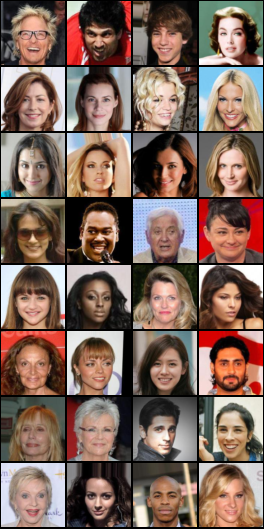
\includegraphics[width=\textwidth]{nifr/Images/celeba/vae_x_original.png}}%
      \label{fig:cvae_celeba_original_x}
  }
  \hfill
  \subfloat[$x_u$ null-samples generated by the \ac{cVAE} model.]{%
      \scalebox{0.3}{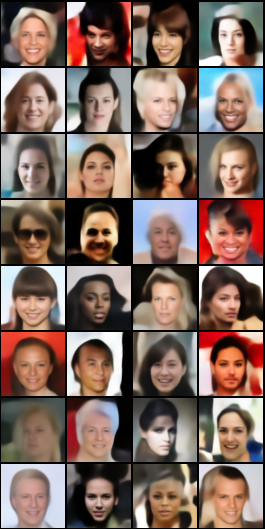
\includegraphics[width=\textwidth]{nifr/Images/celeba/vae_recon_y.png}}%
      \label{fig:cvae_celeba_recon_y}
  }
  \hfill
  \subfloat[$x_b$ null-samples generated by the \ac{cVAE} model.]{%
      \scalebox{0.3}{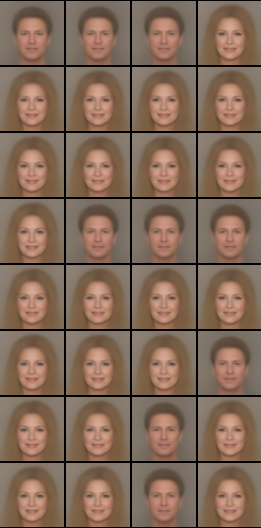
\includegraphics[width=\textwidth]{nifr/Images/celeba/vae_recon_s.png}}%
      \label{fig:cvae_celeba_recon_s}
  }
  \caption{
      CelebA null-samples learned by our \ac{cVAE} model, with gender as the sensitive attribute.
    %
    (a) The original, untransformed samples from the CelebA dataset
    %
    (b) Reconstructions using only information unrelated to $s$.
    %
    (c) Reconstruction using only information related to $\neg s$.
    %
    The model learns to disentangle gender from the non-gender related information. 
    %
    Compared with the \ac{cFlow} model, there is a severe degradation in reconstruction quality due to
    the model trying to simultaneously satisfy conflicting objectives.
    % Attributes such as \emph{make-up} and \emph{hair length} are also often modified in the
    % process due to inherent correlations between them and the sensitive attribute, which the
    % intepretability of our representations allows us to easily identify.
  }\label{fig:celeba_vae}
\end{figure*}

\begin{figure*}[tb]
  \centering
  \subfloat[Original images.]{%
      \scalebox{0.3}{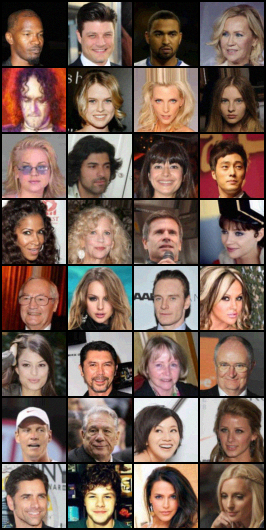
\includegraphics[width=\textwidth]{nifr/Images/celeba/cflow_original_x_suppmat.png}}%
      \label{fig:cflow_celeba_original_x_suppmat}
  }
  \hfill
  \subfloat[$x_u$ null-samples generated by the \ac{cFlow} model.]{%
      \scalebox{0.3}{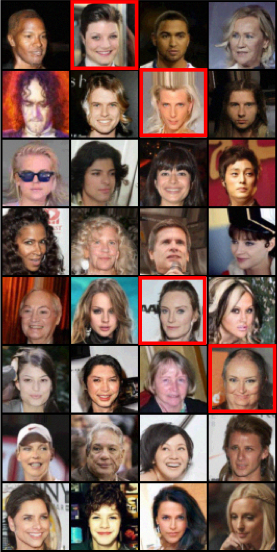
\includegraphics[width=\textwidth]{nifr/Images/celeba/cflow_xd_suppmat.png}}%
      \label{fig:cflow_celeba_recon_y_suppmt}
  }
  \hfill
  \subfloat[$\mathbf{x}_b$ null-samples generated by the \ac{cFlow} model.]{%
      \scalebox{0.3}{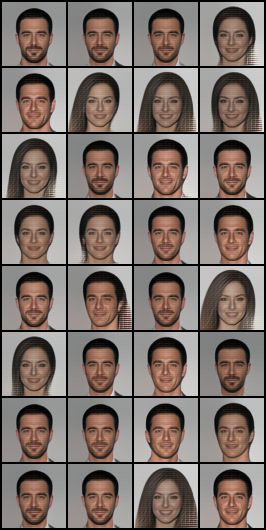
\includegraphics[width=\textwidth]{nifr/Images/celeba/cflow_xb_suppmat.png}}%
      \label{fig:cflow_celeba_recon_s_suppmat}
  }
  \caption{
      CelebA null-samples learned by our \ac{cFlow} model, with gender as the sensitive attribute.
    %
    (a) The original, untransformed samples from the CelebA dataset
    %
    (b) Reconstructions using only information unrelated to $s$.
    %
    (c) Reconstruction using only information related to $\neg s$.
    %
    The model learns to disentangle gender from the non-gender related information. 
    %
    Attributes such as \emph{make-up} and \emph{hair length} are also often modified in the process
    (prime examples framed with red) due to inherent correlations between them and the sensitive
    attribute, which the interpretability of our representations allows us to easily identify.
  }\label{fig:celeba_cflow_suppmat}
\end{figure*}

\subsection{Qualitative Results for CelebA}\label{sec:qual-results-celeba}
%
\noindent Learning a representation alongside its inverse mapping, be it approximate or exact,
enables us to probe the behaviour of the model that produced it, and any biases it may have
implicitly captured due to entanglement between the sensitive attribute and other attributes
present in the data. 
%
We highlight a few examples of such biases manifesting in the \ac{cFlow} model's CelebA null-samples in
Fig.~\ref{fig:celeba_cflow_suppmat}. 
%
In these cases, make-up and hair style have been inadvertently modified during the null-sampling
due to the tight correlation between these two attributes and the sensitive attribute, gender, to
which we had aimed to make our representations invariant. 
%
Additionally, in all highlighted images, the skin tone has changed: from male to gender-neutral,
the skin becomes lighter and from female to gender-neutral, the skin becomes darker; in the change
from male to gender-neutral, glasses are also often removed.
%
As the model cannot know that the label is meant to only refer to gender, and not to these other
(correlated) attributes, the links cannot be disentangled by the model.
%
However, the advantage of our method is that we can at least identify such biases due to the
interpretability that comes with the representations being in the data domain.

\begin{figure*}[htb]
  \centering
  \subfloat[Performance on cMNIST test data after pre-training on the mixed NIST dataset.]{
      \scalebox{0.6}{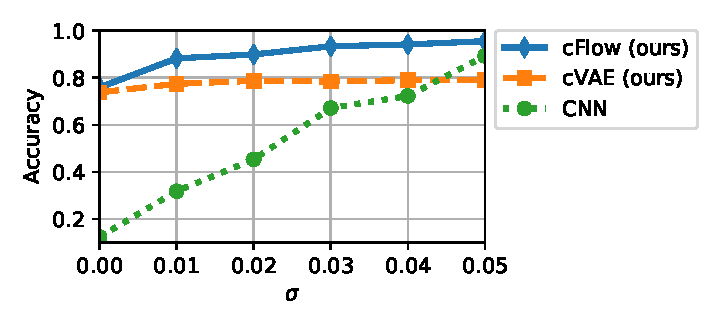
\includegraphics[width=\textwidth]{nifr/Figures/nosinn_cmnist_transfer.pdf}} \label{fig:cmnist-transfer}
  }
  %---
  \vspace{10pt}
 
  \subfloat[Test data input to the \ac{cFlow} model.]{%
      \scalebox{0.3}{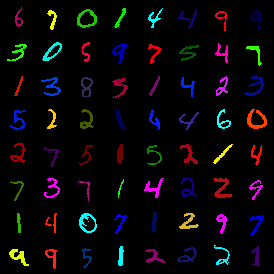
\includegraphics[width=\textwidth]{nifr/Images/cmnist/cflow_tl_original.png}}%
      \label{fig:cflow_tl_original}
  }
  ~~~
%   \hfill
  \subfloat[$x_u$ null-samples generated by the \ac{cFlow} model.]{%
      \scalebox{0.3}{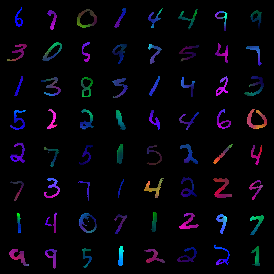
\includegraphics[width=\textwidth]{nifr/Images/cmnist/cflow_tl_xd.png}}%
      \label{fig:cflow_tl_xd}
  }
  
  \subfloat[Test data input to the \ac{cVAE} model.]{%
      \scalebox{0.3}{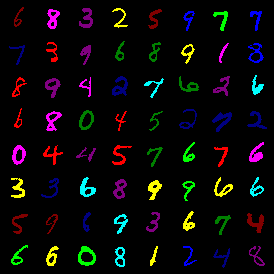
\includegraphics[width=\textwidth]{nifr/Images/cmnist/cvae_tl_original.png}}%
      \label{fig:cvae_tl_original}
  }
  ~~~
%   \hfill
  \subfloat[$x_u$ null-samples generated by the \ac{cVAE} model.]{%
      \scalebox{0.3}{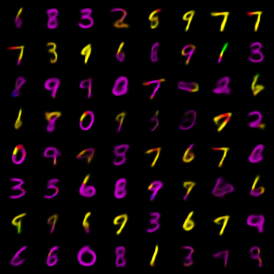
\includegraphics[width=\textwidth]{nifr/Images/cmnist/cvae_tl_xd.png}}%
      \label{fig:cvae_tl_xd}
  }
  \caption{
    Results for the transfer learning experiments in which the representative set consists of
    colourised samples from EMNIST, KMNIST, and FashionMNIST, while the downstream dataset remains
    as cMNIST. 
    %
    (a) Quantitative results for different $\sigma$-values. 
    %
    (b-c) Qualitative results for the \ac{cFlow} model. 
    %
    (d-e) Qualitative results for the \ac{cVAE} model. 
    %
    The qualitative results provide comparisons of the images before (left) and after (right)
    null-sampling. 
    %
    Note that for some of the \ac{cVAE} samples, the clarity of the digits has clearly changed due to
    null-sampling, serving as an explanation for the non-increasing downstream performance.
  }%
  \label{fig:cmnist-transfer-all}
  
\end{figure*}

\subsection{Transfer Learning}\label{sec:transfer-learning}
%
\noindent For our method, we require a representative set which follows the same distribution as
that observed during deployment. 
%
Such a representative set might not always be available. 
%
In such a scenario, we can resort to using a set that is merely \emph{similar} to that in the
deployment setting and leverage transfer learning.

%We argue that the inherent properties of INNs make them especially suitable for transfer learning.
One of the advantages of using an invertible architecture over conventional, \emph{surjective} ones
that we stressed in the main text is its \emph{losslessness}. 
%
Since the transformations are necessarily bijective, the information contained in the input can
never be destroyed, only redistributed. 
%
This makes such models particularly well-suited, in our minds, for transferring
learned invariances: even if the input is unfamiliar, no information should be lost when trying to
transform it. 
%
This works as long as only the information about $s$ ends up in the $z_b$ partition.
%
If $s$ takes a form similar to that which we pre-trained on, and can thus be correctly partitioned
in the latent space, by complement we have the information about $\neg s$ stored in the $z_u$
partition, without presupposing similarity to the $\neg s$ observed during pre-training.
%
\paragraph{Transferring from mixed-NIST to MNIST.}
%
We test our hypothesis by comparing the performance of the \ac{cFlow} and \ac{cVAE} models pre-trained on a
mixture of datasets belonging to the NIST family, colourised in the same way as cMNIST, while the
downstream train and test sets remain the same as in the original cMNIST experiments. 
%
Specifically, we create this representative set by sampling 24,000 images (to match the cardinality
of the original representative set) from EMNIST (letters only; \citealp{cohen2017emnist}),
Fashion\-MNIST~\citep{xiao2017fashion} and KMNIST~\citep{clanuwat2018deep}, in equal proportion. 
%
We use the same architectures for the \ac{cVAE} and \ac{cFlow} models as we did in the non-transfer learning
setting. 
%
In terms of hyperparameters, the only change made was to the KL-divergence's pre-factor, finding it
necessary to increase it to $1$ to guarantee stability.

The results for the range of $\sigma$ values are shown in Fig.~\ref{fig:cmnist-transfer}.
%
Unsurprisingly, the performance of both models suffers when the representative and test sets do not
completely correspond. 
%
However, the \ac{cFlow} model consistently outperforms the \ac{cVAE} model, with the gap increasing as the
bias decreases. 
%
Although some colour information is retained in the \ac{cFlow} null-samples, symptomatic of an imperfect
transfer, semantic information is almost entirely retained as well. 
%
Conversely, the \ac{cVAE} is very much flawed in this respect; as can be seen in the bottom row of
Fig.~\ref{fig:cmnist-transfer}, for some samples, semantic information is degraded to the point of
the digit's identity being altered. 
%
As a result of this semantic degradation, the performance of the downstream classifier is curtailed
by the noisiness of the digit's identity and is relatively unchanging across $\sigma$-values, in
contrast to the monotonic improvement of that achieved on the \ac{cFlow} null-samples.

% \begin{figure}
%   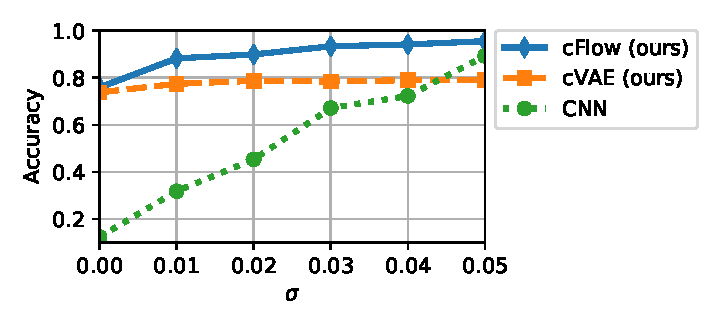
\includegraphics[width=0.6\textwidth]{nifr/Figures/nosinn_cmnist_transfer.pdf}
%   \caption{
%      Results for transfer learning experiments on cMNIST.
%   }%
%   \label{fig:cmnist-transfer}
% \end{figure}

% \clearpage

% \bibliographystyle{splncs04}
% \bibliography{references.bib}

% \end{appendix}

% \end{document}

\clearpage
\section{Authorial contributions}
%
{\renewcommand\labelitemi{}
%
\begin{itemize}
    %
    \item 
        %
        \textbf{T. Kehrenberg} conceived of the idea of using an INN combined with a
        representative set to learn an invariant representation in the face of spurious
        correlations, ran many of the experiments -- especially so in the initial stages -- and
        wrote much of the original text and code.
        %
    \item 
        %
        \textbf{I} wrote a significant part of the code (being responsible for several refactorings
        as part of the debugging process), the much of the text, helped crystallise the initial
        idea, ran many of the experiments, aided in experimental analysis, and developed much of
        the technical tricks needed to train the INN stably within the adversarial framework
        (grappling with the issues later elucidated by \citet{behrmann2021understanding}).
        %
    \item 
        %
        \textbf{O. Thomas} aided in writing the code, in running the experiments, partook in
        discussion and analysis of results, helped writing and formatting the paper, and served as
        an unwavering source of optimism.
        %
    \item
        %
        \textbf{N. Quadrianto} supervised the project, providing feedback on current progress and
        iterations of the paper and advising which directions to pursue.
        %
    %
\end{itemize}
%
}


  \printbibliography
\end{refsection}
%
\begin{refsection}[supmatch]
  % -------------------------------------------------------------------------------
\chapter{Addressing Missing Sources with Adversarial Support-Matching}\label{ch:supmatch}
% -------------------------------------------------------------------------------
\textsc{Authors}:\\
%
Thomas Kehrenberg$^1$, 
  %
Myles Bartlett$^1$,
  %
Viktoriia Sharmanska$^{1, 2}$ \& 
  %
Novi Quadrianto$^{1,3,4}$ \\
%
\textsc{Affiliations}:\\
  %
$^1$Predictive Analytics Lab (PAL), University of Sussex, Brighton, United Kingdom \\
  %
$^2$Imperial College London \\ 
  %
$^3$BCAM Severo Ochoa Strategic Lab on Trustworthy Machine Learning \\
  %
$^4$Monash University, Indonesia \\
%

\section*{Abstract}
\noindent
%
When trained on diverse labelled data, machine learning models have proven themselves to be a
powerful tool in all facets of society.
%
However, due to budget limitations, deliberate or non-deliberate censorship, and other problems
during data collection and curation, the labelled training set might exhibit a systematic dearth of
data for certain groups. This problem is particularly pertinent in medical imaging where the number
of positive samples typically outweigh the number of negative samples by an orders of magnitude and
certain demographics may be excluded on safety grounds (e.g. pregnant women) or due to
socioeconomic biases.
%
We investigate a scenario in which the absence of certain data is linked to the second level of a
two-level hierarchy in the data.
%
Inspired by the idea of protected groups from algorithmic fairness, we refer to the partitions
carved by this second level as ``subgroups''; we refer to combinations of subgroups and classes, or
leaf nodes in aforementioned hierarchy, as \emph{sources}.
%
To characterize the problem, we introduce the concept of classes with \emph{incomplete subgroup
support}. The representational bias in the training set can give rise to spurious correlations
between the classes and the subgroups which cause standard classification models to generalize
poorly to unseen sources.
%
To overcome this bias, we make use of an additional, diverse but unlabelled dataset, called the
\emph{deployment set}, to learn a representation that is invariant to subgroup. This is done by
adversarially matching the support of the training and deployment sets in representation space
using a set discriminator operating on sets, or \emph{bags}, of samples.
% that uses a set-based loss function inspired by multiple instance learning.
%
In order to learn the desired invariance, it is paramount that the bags are balanced by class; this
is easily achieved for the training set, but requires using semi-supervised clustering for the
deployment set.
%
We demonstrate the effectiveness of our method on several datasets and
realisations of the problem.

\label{sec:sm-abstract}

\section{Introduction}
\label{sec:sm-intro}
\begin{figure}[tb]
    \centering
    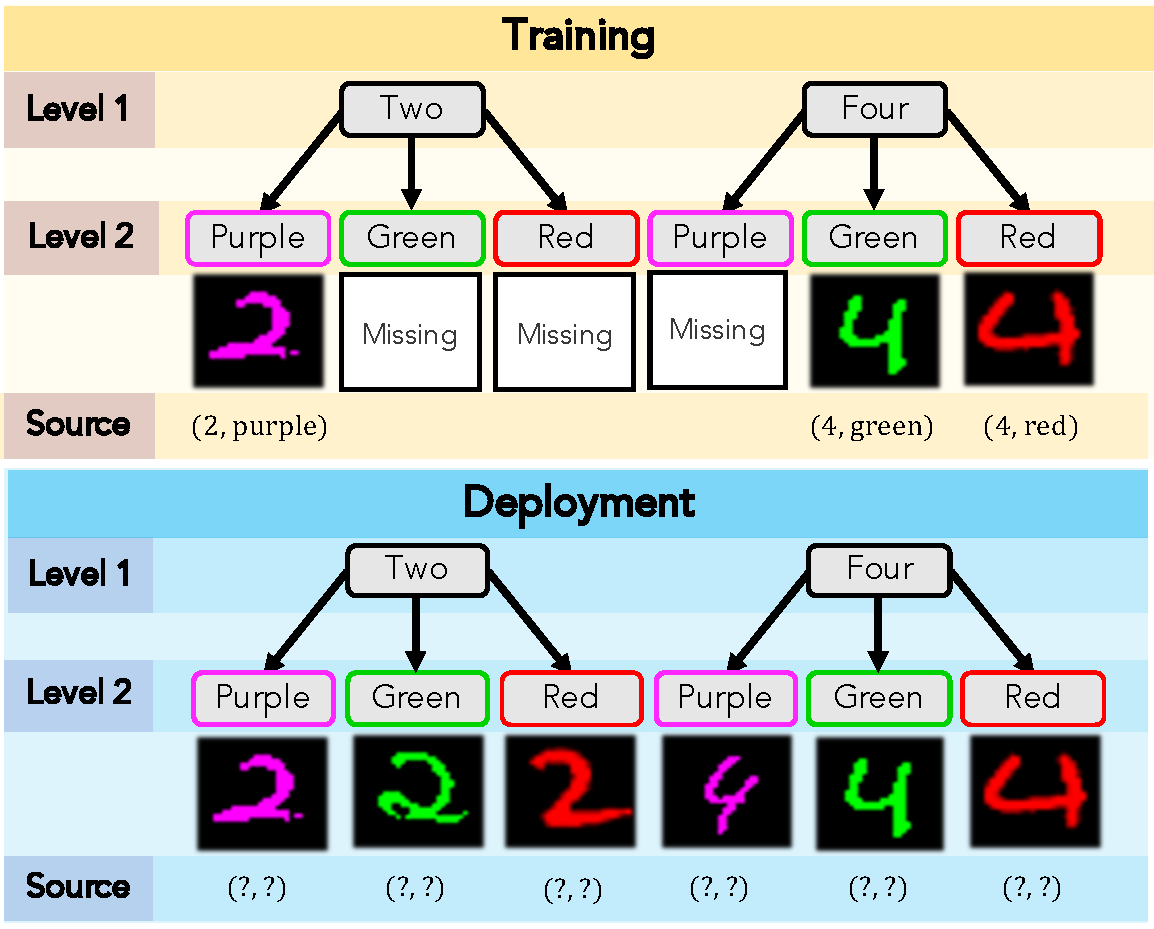
\includegraphics[width=0.7\columnwidth]{supmatch/figures/illustrations/problem_setup.pdf}
    \caption{%
      Illustration of our general problem setup. 
      %
      We assume the data follows a two-level hierarchy in which the first level corresponds to the class-level information (digit) and the second level corresponds to subgroup-level information (color).
      %
      While all digits appear in the training set (Top), not all digit-color combinations (sources) do; these gaps in conditional support give rise to a spurious correlation between digit and color, where the former is completely determined by the latter in the training set (giving the mappings $\textrm{{\color{purple}purple}} \rightarrow \texttt{2}$ and $\textrm{{\color{green}green}} \lor \textrm{{\color{red}red}} \rightarrow \texttt{4}$ as degenerate solutions to the classification problem), yet this same correlation does not hold for the deployment set (Bottom) which contains samples from the missing combinations.
      %
      To disentangle the (spurious) subgroup- and class-related information, we make use of an additional dataset that is representative of the data the model is expected to encounter at deployment time, in terms of the sources present.
    }%
    \label{fig:problem-setup}
\end{figure}


Machine learning has burgeoned in the last decade, showing the ability to solve a wide variety of
tasks with unprecedented accuracy and efficiency.
%
These tasks range from image classification \citep{krizhevsky2012imagenet} and object detection
\citep{ren2015faster}, to recommender systems \citep{ying2018graph} and the modelling of complex
physical systems such as precipitation \citep{ravuri2021skillful} and protein folding
\citep{jumper2021highly}.
%
In the shadow of this success, however, one finds less cause for optimism in frequent failure in
equitability and generalisation-capability, failure which can have serious repercussions in
high-stakes applications such as self-driving cars \citep{sun2019unsupervised}, judicial
decision-making \citep{mayson2018bias}, and medical diagnoses \citep{albadawy2018deep}.
%
ML's data-driven nature is a double-edged sword: while it opens up the ability to learn patterns
that are infeasibly complex for a practitioner to encode by hand, the quality of the solutions
learned by these models depends primarily on the quality of the data with which they were trained.
%
If the practitioner does not properly account for this, models ingesting data ridden with biases
will assimilate, and sometimes even amplify, those biases.
%
The problem boils down to not having sufficiently diverse annotated data, however collecting more
labelled data is not always feasible due to temporal, monetary, legal, regulatory, or physical
constraints.

%
While data can be intrinsically biased (such as in the case of bail records),
\emph{representational bias} is more often to blame, where socioeconomic or regulatory factors
resulting in certain demographics being under- (or even un-) represented. 
%
Clinical datasets are particularly problematic for ML due to the frequency of the different
outcomes being naturally highly imbalanced, with the number of negative cases (\texttt{healthy})
typically greatly outweighing the number of positive cases (\texttt{diseased}); even if a subgroup
is well-represented overall, that may well not be the case when conditioned on the outcome.
%
Equally, it is entirely possible that certain subgroups may be completely absent. 
%
For example, pregnant women are often excluded from clinical trials due to safety concerns, and if
they do participate it is often at too low a rate to be meaningful \citep{afrose2021overcoming}.

Like many prior works
\citep{SohDunAngGuetal20,kim2019learning,creager2021environment,SagRagKohLia20}, we consider
settings where there is a two-level hierarchy, with the second level partitioning the data into
\emph{subgroups} that are causally independent of the class (constituting the first level) which is
being predicted. 
%
This second level of the data is assumed to be predictable by the classifiers in the considered
hypothesis class. 
%
In both \citet{SohDunAngGuetal20} and \citet{creager2019flexibly} the entailed subgroups are
unobserved and need to be inferred in a semi-supervised fashion. We consider a similar problem but
one where the second level is partially observed.
%
Specifically, we focus on problems where some outcomes are available for some subgroups and not for
others. 
%
This particular form of the problem has -- so far as we are aware -- been hitherto overlooked
despite pertaining to a number of real-world problems.

%
If the labelled training set is sufficiently balanced in terms of classes and subgroups, a standard
ERM (empirical risk minimisation) classifier can achieve good performance.
%
However, we consider the added difficulty that, in the labelled training set, some outcomes
(classes) are not observed for all subgroups, meaning some of the classes do not overlap with all
the subgroups.
%
In other words, in the training set, some of the classes have \emph{incomplete support} with
respect to the subgroup partition, while in the deployment setting we expect all possible
combinations of subgroup and class to appear.
%
We illustrate our problem setup in Fig.~\ref{fig:problem-setup}, using Coloured MNIST digits as
examples; here, the first level of the hierarchy captures digit class, the second level, colour. 
%
While the (unlabelled) deployment set contains all digit-colour combinations (or \emph{sources}),
half of these combinations are missing from the (labelled) training set. 
%
A classifier trained using only this labelled data would wrongly learn to classify \texttt{2}s based
on their being {\color{purple}purple} and \texttt{4}s, based on their being {\color{green}green} or
{\color{red}red} (instead of based on shape) and when deployed would perform no better than random
due to the new sources being coloured contrary to their class (relative to the training set).

We address this problem by learning representations that are invariant to subgroups and that thus
enable the model to ignore the subgroup partition and to predict only the class labels.
%
In order to train an encoder capable of producing these representations, the information contained
in the labelled training set alone is not sufficient to break the \emph{spurious correlations}.
%
To learn the ``correct'' representations, we make use of an additional unlabelled dataset with
support equivalent to that of the deployment set (which includes the possibility of it being the
actual deployment set).
%
We do not consider this a significant drawback as such data is almost always far cheaper and less
labour-intensive to procure than \emph{labelled} data (which may require expert knowledge).
%

This additional dataset serves as the inductive bias needed by the encoder to disentangle class-
and subgroup-related factors.
%such that a downstream predictor can be trained using the available labels without risk of
%internalizing the spurious correlations present in the original data.
%
The encoder is trained adversarially to produce representations whose source (\texttt{training} or
\texttt{deployment}) is indeterminable to a set-classifier.
%
To ensure subgroup- (not class-) invariance is learned, the batches fed to the discriminator need
to be approximately balanced, such that they reflect the support, and not the shape, of the
distributions. 
%
We propose a practical way of achieving this based on semi-supervised clustering.
%

We empirically show that our proposed method can effectively disentangle subgroup and semantic
factors on a range of classification datasets and is robust to noise in the bag-balancing, to the
degree of outperforming the baseline methods even when no balancing of bags from the deployment set
is performed.
%
Furthermore, we prove that the entailed objective is theoretically guaranteed to yield
representations that are invariant to subgroups and that we can bound the error incurred due to
imperfect clustering.



\section{Problem setup}
\label{sec:sm-problem-setup}
% -------------------------------------------------------------------------------
In this section, we illustrate and formalise the problem of classes with incomplete
subgroup-support. 
%
We start by defining requisite notation for conveying our setup and in
\S\ref{ssec:problem_formalism} expand on this notation to construct a more general and compact
description of said problem. 
%
Let \( x \in \gX \subset \R^d \), \( y \in \gY \) and \( s \in \gS \) denote the observed input
features, class labels and subgroup labels, respectively, with \( \gY \) and \( \gS \) being
non-empty, finite sets (i.e.\ \( \gY, \gS \in \{ A | A \in \gP(V), A \neq \varnothing, |A| <
\aleph_0 \} \)), and with upper-case letters denoting observed variables' random-variable
counterparts here (\(X\), \(Y\), and \(S\)) and throughout.
% the set-builder notation S = {A | A ∈ P(X), A ≠ ∅, |A| < ∞} defines the set of all non-empty,
% finite sets that are subsets of the set X.
%
We refer to the values, \( g \in \gG \) as \emph{sources}, representing unique pairs of \( s \) and
\( y \), such that \(  \gG \subseteq \gS \times \gY \). 
%
As in a standard supervised learning task, we have access to a labelled training set \( \gD^{tr}
\triangleq \{ (x_n, s_n, y_n) \}_{n=1}^{N^{tr}} \subset (\gX \times \gS \times \gY) \), that is used to
train a classifier \( \Gamma:\gX \rightarrow \gY \) that is then deployed on test set \( \gD^{te}
\triangleq \{ (x_n, s_n, y_n) \}_{n=1}^{N^{te}} \subset (\gX \times \gS \times \gY) \). 
%
We use superscript, to denote association of a domain with a correspondingly superscripted dataset,
e.g.\ \( \gG^{tr} \) and \( \gG^{te} \) respectively denote the sources in the training and test
sets.
%
Lastly, for some functions, we abuse notation and allow the random and observed variables to be
interchanged as inputs; we presuppose such functions (and their domain) are Borel measurable and
thus preserve the type of variable, i.e.\ a function of a random variable is also a random
variable.
%
For example, given function \(f: \gX \to \R \), we may write both \( f(x) \) and \( f(X) \),
meaning by the latter \( f \circ X(\omega) \) for some event \( \omega \in \Omega \).
%
% -------------------------------------------------------------------------------
\subsection{Spurious correlations from missing sources}\label{ssec:walkthrough}
% -------------------------------------------------------------------------------
The spurious correlation (\ac{SC}; \citealp{arjovsky2019invariant}), or shortcut-learning
\citep{valle2018deep, geirhos2020shortcut}, problem is characterised by the presence of some
secondary attribute \(s\) (such as background \citep{beery2018recognition}, texture
\citep{geirhos2018imagenet}, or gender \citep{sagawa2019distributionally, seyyed2020chexclusion}
that confounds the prediction task.
%
We refer to this attribute as the ``subgroup'', in line with algorithmic fairness (\ac{AF};
\citet{barocas-hardt-narayanan}) that is strongly correlated with the target attribute, \(y\), in
the training set, but spuriously so in the sense that the correlation the mapping \( \gS \to \gY \)
is acausal and thus cannot be expected to hold at deployment time. 
%
This correlation is pernicious when \(S\) is of lower complexity (which can be formalised in the
Kolmogorov sense; \citet{scimeca2021shortcut}) than the causal cues contained in \(X\), and thereby
becomes the preferred cue by virtue of simplicity bias \citep{valle2018deep}. 
%
Such problems have garnered considerable attention in recent years \citep{liu2021just,
pezeshki2021gradient, SohDunAngGuetal20, krueger2021out} due to their pervasive, and potentially
catastrophic \citep{codevilla2019exploring, de2019causal, castro2020causality}, nature.
%
In this paper, we introduce, and propose a semi-supervised solution for, a hierarchical and
class-asymmetric variant of the \ac{SC} problem that we term the \emph{\acf{MS}} problem .

To illustrate the general \ac{SC} problem and the \ac{MS} problem as a particular instantiation of
it, we define the conditional-probability matrix, \( \mathbf{P}^{tr} \in [0, 1]^{|\gS| \times
|\gY|} \), where each element \( \mathbf{P}^{tr}_{ij} \) encodes the conditional probability \(
P^{tr}(Y=j|S=i) \) in the training set, \( \gD^{tr} \). 
%
When \( \mathbf{P}^{tr} \) is both binary and doubly stochastic (that is, has all rows and columns
summing to 1) we have that \(y\) is completely determined by \(s\) in \( \gD^{tr} \) -- this is an
extreme form of the \ac{SC} problem which is statistically intractable without access to additional
sources of data \citep{KehBarThoQua20} or multiple environments \citep{arjovsky2019invariant}. 
%
The \ac{MS} problem can be viewed as a relaxation of this \ac{SC} wherein the elements of \(
\mathbf{P}^{tr} \) respect the constraint that all columns contain at least one non-zero value,
i.e.\ we observe all class labels but not all possible pairs of class and subgroup labels -- we say
that we have \emph{missing sources}, \(\gM\ \triangleq \gG^{te} \setminus \gG^{tr}\). 
%
This setup still leads to spurious correlations but ones that are statistically tractable due to
asymmetry.
%
Practically speaking, considering only cases where sources are entirely missing is overly
restrictive, and as such we instead view the problem setup as extending to cases where sources may
not be altogether missing but have sample sizes too small to constitute meaningful supervision. 
%
To understand the non-triviality of this problem, and why aiming for invariance to \(s\) in the
training set alone -- as is characteristic of many representation-learning methods in \ac{AF}
\citep{edwards2015censoring, madras2018learning, quadrianto2019discovering}  and domain adaptation
(\ac{DA}; \citep{ganin2016domain, zhao2018adversarial, saito2018maximum, lee2019sliced}) -- will
assuredly fail, consider a binary classification problem with binary subgroups, where \(\gY = \{ 0,
1 \}\) and \( \gS = \{ 0, 1 \}\) and for which \( \mathbf{P}^{tr} \) takes the form
%
\begin{align}\label{ms_example}
  \mathbf{P}^{tr} = \bordermatrix{
  & Y=0 & Y=1 \cr
  S=0 & 0.5 & 0.5 \cr
  S=1 & 1.0 & 0.0}~.
\end{align}
%
This represents a special case of the \ac{MS} problem that we refer to as the \emph{Subgroup Bias}
(SB) problem, distinguished by the fact that we observe all subgroups. 
%
Here, we have samples from $S=0$ evenly distributed across both the negative and positive classes;
for $Y=1$, however, we only observe samples from the negative class. 
%
This setup might appear somewhat benign at first blush, given that all classes are present in the
training set, however, the fact that \(s\) serves as a proxy for \(y\) in the case of $S=1$
frustrates our goal of subgroup-invariant classification. 
%
The reason for this becomes obvious when decompose a classifier into a mixture of experts (MoE),
where \(s\) indicates which expert to choose for the given sample. 
%
Such a model naturally arises in practice due to the tendency of deep neural networks to strongly
favour shortcut solutions \citep{geirhos2020shortcut}.
%
We note that for this, and throughout the paper, we assume that \(s\) is inferable, to some extent,
from $x$, that is \( \gI(X; S) > 0 \), with \( \gI(\cdot; \cdot) \) denoting the mutual information
between two variables -- this is almost always the case in practice but we make the dependence
explicit here by denoting by \( X_Y \) the causally-relevant component of \( X \)), that is
independent of \(S\), and by including \( s \in \{0, 1\} \) explicitly in the set of inputs.
%
With this noted, we may then define the MoE classifier, \(c_{MoE}\), that `solves' the training set
with labels distributed according to \( \mathbf{P}^{tr} \) as
%
\begin{align}
  c_{MoE}(X_Y, S) = \begin{cases}
c_{S=0}(X_Y) &S=0 \\
0 &S=1 \\
\end{cases},
\end{align}
%
using \(c_{S=0}(\cdot)\) to denote the expert that learns to classify only the subset of the data
for which $S=0$.
%
Such a classifier is clearly undesirable, as should it ever encounter a sample belonging to
subgroup $1$ with a positive label, the classifier will automatically declare it negative without
needing to attend to $X_Y$ -- it is invariant to $X_Y$ while being variant to \(S\), which is the
opposite of what we desire. 
%
This is often done by learning an encoder $f: \gX \to \gZ$ that maps an input $x$ into a
representation, \( z \in \gZ \subset \R^l \), which has the desired property of \(S\)-invariance,
\( Z \perp S \), while also maximising $\gI(Z; Y)$ so that the representation is useful for
classification. 
%
A popular way of imparting this invariance is with adversarial methods \citep{ganin2016domain,
zhao2018adversarial, madras2018learning} where  $f$ is trained to the equilibrium point, $f^\ast$,
of the (non-convex) minimax equation 
%
\begin{align}\label{eq:moo}
\underset{f \in \gF}{\text{min}}\; \underset{a \in \gA}{\text{max}}\,
\E_{(x, s, y) \sim \gD^{tr}}
\big[ 
  \textcolor{red}{ \overbrace{ a(f(x))_s }^{ \text{invariance}} }
  - \textcolor{blue}{ \underbrace{ \lambda \gI(f(x); y) }_{ \text{classification} } }
\big],
\end{align}
%
where \( a: \gZ \to \bigtriangleup^{|\gS|} \) is a parametric adversary with codomain the standard
simplex over \( \gS \), and \(\lambda \in \R^+\) is a positive scalar controlling the trade-off
between the two constituent objectives. 
%
Under ideal conditions, when all possible pairs of \(s\) and \(y\) are observed, \(f^\ast\)
corresponds to the point at which \(a\) is maximally entropic and occurs when \(Z\) is invariant to
\(S\), and only \(S\), while mutual information \wrt{} \(Y\) is jointly maximised -- from an
optimisation standpoint, the gradients of first and second objectives are non-conflicting (i.e.\
have non-negative inner products; \citealp{yu2020gradient}) and there is no trade-off. 
%
However, in cases where we have missing sources, the waters are muddied: satisfying the first part
of the objective connotes invariance not only to \(S\), but also to \(Y\), since \(S\) can be
predicted from \(Y\) with above-random accuracy due to the skewed statistics of the dataset. 
%
This is patently problematic as \(Y\) is the very thing we wish to predict and achieving invariance
to \(S\) does little good if our classifier can no longer utilise features predictive of \(Y\). 

Since we cannot achieve optimality for the competing invariance and classification terms
simultaneously, we instead have a set of \ac{PO} solutions that collectively make up the Pareto
front -- learning the solutions corresponding to different trade-offs, or preference vectors, is
the domain of \acl{MOO} (\acs{MOO}; \citealp{deb2014multi}). 
%
Specifically, Eq.~\ref{eq:moo}, with \(\lambda\) controlling the preference direction,
characterises the most straightforward approach to MOO, called \emph{linear scalarisation}
\citep{boyd2004convex}. 
%
\Ac{MOO} has recently been explored in the context of \ac{UDA}, for controlling the descent
direction, in unsupervised domain adaptation (UDA) in light of the conflict arising between the
gradients of the alignment and classification terms \citep{liang2021pareto}, and in \acf{AF} for
controlling the inherent trade-off between predictive performance and fairness (typified by the
\emph{Accuracy-Fairness trade-off}; \citet{martinez2020minimax}).
%
While our missing-sources problem admits a \acs{MOO}-based approach, we are instead interested in
leveraging unlabelled data to sidestep the implied trade-off altogether.
% -------------------------------------------------------------------------------
\subsection{Formalising the problem}\label{ssec:problem_formalism}
% -------------------------------------------------------------------------------
In order to provide a general formulation of the \ac{MS} problem exemplified above, we begin by
defining additional notation for reasoning over label-conditioned subsets and their support. 
%
For a given dataset, \( \gD \), we denote by \( \gD_{S=s^\prime} \) its subset with subgroup label
\( s^\prime \in \gS \), by \( \gD_{Y=y^\prime} \) its subset with class label \( y^\prime \in \gY
\), and -- combining the two -- by \( \gD_{S=s^\prime,Y=y^\prime} \) its subset with subgroup label
\( s^\prime \) and class label \( y^\prime \).
%
According to this scheme, \( \gD_{S=\text{\color{purple}{purple}}, Y=\text{2}} \) should then be
read as ``the set of all samples in \( \gD \) with class label `2' and subgroup label
`\textcolor{purple}{purple}'''.
%
We apply similar syntax to the subgroups, writing \( \gS^{tr}_{Y=y^\prime} \) to mean the observed
subgroups within class \(y\) in the training set.
%
For instance, \(\gS^{tr}_{Y=1}=\{0\}\) prescribes that for class \(1\), only subgroup \(0\) is
present in the training set.

We assume a problem of a hierarchical nature.
%, as illustrated in Fig.~\ref{fig:problem-setup}. 
%
While the full set of class labels is observed in both the training and test sets, we do not
observe all pairs of \(s\) and \(y\) in the former, i.e.\ \( \gG^{tr} \subset \gG^{te} \) or \(\gM
\neq \varnothing \). 
%
Equivalently, we say that for some class, \(y^\dagger\), we have \( \gS^{tr}_{Y=y^\dagger} \subset
\gS \), subject to the constraint that \(  \gS^{tr} = \gS^{te} \).
%
With this, we can succinctly notate the SB problem realised by Eq.~\ref{ms_example}, in which class
\(Y=1\) has no overlap with subgroup \(S=1\), as \(\gS^{tr}_{Y=1}=\{0\}\) (while
\(\gS^{tr}_{Y=0}=\{ 0, 1 \}\)), corresponding to \( \gM = \{(1, 1)\} \), and distinguish SB
problems generally by the inclusion of the additional constraint \( \gS^{tr} = \gS^{te} \).
%
To illustrate a more complex case, the SB problem depicted in Fig.~\ref{fig:problem-setup}, in
which for we observe exclusively purple `2's and green and red `4's, can be notated with the pair
\( \gS^{tr}_{Y=2}=\{\text{\textcolor{purple}{purple}\}} \), \( \gS^{tr}_{Y=4}=\{
\text{\textcolor{green}{green}}, \text{\textcolor{red}{red}} \} \).
% -------------------------------------------------------------------------------
\subsection{A way forward}
% -------------------------------------------------------------------------------
In this paper, we propose to alleviate the SB problem by mixing labelled data with
\emph{unlabelled} data that is usually much cheaper to obtain \citep{ChaSchZie06}, referring to
this set of \emph{unlabelled} data as the \emph{deployment set} 
%
\footnote{In our experiments, we report accuracy and bias metrics on another independent test set
instead of on the unlabelled data that is available at training time.} \( \gD^{dep}_\star =\{(x_n,
s_n^\star, y_n^\star)\}_{n=1}^{N^{dep}} \subset (\gX \times \gS \times \gY) \), using ``\(\star\)''
to denote that the labels are \emph{unobserved}, and in practice we only have access to \(
\gD^{dep} \triangleq \{(x_n)\}_{n=1}^{N^{dep}} \subseteq \gX \) and must estimate the corresponding
sources.
%
We assume that this deployment set is source-complete \wrt{} the test set, \( \gG^{dep} = \gG^{te}
\). Leveraging this deployment set, we seek to learn a classifier, \( \Gamma \), that can
generalise well to the missing sources appearing in the test set without seeing any labelled
representatives in the training set. 
%
In practice, we treat \( \Gamma \) as a composition, \( c \circ f \), of two subfunctions: an
encoder \( f: \gX \to \gZ \), which maps a given input \( x \) to a representation \( z \in \gZ
\subseteq \R^l \), and a classifier head \( c: \gZ \to \gY \) which completes the mapping to the
space of class labels, \( \gY \). 
%
Since the task of achieving independence between the predictions and subgroup labels can be reduced
to the task of learning the invariance \( Z \perp S \); we next discuss how one can learn an
encoder satisfying this condition in a theoretically-principled manner.
% -------------------------------------------------------------------------------
% % ********************************************************************************
\section{Some notes on notation}\label{sec:notation}
% ********************************************************************************
We describe here some of the general notation schemes used throughout this background chapter,
leave the concrete notation to be defined contextually, both to allow overloading (to allow for
reuse and restrictedness of the alphabet) and to minimise cognitive overhead for the reader.

%
First, we denote random variables using upper-case (non-calligraphic) letters and their associated
observed/deterministic/realised variables with the corresponding lower-case letters.
%
Following convention, we consistently denote by \(X\) and \(Y\) the input (covariate) and
target (response) variables, respectively; by \(S\) some auxiliary variable on which we want to
condition (for evaluation and/or optimisation), such as the domain (in domain
adaptation/generalisation) or sensitive attribute (in algorithmic fairness); by \(Z\) the latent
space, representations, encodings, or embeddings (all synonymously) of some model.
%
Second, calligraphic letters are used to denote (but not exclusively) the domain of a variable,
e.g. \(x \in \gX \).
%
Under this scheme, we would have for the random variable, \(X: \Omega \to \R^d \), realisations \(x
\in \gX \subset \R^d \) defined on a subset of the \(d\)-dimensional space of real numbers.
%
We then use \(P(\cdot)\) to denote probability distributions with conditioning indicated as
\(P(X=x)\) -- continuing the foregoing example -- and use \(\gD\) to denote \emph{datasets} that
correspond to the empirical distributions of variables; for instance \(\gD \triangleq
\{x_i\}_{i=1}^N \) denotes a dataset made up of \(N\) observations of \(X\).
%
We will often augment this notation with super- and subscripts to indicate a variety of concepts
including, inter alia, association with a particular subset of the data or concept, optimality,
observability, and approximation.
%
Some representative examples include \(\gD^{tr}\) and \(\gD^{te}\) to denote the training and test
sets, respectively, \(f^\ast\) to denote the optimal function \wrt{} some optimisation problem, and
\(\hat{y}\) to denote a prediction made by some estimator (of \(P(Y|X)\)).
%
% We will state the exact meaning in each case, whenever it is not obvious by association.

%
Finally, to simplify exposition, we abuse notation by allowing functions of the form \(f: X \to Y
\) to accept random and observed variables interchangeably; we assume that the derived function
classes are Borel Measurable and as such that a function of a random variable is also a random
variable. \(f\) to operate on random variables \(X\).
% %
Thus, pedantically speaking, \( f(X) \) should be read as shorthand for \( f \circ X(\omega) \),
for some event \( \omega \) drawn from sample space, \( \Omega \), while \( f(x) \) should be read
in the standard fashion, with deterministic inputs and outputs.



\section{Adversarial support-matching}
\label{sec:sm-adversarialsm}
\begin{figure*}[tb]
  \centering
  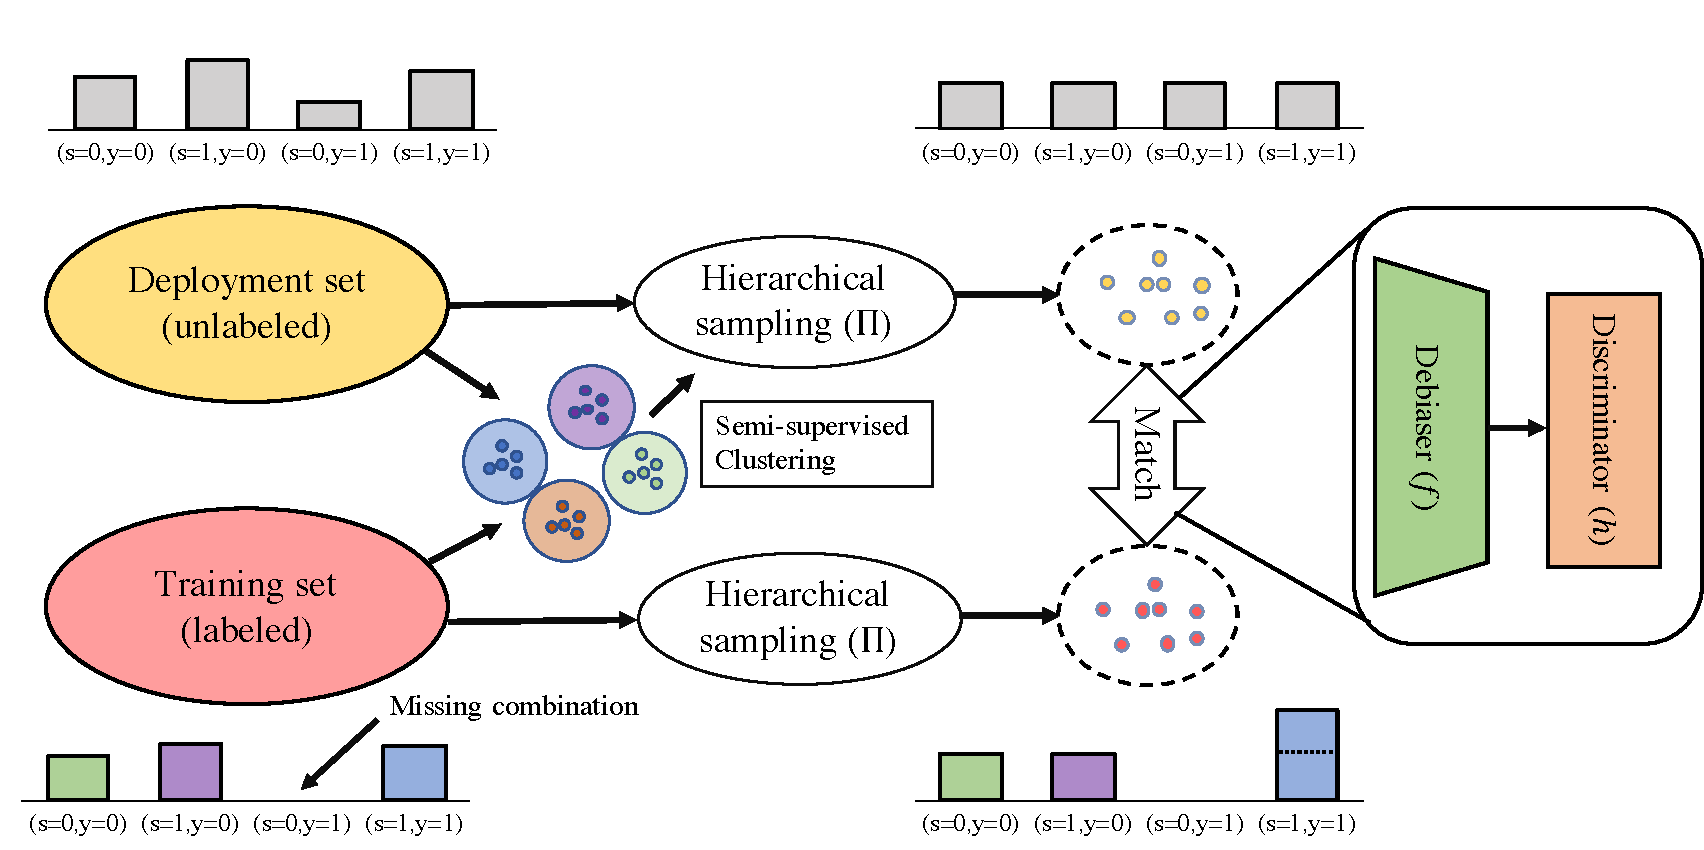
\includegraphics[width=1.0\textwidth]{supmatch/figures/illustrations/pipeline.pdf}
  \caption{%
    Visualisation of our support-matching pipeline.
    % A source is defined as certain combinations of the subgroup, s, and target class, y. Bags are
    % sampled from one of two datasets. The training set has labeled information about both $s$ and
    % $y$ but may be missing support over $S\times Y$. The deployment set on the other hand, is
    % assumed to have full support over $S \times Y$ but is unlabeled, meaning it cannot be used
    % for directly training a classifier. 
    Bags are sampled from the training and deployment sets using the hierarchical sampling
    procedure described in \S\ref{sec:sm-adversarialsm} and defined functionally in
    Eq.~\ref{eq:functional-sampling}. 
    %
    Since we cannot use ground-truth labels for hierarchical sampling of the deployment set, we use
    a semi-supervised clustering algorithm to produce balanced batches. In the event that certain
    combinations are missing, as shown here for $(s=0,y=1)$, the sampling on the training set
    substitutes the missing combinations with combinations that ensure equal representation of the
    target classes. 
    %
    The debiaser is adversarially trained to produce representations from which the source dataset
    cannot be reliably inferred by the discriminator. 
    %
    Assuming the bags are sufficiently balanced and $\gG^\mathit{tr}  \subsetneq \gG=\gS\times\gY$,
    the optimal debiaser is one that produces a representation $z$ that is invariant to $s$, which
    we prove in Appendix~\ref{implication-of-the-objective}.
    }%
  \label{fig:sm-pipeline}
\end{figure*}



We cast the problem of learning a subgroup-invariant representation as one of
\emph{support-matching} between a dataset that is \emph{labelled} but has \emph{incomplete} support
over sources, $G$, and one, conversely, that has \emph{complete} support over $G$, but is
\emph{unlabelled}. 
%
The idea is to produce a representation that is invariant to this difference in support, and thus
invariant to the subgroup. However, it is easy to learn the wrong invariance if one is not careful.
% Simply matching the distributions of the two datasets would wrongly result in the relative
% frequency of the sources being taken into account and the potential loss of task-relevant
% information.
To measure the discrepancy in support between the two distributions, we adopt an adversarial
approach, but one where the adversary is operating on small sets -- which we call \emph{bags} --
instead of individual samples. 
%
%
%
These bags need to be balanced with respect to ($s$, $y$), such that we can interpret them as
approximating $\gG$ as opposed to the joint probability distribution, $P(S, Y)$.
%
Details on how these bags are constructed can be found in in \S\ref{ssec:sm-realisation} and
\S\ref{sec:sm-implementation}.
% These sets correspond to the "perfect bags" introduced in the next section,
% \S\ref{ssec:perfect-bags}:


\subsection{Objective}\label{ssec:sm-objective}
%
We now present our overall support-matching objective. 
%
As alluded to before, the goal, in summary, is to learn an encoder, \(f\), which
preserves all information relating to $Y$, but is invariant to $S$. 
%if the training set is incomplete \wrt{} $s$.
Let \(P^{tr}(f(X)=z', S=s',Y=y')\) be the joint probability that a data point \(x\) drawn
from \(P^{tr}(X)\) -- the training set -- results in the encoding \(z'\) and is at the same
time labelled as subgroup \(s'\) and class \(y'\). 
%
We also define the following shorthand: $p_f(Z=z')=P^{tr}(f(X)=z')$, the distribution
resulting from sampling \(x\) from \(P^{tr}\) and then transforming \(x\) with \(f\).
%
Analogously for the deployment set: $q_f(Z=z')=P^{dep}(f(X)=z')$. 
%
For the conditioned distributions we write $p_f|_{S=s',Y=y'}$, following the convention established
in \S\ref{ssec:problem_formalism} but with the added `\(|\)' to clearly delimit the
conditioning.

The objective makes a distinction between those classes, \(y \in \gY\), for which there is overlap
with all subgroups \(s \in \gS\) in the training set and those classes for which there is not.
% An extreme version of this is when \emph{none} of the classes have overlap with a specific subgroup.
% In the \emph{missing subgroup} scenario, \emph{none} of the classes have overlap with all subgroups \(s\).
To formalise this, we define the following helper function $\Pi$ which maps \((s',y')\) to a set of
subgroup identifiers depending on whether the class \(y\) has full \(s\)-support:

\begin{align}\label{eq:Pi}
\Pi(s',y') = \begin{cases}
  \{s'\}&\text{if }\,\gS^{tr}_{ Y=y' }=\gS \\
  \gS^{tr}_{ Y=y' }&\text{otherwise.}
\end{cases}
\end{align}
%
$\Pi(s,y)$ ensures that the correct invariance is learned and is discussed in more detail further below.
Our objective is then
%
\begin{align}
  \gL_\text{match}(f)=\sum\limits_{s'\in\gS}\sum\limits_{y'\in\gY} d(p_f|_{s\in \Pi(s',y'),Y=y'},
  q_f|_{S=s',Y=y'})
\label{eq:objective}
\end{align}
%
where \(d(\cdot, \cdot)\) is a distance measure for probability distributions.
The optimal encoder $f^*$ is found by solving the following optimisation problem:
%
\begin{align}
  f^*=
  \argmin\limits_{f\in\gF} 
  \textcolor{red}{
  \gL_\text{match}(f)
  }
  - 
  \textcolor{blue}{
  \gI(f(X);X)
  }
\end{align}
%
where $\gI(\cdot; \cdot)$ again denotes the mutual information. As written, Eq.~\ref{eq:objective}
requires knowledge of \(s\) and \(y\) on the deployment set for conditioning. 
%
That is why, in practice, the distribution matching is not done separately for all combinations of
\(s'\in\gS\) and \(y'\in\gY\). 
%
Instead, we compare \emph{bags} that contain samples from all combinations in the right
proportions. For the deployment set, Eq.~\ref{eq:objective} implies that all
\(s\)-\(y\)-combinations have to be present at the same rate in the bags, but for the training set,
we need to implement \(\Pi(s',y')\) with hierarchical balancing.

As the implications of the given objective might not be immediately clear,
we provide the following proposition.
%
The proof can be found in Appendix~\ref{sec:sm-theoretical-analysis}.
%
\begin{theorem}
%
If \(f\) is such that
%
\begin{align}
p_f|_{s\in \Pi(s',y'),Y=y'} = q_f|_{S=s',Y=y'}\quad\forall s'\in\gS, y' \in\gY
\end{align}
%
and \(P^{tr}\) and \(P^{dep}\) are data
distributions that correspond to the real data distribution \(P\),
except that some \(s\)-\(y\)-combinations are less prevalent, or, in the
case of \(P^{tr}\), missing entirely, then, for every
\(y' \in \gY\), there is either full coverage of \(s\) for \(y'\)
in the training set (\( \gS^{tr}_{ Y=y' }=\gS \)), or the
following holds:
%
\begin{align}
P(S=s'|f(X)=z', Y=y')=\frac{1}{n_s}~.
\end{align}
%
In other words: for \(Y=y'\), \(f(x)\) is not predictive of \(s\).
\end{theorem}

\subsection{Implementation}\label{ssec:sm-realisation}
%
The implementation of above objective combines elements from unsupervised representation-learning and
adversarial learning.
% For simplicity, we follow an autoencoder paradigm for the former but any
% unsupervised/self-supervised representation learning objective could be used in place of the
% reconstruction objective.
In addition to the invariant representation $z$, our model also outputs $\tilde{s}$, in a similar
fashion to \citet{KehBarThoQua20} and \citet{creager2019flexibly}. 
%
This can be understood as a reconstruction of the subgroup information from the input $x$ and is
necessary to prevent $z$ from being forced to encode $s$ by the reconstruction loss.
%
We note that this need could potentially be obviated through use of self-supervised approaches,
but refrain from exploring this avenue in the interest of simplicity.

The model, \(\Gamma\), is composed of three core modules: 
1) two \emph{encoder} functions, $f$ (which we refer to
as the ``debiaser'') and $t$, which share weights and map $x$ to $z \in \gZ$ and
$\tilde{s} \in \tilde{\gS}$, respectively;
2) a \emph{decoder} function \(r: \gZ \times \tilde{\gS} \to \gX\) that learns to
invert $f$ and $t$; and
% 3) \emph{predictor} functions $\ell_y$ and $\ell_s$ that predict $y$ and $s$
% from $z$ and $\tilde{s}$ respectively, and
3) a \emph{discriminator} function \( h: (\mathfrak{Z} \subseteq \gP(Z)) \to ( 0, 1 ) \) that
predicts which dataset a bag of samples, \(\gB\ \in \mathfrak{Z}\), embedded in $\gZ$, was sampled
from, where we have used \( \gP(\cdot) \) to denote the powerset of its argument and thereby a
domain comprising sets of elements of \(\gZ\).
% The predictor $\ell_s: \tilde{\gS} \to \bigtriangleup^{|\gS|}$ (with $\bigtriangleup^{|\gS|}$
% denoting the $|\gS|$-dimensional standard simplex) is usually the identity function, and is
% primarily listed here for notational symmetry. Fig. \ref{fig:architecture} illustrates how $f$
% and $h$ interact during training -- the decoding step involving the other two components, $t$ and
% $g$, is omitted for compactness. This marks a significant departure from the typical GAN
% discriminator, which takes as input batches of data and yields a prediction for each sample
% independently of the other samples in the batch. %, where the training signal comes from the
% perfect dataset.
%
The encoder $f$ is then tasked with learning a representation $z$ such that it is indeterminable to
the adversary $h$ whether a given bag originated from the deployment set (`positive') or the
training set (`negative').
Formally, given bags
\( \gB^{tr} \), sampled according to \(\Pi\) from the training set, and balanced bags from the deployment
set, \( \gB^\mathit{dep} \), we first define, for notational convenience, the loss \wrt{} to the
encoder networks, $f$ and $t$ as
%
\begin{align}
&\gL_\text{enc}(f, t, r, h) = 
  \sum_{b^{dep} \in \gB^{dep}}
  \sum_{b^{tr} \in \gB^{tr}} 
\textcolor{blue}{
  \Bigg[\,
    \overbrace{
    \sum_{x \in b^{dep} \cup b^{tr}} 
      \lVert x - r(f(x), t(x))\rVert_p^p}^{\gL_{\text{recon}}}
    \Bigg]
    }
    \nonumber\\
   &\quad\quad\quad\quad\quad\quad
 %   +  
   \textcolor{red}{
     \underbrace{ \lambda_\text{match}  \Bigg[
       \log h \bigl( \{ \texttt{sg}[f(x)]\ | x \in b^\mathit{dep} \} \bigr) 
       - \log h \bigl( \{ f(x)\ | x \in b^\mathit{tr} \} \bigr) 
 \Bigg] }_{\gL_{\text{match}}}
},
   % \nonumber\\
   % &\quad+ \!\!\sum_{x\in b_\mathit{tr}}
   % \lambda_y L_{\text{sup}} (
   % y, \ell_y(f(x))) + \lambda_s L_{\text{sup}} (s, \ell_s(t(x)))
\label{eq:disentangling}
\end{align}
%
where \( \gL_{\text{recon}} \) denotes the reconstruction loss defined by the \(p\)-norm (\(p=1\)
and \(p=2\) yielding MAE and MSE, respectively), \( \gL_\text{match} \) denotes the adversarial loss,
\( \lambda_\text{match} \in \mathbb{R}^+_\ast \) is a pre-factor controlling the trade-off between
the loss terms, and \( \texttt{sg}[\cdot] \) denotes the ``stop-gradient`` operator that behaves as
the identity function but with zero partial derivatives.
%
The overall objective, encompassing $f$, $t$, and $h$ can then be formulated in terms of
\( \gL_\text{enc} \) as
%
\begin{align}
    \underset{f, t, r}{\textrm{min}}\; \underset{h}{\textrm{max}}\,\gL_\text{enc}(f, t, h)~.
    \label{eq:disentangling_total}
\end{align}
%
This equation is computed over batches of bags and the discriminator is trained to map a bag of
samples from the training set and the deployment set to a binary label: $1$ if the bag is adjudged to
have been sampled from the deployment set, $0$ if from the training set.
% Its goal is to effectively estimate the probability that a bag of samples has been sampled from
% one distribution or the other.
For the discriminator to be able to classify sets of samples, it needs to be permutation-invariant
along the bag dimension -- that is, its predictions should take into account dependencies between
samples in a bag while being invariant to the order in which they appear. 
% We experiment with two different types of attention mechanism for the bag-wise pooling layer of our
% discriminator, finding them both to work well.
\corr{
To aggregate information over samples within the bags, we employ a self-attention-based
\citep{vaswani2017attention} pooling layer, with aggregation achieved simply by setting the query
vector to be the mean of the (projected) representations over the bag dimension.
%
For more details, see Appendix~\ref{ssec:attention-mechanism}. 
%
Furthermore, in Appendix~\ref{ssec:no-mil}, we validate that having the discriminator operate over
sets (bags) of samples rather than independent samples (with the same balancing scheme) is
essential for achieving good and robust (\wrt{} balancing quality) empirical performance,
though we note that the two realisations yield minimax objects with theoretically-equivalent optima.
%
This observation on the difference in stability between the two realisations may have implications
for adversarial training more broadly, however we focus on the much narrower scope of the \ac{MS}
problem and leave it to future work to explore such implications.
}
% CORRECTION: there was a discussion of bags somewhere in this chapter ( i got a bit lost!) but as
% per the discussion in the viva discuss the influence of bags. potentially could be something to
% say as future work. Also could mention the use of the mean as the query in the attention
% mechanism could be good. Discuss with novi if this is novel enough to warrant taking further

% Our goal is to make $z$ invariant to the subgroup $s$. However, what the adversarial loss
% actually enforces is that $z$ generates bags with the same support over $S \times Y$ irrespective
% of the dataset they were drawn from. To ensure that the disentangling aligns with our objective,
Our goal is to disentangle $x$ into two subspaces: a subspace $z$, representing the class, and a
subspace $\tilde{s}$, representing the subgroup.
%
For the problem to be well-posed, it is crucial that the bags differ only
in terms of which sources are present and not in terms of other aspects.
% with respect to the class-subgroup combinations present and not with respect to the shape of the
% underlying distribution.
We thus sample the bags according to the following set of rules which operationalize $\Pi$. Please
refer to Fig.~\ref{fig:sm-pipeline} for a visualisation of the effect of these rules. 
%
\begin{enumerate}\label{ls:rules}
  %
  \item Bags of the deployment set are sampled so as to be approximately balanced with
    respect to $s$ and $y$ (all combinations of $s$ and $y$ should appear in equal number). 
    %
  \item For bags from the training set, all possible values of $y$ should appear with equal
    frequency. Without this constraint, there is the risk of $y$ being encoded in $\tilde{s}$
    instead of $s$. 
  \item Bags of the training set should furthermore exhibit equal representation of each subgroup
    within classes so long as rule 2 is not violated.
    For classes that do not have complete $s$-support, the missing combinations of $(s, y)$ need to
    be substituted with a sample from the same class -- i.e., if $s \notin \gS^{tr}(y)$ we instead
    sample randomly from a uniform distribution over $\gS^{tr}(y$). 
    %
\end{enumerate}

% We supplement the implicit constraints carried by the balancing of the bags with the explicit
% constraint that $z$ be predictive of $y$, which we achieve using a linear predictor $\ell_y$.
% Whenever we have $\textrm{dim}(\mathcal{S}_{tr}) > 1$, %(in our experiments this corresponds to the
% \emph{subgroup bias} setting) we can also impose the same constraint on $\tilde{s}$, but with
% respect to $s$.

\algrenewcommand\algorithmicrequire{\textbf{Input:}}
\algrenewcommand\algorithmicensure{\textbf{Output:}}
\begin{algorithm}
  \caption{Adversarial Support Matching}\label{alg:cap} 
  \begin{algorithmic}
    \Require Number of encoder updates $N^\text{enc}$, number of discriminator updates $N^\text{disc}$,
    encoders $f$ and $t$, decoder $r$, discriminator $h$, training set $\gD^{tr}$, deployment set
    $\gD^{dep}$
    \Ensure Debiaser $f$ with learned invariance to $s$
    \\

    \For{$i \gets 1$ to $N^\text{enc}$} \Comment Encoder update loop
    \State Sample batches of perfect bags $\gB^{tr} \sim \gD^{tr}$ and $\gB^{dep} \sim
    \gD^{dep}$ using $\Pi$ (Eq.~\ref{eq:Pi})
    \State Compute $\gL^\text{enc}$ using Eq.~\ref{eq:disentangling_total}
    \State Update $f$, $t$, and $r$ by descending in the direction $\nabla \gL^\text{enc}$
    \For{$j \gets 1$ to $N^\text{disc}$} \Comment Discriminator update loop
    \State Sample batches of perfect bags $\gB^{tr} \sim \gD^{tr}$ and $\gB^{dep} \sim
    \gD^{dep}$ using $\Pi$ (Eq.~\ref{eq:Pi})
    \State Compute $\gL^\text{match}$ using Eq.~\ref{eq:disentangling_total}
    \State Update $h$ by ascending in the direction $\nabla \gL^\text{match}$
    \EndFor
    \EndFor

  \end{algorithmic}
\end{algorithm}

%
\subsection{Perfect bags}\label{sec:sm-implementation}
%
A visual overview of our pipeline is given in Fig.~\ref{fig:sm-pipeline}. 
%
Borrowing from the \ac{AF} literature \citep{chouldechova17,KleMulRag16}, we refer to a bag in
which all elements of $\gG$ appear in equal proportions as a ``perfect bag'' (even if the balancing
is only approximate). 
%
Our pipeline can be broken down into two steps: 1) sample perfect bags from an unlabelled
deployment set; and 2) produce disentangled representations using the perfect bags via adversarial
support-matching as described in \S\ref{ssec:sm-realisation}.

\textbf{Constructing perfect bags via clustering.}
%
We cluster the data points from the deployment set into \( N^C=|\gG| \) clusters by applying
spherical k-means to CLIP \cite{radford2021learning} (visual) embeddings. 
%
Specifically, we use the ResNet-50 version of CLIP, finding this to work better than the ViT-based
variants. 
%
We inject labelled knowledge into the k-means algorithm by initialising the centroids of the known
sources the mean of their features in the labelled (training) data. 
%
We find this works reasonably well for the considered datasets; since, the aim of this work is to
propose a pipeline for effectively leverage unlabelled data for invariance-learning, not to set a
new state-of-the-art in clustering, we adopt this simple clustering method for a practical
proof-of-concept compared with the artificial approach of injecting noise into the ground-truth
labels. 
%
The latter procedure is useful, however, for performing a fine-grained sensitivity analysis of our
algorithm \wrt{} clustering accuracy, in that we can simulate the runs of the algorithm at
different levels of noisiness in the bag-sampling. 
%
% We present such an analysis in \S\ref{ssec:sensitivity}.
%
Given, the cluster assignments, we can then stratify the deployment set into perfect bags, to be
used by the subsequent support-matching phase.

As a result of clustering, the data points in the deployment set \( \gD^\mathit{dep} \) are
labelled with cluster assignments generated by clustering algorithm, \( C \), giving \(
\gD^\mathit{dep}_C=\{(x_i, c_i)\} \), \(c_i = C(z_i) \),
%
so that we can form perfect bags from \( \gD^\mathit{dep}_C \) by sampling all clusters at equal
rates; there is no need for application of the $\Pi$ operator since the deployment set is complete
\wrt{} $\gG$.
%
We note that we do \emph{not} have to associate the clusters with specific $s$ or $y$ labels as the
labels are not directly used for supervision.

Balancing bags based on clusters instead of the true labels introduces an error, which we can try
to bound. 
%
For this error-bounding, we assume that the probability distribution distance measure used in
Eq.~\ref{eq:objective} is the \emph{total variation distance} \(TV\). 
%
The proof can be found in Appendix~\ref{sec:sm-theoretical-analysis}.

\begin{theorem}
%
If \(q_f(Z)\) is a data distribution on \(\gZ\) that is a mixture of \(n_y\cdot n_s\) Gaussians,
which correspond to all the unique combinations of \(y\in\gY\) and \(s\in\gS\), and \(p_f(Z)\) is
any data distribution on \(\gZ\), then without knowing \(y\) and \(s\) on \(q_f\), it is possible
to estimate
%
\begin{align}
  \sum\limits_{s^\prime\in\gS}\sum\limits_{y^\prime\in\gY} TV(p_f|_{s\in
  \Pi(s^\prime,y^\prime),Y=y^\prime},
q_f|_{S=s^\prime,Y=y^\prime})
\end{align}
%
with an error that is bounded by \(\tilde{O}(\sqrt{1/N})\) with high probability, where \(N\) is
the number of samples drawn from \(q_f\) for learning.
%
\end{theorem}
%

\subsection{Limitation and intended use}
\label{sec:sm-limitations}
% First, dataset consumers should take extra care about the cost-benefit analysis of selecting particular datasets for their machine learning tasks. 
%
Although having zero labelled examples for some subgroups is not uncommon due to the effects of
systematic bias or dataset curation, we should make a value-judgement on the efficacy of the dataset
with respect to a task.
%
% {\color{red}Corrective action such as the one described in this paper or inaction should be
% recorded.}
We can then decide whether or not to take corrective action as described in this paper.
%
A limitation of the presented approach is that, for constructing the perfect bags used to train the
disentangling algorithm, we have relied on knowing the number of clusters \emph{a priori},
something that, in practice, is perhaps not the case. However, for person-related data, such
information can, for example, be gleaned from recent census data. 
%
(see also Appendix~\ref{sec:sm-overclustering} for results with misspecified numbers of clusters.)
%
% Removing this dependency through automatic determination of the number of clusters would
% generalize our method further but this line of research is beyond the scope of the current paper. 
%
One difficulty with automatic determination of the number of clusters is the need to ensure that
the small
% but salient
clusters are correctly identified. 
%
% In the case of 2-digit Colored MNIST, for example, the deployment set may contain only a small
% portion of {\color{purple}purple} fours relative to the other subgroups, meaning that the cluster
% they form can be easily overlooked by a clustering algorithm in favor of larger but less salient
% clusters (which may be sub-clusters of other digit/color combinations). 
A cluster formed by an underrepresented subgroup can be easily overlooked by a clustering algorithm
in favour of larger but less meaningful clusters.
% less salient clusters (which may be sub-clusters of other, larger, subgroups). 



\section{Experiments}
\label{sec:sm-exps}
We perform experiments on a combination of publicly-available image datasets -- Coloured MNIST
(following a similar data-generation process to \citet{KehBarThoQua20}) and CelebA
\citep{liu2015celeba}.
%and Chest-Xray8 \citep{wang2017chestx}. 
%
We report the \texttt{Robust Accuracy} -- the minimum accuracy over the subgroups -- for all
datasets but the Chest-Xray8 dataset. 
%
For this dataset, we instead report \texttt{Robust TPR} -- analogously, the minimum \ac{TPR} over the
subgroups -- as the primary metric given the emphasis on positive classifications in medical
contexts. 
%
Additional plots showing the Accuracy, Positive Rate, \ac{TPR}, and \ac{TNR} ratios can be found in
Appendix~\ref{sec:additional-metrics}.

% To validate the step of constructing the perfect bags,
We compare the performance of our disentangling model when paired with each of three different bag
balancing methods: 1) with clustering via rank statistics (\texttt{Clustering}); 2) without
balancing, when the deployment set $\gD^{dep}$ is used as is (\texttt{No Balancing}); 3) with
balancing using the ground-truth class and subgroup labels (\texttt{Oracle Bag}) that would in
practice be unobservable; this provides insight into the performance under ideal conditions and how
sensitive the method is to bag imbalance.
 
\subsection{Coloured MNIST}\label{ssec:cmnist_exp}
%
\begin{figure*}[t]
  \centering
  \begin{subfigure}[b]{\textwidth}
  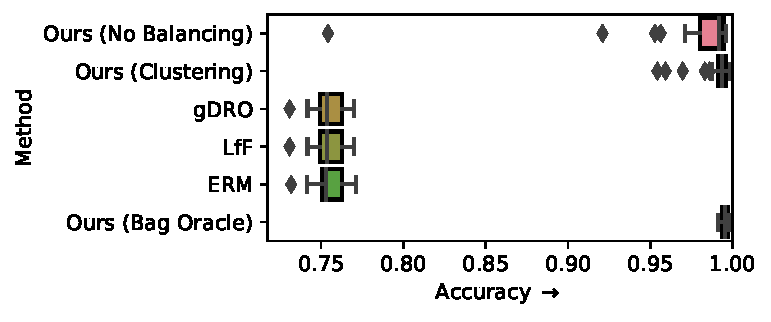
\includegraphics[width=0.49\textwidth]{supmatch/figures/cmnist/subgroup_bias/cmnist_2v4_partial_acc.pdf}
  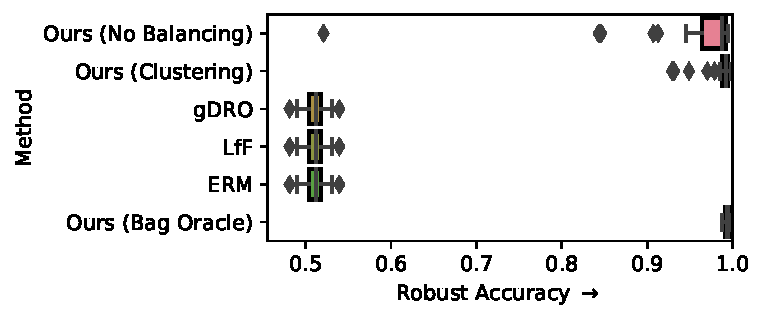
\includegraphics[width=0.49\textwidth]{supmatch/figures/cmnist/subgroup_bias/cmnist_2v4_partial_acc-min.pdf}
%   \includegraphics[width=\columnwidth]{figures/cmnist_2v4_partial_tpr.pdf}
%   \includegraphics[width=\columnwidth]{figures/cmnist_2v4_partial_tnr.pdf}
  \caption{
    Results for the \emph{subgroup-bias} scenario where {\color{purple}purple} fours constitute the missing source.
    %
    The clustering accuracy for \texttt{Ours (No Balancing)} was 96\% $\pm$ 6\%.
    %
    Our method consistently outperforms the baselines, which fare no better than random on the subgroup with the missing source. 
    %
    As we would expect, the median and IQR of our method are positively- and negative- correlated, respectively, with how well the bags of the deployment set are balanced, with \texttt{Ours (Bag Oracle)} providing an upper bound for this.
    %
    Indeed, in one case \texttt{Ours (No Balancing)} failed to outperform the baselines, yet through
    clustering the worst-case \texttt{Robust Accuracy} is limited to within the $95\%$ region.
  }%
  \label{fig:cmnist-2v4-partial}
% \end{figure*}
% \begin{subfigure}
  \end{subfigure}
  
  \begin{subfigure}[b]{\textwidth}
  \centering
  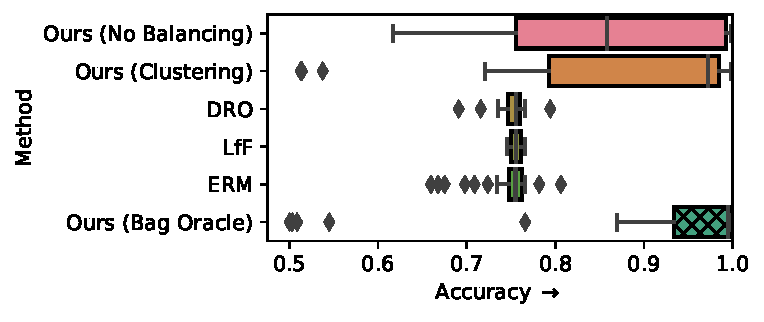
\includegraphics[width=0.49\textwidth]{supmatch/figures/cmnist/missing_subgroup/cmnist_2v4_miss_s_acc.pdf}
  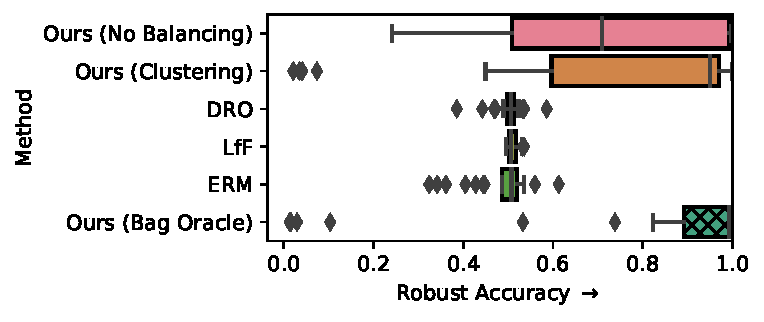
\includegraphics[width=0.49\textwidth]{supmatch/figures/cmnist/missing_subgroup/cmnist_2v4_miss_s_acc-min.pdf}
%   \includegraphics[width=\columnwidth]{supmatch/figures/cmnist_2v4_miss_s_alt_tpr.pdf}
%   \includegraphics[width=\columnwidth]{supmatch/figures/cmnist_2v4_miss_s_alt_tnr.pdf}
  \caption{
    Results for the \emph{missing-subgroup scenario} where {\color{purple}purple} digits constitute the missing subgroup.
    %
    The clustering accuracy for \texttt{Our (No Balancing)} was 88\% $\pm$ 5\%. 
    This scenario is significantly more difficult to solve than the subgroup-bias as there is insufficient inductive bias in the labels and the deployment set for the support matching to be well-posed. 
    %
    This is reflected in the high variance of our method, variance, however, which can be drastically reduced by improving the quality of balancing.
    %
    Nevertheless, all variants of our method perform significantly better than the baselines in terms of the median \texttt{Robust Accuracy}, and the rate at which they produce degenerate solutions (marked by performance worse than \texttt{ERM}'s) relatively low.
    %
  }%
  \label{fig:cmnist-2v4-miss-s}
  \end{subfigure}
  \caption{
  Results for two-digit Colored MNIST for two different scenarios (subgroup bias (Top) and missing subgroup (Bottom)) in the form of box plots of the \texttt{Robust Accuracy} (the minimum accuracy computed over the subgroups) over \textbf{30 repeats}.
  }
\end{figure*}

%
Appendix~\ref{sec:dataset-construction} provides description of the dataset and the settings used
for \( D^{dep} \) and \( D^{tr} \). 
%
Each source is then a combination of digit-class (class label) and colour (subgroup label). 
%
We begin by considering a binary, 2-digit/2-colour, variant of the dataset with $\gY = \{2, 4\}$
and $\gS = \{\text{\color{green}green}, \text{\color{purple}purple}\}$.
(Appendix~\ref{ssec:3-digit-3-color} provides results for 3-digit/3-colour variant.) 
%
For this variant we explore both the SB (subgroup bias) setting and a more extreme \emph{missing
subgroup} setting.
%
To simulate the SB setting, we set \(\gS^{tr}_{ Y=4 }=\{\text{\color{green}{green}}\}\). 
%
In the \emph{missing subgroup} setting, $S=\text{\color{purple}{purple}}$ is missing from
\(\gS^{tr}_{ Y=2 }\) as well, so that all classes only have support in
\(\{\text{\color{green}{green}}\}\).
%
However, for this scenario, the disentangling procedure has more than one possible solution --
apart from the natural solution, it is also possible to consider ($Y=2$,
$S=\text{\color{green}{green}}$) and ($Y=4$, $S=\text{\color{purple}{purple}}$) as forming one
factor in the disentangling, with the other factor comprising the two remaining
$s$-$y$-combinations.
%
Such an ``unnatural'' disentangling (spanning digit class \emph{and} colour) is avoided only by the
tendency of neural networks to prefer simpler solutions (Occam's razor) and in general we cannot
guarantee that this pathological case be avoided based only on the information provided by the
training labels and deployment set.

To establish the effectiveness of our method, we compare against four baselines.
%
The first is \texttt{ERM}, a classifier trained with cross-entropy loss on this data; the second is
\texttt{DRO} \citep{HasSriNamLia18}, which functions without subgroup labels by minimising the
worst-case training loss over all possible groups that are above a certain minimum size; the third
is \texttt{gDRO} \citep{sagawa2019distributionally}, which minimises the worst-case training loss
over predefined subgroups but is only applicable when $|\gS^{tr}| > 1$; the fourth is \texttt{LfF}
\citep{NamChaAhnLeeetal20} which reweights the cross-entropy loss using the predictions of a
purposely-biased sister network.
%
For fair comparison, the training set is balanced according to the rules defined in
\S\ref{sec:sm-adversarialsm} for all baselines.

Fig.~\ref{fig:cmnist-2v4-partial} shows the results for the SB setting. 
%
We see that the performance of our method directly correlates with how balanced the bags are, with
the ranking of the different balancing methods being \texttt{Oracle} $>$ \texttt{Clustering}$>$
\texttt{No Balancing}. 
%
Even without balancing, our method greatly outperforms the baselines, which all perform similarly.

Fig.~\ref{fig:cmnist-2v4-miss-s} shows that the problem of \emph{missing subgroups} is harder to
solve.
%
For all balancing strategies, the IQR is significantly higher than observed in the SB setting, with
the latter also giving rise to a large number of extreme outliers. 
%
The median, however, remains high, indicative of a ``hit-or-miss'' aspect to the method, albeit
with the number of hits far outweighing the misses. 
%
Visualisations of the reconstructions (Appendix~\ref{sec:qual-results})
suggest that the extreme outliers correspond to the degenerate solution mentioned above.
% with $z$ zeroed-out suggests that misses often mostly occurred due to the semantic information
% being concentrated in $\tilde{s}$ while $z$ is left to contain only residual information, even
% when $\tilde{s}$ was set to be one-dimensional and binarized. 
%
% We leave it to future work to explore how to better obviate such degeneracies.

% \begin{figure}[tbp]
%   \centering
%    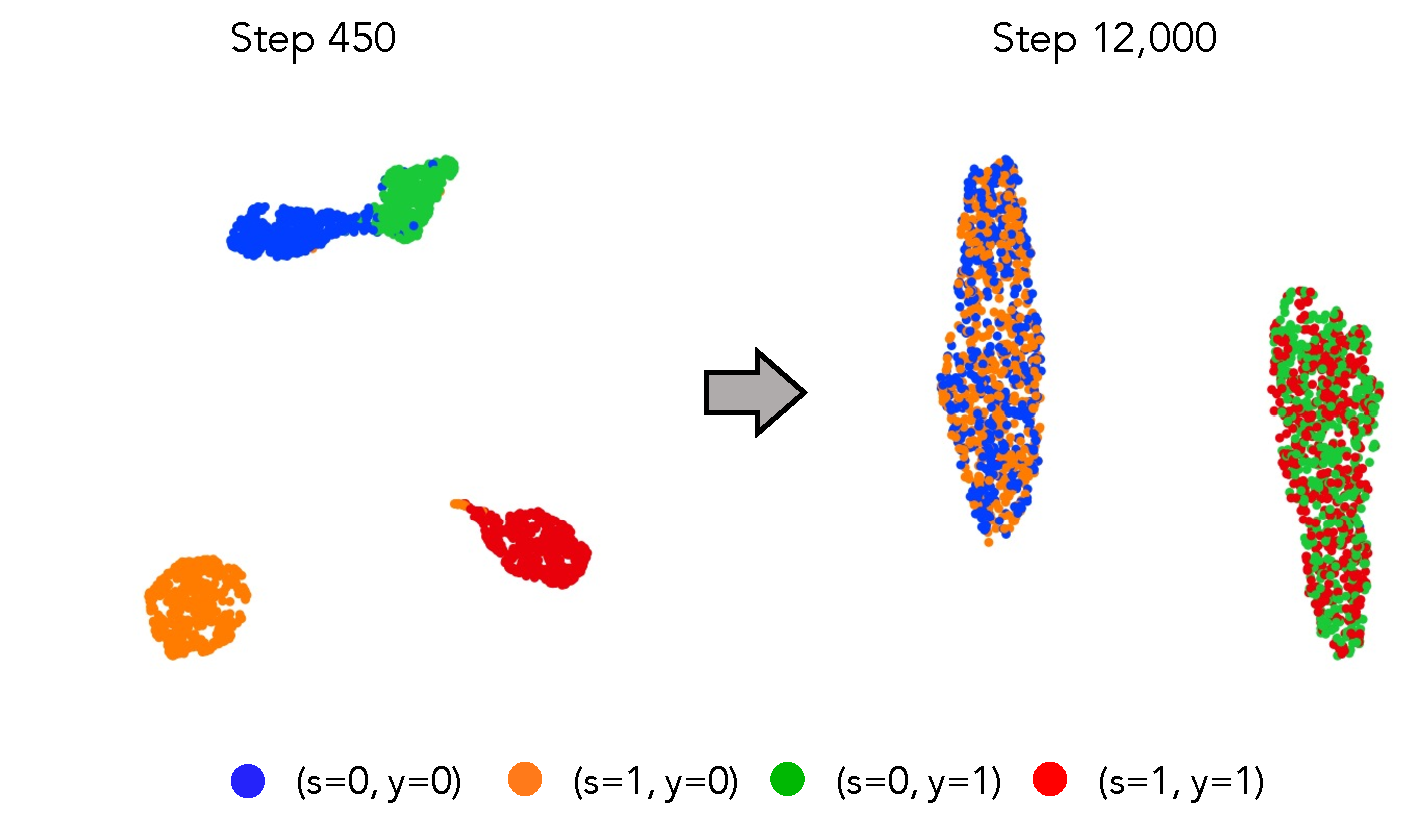
\includegraphics[width=0.6\columnwidth]{supmatch/figures/illustrations/umap_viz.pdf}
%   \caption{%
%     UMAP visualisations of the representations learned by the debiaser for the Colored MNIST
%     dataset. \textbf{Left}: After 450 training-steps each source forms a distinct cluster.
%     \textbf{Right}: After 12,000 training-steps sources with the same $y$-value have merged, thus
%     eliminating the spurious correlation between digit and color.
%   }%
%   \label{fig:umap}
% \end{figure}

% We visualise the learned representation -- from a successful run -- using UMAP
% \citep{mcinnes2018umap} in Fig.~\ref{fig:umap}. % Here, we see that at the beginning of training,
% all four sources are distinct, and the two sources with $s=0$ (from which one is missing in the
% training set) are closer to each other than to their respective classes. % At the end of
% training, the representations clearly separate into two clusters corresponding to the two
% classes, while the subgroups are distributed evenly therein.

\subsection{CelebA}\label{ssec:celeba_exp}
%
\begin{figure*}[t]
  \centering
  % Smiling females missing
%   \normalsize{Missing source: smiling females}\par\medskip
%  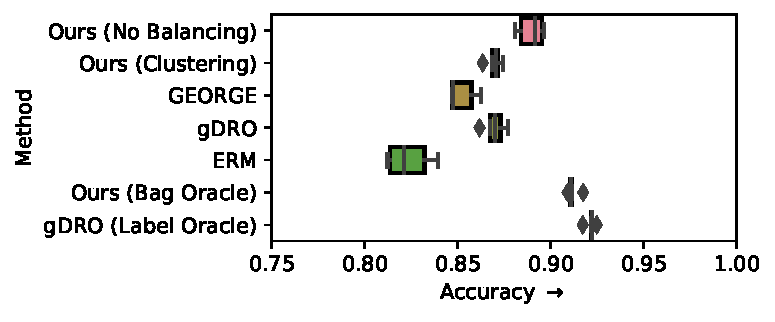
\includegraphics[width=0.49\textwidth, height=3cm]{supmatch/figures/celeba/no_smiling_females/celeba_gender_smiling_acc.pdf}
 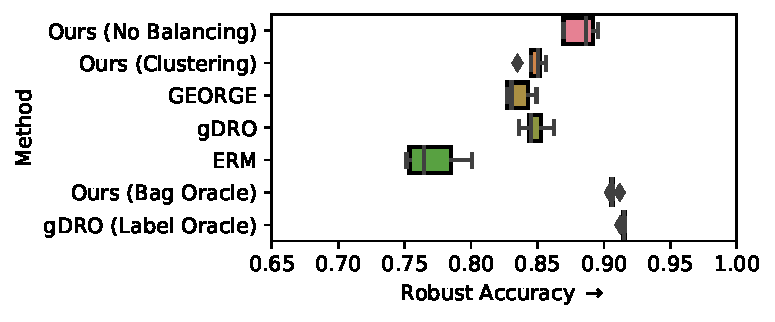
\includegraphics[width=0.49\textwidth]{supmatch/figures/celeba/no_smiling_females/celeba_gender_smiling_acc-min.pdf}
    % Smiling males missing
%   \normalsize{Missing source: smiling males}\par\medskip
%  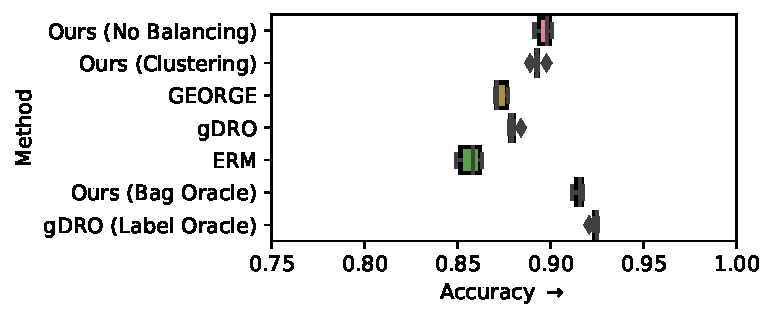
\includegraphics[width=0.49\textwidth]{supmatch/figures/celeba/no_smiling_males/celeba_gender_smiling_acc.pdf}
 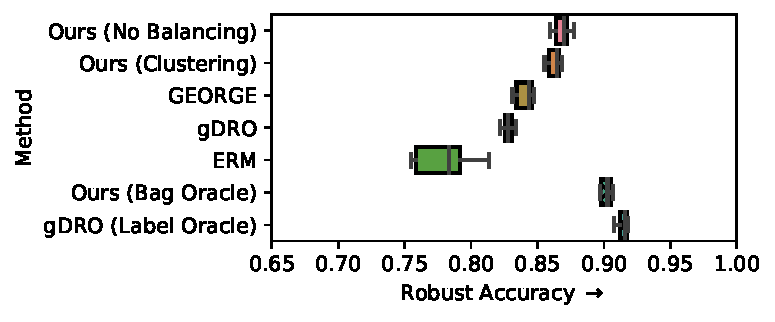
\includegraphics[width=0.49\textwidth]{supmatch/figures/celeba/no_smiling_males/celeba_gender_smiling_acc-min.pdf}
    % Unsmiling females missing
%   \normalsize{Missing source: non-smiling} females\par\medskip
%  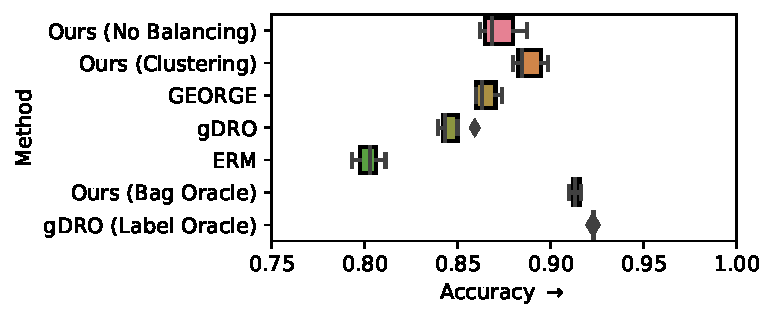
\includegraphics[width=0.49\textwidth]{supmatch/figures/celeba/no_unsmiling_females/celeba_gender_smiling_acc.pdf}
 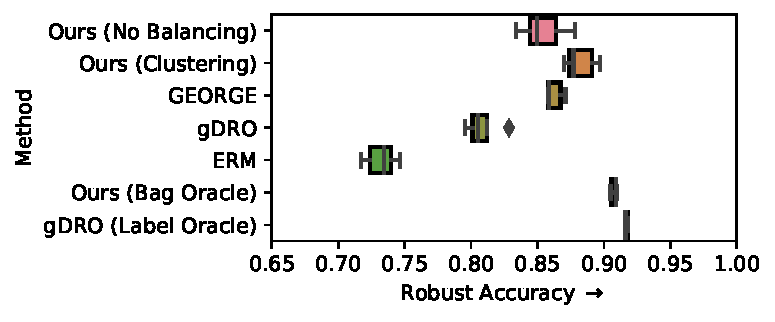
\includegraphics[width=0.49\textwidth]{supmatch/figures/celeba/no_unsmiling_females/celeba_gender_smiling_acc-min.pdf}
  % Unsmiling males missing
%   \normalsize{Missing source: non-smiling males}\par\medskip
%  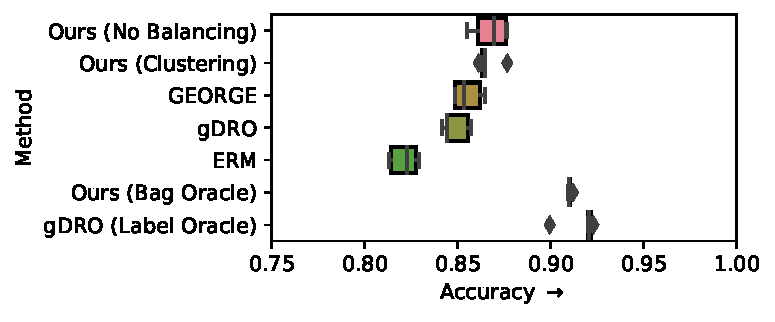
\includegraphics[width=0.49\textwidth]{supmatch/figures/celeba/no_unsmiling_males/celeba_gender_smiling_acc.pdf}
 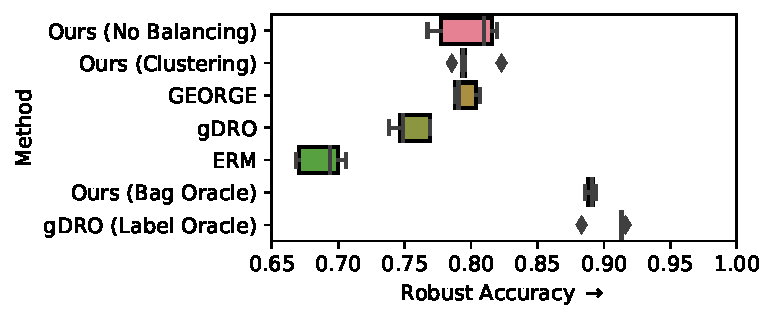
\includegraphics[width=0.49\textwidth]{supmatch/figures/celeba/no_unsmiling_males/celeba_gender_smiling_acc-min.pdf}

% compressed figures:
%   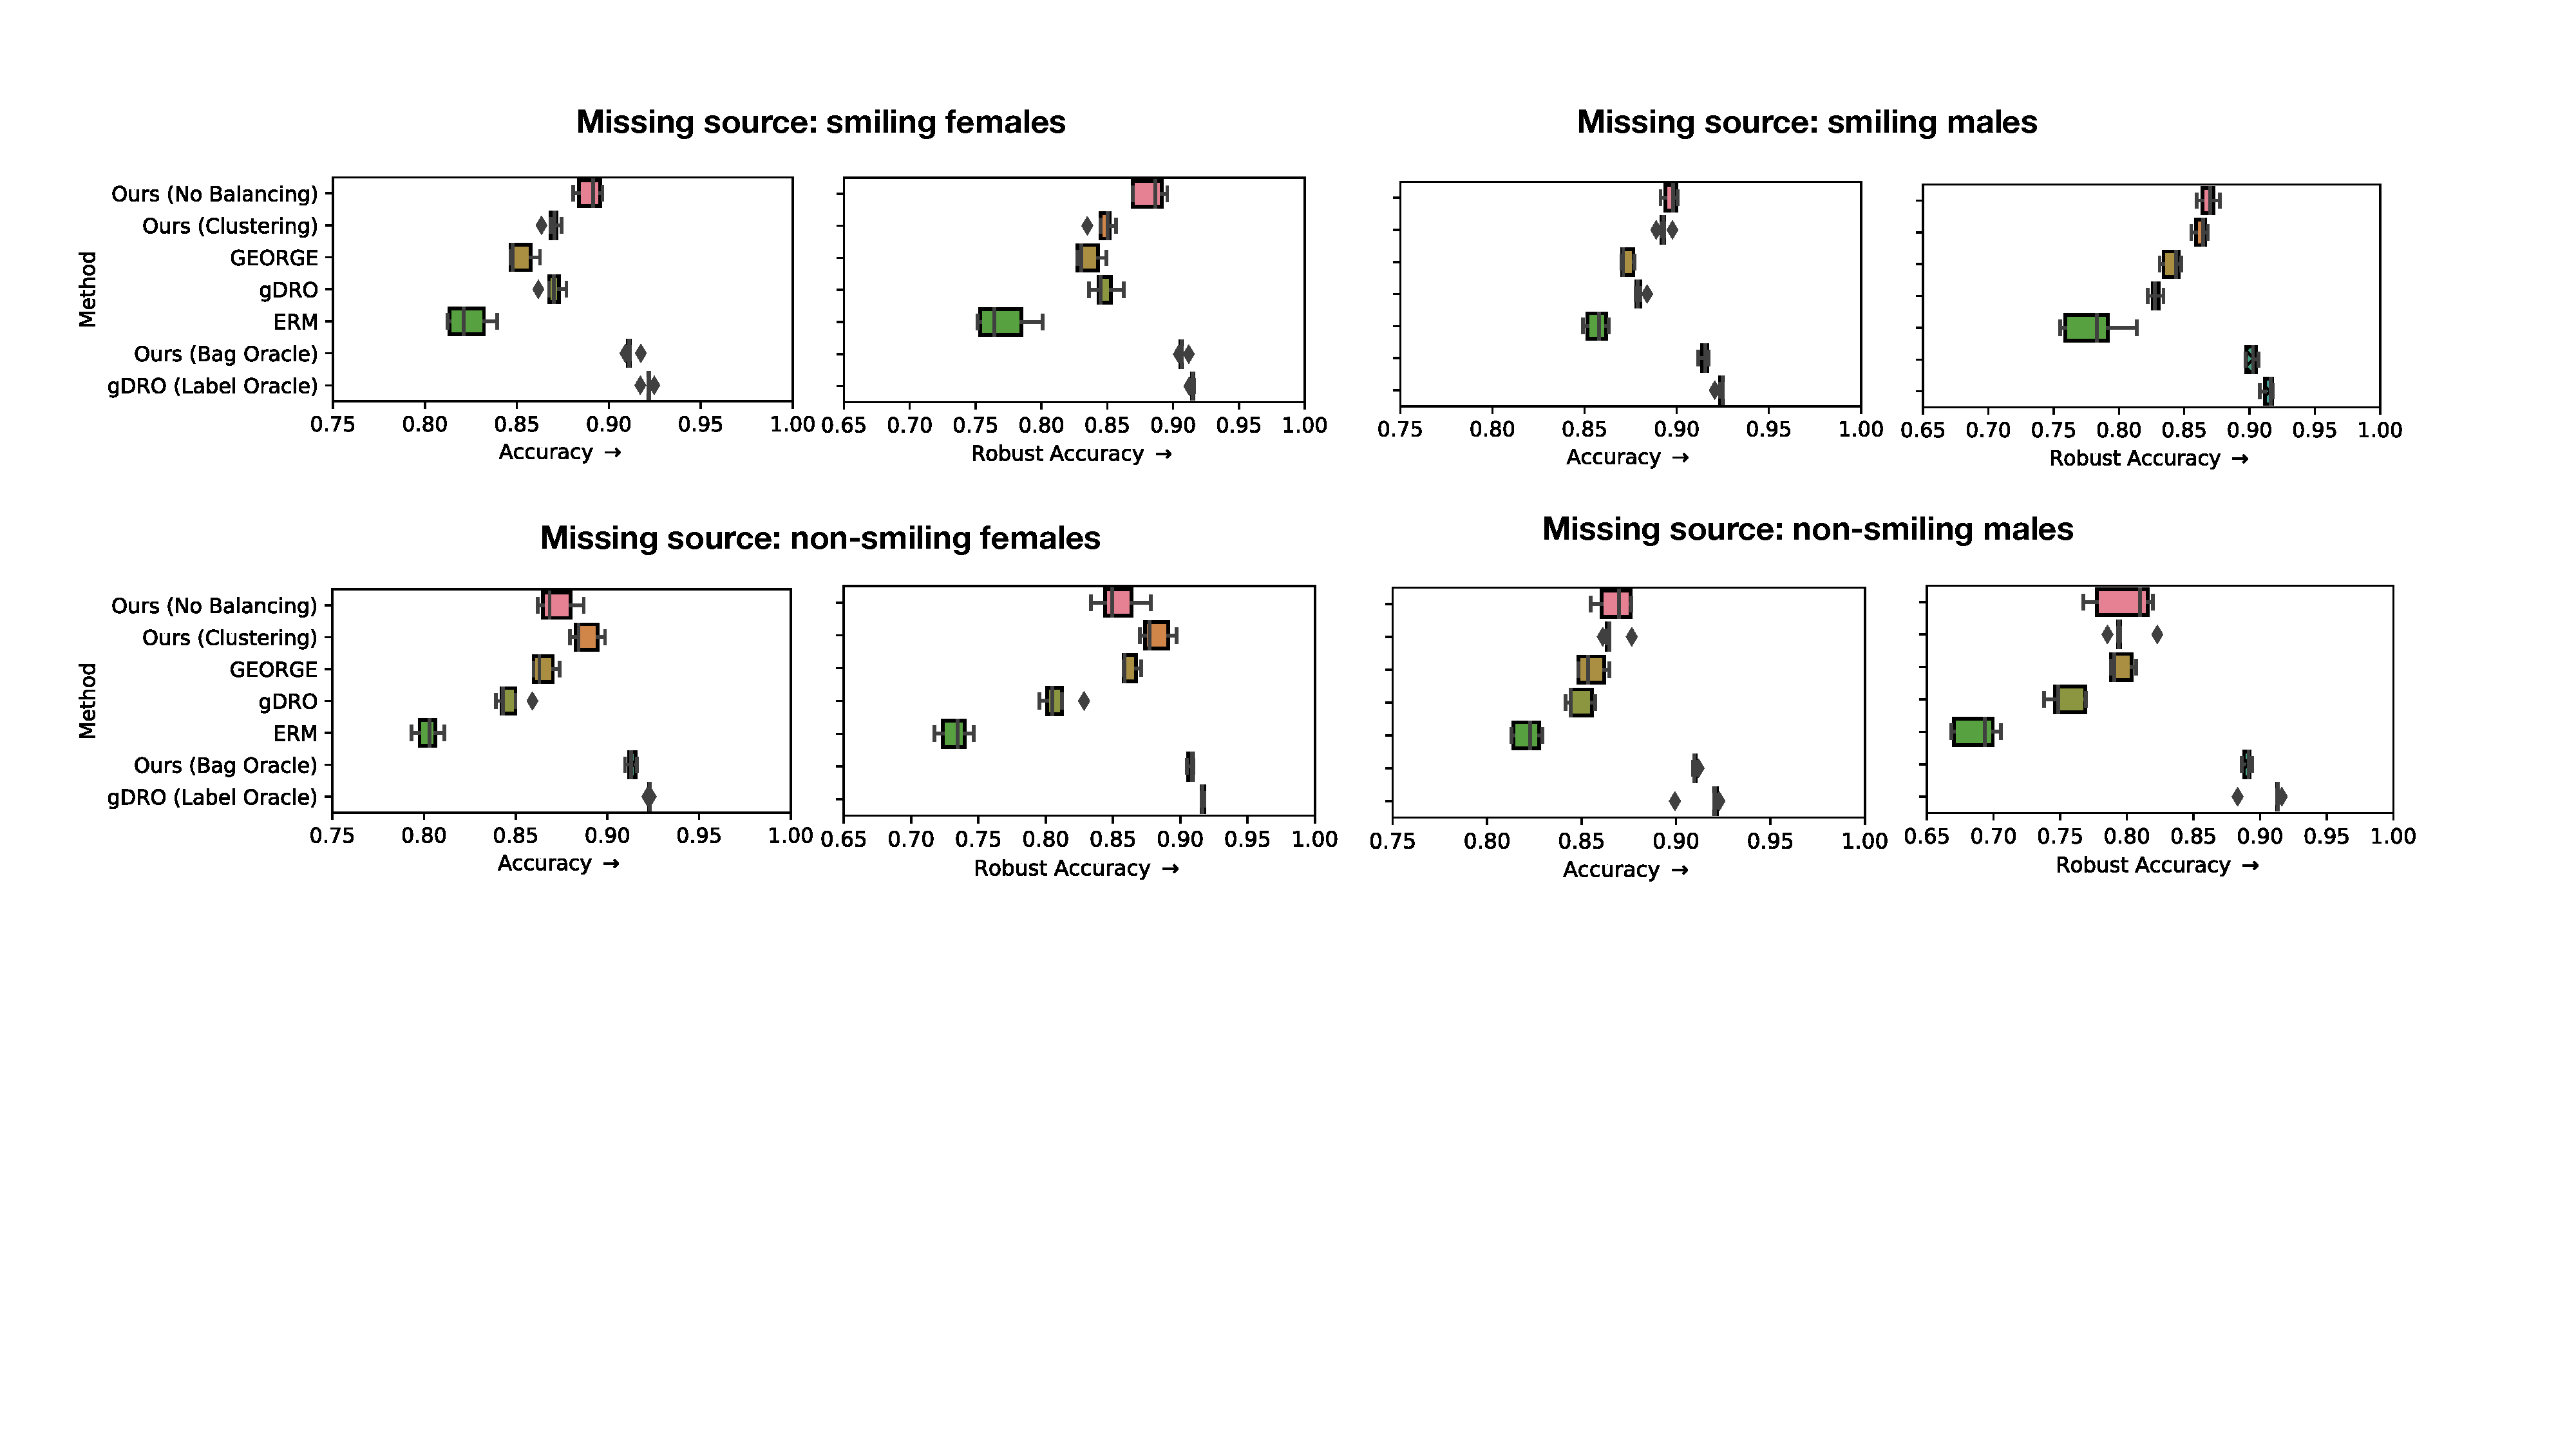
\includegraphics[width=1.0\textwidth]{supmatch/figures/celeba/CelebA2.pdf}
  \caption{
    Results from \textbf{5 repeats} for the CelebA dataset for the \emph{subgroup bias} scenario.
    The task is to predict ``smiling'' vs ``non-smiling'' and the subgroups are based on gender. 
    %
    The four sources are dropped one at a time from the training set
    (\textbf{Top Left}: smiling females; \textbf{Top Right}: smiling males; \textbf{Bottom Left}: non-smiling females;
    \textbf{Bottom Right}: non-smiling males), while the deployment set is kept fixed.
    %
    \texttt{Robust Accuracy} refers to the minimum accuracy computed over the subgroups.
    %
    Our method consistently performs on par with or outperforms \texttt{GEORGE} (which in turn outperforms \texttt{ERM}).
    %
    We note that in some of the runs, \texttt{GEORGE} performed no better than random -- these results were truncated for visibility but can be found in
    Fig.~\ref{fig:celeba-gender-smiling-full}.
    %
    % Due to poor clustering accuracy and the fact that the deployment set is naturally relatively well-balanced with respect to gender, \texttt{Ours (Clustering)} failed to improve on \texttt{Ours (No Balancing)} for all but one missing source.
    %
    Given \emph{indirect} supervision from the deployment set in the form of oracle-balancing, our method performs similarly to \texttt{gDro (Label Oracle)} that receives \emph{direct} supervision.
  }%
  \label{fig:celeba-gender-smiling}
\end{figure*}


%
To demonstrate our method generalises to real-world computer vision problems, we consider the
CelebA dataset~\citep{liu2015celeba} comprising over 200,000 images of different celebrities. The
dataset comes with per-image annotations of physical and affective attributes such as `Smiling',
`Gender', hair colour, and `Age'.
%
Since the dataset exhibits natural imbalance with respect to $\gG$, we perform no additional
sub-sampling of either the training set or the deployment set. We predict ``smiling'' as the class
label and use the binary attribute, ``gender'', as the subgroup label. Here, we consider the SB
setting but rather than just designating one missing source, we repeat our experiments with each
source being dropped in turn.
%
As before, we evaluate our method under three balancing schemes and compare with ERM and gDRO
trained on only the labelled training data.
%
We also compare with two other variants of gDRO: 1) \texttt{gDRO (Label Oracle)}, a variant that is
trained with access to the ground-truth labels of the deployment set, thus providing an upper-bound
on the downstream classification performance; 2) \texttt{GEORGE} \citep{SohDunAngGuetal20}, which
follows a two-step procedure of first clustering to obtain the labels for hidden subgroups, and
then using these labels to train a robust classifier using gDRO.
%
\citet{SohDunAngGuetal20} consider a different version of the problem (termed
\emph{hidden-stratification}) in which the class labels are known for all samples but the
subgroup-labels are missing entirely.
%
We adapt \texttt{GEORGE} to our setting by modifying the semi-supervised clustering algorithm to
predict the marginal distributions (\(P(Y|X)\) and \(P(S|X)\) instead of the joint distribution
\(P(Y, S|X)\), allowing us to propagate the class labels from \( D^{tr} \) to \( D^{dep} \) (see
Appendix~\ref{adapting_g} for details).
% Following this, gDRO is trained on the combination of the training and deployment sets, with the
% latter's labels conferred by clustering.


Fig.~\ref{fig:celeba-gender-smiling} shows the results for experiments for each missing source,
showing similar trends across all instantiations of the SB scenario. 
%
\texttt{gDRO (Label Oracle)} consistently achieves the best performance according to both metrics,
with \texttt{Our Method (Bag Oracle)} consistently coming in second. 
%
We note that while both methods use some kind of oracle, the \emph{label oracle} provides
\emph{all} class/subgroup labels to its algorithm, whereas the \emph{bag oracle} only balances the
bags. 
%
Despite the large difference in the level of supervision, the margin between the two oracle methods
is slim. 
%
We observe that clustering in many cases impairs performance which can be explained by poor
clustering of the missing source ($\sim$60\% accuracy).
%
CelebA exhibits a natural imbalance with respect to gender/smiling but not a significant one,
allowing for random sampling to yield a reasonable approximation to the desired perfect bags. 
%
We believe adjustments to the clustering algorithm -- e.g.\ using a self-supervised loss instead of
a reconstruction loss for the encoder -- could close the gap between clustering-based and
oracle-based balancing. 
%
Nonetheless, among the non-oracle methods, variants of our method
consistently match or exceed the performance of the baselines. 
%
While the plots show \texttt{GEORGE} can perform strongly in this SB scenario, we note that for
several of the missing sources, the method failed catastrophically in one out of the five runs.
%
We have cut off those data points here so as not to compromise the visibility of the other results;
the full versions of the plots can be found in Appendix~\ref{ssec:extended-results-celeba}.
%
The fact that \texttt{GEORGE} leverages both the training and deployment sets in a semi-supervised
way with clustering makes it the baseline most comparable to our method.
%
However, its performance is much more dependent on the clustering step than our method.

% %
% \subsection{Chest-Xray8}{\label{ssec:nih_exp}}
% %
% The Chest-Xray8 dataset \citep{wang2017chestx}  comprises 108,948 frontal-view X-ray images with
% weak labels -- mined automatically from radiology reports using natural language processing --
% indicating positive diagnosis of eight thoracic diseases. 
% %
% These labels are mutually inclusive and as such give rise to a multi-label classification task. 
% %
% Among the images, 24,636 are associated with one or more pathologies, while the remaining 84,312
% are derived from healthy patients.
% % Atelectasis, Cardiomegaly, Effusion, Infiltration, Mass, Nodules, Pneumonia, Pneumothorax
% To simplify the analysis, we convert the problem into one of binary classification by considering
% only he most frequently occurring pathology, ``infiltration''. 
% %
% We note that, since our method only uses the target implicitly via balancing in order to learn
% invariance to the subgroup, and this objective is balanced with the goal of maximally preserving
% information about the input, \( \gI(f(X);X) \), rather than the target directly, the resulting
% representation could be can be used for any of the targets without detriment. 
% %
% We designate ``gender'' as the subgroup label, following \citep{seyyed2020chexclusion}, and
% simulate the SB setting by dropping from the training set male patients with a positive diagnosis,
% i.e. by setting \(\gS^{tr}_{ Y=\text{infiltration} }=\{\text{female}\}\).


% \subsection{Sensitivity Analysis}\label{ssec:sensitivity}

% To assess the empirical robustness of our algorithm to noise in the bag-balancing, we conduct an
% sensitivity analysis using the Chest-Xray8 dataset. 
% %
% Using the same configuration used to collect the results from the previous section, we run our
% algorithm with the ground-truth labels used for balancing but with \( \{5\%, 10\%, \dots, 50\%\} \)
% of the labels perturbed (flipped). 
% %
% Rather than randomly perturbing the labels by sampling from the set of complementary labels --
% i.e., \( \tilde{g}_i \sim \mathrm{uniform}(\gG \setminus \{g_i\}) \), with \( g_i \) and \(
% \tilde{g}_i \) denoting the ground-truth and the perturbed labels, respectively -- which yields
% unrealistic perturbations due to the discounting the semantic relationships between groups
% (semantically similar groups are more likely to be confused by a clustering algorithm) we instead
% sample a perturbed label, $\tilde{g}_i$ from $\gG$ with probability proportional to the similarity
% between the associated (featurised) sample and the \(\tilde{g}_i\)th centroid, \(
% \phi_{\tilde{g}_i} \in \mathbb{R}^d \), with the constraint that the perturbed label does not equal
% the original one. 
% %
% This is done using features extracted by a pre-trained CLIP \citep{radford2021learning} visual
% encoder. Namely, the centroids \( \Phi \in \mathbb{R}^{|\gG| \times d} \) are computed as the
% group-conditional means of these features, over the deployment set, and their similarity with a
% given sample's features is measured using cosine similarity. 
% %
% Assuming \(L_2\)-normalised CLIP features, $\bar z_i^\text{CLIP} \in \mathbb{R}^d$, and prototypes,
% $\bar \Phi$, the sampling scheme used to generate the perturbed label, $\tilde{g}_i$, for a given
% ground-truth label, $g_i$, can be written as
% %
% \begin{align}
%   %
%   \tilde{g}_i \sim \text{Cat}(\gG, \bigtriangleup_\mathbf{w} ), \quad
%   %
%   \bigtriangleup_\mathbf{w} \triangleq  \frac{\mathbf{w}}{\sum_j \mathbf{w}_j} , \quad
%   %
%   \mathbf{w} \triangleq \text{exp}(\bar z_i^\text{CLIP} \cdot \bar \Phi \tau^{-1})
%   \odot (1 - e_{g_i}),
%   %
% \end{align}
% %
% where \( \text{Cat} \) denotes the categorical distribution with support \(\gG\) and sampling
% probabilities \( \bigtriangleup_w \), \( \tau \in \mathbb{R}^+_\ast \) denotes a temperature
% parameter modulating the sharpness of the sampling distribution, \(e_{g_i}\) denotes the one-hot
% encoding of \(g_i\), and \(\odot\) denotes the Hadamard product that is used with \(e_{g_i}\) to
% mask out the \(g_i\)th prototype and thereby enforce \( \tilde{g}_i \neq g_i \).

% which shows strong performance even without balancing.

% Now that we have them, we can discuss the results with clustering.
%
% We did not use the clustering approach for CelebA, as the attributes ``smiling'' and ``gender''
% are not the most salient; more work is needed on the clustering side to discover all semantically
% meaningful clusters.
%
% Nonetheless, our method consistently outperforms the baselines even when no balancing is applied
% Furthermore, we show qualitative results of the disentangling in fig.~\ref{fig:celeba-recons},
% and note a clear separation of subgroup-relevant information from subgroup-irrelevant
% information.
%in $g(0, f_s(x))$ and $g(f(x), 0)$, respectively.

%Furthermore, we control the \emph{number of clusters},which means all samples can get sorted into
%the right \emph{number of groups}. 
%
% Instead we use the idea of balanced dataset and sample equal amount of samples from each cluster
% to form a batch. 
  
% \textbf{Disentangled representations via adversarial autoencoders}
%We want to learn a disentanglement using a perfect dataset as the supervision signal.
%
%To achieve this, our semi-supervised disentanglement learning framework (fig.
%\ref{fig:architecture} ) maps data points into independent factors of variations such that our
%training dataset $D_{\text{tr}}$ and our deployment set $D_c$ are indistinguishable; i.e., we
%would like transform $D_{\text{tr}}$ such that the independence condition $y\perp s$ holds.
%
%However, the deployment set itself $D_c$ might not amount to a suitable target distribution in
%which the independence condition holds.
%
%The idea is to make the deployment set $D_c$ approximately perfect by balancing it according to
%the cluster IDs, forming the set $D_p$.
%
% We create disentangled representations by training four separate neural networks, which we denote
% $f$, $g$, $h$ and $l$. % We use mean squared error for the reconstruction loss, and the binary
% cross entropy error for the discriminator loss. % For a dataset with mixed-typed attributes, we
% use a combination of mean squared error and (binary) cross entropy error for the reconstruction
% loss. % We optimize the proposed model using a scheduled update scheme where we freeze the
% weights of the autoencoder and predictor modules when we update the weights of the discriminator,
% and vice versa.
%



\section{Related work}
\label{sec:sm-related-work}
\paragraph{Invariant learning}
\citet{SohDunAngGuetal20} and \citet{creager2021environment} both consider a similar problem, where
the data also exhibits a two-level hierarchy formed by classes and subgroups.
%
In contrast to our work, however, there is no additional bias in the data; while they may be
unobserved, the labelled data is assumed to have complete class-conditional support over the
subgroups.
%
As such, these methods are not directly applicable to the particular form of the problem we
consider.
%
Like us, \citet{SohDunAngGuetal20} uses semi-supervised clustering to uncover the hidden subgroups,
however their particular clustering method requires access to the class labels not afforded by the
deployment set, as does the training of the robust classifier.

\paragraph{Unsupervised domain adaptation}
In unsupervised domain adaptation (UDA), there are typically one or more source domains, for which
training labels are available, and one or more unlabelled target domains to which we hope to
generalise the classifier.
%
A popular approach for solving this problem is to learn a representation that is invariant to the
domain using adversarial networks \citep{ganin2016domain} or non-parametric discrepancy measures
such as MMD \citep{gretton2012kernel}.
%

There are two ways in which one can compare UDA to our setting: 1) by treating the subgroups as
domains; and 2) by treating the training and the deployment set as ``source'' and ``target''
domains, respectively.
%
The first comparison is exploited in algorithm fairness, yet does not carry over to our setting in
which the labelled data contains \emph{incomplete} domains. 
%
When all sources from a given domain are missing then there are no domains to be matched, and even
when this is not the case, matching will result in misalignment due to differences in
class-conditional support.
%
The second comparison is more germane but ignores an important aspect of our problem: the presence
of spurious correlations.
%

Similar to us, \citet{tong2022adversarial} utilise adversarial methods to align the support of two
distributions in a semi-supervised regime -- specifically, they propose to use symmetric support
difference as a divergence measure which they realise using a discriminator. 
However, their method focuses on label-shift in the UDA
setting and does not consider the hierarchical structure that exists within the source (training)
and target (deployment) domains, and as such they do not consider the notion of ``missing sources''
that can arise due to said structure -- the characterisation of this problem is one of the two
main contributions of this work (the other being our proposed solution). Furthermore, the
discriminator used therein is applied instance-wise; we show in \ref{sec:ablations} that allowing
the discriminator to model inter-sample relationships has tangible addition benefits when
performing support-matching.

\paragraph{Multiple instance learning}
Multiple instance learning \citep{maron1998framework} is a form of weakly-supervised learning in
which samples are not labelled individually part as part of a set or \emph{bag} of samples.
%
In the simplest (binary) case, a bag is labelled as positive if there is a single instance of a
positive class contained within it, and negative otherwise.
%
In our case, we can view the missing sources as constituting the positive classes, which leads to
all bags (a term we will use throughout the paper distinctly from ``batches'') from the deployment
set being labelled as positive, and all bags from the training set being labelled as negative.
%
Given this labelling scheme, we make use of an adversarial set-classifier to align the supports of
the training and deployment sets in the representation space of an encoder network.
%

\paragraph{Positive unlabelled learning}
Learning from positive and unlabelled data, or \emph{PU learning}, refers to the
binary-classification setup in which the labelled training data consists of only positive samples
while additional unlabelled data is assumed to contain both positive and negative samples
\citep{liu2002partially, liu2003building, bekker2020learning}. This is analogous to our problem
setting if we consider the positive class to be all samples sources represented in the training
set, collectively, while the missing sources collectively make up the negative class. However, the
goal here is not merely to learn the classification boundary between the present and missing
sources but to learn to classify the target class of a given sample independently of its subgroup.
This is equivalent to requiring that a classifier trained to distinguish between positive and
negative classes, according to the aforementioned PU learning setup, from the pre-logits layer of
our desired classifier be maximally entropic -- we propose to use adversarial learning to achieve
this.

% \paragraph{Fairness}


\section{Conclusion and ongoing work}
\label{sec:sm-conclusion}
%
\corr{
  %
In this paper, we formalised the problem that systematic bias or dataset curation resulting in one or more
subgroups having zero labelled data; we hope our doing so stimulates serious consideration
for it in the planning, building, and evaluating systems.
%
This complements concurrent research by \citet{yang2023change} wherein the same problem (with
different formalism) is alluded to, but its solution left as an open question.
%
Contrastingly, we proposed here a two-step approach for addressing the problem within a
semi-supervised framework. 
%
The first step entails constructing hierarchically-balanced bags from an unlabelled deployment set
via one's semi-supervised clustering algorithm of choice.
%
The second step then entails matching the support, instead of the raw distributions, of the
training and deployment sets in representation space, so as to learn subgroup-invariant
representations, an outcome we prove corresponds to the optimum of the proposed objective function.
%
We empirically validate our frame\-work on the Coloured MNIST and CelebA datasets, showing it
possible to maintain high performance on subgroups with incomplete support.
%
Furthermore, we bound the error in the objective incurred due to imperfect clustering and show that
the proposed set-wise discriminator is empirically more robust to this error than conventional
instance-wise discriminators.
%
Future work includes the exploration of other \ac{UL} methods for realising the \ac{MI} component
of the objective and addressing the limitations raised in \S\ref{sec:sm-limitations}.

\subsection{Dataset representativity}
%
The results presented in this version of the paper are for toy (Coloured MNIST) or pseudo-toy
(CelebA) datasets; though both datasets have featured extensively in the literature on
distributional-robust learning (\citealp{arjovsky2019invariant, kim2019learning,
sagawa2019distributionally, creager2021environment}, inter alia) it is natural to doubt the
representativeness of results on them in relation to real-world problems.  
%
To shore up this shortcoming, we have since conducted experiments with two datasets more emblematic
of real-world realisations of the proposed problem, namely Chest-Xray8 \citep{wang2017chestx} and NICO++
\citep{zhang2023nico++}.
%
The former dataset is appealing as it coincides with the motivating example proffered in
\S\ref{sec:sm-intro}; the latter is so as its class-subgroup structure allows for demonstration in
a non-binary (\wrt{} both marginals) setting, whereas the results contained herein were
preponderantly binary out of both simplicity and convention.
%

\subsection{Sensitivity analysis \wrt{} bag-balancing}
%
As noted, we provided bounds on the error in alignment propagated by the error in
approximating \( \gD^{dep}\) but empirical analysis of the reification of this is lacking. 
%
Accordingly, we have sought to effect this via controlled sensitivity analyses \wrt{} the
balancing.
To achieve this, we run our support-matching algorithm with ground-truth labels used for balancing
but with different proportions (typically \( \{5\%, 10\%, \dots, 50\%\} \)) of said labels
perturbed (flipped or randomly shifted cyclically). 
%
Rather than randomly (uniformly) perturbing the labels by sampling from the set of complementary
labels -- i.e., \( \tilde{g}_i \sim \mathrm{uniform}(\gG \setminus \{g_i\}) \), with \( g_i \) and
\( \tilde{g}_i \) denoting the ground-truth and the perturbed labels, respectively -- which yields
unrealistic perturbations due to the discounting of semantic relationships between groups
(semantically similar groups are more likely to be confused by a clustering algorithm) we instead
sample a perturbed label, $\tilde{g}_i$ from $\gG$ with probability proportional to the similarity
between the featurisation of the associated sample and the \(\tilde{g}_i\)th centroid, \(
\phi_{\tilde{g}_i} \in \mathbb{R}^d \), with the constraint that the perturbed label does not equal
the original one. 

%
The featurisation is performed using a pre-trained (via contrastive captioning) CLIP
\citep{radford2021learning} visual encoder. 
%
Namely, the centroids \( \Phi \in \mathbb{R}^{|\gG| \times d} \) are computed as the
group-conditional means of these features, over the deployment set, and their similarity with a
given sample's features is measured using cosine similarity. 
%
Assuming \(L_2\)-normalised CLIP features, $\bar z_i^\text{CLIP} \in \mathbb{R}^d$, and prototypes,
$\bar \Phi$, the sampling scheme used to generate the perturbed label, $\tilde{g}_i$, for a given
ground-truth label, $g_i$, can be written as
%
\begin{align}
  %
  \tilde{g}_i \sim \text{Cat}(\gG, \bigtriangleup_\mathbf{w} ), \quad
  %
  \bigtriangleup_\mathbf{w} \triangleq  \frac{\mathbf{w}}{\sum_j \mathbf{w}_j} , \quad
  %
  \mathbf{w} \triangleq \text{exp}(\bar z_i^\text{CLIP} \cdot \bar \Phi \tau^{-1})
  \odot (1 - e_{g_i}),
  %
\end{align}
%
where \( \text{Cat} \) denotes the categorical distribution with support \(\gG\) and sampling
probabilities \( \bigtriangleup_w \), \( \tau \in \mathbb{R}^+_\ast \) denotes a temperature
parameter modulating the sharpness of the sampling distribution, \(e_{g_i}\) denotes the one-hot
encoding of \(g_i\), and \(\odot\) denotes the Hadamard product that is used with \(e_{g_i}\) to
mask out the \(g_i\)th prototype and thereby enforce \( \tilde{g}_i \neq g_i \).
%
% CORRECTED: Include any work that you have done since.
}



% \section*{Acknowledgements}
% \label{sec:sm-ack}
% % This research was supported in part by a European Research Council (ERC) Starting Grant for the project ``Bayesian Models and Algorithms for Fairness and Transparency'',
% funded under the European
% Union's Horizon 2020 Framework Programme
% (grant agreement no. 851538).
% Novi Quadrianto is also supported by the Basque Government
% through the BERC 2018-2021 program and by Spanish Ministry of Sciences, Innovation and Universities:
% BCAM Severo Ochoa accreditation SEV-2017-0718.


\newpage
% \section{Additional experiments}\label{sec:additional-results}
% \subsection{Results for Adult Income}\label{sec:adult-results}
% \begin{figure*}[htp]
%     \centering
%     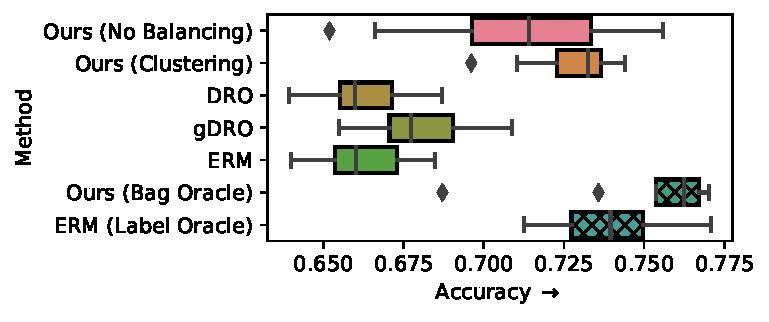
\includegraphics[width=0.49\textwidth]{supmatch/figures/adult/subgroup_bias/adult_partial_acc.pdf}
%     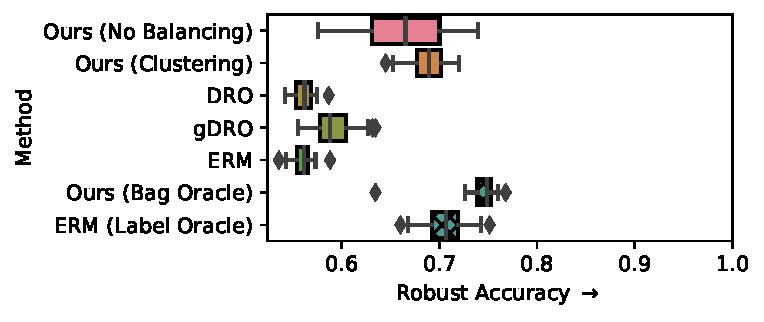
\includegraphics[width=0.49\textwidth]{supmatch/figures/adult/subgroup_bias/adult_partial_acc-min.pdf}
%     \includegraphics[width=0.49\textwidth]{supmatch/figures/adult/subgroup_bias/adult_partial_tprr.pdf}
%     \includegraphics[width=0.49\textwidth]{supmatch/figures/adult/subgroup_bias/adult_partial_tnrr.pdf}
%     \caption{%
%     Results for the Adult Income dataset with \emph{subgroup bias}, for the binary classification
%     task of predicting whether an individual earns $>$\$50,000 with a binary subgrouping based on
%     \emph{gender}. \texttt{ERM (Label Oracle)} refers to a model based on ERM (empirical risk
%     minimization), trained on a labeled deployment set and as such not suffering from bias
%     present in the training set.
%     \textbf{Top left}: Accuracy.
%     \textbf{Top right}: Robust Accuracy.
%     \textbf{Bottom left}: True positive rate ratio.
%     \textbf{Bottom right}: True negative rate ratio.
%     For \texttt{Ours (Clustering)}, the clustering accuracy was 69.7\% $\pm$ 0.3\%;
%     % for \texttt{K-means} it was 43\% $\pm$ 3\%.
%     }%
%     \label{fig:adult-subgroup-bias}
% \end{figure*}
% \begin{figure*}[htp]
%     \centering
%     \includegraphics[width=0.49\textwidth]{supmatch/figures/adult/missing_subgroup/adult_miss_s_acc.pdf}
%     \includegraphics[width=0.49\textwidth]{supmatch/figures/adult/missing_subgroup/adult_miss_s_acc-min.pdf}
%     \includegraphics[width=0.49\textwidth]{supmatch/figures/adult/missing_subgroup/adult_miss_s_tprr.pdf}
%     \includegraphics[width=0.49\textwidth]{supmatch/figures/adult/missing_subgroup/adult_miss_s_tnrr.pdf}
%     \caption{%
%     Results for the Adult Income dataset with a \emph{missing subgroup}, for the binary
%     classification task of predicting whether an individual earns $>$\$50,000 with a binary
%     subgrouping based on \emph{gender}.
%     \texttt{ERM (Label Oracle)} refers to a model based on ERM (empirical risk minimization),
%     trained on a \textbf{l}abeled \textbf{d}eployment set; thus not suffering from bias in the training set.
%     \textbf{Top left}: Accuracy.
%     \textbf{Top right}: Robust Accuracy.
%     \textbf{Bottom left}: True positive rate ratio.
%     \textbf{Bottom right}: True negative rate ratio.
%     For\texttt{Ours (Clustering)}, the clustering accuracy was 60.4\% $\pm$ 0.8\%.
%     % for \texttt{K-means} it was 44\% $\pm$ 3\%.
%     }%
%     \label{fig:adult-missing-subgroup}
% \end{figure*}
% Figures~\ref{fig:adult-subgroup-bias} and \ref{fig:adult-missing-subgroup} show results from our
% method on the Adult Income dataset \cite{Dua:2017}. This dataset is a common dataset for
% evaluating fair machine learning models. Each instance in the dataset is described by $14$
% characteristics including gender, education, marital status, number of work hours per week among
% others, along with a label denoting income level ($\geq$\$50K or not). We transform the
% representation into $62$ real and binary features along with the subgroup label $s$.
% %%%%%%%%CHECK THESE VALUES%%%%%%%%%%%% The dataset is naturally imbalanced with respect to
% gender: 30\% of the males are labeled as earning more than \$50K per year (high income), while
% only 11\% of females are labeled as such. For further details on the dataset construction, see
% section~\ref{ssec:dataset-construction-adult}. % Following standard practice in algorithmic
% fairness  e.g. \cite{ZemeWuSwePitetal13}, we consider gender to be the subgroup label $s$. % A
% \emph{source} is defined as certain combinations of the subgroup, $s$, and target class, $y$.

% For the Adult Income dataset, we study the following two settings of missing sources, a subgroup
% bias setting and a more extreme missing subgroup setting: 1) \emph{subgroup bias}: we have
% labeled training data for males ($s=1$) with both positive and negative outcomes, but for the
% group of females ($s=0$), we only observe the one-sided negative outcome:
% \(\mathcal{S}_{tr}(y=1)=\{1\}\); 2) \emph{missing subgroup}: we have training data for males with
% positive and negative outcomes, but do not have labeled data for females, i.e.\
% \(\mathcal{S}_{tr}(y=0)=\{1\}\) and \(\mathcal{S}_{tr}(y=1)=\{1\}\).

% As before, \texttt{Ours (Clustering)}, \texttt{Ours (No Balancing)}\ and \texttt{Ours (Bag
% Oracle)} denote variants of our method with different deployment-set balancing strategies. As
% baseline methods, we have \texttt{ERM} (standard empirical risk minimization with balanced
% batches), \texttt{DRO} \cite{HasSriNamLia18}, \texttt{gDRO} \cite{sagawa2019distributionally} and
% \texttt{ERM (Label Oracle)} which is the same model as \texttt{ERM}, but trained with access to
% the ground-truth labels of the deployment set.

% In both settings, we observe the same order as for the other dataset in terms of accuracy:
% \texttt{Ours (Bag Oracle)} achieves the highest performance, followed by \texttt{Ours
% (Clustering)}, then \texttt{Ours (No Balancing)}. However, for the \emph{missing subgroup}
% setting, \texttt{Ours (Clustering)} and \texttt{Ours (Bag Oracle)} perform almost identically,
% with the former outstripping the latter slightly in terms of de-biasing metrics. This reduced
% reliance on balancing can be explained by the additional supervision that comes with having two
% sources missing instead of one -- in order for the discriminator to distinguish between bags from
% the deployment set and bags from the training set, the former need only contain \emph{one} of the
% two missing sources.

% Generally, we observe a high variance in the results. This is not attributable to our method,
% however, with the baselines exhibiting the same behavior, but rather to the fact that the Adult
% Income dataset is a very noisy dataset which, at the best of times, allows only about 85\%
% accuracy to be attained (see also \cite{agrawal2020debiasing}). The problem is that samples vary
% widely in how informative they are. This, coupled with us artificially biasing the dataset to be
% even more biased (as \emph{subgroup bias} and \emph{missing subgroup}), makes the attainable
% performance very dependent on which samples the classifier gets to see, which varies according to
% the random seed used for the data set split.
%
\subsection{Results for 3-digit 3-colour variant of Coloured MNIST}\label{ssec:3-digit-3-color}
%
To investigate how our method scales with the number of sources, we look to a 3-digit, 3-colour
variant of the dataset in the \emph{subgroup bias} setting where four sources are missing from
$\gD^{tr}$.
Results for this configuration are shown in Fig.~\ref{fig:cmnist-3dig-4miss}. We see that the
performance of \texttt{Ours (No Balancing)} is quite close to that of \texttt{Ours (Bag Oracle)}.
We suspect this is because balancing is less critical with the increased number of subgroups
strengthening the training signal. As inter-subgroup ratios do not make for suitable metric for
non-binary $S$, we instead quantify the invariance of the predictions to the subgroup with the
\ac{HGRMC} \cite{renyi1959measures}.

\begin{figure*}[htp]
  \centering
  \includegraphics[width=0.49\textwidth]{supmatch/figures/cmnist/supmat/cmnist_3dig_4miss_acc.pdf}
  \includegraphics[width=0.49\textwidth]{supmatch/figures/cmnist/supmat/cmnist_3dig_4miss_hgr.pdf}
%   \includegraphics[width=\columnwidth]{supmatch/figures/cmnist_3dig_4miss_pr.pdf}
%   \includegraphics[width=\columnwidth]{supmatch/figures/cmnist_3dig_4miss_tpr.pdf}
%   \includegraphics[width=\columnwidth]{supmatch/figures/cmnist_3dig_4miss_tnr.pdf}
  \caption{
    Results from \textbf{30 repeats} for the Coloured MNIST dataset with three digits: `2', `4' and
    `6'. Four combinations of digit and colour are missing: {\color{green}green} 2's,
    {\color{blue}blue} 2's, {\color{blue}blue} 4's and {\color{green}green} 6's. \textbf{Left}:
    Accuracy. \textbf{Right}: Hirschfeld-Gebelein-R\'enyi maximal correlation
    \cite{renyi1959measures} between $S$ and $Y$.
  }%
  \label{fig:cmnist-3dig-4miss}
\end{figure*}
%
\subsection{Extended Results for CelebA}\label{ssec:extended-results-celeba}
%
As alluded to in main text, for three out of four of the missing gender/smiling quadrants, the
\texttt{GEORGE} baseline produced an extreme outlier for one out of the five total repeats - these
outliers were omitted from the plots to ensure the discriminability of the other results.
%
We reproduce the full, untruncated versions of these plots here in
Fig.~\ref{fig:celeba-gender-smiling-full}. We have also included \texttt{Accuracy} metric in
Fig.~\ref{fig:celeba-gender-smiling-full}.


\begin{figure*}[htp]
  \centering
  % Smiling females missing
%   \normalsize{Missing source: smiling females}\par\medskip
 \includegraphics[width=0.49\textwidth]{supmatch/figures/celeba/supmat/no_smiling_females/celeba_gender_smiling_acc.pdf}
  \includegraphics[width=0.49\textwidth]{supmatch/figures/celeba/supmat/no_smiling_females/celeba_gender_smiling_acc-min.pdf}
    % Smiling males missing
%   \normalsize{Missing source: smiling males}\par\medskip
 \includegraphics[width=0.49\textwidth]{supmatch/figures/celeba/supmat/no_smiling_males/celeba_gender_smiling_acc.pdf}
 \includegraphics[width=0.49\textwidth]{supmatch/figures/celeba/supmat/no_smiling_males/celeba_gender_smiling_acc-min.pdf}
    % Unsmiling females missing
%   \normalsize{Missing source: non-smiling} females\par\medskip
 \includegraphics[width=0.49\textwidth]{supmatch/figures/celeba/supmat/no_unsmiling_females/celeba_gender_smiling_acc.pdf}
  \includegraphics[width=0.49\textwidth]{supmatch/figures/celeba/supmat/no_unsmiling_females/celeba_gender_smiling_acc-min.pdf}
  % Unsmiling males missing
%   \normalsize{Missing source: non-smiling males}\par\medskip
 \includegraphics[width=0.49\textwidth]{supmatch/figures/celeba/supmat/no_unsmiling_males/celeba_gender_smiling_acc.pdf}
  \includegraphics[width=0.49\textwidth]{supmatch/figures/celeba/supmat/no_unsmiling_males/celeba_gender_smiling_acc-min.pdf}
\caption{
    Results from \textbf{5 repeats} for the CelebA dataset for the \emph{subgroup bias} scenario.
    The task is to predict ``smiling'' vs ``non-smiling'' and the subgroups are based on gender.
    The four sources are dropped one at a time from the training set
    (\textbf{first row}: smiling females; \textbf{second row}: smiling males; \textbf{third row}:
    non-smiling females, \textbf{fourth row}: non-smiling males), while the deployment set is kept
    fixed. ``Robust Accuracy'' refers to the minimum accuracy computed over the subgroups. 
  }%
 \label{fig:celeba-gender-smiling-full}
\end{figure*}

\section{Theoretical analysis}\label{sec:theoretical-analysis}
In this section, we present our theoretical results concerning the validity of our support-matching
objective and the bound on the error introduced into it by clustering. We use notation consistent
with that used throughout the main text.

\subsection{Sampling function for the objective}%
\label{sub:sampling_function_for_objective}
The stated objective uses the following helper function:
\begin{align}
\Pi(s',y') = \begin{cases}
  \{s'\}&\text{if }\,\gS^{tr}_{Y=y\prime}=\gS\\
  \gS^{tr}_{Y=y'}&\text{otherwise}~.
\end{cases}
\end{align}
This helper function determines which $s$ value in the training set an $s$-$y$ pair from the
deployment set is mapped to. (The $y$ value always stays \emph{the same} when mapping from
deployment set to training set.) To demonstrate the usage of this function, we consider the example
of binary Coloured MNIST with \(\gS=\{\text{\color{purple}{purple}}, \text{\color{green}green}\}\)
and \(\gY=\{2, 4\}\) where the training set is missing \((s=\text{purple}, y=4)\). In this case,
$\Pi$ takes on the following values:
\begin{align}
  \Pi(\text{{\color{purple}purple}}, 2) &= \{\text{\color{purple}purple}\}\\
  \Pi(\text{\color{green}green},  2) &= \{\text{\color{green}green} \}\\
  \Pi(\text{\color{purple}purple}, 4) &=\gS^{tr}_{y=4} = \{\text{\color{green}green} \}\\
  \Pi(\text{\color{green}green},  4) &=\gS^{tr}_{y=4} = \{\text{\color{green}green} \}
\end{align}
% See also figure \ref{fig:matching-repeated} which is a visualization of this.
It is essential that \((s=\text{\color{purple}{purple}}, y=4)\) from the deployment set is mapped
to \((s=\text{\color{green}{green}}, y=4)\) from the training set, and not
\((s=\text{\color{purple}{purple}}, y=2)\).
% The latter would produce an invariance to $y$, which is undesirable.
This procedure is illustrated in Fig.~\ref{fig:matching-repeated-correct}, and contrasted with an
incorrect procedure based on balancing the bag according to $s$ in
\ref{fig:matching-repeated-incorrect} -- such a procedure would result in invariance to $y$ instead
of $s$, which is obviously undesirable.

In practice, we use the following sampling function $\pi$ to implement $\Pi$, sampling from it for
all $(s,y) \in S \times Y$:
%
\begin{align}
  \pi(s',y') = \begin{cases} x\sim P^\mathit{tr}(x|S=s',y'), \\
    \quad\quad\quad\quad\quad\quad\quad\quad\text{if }\,\gS^{tr}_{Y=y'}=\gS \\
  x\sim P^\mathit{tr}(x|s=\check{s},y'), \check{s}\sim \mathrm{uniform}(S^{tr}), \\
    \quad\quad\quad\quad\quad\quad\quad\quad\text{otherwise}~.
\end{cases}
\label{eq:functional-sampling}
\end{align}
%
With the assumption that our data follows a two-level hierarchy and all digits appear in the
training set, the above sampling function $\pi$ traverses the first level which corresponds to the
class-level information, and \emph{samples} the second level which corresponds to subgroup-level
information when we have missing sources.
 
% ensures that the bags from the training set only differ from those from the deployment set where
% a source is missing; and furthermore, that they only differ in $s$, but not in $y$.

\begin{figure}[htp]
  \begin{subfigure}{0.49\textwidth}
    \centering
    \includegraphics[width=0.9\linewidth]{supmatch/figures/illustrations/matching_diagram.pdf}
    \caption{Correct matching procedure.}%
    \label{fig:matching-repeated-correct}
  \end{subfigure}
  \begin{subfigure}{0.49\textwidth}
    \centering
    \includegraphics[width=0.9\linewidth]{supmatch/figures/illustrations/y-inv.pdf}
    \caption{\emph{In}correct matching procedure.}%
    \label{fig:matching-repeated-incorrect}
  \end{subfigure}
  \caption{%
    The two natural matching procedures for one missing source in the training set.
    Only figure \ref{fig:matching-repeated-correct} (left) produces the desired invariance.
  }%
  \label{fig:matching-repeated}
\end{figure}


% Sampling from $\pi (s,y)$ for all $(s,y) \in S \times Y$ ensures that the bags from the training
% set only differ from those from the deployment set where a source is missing; and furthermore,
% that they only differ in $s$, but not in $y$. For example, if the bag size is four, $\gY$ and
% $\gS$ are binary, and the combination $(y=1,s=0)$ is missing, then each bag should contain two
% samples of $(y=1,s=1)$ and one sample each for $(y=0,s=0)$ and $(y=0,s=1)$. e.

\subsection{Implication of the objective}\label{implication-of-the-objective}
We restate proposition 1 and present the proof.

We prove here that an encoding $f$ satisfying the objective is invariant to \(s\), at least in
those cases where the class does not have full \(s\)-support (which is exactly the case where it
matters).

\begin{theorem}
If \(f\) is such that
\begin{align}
p_f|_{s\in \Pi(s',y'),Y=y'} = q_f|_{S=s',Y=y'}\quad\forall s'\in\gS, y' \in\gY
\end{align}
%
and \(P^\mathit{tr}\) and \(P^\mathit{dep}\) are data distributions that correspond to the real
data distribution \(P\), except that some \(s\)-\(y\)-combinations are less prevalent, or, in the
case of \(P^\mathit{tr}\), missing entirely, then, for every \(y'\in\gY\), there is either full
coverage of \(s\) for \(y'\) in the training set (\(\gS^{tr}_{Y=y\prime}=\gS\)), or the following
holds:
%
\begin{align}
P(S=s'|f(X)=z', Y=y')=\frac{1}{n_s}~.
\end{align}
%
In other words: for \(Y=y'\), \(f(x)\) is not predictive of \(s\).
\end{theorem}

\begin{proof}
If \(y'\) has full coverage of \(s\) in the training set, there is nothing to prove.
%
So, assume \(y'\) does not have full \(s\)-support.
%
That means \(\Pi(s',y')=\gS^{tr}_{Y=y\prime} \) for all \(s'\in \gS\).
%
And so
%
\begin{align}
&P^\mathit{tr}(f(X)=z'|s\in \gS^{tr}_{Y=y\prime}, Y=y')\\
  =\;&P^\mathit{dep}(f(X)=z'|S=s', Y=y')\quad\quad\quad\quad\forall s'\in\gS \nonumber
\end{align}
%
The left-hand side of this equation does not depend on \(s'\)
and so the right-hand side must have the same value for all \(s'\in\gS\), which implies:
\begin{align}
&P^\mathit{dep}(f(X)=z'|S=s', Y=y') \nonumber\\
  =\;&P^\mathit{dep}(f(X)=z'|Y=y')
\end{align}
%
Now, by assumption, the different data distributions \emph{train} and \emph{deployment} only differ
from the ``true'' distribution by the prevalence of the different \(s\)-\(y\)-combinations, with
the \emph{deployment} data distribution having all combinations but potentially not in equal
quantity. However, as we restrict ourselves to a certain combination (\(S=s',Y=y'\)) in the above
equation, the equation also holds in the true data distribution:
%
\begin{align}
&P(f(X)=z'|S=s', Y=y') \nonumber\\
=\;&P(f(X)=z'|Y=y')
\end{align}
%
Then, using Bayes' rule, we get
%
\begin{align}
&P(S=s'|f(X)=z', Y=y') \nonumber\\
=\;&\frac{P(f(X)=z'|S=s', Y=y')P(S=s'|Y=y')}{P(f(X)=z'|Y=y')} \nonumber\\
=\;&P(S=s'| Y=y')~.
\end{align}
%
Finally, in the true data distribution, we have a uniform prior:
\(P(S=s'|Y=y')=(n_s)^{-1}\). This concludes the proof.
\end{proof}
%
\subsection{Bound on error introduced by clustering}\label{bound-on-error-introduced-by-clustering}
%
As previously stated, in practice, no labels are available for the deployment set.
Instead, we identify the relevant groupings by clustering.
Such clustering cannot be expected to be perfect.
So, how will clustering affect the calculation of our objective?

\begin{theorem}
  %
If \(q_f(Z)\) is a data distribution on \(\mathcal{Z}\) that is a mixture of \(n_y\cdot n_s\)
Gaussians, which correspond to all unique combinations of \(y\in\gY\) and \(s\in\gS\), and
\(p_f(Z)\) is any data distribution on \(\mathcal{Z}\), then without knowing \(y\) and \(s\) on
\(q_f\), we can estimate
%
\begin{align}
\sum\limits_{s'\in\gS}\sum\limits_{y'\in\gY} TV(p_f|_{s\in \Pi(s',y'),Y=y'}, q_f|_{S=s',Y=y'})
\end{align}
%
with an error that is bounded by \(\tilde{O}(\sqrt{1/N})\) with high probability, where \(N\) is
the number of samples drawn from \(q_f\) for learning.
%
\end{theorem}

\begin{proof}
First, we produce an estimate \(\hat{q}_f\) of \(q_f\) using the algorithm from
\cite{ashtiani2020near}, which gives us a mixture-of-Gaussian distribution of \(n_y\cdot n_s\)
components with \(TV(q_f, \hat{q}_f)\leq \tilde{O}(\sqrt{1/N})\) with high probability, where \(N\)
is the number of data points used for learning the estimate. Then, by Lemma 3 from
\cite{SohDunAngGuetal20}, \emph{there exists} a mapping \(i\) from the components \(k\) of the
Gaussian mixture \(\hat{q}_f\) to the \(s\)-\(y\)-combinations in \(q_f\) such that
%
\begin{align}
&TV(q_f(Z|S=s',Y=y'),\hat{q}_f(Z|k=i(s',y'))) \\
&\quad\quad\quad\quad\quad\quad\quad\quad\quad\quad\quad\quad\quad\quad\leq
\tilde{O}\left(\frac{1}{\sqrt{N}}\right)~. \nonumber
\end{align}
%
Now, consider the element of the sum in the objective that corresponds
to \((s',y')\):
%
\begin{align}
&TV(p_f(Z|s\in \Pi(s',y'),Y=y'), q_f(z|S=s',Y=y'))\nonumber\\
\leq \;&TV(p_f(Z|s\in \Pi(s',y'),Y=y'), \hat{q}_f(Z|k=i(s',y')))\nonumber\\
&\quad\quad+TV(\hat{q}_f(z|k=i(s',y')), q_f(z|S=s',Y=y'))\nonumber\\
\leq \;&TV(p_f(Z|s\in \Pi(s',y'),Y=y'), \hat{q}_f(Z|k=i(s',y'))) \nonumber\\
&\quad\quad+\tilde{O}(1/\sqrt{N})
\end{align}
%
Thus, for the whole sum over \(s\) and \(y\), the error is bounded by
\begin{align}
\sum\limits_{s'\in\gS}\sum\limits_{y^\prime\in\gY}\tilde{O}(\sqrt{1/N})
\leq n_sn_y \max\limits_{(s',y')\in\gS\times\gY}\tilde{O}(\sqrt{1/N})
\end{align}
which is equivalent to just \(\tilde{O}(\sqrt{1/N})\).
\end{proof}
%
\section{Dataset Construction}\label{sec:dataset-construction}
%
\subsection{Coloured MNIST and biasing parameters}
%
The MNIST dataset \cite{lecun1998gradient} consists of 70,000 (60,000 designated for training,
10,000 for testing) images of grey-scale hand-written digits. We colour the digits following the
procedure outlined in \cite{KehBarThoQua20}, randomly assigning each sample one of ten distinct RGB
colours. Each source is then a combination of digit-class (class label) and colour (subgroup label).
We use no data-augmentation aside from symmetrically zero-padding the images to be of size 32x32.
% To simulate a more realistic setting, we create artificial imbalance in both $\gD_{dep}$ and
% $\gD^{tr}$ by sub-sampling the remaining sources. 
%The sub-sampling proportions used for each set of experiments can be found in Appendix E.

%\subsection{Coloured MNIST biasing parameters}
To simulate a more real-world setup where the data, labelled or otherwise, is not naturally
balanced, we bias the Coloured MNIST training and deployment sets by downsampling certain
colour/digit combinations. The proportions of each such combination \emph{retained} in the
\emph{subgroup bias} (in which we have one source missing from the training set) and \emph{missing
subgroup} (in which we have two sources missing from the training set) are enumerated in
table~\ref{color_mnist_biasing_po} and \ref{color_mnist_biasing_id}, respectively. For the
3-digit-3-colour variant of the problem, no biasing is applied to either the deployment set or the
training set (the missing combinations are specified in the caption accompanying
figure~\ref{fig:cmnist-3dig-4miss-add}); this variant was experimented with only under the
subgroup-bias setting.

\begin{table}[ht]
\caption{Biasing parameters for the training (left) and deployment (right) sets of Coloured MNIST in
the \emph{subgroup bias} setting.}
\label{color_mnist_biasing_po}
\centering
\begin{tabular}{lcc}
\toprule
Combination   & \multicolumn{2}{c}{Proportion retained} \\ \cmidrule(lr){2-3}
  & training set & deployment set \\ \midrule
(Y = 2, S = {\color{purple}purple}) & 1.0  & 0.7 \\
(Y = 2, S = {\color{green}green})   & 0.3  & 0.4 \\
(Y = 4, S = {\color{purple}purple}) & 0.0  & 0.2 \\
(Y = 4, S = {\color{green}green})   & 1.0  & 1.0 \\
\bottomrule
\end{tabular}
\end{table}

\begin{table}[ht]
\caption{Biasing parameters for the training (left) and deployment (right) sets of Coloured MNIST in
the \emph{missing subgroup} setting.}
\label{color_mnist_biasing_id}
\centering
\begin{tabular}{lcc}
\toprule
Combination   & \multicolumn{2}{c}{Proportion retained} \\ \cmidrule(lr){2-3}
  & training set & deployment set \\ \midrule
(Y = 2, S = {\color{purple}purple}) & 0.0  & 0.7 \\
(Y = 2, S = {\color{green}green})   & 0.85 & 0.6 \\
(Y = 4, S = {\color{purple}purple}) & 0.0  & 0.4 \\
(Y = 4, S = {\color{green}green})   & 1.0  & 1.0 \\
\bottomrule
\end{tabular}
\end{table}

% \subsection{Adult Income biasing parameters}\label{ssec:dataset-construction-adult}
% For the Adult Income dataset, we do not need to apply any synthetic biasing as the dataset
% naturally contains some bias w.r.t. $s$. Thus, we instantiate the deployment set as just a random
% subset of the original dataset. However, explicit balancing of the test set \emph{is} needed to
% yield meaningful evaluation (namely through the penalizing of biased classifiers) but care needs
% to be taken in doing so. Balancing the test set such that
% \begin{align}
%     |\{x \in X |s=0, y=0\}| &= |\{x \in X |s=1, y=0\}|    \nonumber\\
%     \text{and}~|\{x \in X |s=0, y=1\}| &= |\{x \in X |s=1, y=1\}|
% \end{align}
% where for both target classes, $y=0$ and $y=1$, the proportions of the groups $s=0$ and $s=1$ are
% made to be the same, is intuitive, yet at the same time precludes sensible comparison of the
% accuracy/fairness trade-off of the different classifiers. Indeed, with the above conditions, a
% majority classifier (predicting all 1s or 0s) achieves comparable accuracy to the
% fairness-unaware baselines, while also being perfectly fair by construction.
% This observation motivated us to devise an alternative scheme, where we balance the test set
% according to the following constraints
% \begin{align}
%     & |\{x \in X |s=0, y=0\}| 
%     = |\{x \in X |s=0, y=1\}|  \nonumber \\
%     = &|\{x \in X |s=1, y=1\}|
%     = |\{x \in X |s=1, y=0\}|~.
%  \end{align}
% That is, all subsets of $\gS \times \gY$ are made to be equally sized. Under this new scheme the
% accuracy of the the majority classifier is 50\% for the binary-classification task.

\section{Model details and optimization}
\subsection{Overview of model architecture}\label{sec:model-arch}
\begin{figure*}[htp]
    % \begin{subfigure}{0.74\textwidth}
    \centering
    %\includegraphics[width=0.9\textwidth]{supmatch/figures/SSL-framework}
    % \includegraphics[width=\textwidth]{supmatch/figures/SSL-framework-withPred.pdf}
    \includegraphics[width=\textwidth]{supmatch/figures/illustrations/architecture.pdf}
    \caption{% The main components of our support-matching algorithm, $f$ (debiaser) and $h$
      (discriminator). The debiaser is trained to produce encodings, $z$ of the data that are
      invariant to the subgroups differences. %source dataset and thereby the subgroups identifying
      it. In order to determine whether a bag of encodings originates from the training set or the
      deployment set, the discriminator performs an attention-weighted aggregation over the bag
      dimension to model interdependencies between the samples. In the case of Coloured MNIST where
      {\color{purple}purple} fours constitute the missing subgroup, the discriminator can identify
      an encoding of a bag from the training set by the absence of such samples as long as color
      information is detectable in $z$. %, thereby serving as an error signal for the debiaser. By
    learning a subgroup invariant representation, the debiaser can hide the origin of the bags from
  the discriminator.} \label{fig:architecture}
\end{figure*}%
%
We give a more detailed explanation of the model used in our method.
Fig.~\ref{fig:architecture} shows the core of our method:
the debiaser, $f$, which produces bags of encodings, $z$
-- on both the training and the deployment set --
which are then fed to a discriminator that tries to identify the origin of the bags.
The discriminator uses batch-wise attention in order to consider a bag as a whole,
which allows cross-comparisons.
%
\subsection{Details of the attention mechanism}\label{ssec:attention-mechanism}
%
The \emph{discriminator} function $h$ that predicts which dataset a bag of samples embedded in $z$
was sampled from should have the following property: \( h((f(x) | x \in B)) = h((f(x) | x \in \pi
(B))) \) for all permutations $\pi$, and $f: x \to z$. 
%
For the entirety of function $h$ -- composed of sub-functions \( h_1(h_2(h_3...))) \) -- to have this
property, it suffices that only the innermost sub-function, $\rho$, does. 
%
While there are a number of choices when it comes to defining $\rho$, we choose a weighted average
$\rho = \frac{1}{|\mathcal{B}|} \sum_{x \in B}\mathrm{attention}(f(x), B) \cdot f(x)$, with weights
computed according to a learned attention mechanism. 
%
The idea of using an attention mechanism for set-wise classification has been previously explored
to great success by, e.g., \cite{lee2019set}. %\cite{ilse2018attention} and \cite{lee2019set}. 
%
We employ an bag-wise attention mechanism based on the scaled dot-product attention of
\cite{vaswani2017attention}, where in our case we define $K$ and $V$ to be linear projections of
$z$ -- $zW_k$ and $zW_v$, respectively -- and $Q$ to be mean of another linear projection of $z$,
$zW_q$, taken over the bag dimension.

\begin{align*}
  \text{Attention}(\mathit{Q}, \mathit{K}, \mathit{V}) := \text{Softmax} \biggl( \frac{ \mathit{Q}
  \mathit{K}^T  } { \sqrt{d} } \biggr) V
\end{align*}

The output of $\rho$ is then further processed by a series of fully-connected layers and the final
output is the binary prediction for a given bag of samples.

\subsection{Training procedure and hyperparameters}
\begin{table*}[tp]
 \centering
 \caption{Selected hyperparameters for experiments with Coloured MNIST, Adult and CelebA datasets.}
 \label{tab:hparams}
 \scalebox{0.8}{
 \begin{tabular}{llll}
 \toprule
 & \textbf{Coloured MNIST} & \textbf{Adult} & \textbf{CelebA}       
 \\ & 2-dig SB / 2-dig MS / 3-dig SB
 \\ \midrule
 Input size  &   $3 \times 32 \times 32$ & $61$ & $3 \times 64 \times 64$ \\  \midrule
 \multicolumn{4}{c}{AutoEncoder}                     \\ \midrule
 Levels                      & $4$         & $1$    & $5$\\
 Level depth                 & $2$         & $1$    & $2$\\
 Hidden units / level        & $[32, 64, 128, 256]$ & $[61]$ & $[32, 64, 128, 256, 512]$\\
 Activation                  & GELU        & GELU   & SiLU  \\
 Layer-wise Normalisation               & -           & -      & LayerNorm \\
 Downsampling op.  & Strided Convs. & -- & Strided Convs.\\
 Reconstruction loss         & MSE         & Mixed$^1$  & MSE \\
 Learning rate               & $1 \times 10^{-3}$   & $1 \times 10^{-3}$  & $1 \times 10^{-3}$ \\ \midrule
 \multicolumn{4}{c}{Clustering}                      \\ \midrule
 Batch size                  & $256$      & $1000$  & $256$ \\
 AE pre-training epochs      & $150$        & $100$ & $10$  \\
 Clustering epochs           & $100$       & $300$  & $20$ \\
 Self-supervised loss & Cosine + BCE & Cosine + BCE & Cosine \\
 U (for ranking statistics)             & $5$         & $3$     & $8$    \\   \midrule
 \multicolumn{4}{c}{Support-Matching}                   \\ \midrule
 Batch size & $1$/$32$/$14$  & $64$   & $32$ \\
 Bag size   & $256$/$8$/$18$ & $32$ & $8$ \\
 Training iterations    & $8\text{k}/8\text{k}/20\text{k}$ & $5\text{k}$ & $2\text{k}$ \\
 Encoding ($z$) size$^2$  & $128$   & $35$  & $128$ \\
 Binarised $\tilde{s}$ & \xmark\, / \cmark\, / \cmark & \xmark & \xmark \\
 $y$-predictor weight ($\lambda_1$) & $1$ & $0$ & $1$  \\ 
 $s$-predictor weight ($\lambda_2$) & $1$ & $0$ & $1$  \\ 
 Adversarial weight ($\lambda_3$)   & $1 \times
 10^{-3}$   & $1$   & $1$\\ 
 Stop-gradient $\left(\nabla_\theta h_\psi(f_\theta(X^\mathit{dep}))=0\right)$ & \xmark & \cmark & \xmark \\
 \midrule
 \multicolumn{4}{c}{Predictors}   \\ \midrule
 Learning rate  & $3 \times 10^{-4}$ &   $1 \times 10^{-3}$  $ 1 \times 10^{-3}$\\
 \midrule
 \multicolumn{4}{c}{Discriminator}                   \\ \midrule
 Attention mechanism$^3$    & Gated   & Gated & Gated \\
 Hidden units pre-aggregation  & $[256, 256]$  & $[32]$ & $[256, 256]$\\
 Hidden units post-aggregation & $[256, 256]$ & --  & $[256, 256]$ \\
 Embedding dim (for attention) & $32$ & $128$ & $128$ \\
 Activation & GELU & GELU & GELU \\
 Learning rate  & $3 \times 10^{-4}$    & $1 \times 10^{-3}$ & $1 \times 10^{-3}$\\
 Updates / AE update    & $1$  & $3$    & $1$    \\
 \bottomrule
 \addlinespace
 \multicolumn{4}{p{17cm}}{\footnotesize $^1$ Cross-entropy is used for categorical features, MSE for continuous features.} \\
 \multicolumn{4}{p{17cm}}{\footnotesize $^2$ $|z|$ denotes the combined size of $\tilde{s}$ and
 $z$, with the former occupying $\ceil{\text{log}_2(\gS)}$ dimensions, the latter the remaining dimensions.} \\
 \multicolumn{4}{p{17cm}}{
 \footnotesize $^3$ 
 The attention mechanism used for computing the sample-weights within a bag. \emph{Gated} refers to
 gated attention  proposed by \cite{ilse2018attention}, while \emph{SDP} refers to the scaled
 dot-product attention proposed by \cite{vaswani2017attention}.
 }
 \end{tabular}
 }
 % add empty lines to make the table take up a full page
 ~\\
 ~\\
 ~\\
\end{table*}

The hyperparameters and architectures for the \acf{AE} (\texttt{AE}), Predictor and Discriminator
sub-networks are detailed in Table \ref{tab:hparams} for all three datasets.We train all models
using \texttt{Adam} \cite{KinBa15}.

For the Coloured MNIST and CelebA datasets, the baseline \texttt{ERM}, \texttt{DRO}, \texttt{LfF}
(in the case of the former) and \texttt{gDRO} (in the case of the latter) models use a
convolutional backbone consisting of one Conv-BN-LReLU block per ''stage``, with each stage
followed by max-pooling operation to spatially downsample by a factor of two to produce the
subsequent stage. This backbone consists of 4 and 5 stages for Coloured MNIST and CelebA,
respectively. The output of the backbone is flattened and fed to a  single fully-connected layer of
size $|Y|$ in order to obtain the class-prediction, $\hat{y_i}$, for a given instance. To evaluate
our method, we simply train a linear classifier on top of $z$; this is sufficient due to
linear-separability being encouraged during training by the $y$-predictor. For the Adult Income
dataset, we use an \ac{MLP} composed of a single hidden layer 35 units in size, followed by a SELU
activation \cite{klambauer2017self}, as both the downstream classifier for our method, and as the
network architecture of the baselines. All baselines and downstream classifiers alike were trained
for $60$ epochs with a learning rate of $1 \times 10^{-3}$ and a batch size of $256$.

Since, by design, we do not have labels for all subgroups the model will be tested on, and bias
against these missing subgroups is what we aim to combat, properly validating, and thus conducting
hyperparameter selection for models generally, is not straightforward. Indeed, performing
model-selection for domain generalisation problems is well-known to be a difficult problem
\cite{gulrajani2021search}. We can use estimates of the mutual information between the
learned-representation and $s$ and $y$ (which we wish to minimize w.r.t.\ to the former, maximise
w.r.t.\ the latter) to guide the process, though optimizing the model w.r.t.\ to these metrics
obtained from only the training set does not guarantee generalisation to the missing subgroups. We
can, however, additionally measure the entropy of the predictions on the encoded test set and seek
to maximise it across all samples, or alternatively train a discriminator of the same kind used for
distribution matching as a measure of the shift in the latent space between datasets. We use the
latter approach (considering the combination of the learned distance between subspace distributions
and reconstruction loss) to inform an extensive grid-search over the hyperparameter space for our
method.

For the \texttt{DRO} baseline, we allowed access to the labels of the test set for the purpose of
hyperparameter selection, performing a grid-search over multiple splits to avoid overfitting to any
particular instantiation. Specifically, the threshold ($\eta$) parameter for \texttt{DRO} was
determined by a grid-search over the space $\{0.01, 0.1, 0.3, 1.0\}$.

% In addition to the losses stated in the support-matching objective, $\mathcal{L}$, in the main
% text, we also regularize the encoder by the $\ell^2$ norm of its embedding, multiplied by a small
% pre-factor, finding this to work better than more complex regularization methods, such as spectral
% normalization \cite{miyato2018spectral}, for stabilizing adversarial training. \section{Additional
% analysis of results}\label{sec:additional-analysis}

\subsection{Visualisations of results}\label{sec:qual-results}
\begin{figure}[tp]
  \centering
  \begin{subfigure}[b]{0.49\columnwidth}
    \centering
    % \includegraphics[width=\textwidth]{supmatch/example_images/fresh-dawn-2179_train_reconstructions_9900.png}
    \includegraphics[width=\textwidth]{supmatch/example_images/copper-microwave-2174_train_reconstructions_9900.png}
    \caption{
    Different reconstructions on the training set. Corresponding to: original, full reconstruction,
    reconstruction of $z$ ($\tilde{s}$ zeroed out), reconstruction of $\tilde{s}$ ($z$ zeroed out).
    }%
    \label{fig:cmnist-recon-training}
  \end{subfigure}
   \hfill
%   \quad
  \begin{subfigure}[b]{0.49\columnwidth}
    \centering
    % \includegraphics[width=\textwidth]{supmatch/example_images/fresh-dawn-2179_context_reconstructions_9900.png}
    \includegraphics[width=\textwidth]{supmatch/example_images/copper-microwave-2174_context_reconstructions_9900.png}
    \caption{
    Different reconstructions on the deployment set. Corresponding to: original, full
    reconstruction, reconstruction of $z$ ($\tilde{s}$ zeroed out), reconstruction of $\tilde{s}$
    ($z$ zeroed out).
    }%
    \label{fig:cmnist-recon-deployment}
  \end{subfigure}
  \caption{
   Visualisation of our method's solutions for the Coloured MNIST dataset, with
   {\color{purple}purple} as the missing subgroup. In each of the subfigures
   \ref{fig:cmnist-recon-training} and \ref{fig:cmnist-recon-deployment}: Column 1 shows the
   original images from $x$ from the respective set. Column 2 shows plain reconstructions generated
   from $x_\textit{recon}=g(f(x), t(x))$. Column 3 shows reconstruction with zeroed-out
   $\tilde{s}$: $g(f(x), 0)$, which effectively visualizes $z$. Column 4 shows the result of an
   analogous process where $z$ was zeroed out instead.
  }%
  \label{fig:cmnist-recon}
\end{figure}%
%
\begin{figure}[tp]
  \centering
  \begin{subfigure}[b]{0.49\columnwidth}
    \centering
    \includegraphics[width=\textwidth]{supmatch/example_images/zany-glade-2191_train_reconstructions_9900.png}
    \caption{
    Different reconstructions on the training set. Corresponding to: original, full reconstruction,
    reconstruction of $z$ ($\tilde{s}$ zeroed out), reconstruction of $\tilde{s}$ ($z$ zeroed out).
    }%
    \label{fig:cmnist-recon-training-failure}
  \end{subfigure}
   \hfill
%   \quad
  \begin{subfigure}[b]{0.49\columnwidth}
    \centering
    \includegraphics[width=\textwidth]{supmatch/example_images/zany-glade-2191_context_reconstructions_9900.png}
    \caption{
    Different reconstructions on the deployment set. 
    %
    Corresponding to: original, full reconstruction, reconstruction of $z$ ($\tilde{s}$ zeroed
    out), reconstruction of $\tilde{s}$ ($z$ zeroed out).
    }%
    \label{fig:cmnist-recon-deployment-failure}
  \end{subfigure}
  \caption{
    %
   Visualisation of a failure of our method for the Coloured MNIST dataset, with
   {\color{purple}purple} as the missing subgroup. 
   %
   In each of the subfigures \ref{fig:cmnist-recon-training-failure} and
   \ref{fig:cmnist-recon-deployment-failure}: Column 1 shows the original images from $x$ from the
   respective set. Column 2 shows plain reconstructions generated from $x_\textit{recon}=g(f(x),
   t(x))$. Column 3 shows reconstruction with zeroed-out $\tilde{s}$: $g(f(x), 0)$, which
   effectively visualises $z$. Column 4 shows the result of an analogous process where $z$ was
   zeroed out instead.
   %
  }%
  \label{fig:cmnist-recon-failure}
\end{figure}%
%
\begin{figure}[htp]
     \centering
     \includegraphics[width=0.5\textwidth]{supmatch/example_images/reconstructions_celeba.png}
     \caption{%
       %
       Visualisation of our method's solutions for the CelebA dataset, with ``smiling females'' as
       the missing subgroup. 
     %
       Column 1 shows the original images from $x$ from the deployment set of CelebA. 
     %
       Column 2 shows plain reconstructions generated from $x_\textit{recon}=g(f(x), t(x))$.
     %
       Column 3 shows reconstruction with zeroed-out $\tilde{s}$: $g(f(x), 0)$, which effectively
       visualises $z$. 
     %
       Column 4 shows the result of an analogous process where $z$ was zeroed out instead.
     %
     }%
     \label{fig:celeba-recons}
\end{figure}%
%
\begin{figure*}[htp]
  \centering
    \begin{subfigure}[b]{0.49\textwidth}
    \includegraphics[width=\textwidth]{supmatch/figures/celeba_attn_map.png}
    \end{subfigure}
    \hfill
    \begin{subfigure}[b]{0.49\textwidth}
    \includegraphics[width=\textwidth]{supmatch/figures/cmnist_attn_map.png}
    \end{subfigure}
  \caption{
    Example sample-wise attention maps for bags of CelebA (left) and CMNIST (right) images sampled
    from a balanced deployment set. 
    %
    The training set is biased according to the \emph{subgroup bias} setting where for CelebA
    ``smiling females'' constitute the missing source and for Coloured MNIST {\color{purple}purple}
    fours constitute the missing source. 
    %
    The attention weights are used during the discriminator's aggregation step to compute a
    weighted sum over the bag. 
    %
    The attention-weight assigned to each sample is proportional to the lightness of its frame,
    with black signifying a weight of 0, white a weight of 1. 
    %
    Those samples belonging to the missing subgroup are assigned the highest weight as they signal
    from which dataset (training versus deployment) the bag containing them was drawn from. 
%
}
  \label{fig:attn_maps}
\end{figure*}%
%
We show qualitative results of the disentangling in figures \ref{fig:cmnist-recon},
\ref{fig:cmnist-recon-failure} (both Coloured MNIST), and \ref{fig:celeba-recons} (CelebA).
Fig.~\ref{fig:cmnist-recon} shows successful disentangling (from a run that achieved close to 100\%
accuracy); in the deployment set the representation $z$ has lost all colouring (see column 3 in the
figures). 
%
Fig.~\ref{fig:cmnist-recon-failure} on the other hand, shows a visualisation from a \emph{failed}
run; instead of encoding purple 2's and green 2's with the same representation, the model here
encoded purple 2's and green 4's as similar. 
%
This is a valid solution of the given optimisation problem -- the representation is invariant to
training set vs deployment set -- but it is definitely not the intended solution.

Fig.~\ref{fig:celeba-recons} shows visualisations for CelebA. 
%
With a successful disentangling, column 3 (visualisation of $z$) should show a version of the image
that is ``gender-neutral'' (i.e., invariant to gender). 
%
Furthermore, column 4 (visualisation of $\tilde{s}$) should be invariant to the class label (i.e.,
``smiling''), so the images should either be all with smiles or all without smiles.

Fig.~\ref{fig:attn_maps} shows attention maps for bags from the deployment set. 
%
We can see that the model pays special attention to those samples that are not included in the
training set. For details, see the captions.

\subsection{Additional metrics}\label{sec:additional-metrics}
%
Figures~\ref{fig:cmnist-2v4-partial-add}, \ref{fig:cmnist-2v4-miss-s-add},  and
\ref{fig:celeba-gender-smiling-add} show the \ac{TPR} ratio and the \ac{TNR} ratio as additional
metrics for Coloured MNIST (2 digits) and CelebA. 
%
These are computed as the ratio of \ac{TPR} (or \ac{TNR}) on subgroup $s=0$ over the \ac{TPR} (or
\ac{TNR}) on subgroup $s=1$; if this gives a number greater than 1, the inverse is taken. 
%
Similarly to the PR ratio reported in the main paper, these ratios give an indication of how much
the prediction of the classifier depends on the subgroup label $s$.

Fig.~\ref{fig:cmnist-3dig-4miss-add} shows metrics specific to multivariate $s$ (i.e., non-binary
$s$). 
%
We report the minimum (i.e. farthest away from 1) of the pairwise ratios (\ac{TPR}/\ac{TNR} ratio
min) as well as the largest difference between the raw values (\ac{TPR}/\ac{TNR} diff max). 
%
Additionally, we compute the \ac{HGRMC} between $S$ and $Y$, serving as a measure of dependence
defined between two variables with arbitrary support.
%
\begin{figure*}[htp]
  \centering
%   \includegraphics[width=\columnwidth]{supmatch/figures/cmnist_2v4_partial_acc.pdf}
%   \includegraphics[width=\columnwidth]{supmatch/figures/cmnist_2v4_partial_pr.pdf}
%   \includegraphics[width=\columnwidth]{supmatch/figures/cmnist_2v4_partial_tpr.pdf}
%   \includegraphics[width=\columnwidth]{supmatch/figures/cmnist_2v4_partial_tnr.pdf}
  \includegraphics[width=0.49\textwidth]{supmatch/figures/cmnist/subgroup_bias_oc/cmnist_2v4_partial_overcluster_acc.pdf}
  \includegraphics[width=0.49\textwidth]{supmatch/figures/cmnist/subgroup_bias_oc/cmnist_2v4_partial_overcluster_acc-min.pdf}
  \includegraphics[width=0.49\textwidth]{supmatch/figures/cmnist/subgroup_bias_oc/cmnist_2v4_partial_overcluster_tprr.pdf}
    \includegraphics[width=0.49\textwidth]{supmatch/figures/cmnist/subgroup_bias_oc/cmnist_2v4_partial_overcluster_tnrr.pdf}
  \caption{
    Results from \textbf{30 repeats} for the Coloured MNIST dataset with two digits, 2 and 4, with
    \emph{subgroup bias} for the colour `{\color{purple}purple}': for {\color{purple}purple}, only
    the digit class `2' is present.
    \textbf{Top left}: Accuracy.
    \textbf{Top right}: Positive rate ratio.
    \textbf{Bottom left}: True positive rate ratio.
    \textbf{Bottom right}: True negative rate ratio.
    For \texttt{Ours (Clustering)}, the clustering accuracy was 96\% $\pm$ 6\%.
    % for \texttt{K-means} it was 64\% $\pm$ 10\%.
    For an explanation of \texttt{Ours (Clustering; k=6/8)} see section~\ref{sec:overclustering}.
  }%
  \label{fig:cmnist-2v4-partial-add}
\end{figure*}
\begin{figure*}[htp]
  \centering
  \includegraphics[width=0.49\textwidth]{supmatch/figures/cmnist/missing_subgroup_oc/cmnist_2v4_miss_s_overcluster_acc.pdf}
  \includegraphics[width=0.49\textwidth]{supmatch/figures/cmnist/missing_subgroup_oc/cmnist_2v4_miss_s_overcluster_acc-min.pdf}
  \includegraphics[width=0.49\textwidth]{supmatch/figures/cmnist/missing_subgroup_oc/cmnist_2v4_miss_s_overcluster_tprr.pdf}
  \includegraphics[width=0.49\textwidth]{supmatch/figures/cmnist/missing_subgroup_oc/cmnist_2v4_miss_s_overcluster_tnrr.pdf}

  \caption{
    Results from \textbf{30 repeats} for the Coloured MNIST dataset with two digits, 2 and 4, with a
    \emph{missing subgroup}: the training dataset only has {\color{green}green} digits.
    \textbf{Top left}: Accuracy.
    \textbf{Top right}: Robust Accuracy.
    \textbf{Bottom left}: True positive rate ratio.
    \textbf{Bottom right}: True negative rate ratio.
    For \texttt{Ours (Clustering)}, the clustering accuracy was 88\% $\pm$ 5\%.
    % for \texttt{K-means} it was 72\% $\pm$ 16\%.
    For an explanation of \texttt{Ours (Clustering; k=6/8)} see section~\ref{sec:overclustering}.
  }%
  \label{fig:cmnist-2v4-miss-s-add}
\end{figure*}

\begin{figure*}[htp]
  \centering
  \includegraphics[width=0.49\textwidth]{supmatch/figures/cmnist/supmat/cmnist_3dig_4miss_tprr-min.pdf}
  \includegraphics[width=0.49\textwidth]{supmatch/figures/cmnist/supmat/cmnist_3dig_4miss_tprd-max.pdf}
  \includegraphics[width=0.49\textwidth]{supmatch/figures/cmnist/supmat/cmnist_3dig_4miss_tnrr-min.pdf}
  \includegraphics[width=0.49\textwidth]{supmatch/figures/cmnist/supmat/cmnist_3dig_4miss_tnrd-max.pdf}
  \caption{
    Results from \textbf{30 repeats} for the Coloured MNIST dataset with three digits: `2', `4' and
    `6'. Four combinations of digit and color are missing: {\color{green}green} 2's,
    {\color{blue}blue} 2's, {\color{blue}blue} 4's and {\color{green}green} 6's.
    % \textbf{First row}: Hirschfeld-Gebelein-R\'enyi maximal correlation between $S$ and $Y$.
    % \textbf{First row, left}: minimum of all positive rate ratios.
    % \textbf{First row, right}: maximum of all positive rate differences.
    \textbf{First row, left}: minimum of all true positive rate ratios.
    \textbf{First row, right}: maximum of all true positive rate differences.
    \textbf{Second row, left}: minimum of all true negative rate ratios.
    \textbf{Second row, right}: maximum of all true negative rate differences.
  }%
  \label{fig:cmnist-3dig-4miss-add}
\end{figure*}
  
\begin{figure*}[t]
  \centering
  % Smiling females missing
%   \normalsize{Missing source: smiling females}\par\medskip
 \includegraphics[width=0.49\textwidth]{supmatch/figures/celeba/no_smiling_females/celeba_gender_smiling_tprr.pdf}
 \includegraphics[width=0.49\textwidth]{supmatch/figures/celeba/no_smiling_females/celeba_gender_smiling_tnrr.pdf}
    % Smiling males missing
%   \normalsize{Missing source: smiling males}\par\medskip
 \includegraphics[width=0.49\textwidth]{supmatch/figures/celeba/no_smiling_males/celeba_gender_smiling_tprr.pdf}
 \includegraphics[width=0.49\textwidth]{supmatch/figures/celeba/no_smiling_males/celeba_gender_smiling_tnrr.pdf}
    % Unsmiling females missing
%   \normalsize{Missing source: non-smiling} females\par\medskip
 \includegraphics[width=0.49\textwidth]{supmatch/figures/celeba/no_unsmiling_females/celeba_gender_smiling_tprr.pdf}
 \includegraphics[width=0.49\textwidth]{supmatch/figures/celeba/no_unsmiling_females/celeba_gender_smiling_tnrr.pdf}
  % Unsmiling males missing
%   \normalsize{Missing source: non-smiling males}\par\medskip
 \includegraphics[width=0.49\textwidth]{supmatch/figures/celeba/no_unsmiling_males/celeba_gender_smiling_tprr.pdf}
 \includegraphics[width=0.49\textwidth]{supmatch/figures/celeba/no_unsmiling_males/celeba_gender_smiling_tnrr.pdf}
 \caption{%
   Plots of additional metrics for CelebA under the SB setting, where ''smiling'' is the class
 label and ''gender'' is the subgroup label. These metrics are ratios computed between the
\emph{Male} and \emph{Female} subgroups with the largest of the two values involved always selected
as the denominator. \textbf{Left:} TNR ratio. \textbf{Right}: TNR ratio. }%
 \label{fig:celeba-gender-smiling-add}
\end{figure*}

\section{Ablation studies}\label{sec:ablations}
\subsection{Using an instance-wise loss instead of a set-wise loss}\label{ssec:no-mil}
\begin{figure*}[htp]
  \centering
  \includegraphics[width=0.49\textwidth]{supmatch/figures/cmnist/subgroup_bias_nomil/cmnist_2v4_subgroup_bias_acc-min.pdf}
  \includegraphics[width=0.49\textwidth]{supmatch/figures/cmnist/subgroup_bias_nomil/cmnist_2v4_subgroup_bias_acc.pdf}
  \caption{
    Results from \textbf{30 repeats} with an \emph{instance-wise} loss for the Coloured MNIST
    dataset with two digits, 2 and 4, with \emph{subgroup bias} for the colour
    `{\color{purple}purple}': for {\color{purple}purple}, only the digit class `2' is present.
    \textbf{Left}: Accuracy.
    \textbf{Right}: Positive rate ratio.
    % \textbf{Bottom left}: True positive rate ratio.
    % \textbf{Bottom right}: True negative rate ratio.
    For \texttt{Inst.\ (Clustering)}, the clustering accuracy was 96\% $\pm$ 6\%.
    % for \texttt{K-means} it was 64\% $\pm$ 10\%.
  }%
  \label{fig:cmnist-2v4-partial-add-nomil}
\end{figure*}
\begin{figure*}[htp]
  \centering
  \includegraphics[width=0.49\textwidth]{supmatch/figures/cmnist/missing_subgroup_nomil/cmnist_2v4_miss_subgroup_acc.pdf}
  \includegraphics[width=0.49\textwidth]{supmatch/figures/cmnist/missing_subgroup_nomil/cmnist_2v4_miss_subgroup_acc-min.pdf}

  \caption{
    Results from \textbf{30 repeats} with an \emph{instance-wise} loss for the Coloured MNIST
    dataset with two digits, 2 and 4, with a \emph{missing subgroup}: the training dataset only has
    {\color{green}green} digits.
    \textbf{Left}: Accuracy.
    \textbf{Right}: Robust Accuracy.
    % \textbf{Bottom left}: True positive rate ratio.
    % \textbf{Bottom right}: True negative rate ratio.
    For \texttt{Inst.\ (Clustering)}, the clustering accuracy was 88\% $\pm$ 5\%.
    % for \texttt{K-means} it was 72\% $\pm$ 16\%.
  }%
  \label{fig:cmnist-2v4-miss-s-add-nomil}
\end{figure*}
%
See Fig.~\ref{fig:cmnist-2v4-partial-add-nomil} and Fig.~\ref{fig:cmnist-2v4-miss-s-add-nomil} for
results on 2-digit Coloured MNIST (under the \emph{subgroup bias} and \emph{missing subgroup}
settings, respectively) for our method but with the loss computed instance-wise (\texttt{Inst.})\
as opposed to set-wise, as is typical of adversarial unsupervised domain adaptation methods (e.g.
\cite{ganin2016domain}).
%
All aspects of the method, other than those directly involved in the loss-computation, were kept
constant -- this includes the use of hierarchical balancing, despite the necessary removal of the
aggregation layer meaning the discriminator is no longer sensitive to the bagging.
%
It is clear that the aforementioned change to the loss drastically increases the variance (IQR) of
the results for both settings and, at the same time, drastically reduces the median \texttt{Robust
Accuracy} to the point of being only marginally above that of the \texttt{ERM} baseline, regardless
of the chosen balancing scheme.


\subsection{Clustering with an incorrect number of clusters}\label{sec:overclustering}
We also investigate what happens when the number of clusters is set incorrectly. 
%
For 2-digit Coloured MNIST, we expect 4 clusters, corresponding to the 4 possible combinations of
the binary class label $y$ and the binary subgroup label $s$. 
%
However, there might be circumstances where the correct number of clusters is not known; how does
the batch balancing work in this case? 
%
We run experiments with the number of clusters set to 6 and to 8, with all other aspects of the
pipeline kept the same. 
%
It should be noted that this is a very na\"ive way of dealing with an unknown number of clusters. 
%
There are methods specifically designed for identifying the right number of clusters
\cite{hamerly2004learning,chazal2013persistence}, and that is what would be used if this situation
arose in practice.

The results can be found in Fig.~\ref{fig:cmnist-2v4-partial-add} and
Fig.~\ref{fig:cmnist-2v4-miss-s-add}. 
%
Bags and batches are constructed by drawing an equal number of samples from each cluster. 
%
Unsurprisingly, the method performs worse than with the correct number of clusters. 
%
When investigating how the clustering methods deal with the larger number of clusters, we found
that it is predominantly those samples that do not appear in the training set which get spread out
among the additional clusters. 
%
This is most likely due to the fact that the clustering is semi-supervised, with those clusters
that occur in the training set having supervision. 
%
The overall effect is that the samples which are not appearing in the training set are
over-represented in the drawn bags, which means it is easier for the adversary to identify where
the bags came from, and the encoder cannot properly learn to produce an invariant encoding.

\section{Adapting GEORGE}\label{adapting_g}
%
As discussed in the main text, GEORGE \cite{SohDunAngGuetal20} was originally developed to address
the uneven performance resulting from hidden stratification, though hidden stratification of a
different kind to the one we consider. 
%
In \cite{SohDunAngGuetal20} the training set comes with (super-)class labels but without subclass
(or \emph{subgroup} in our terminology) labels. 
%
The training set is unlabelled with respect to the subclass, but all superclass-subclass
combinations (or ``sources'') are assumed to be present in the training data and therefore
discoverable via clustering. 
%
(Note that the clustering in \cite{SohDunAngGuetal20} is -- in contrast to our method -- completely
without supervision and there is nothing to guide the clustering towards discovering the subgroups
of interest, apart from the assumption that they are the most salient.) 
%
On the other hand, in our setting, we do have access to all sources expected at deployment time,
but not all of them are present in the training data -- some are exclusively found in the
\emph{unlabelled} deployment set.
%
% (See table~\ref{tab:george-comparison} for a direct comparison of the label requirements of our
% method with those of GEORGE.)

This necessitates propagating the labels from the training set to the deployment set, which can be
done within the clustering step to ensure consistency between the cluster labels and the propagated
superclass labels. 
%
Doing so requires us to modify the clustering algorithm such that instead of predicting each source
independently of one another, we factorise the joint distribution of the super- and subclasses,
$P(Y, S)$ into their respective marginal distributions, $P(Y)$ and $P(S)$.
%
In practice, this is achieved by applying two separate cluster-prediction heads to the image
representation, $z$: one, $\mu_y$, predicting the superclass, $y$, the other, $\mu_s$ predicting
the subclass, $s$. 
%
This allows us to decouple the supervised loss for the two types of label and to always be able to
recover $y$ due to having full supervision in terms of its ground-truth labels from the training
set -- this means we can identify all the $y$ clusters with the right $y$ labels.
%
This is not necessarily possible for $s$, because some $s$ values might be completely missing from
the labelled training set (missing subgroup setting).

With the outputs structured as just described, we can obtain the prediction for a given sample's
source (which is needed to compute the unsupervised clustering loss and for balancing the
deployment set), by taking the argmax of the vectorized outer product of the softmaxed outputs of
the two heads:
%
\begin{align}
&\omega_i = \argmax\limits_{k} \: \mathrm{vec}(\mu_y(z_i) \otimes \mu_s(z_i))_k\;,\\
&\quad\quad\quad\quad\quad\quad\quad\quad\quad\quad k = 1, ..., |S \times Y| \nonumber
\end{align}
%
where $\mu_y(z_i)$ and $\mu_s(z_i)$ are vectors, $\otimes$ is the outer product, and
$\mathrm{vec}(A)$ is the vectorisation of matrix $A$. 
%
After training the clustering model, we can then use it to generate predictions $\hat{Y}^{dep}$, as
well as the cluster labels $\hat{\Omega}^{dep}$, for the deployment set, and use them together to
train a robust classifier with gDRO \cite{sagawa2019distributionally}, as in
\cite{SohDunAngGuetal20}.
%
\section{Code}
%
The code can be found here: \url{https://github.com/wearepal/support-matching}.
%


\clearpage
\section{Authorial contributions}
\noindent\textsc{Contributions:}
%
\begin{itemize}
    %
    \item 
    %
        Conceptually, I proposed we convert the problem of distribution-matching, proposed by T.
        Kehrenberg, into one of support-matching by means of source-balanced bags and a
        set-discriminator, an necessary element for achieving the desired goal of
        subgroup-invariance while preserving variance to the target.
    %
        Practically, while much of the original codebase was written by T. Kehrenberg, the lion's
        share of the (several-times) rewritten and extended (additional datasets, baselines,
        discriminator methods, etc.) one was authored by me; a similar story applies both to the
        text, with much of the latest version (save the theoretical sections) being of my hand, and
        to the experiment-running (and the implied model-selection).

    \item 
      %
        T. Kehrenberg conceived of the initial idea of overcoming the limitation of the
        partially-annotated representative set in Chapter 3 through the use of distribution
        matching, wrote much of the original implementation and text, and was the primary
        experiment-runner during the nascent distribution-matching stage of the project.
    %
        Later on in the project, he notably worked to establish theoretical guarantees
        for the support-matching method and a more rigorous formulism of the problem setup, while
        also continuing to aid with experiment-running and paper-writing (though both to a reduced,
        but still significant, degree).
    %
    \item
      %
        V. Sharmanska conceived, and gave the first formulation of, the problem setting, wrote
        significant portions of the initial versions of the paper -- those related to the
        introduction and problem setup primarily.
      %
        In later stages of the project, she took on an important advisory role and gave
        feedback on revisions of the paper.
    %
    \item 
      %
        N. Quadrianto suggested the combining of distribution-matching with clustering-derived
        sample-weighting during the initial stages -- this being a major stepping stone in the
        development of the eventual support-matching method (for which said weighting was replaced
        by exact bag-based balancing) -- wrote significant portions of the original text, and ran
        experiments primarily on the clustering side.
      %
        He was also responsible for generally supervising the project, by which I mean discussing
        and advising on current progress and future avenues, and providing feedback on revisions of
        the paper, to give a non-exhaustive list.
      
    %
\end{itemize}


  \printbibliography
\end{refsection}
%
\begin{refsection}[okapi]
  % ---------------------------------------------------------------------------------------
\chapter{Okapi: Generalising Better by Making Statistical Matches Match}\label{ch:okapi}
% ---------------------------------------------------------------------------------------
\textsc{Authors}:\\
Myles Bartlett$^1$, Sara Romiti$^1$, Viktoriia Sharmanska$^{1,2}$, and Novi Quadrianto$^{1,3,4}$ \\
\textsc{Affiliations}:\\
$^1$ Predictive Analytics Lab (PAL), University of Sussex, Brighton, UK\\
$^2$ Imperial College London \\
$^3$ BCAM Severo Ochoa Strategic Lab on Trustworthy Machine Learning \\
$^4$ Monash University, Indonesia \\
\textsc{Conference}:\;\;\textit{Neural Information Processing Systems} (NeurIPS), 2022 \\
% ---------------------------------------------------------------------------------------
\import{okapi}{commands.tex}
\import{okapi}{abstract.tex}
\import{okapi}{introduction.tex}
\import{okapi}{preliminaries.tex}
\import{okapi}{methodology.tex}
\import{okapi}{related_work.tex}
\import{okapi}{experiments.tex}
\import{okapi}{conclusion.tex}
\import{okapi}{ack.tex}
\newpage
\appendix
\import{okapi}{supplementary.tex}

  \printbibliography
\end{refsection}
%
\ctparttext{
  %
  This part marks the end of this thesis and the thread of its tale.
  %
  Herein, I discuss the works presented in Part~\ref{pt:middle} retrospectively, including their
  merits and demerits, their broader context (both contemporaneous and present), and what the
  future may yet hold for the avenues explored given current trends.
  %
}\part{End}\label{pt:end}
%
\begin{refsection}[all]
  % -------------------------------------------------------------------------------
\chapter{Discussion}\label{ch:discussion}
% -------------------------------------------------------------------------------
\epigraph{
    %
    \emph{
        %
        ``I do not care what comes after; I have seen the dragons on the wind of morning.''
        %
} 
%
}
{The Farthest Shore\\Ursula K. Le Guin}
%
% \section*{Preamble}
% %
% And so we come to story's end, but the end of every story begets the beginning of a new one, or
% maybe the continuation of same one, and so the story may never truly end, but only perpetually
% change.
% %
% % Through the varied isles of ML we have sailed;
% Behind every story there is another story of how that story came to be, and together a greater
% story they may make;
% %
% for I might tell of the seeking of wisdom, from those sages that came before and those that
% in far-off realms now dwell, ever weaving, layer upon layer, their spells of computation to make
% magic of machine;
% %
% of bearding twin serpents, Byas and Koraleishen and seeing them reconciled with unlabelled aid;
% %
% and of parleying with the Wardens of the great Sancta of Knowledge -- Aykl\'ir, Ays\^iml, Esesevi,
% N\"ur\`ipsa, and time-honoured S\'iv\={i}piar, not least of all-- to earn entrance to their
% hallowed halls.

\section*{Of what was said and the silence between}\label{sec:what-was-said}
%
I have introduced three methods, each a solution to a different problem, though with all problems
conjoined by a notion of distributional robustness.
%
\sidepar{Synopsis}
%
To briefly recount, and thereby set the scene for the discussion to follow: in
Chapter~\ref{ch:nifr} we proposed an \ac{INN}-based transfer-learning approach -- transferring
invariance from a partially-labelled representative set to the training set -- for solving a
\ac{SC} problem where for training samples the target is completely determined by the
sensitive attribute and because the latter is easier to learn it constitutes a shortcut;
%
in Chapter~\ref{ch:supmatch} we proposed to match in representation-space the support (of
intersectional groups) of the training and deployment sets in order to overcome a relaxed version
of aforesaid \ac{SC} problem where the deployment set is a dataset representative (in support) of
the test set, but for which no annotations are required, in contrast to the representative set
featured in Chapter~\ref{ch:nifr};
%
finally, in Chapter~\ref{ch:okapi} we grappled with the problem of semi-supervised \ac{DG} -- by
which I mean the problem of how to make effective use of unlabelled data drawn from extra domains
to bolster \ac{OOD} performance -- and proposed a consistency-regularised approach employing a
robust, causally-inspired algorithm as a match-generation engine, with the matches bootstrapped
from encodings guided (in optimisation) by past matches.
%
Again, all of these works are mine but not unshared, for I owe much gratitude to all my
co{\"a}uthors -- my colleagues, my advisors, my friends -- for allowing this thesis to become what
it has thus become.
%
\sidepar{The gift of hindsight}
%
I shall begin by discussing, with the gift of hindsight and the wisdom which comes with being
humbled by experience, the limitations of the works presented, and I will do so candidly: for as I
said at the outset, I do not fear the `lesser elements' -- for every candle lit there is a shadow
cast, but it is also because of the shadow that we may see the light.
%
Among these limitations, I shall begin with the most fundamental one that pervades all the works
and is itself bipartite, comprising the assumed availability of subgroup (I, arbitrarily, use this
term to cover the myriad names for \(S\) here) annotations, and the assumed discrete property of
these annotations.

%
In journeying through this thesis, we have witnessed a progressive relaxation of the first part,
such that in Chapter~\ref{ch:supmatch} we need only know in advance all possible (\wrt{} the test
set) sources (and know that the deployment set contains them); by Chapter~\ref{ch:okapi} we need
only be able to partition the data into two disjoint sets, across which the matching is performed.
%
We argued in Chapter~\ref{ch:nifr} that partially-labelled data, for which the subgroup- but not
the target-attribute is provided, is generally more `readily available'. 
%
While this may be true for certain domains and applications, it is not true for others, and it is
largely contingent on what the target and subgroup attributes have been determined to be, and,
moreover, how they interact (their relative complexity).
%
It is reasonable in the case of a face dataset like CelebA to assume that gender information can be
explicitly, or implicitly, gleaned -- for instance, by virtue of the images appearing in
gender-specific catalogues -- whereas `Smiling' is not a feature to innately partition by (and we
would assume that in the forgoing catalogue case that most models will be smiling), and these two
attributes would indeed realistically serve well as the subgroup and target attributes,
respectively, for Chapter~\ref{ch:nifr}'s framework; it is less easy to intuit whether a shortcut
would emerge though we contend there is no harm in taking the precaution if using a lossless
encoder.
%
If it were `Hair Colour' that we sought invariance to and `Age' we were targeting (this combination
plausible enough), however, we would not expect things to pan out nearly so neatly.

%
The problem of learning distributional-robust models from biased data, and circumventing \acp{SC}
thereof, when the distributions (subgroups) in question are unknown has attracted considerable
attention as of late (\cite{HasSriNamLia18, SohDunAngGuetal20, creager2021environment, liu2021just,
pezeshki2021gradient, taghanaki2022masktune, kim2022learning}, inter alia).
%
However, one must unavoidably rely on certain assumptions (inductive biases derived from prior
knowledge of the task/domain) to compensate for the lack of information and the referenced methods
can fall flat (in the sense of underperforming the ERM baseline) should such not be satisfiable.
%
Chapter~\ref{ch:supmatch} entails this to a degree, in that the sources contained in the deployment
set need be discovered for constructing support-representative batches, although the (annotated)
sources in the training set can subserve this process of discovery, for it is not entire subgroups
or classes that are excluded from annotation but their intersections.
%
Nonetheless, this discovery can fail to align with expectation, and we assume in
Chapter~\ref{ch:supmatch} that the subgroups/targets are sufficiently salient to be well-clustered
by un-/semi-supervised means -- one would not expect a source formed from gender/pulmonary
infiltration (subgroup and target attributes, respectively) to lend itself to natural clusters.

Speaking of the discreteness assumption, we have throughout assumed that the subgroup can be
represented, innately or by simple preprocessing, by some index; while this accords with much of
the literature (because of its simplicity and prevalence) there are nonetheless cases where this
assumption is untenable.
%
This is particularly germane to the method proposed in Chapter~\ref{ch:supmatch} which expects the
data to both be clusterable and for the sources to be finite (and, practically, small enough to be
computationally tractable) sets, such that one can balance batches \wrt{} them -- how one might
extend the method to continuous subgroups is unclear -- the notion perhaps not even sensible -- and
in order to maintain tractability in pursuit of generality it would seem necessary to cede some, or
all, of the theoretical guarantees established.
%
The adversarial-infomin approach adopted in Chapter~\ref{ch:nifr}, on the other hand, can be
readily adapted to continuous subgroups, for instance, by substituting cross-entropy with
\ac{HGRMC} (recalling that we use \ac{HGRMC} in said chapter not as an objective but as a fairness
metric for tasks involving \emph{categorical} subgroups).

%
I have spoken before of the practical deficiencies of the \ac{AdvL} paradigm in a \ac{DL} context
-- namely the fragility of optimisation, disposition to cyclic dynamics, architectural dependency,
and the loss of guarantees incurred by estimating the best-response dynamics with a finite
(typically small) number of steps -- but it is apposite that we revisit these points again here,
retrospectively instead of prospectively.
%
\sidepar{The idiosyncrasies of adversarial infomin}
%
Indeed -- as again spoken of before but of which there is again no harm recalling -- said
deficiencies have been well noted in the infomin-related literature, motivating attempts to develop
non-adversarial approaches, taking advantage of, for instance, the exact-density-estimation
afforded by \acp{NF} \citep{balunovic2021fair}, sliced mutual information
\citep{goldfeld2021sliced} to scalably target the infomin objective directly
\citep{chen2022scalable}, or the information-bottleneck principle \citep{tishby2015deep,
moyer2018invariant} for which the subgroup attribute plays the part of the \emph{nuisance factor},
to reconcile the parlance.
%
While cognisant of, and taking measures (e.g.\ ensembling, limiting the volume of the latent space)
to ameliorate, these deficiencies, the making of the aforesaid chapters was, in no small amount,
harried by them, often demanding careful and exhaustive tuning to coax the respective methods into
working as desired, the `tuning' itself problematic due to the underspecified nature of the problem
setups.
%
We found the inherent instability of \ac{AdvL} particularly pronounced in the case of
Chapter~\ref{ch:nifr}, specifically, owing to the compounding instabilities imparted by the
invertible architectures, a problem which itself would not be addressed \emph{in toto} until
\cite{behrmann2021understanding}.
%
In light of the forgoing, exploring non-adversarial methods, of the kind referenced, as alternative
infomin engines for the higher-level methods proposed in said chapters is well-founded (for those
wishing to apply, or undertake further research, on said methods), though I cannot -- despite their
theoretical appeal -- attest to their practical efficacy in these contexts, \emph{a priori}; I
would note in defence of the chapters, however, that for neither higher-level method is the form of
said engine integral to its identity, and is in fact modular, such that we may conceivably freely
interchange engines subject to their respective requirements.
%
In Chapter~\ref{ch:okapi} we induce invariance by non-adversarial means ourselves, namely by
enforcing similarity between matched samples from different domains within representation space --
the adversary substituted with a non-parametric match-generator -- and we thereby avert many of the
optimisation difficulties plaguing the aforementioned chapters, though the problem of judicious
hyperparameter-selection lingers, perhaps even amplified by the non-parametricity -- we point in
the paper to adaptive-configuration of the calipers being an obvious (in motivation but not
implementation) avenue of extension.
%

\sidepar{On the problem of identifiability}
%
A central question that I have perhaps given shorter shrift to than due, is that of the
identifiability of bias -- a question of two parts: 1) diagnosing those cases warranting
methodological (or data-sided) interventions, such as those delineated; 2) and evaluating the
success of those interventions -- given the element of underspecification
\citep{semenova2019study}.
%
The obtuse answer would be that it need not be answered, or answerable, presupposing that the model
in question (figuratively) is to be deployed regardless with or without intervention (the control),
for comparisons should be made \wrt{} the latter rather than \wrt{} an ideal, a gold-standard that
may (and often will not be) practically realisable -- one need only ensure that performance does
not degrade based on what is evaluable.
%
%
This cavalier ethos of `do the best we can with what's available [short of bringing humans directly
into the fold], regardless of the consequences', however is patently not an admirable one, however,
and realistically one (a practitioner or collective) does, or should, aim to deploy models subject
to their being sensible/unbiased (if only for reputation's sake) and to thoroughly diagnose, and
attempt to remedy failure cases via well-measured and iterative processes.
%
The problem of underspecification -- of validating models without access to data representative of
that to-be-encountered at deployment time, as defines \ac{DG} -- that encapsulates the second
aspect of the question remains an outstanding one, that has been discussed broadly and in the
context of \ac{DG} specifically, posing a threat to the validity of inter-method comparisons
\citep{gulrajani2020search}.
%
\sidepar{Interpretability and oversight}
%
In absence of a such validation set by which to quantify biases and generalisation-failures, one
may draw upon methods from the explainability/interpretability literature \citep{gunning2019xai} to
determine whether the learned solutions align with the intended solutions; one may, for instance,
readily diagnose the use of background as a shortcut, per the now-canonical example from
\citet{beery2018recognition}, with a standard-method-in-that-literature in Grad-cam
\citep{selvaraju2017grad}, allowing for a targeted intervention (e.g.\ by augmentation) -- one may
even use the resulting attribution maps directly for this purpose as proposed by
\citet{taghanaki2022masktune}.
%
It is for this reason that we emphasise the interpretability aspect in Chapter~\ref{ch:nifr}, for
even if we cannot sufficiently debias a model (if it need be debiased), we might glean when this is
the case and for what reason without need for quantification.
%
This is, of course, easier for some domains than others -- images being naturally interpretable due
to their underlying structure and familiarity (the window through which we, quite literally, see
the world), whereas tabular data generally affords no such luxuries -- but the bottom line of this
excursis is my advocacy (which I am certainly not unique for) for human oversight, and the rigorous
model-vetting it should beget, irrespective of the theoretical trustability of the methods/data.
 
%
\sidepar{Theoretical-groundedness}
%
As far as limitations go, I shall last speak expressly of empirical and theoretical claims, and the
desire to couple the two.
%
In Chapter~\ref{ch:supmatch} we provide theoretical guarantees regarding when the proposed
support-matching should succeed, subject to certain (relatively-loose) assumptions about the
data-generating distributions.
%
Chapter~\ref{ch:okapi}, however, features no such proofs -- only intuition -- for the efficacy of
its respective method, that being a notable weakness of the current incarnation of the paper --
having such may serve to guide us regarding the configuration of the matching algorithm and thereby
obviate the somewhat-lengthy hyperparameter-selection procedure went through to obtain the
presented results.
%
In Chapter~\ref{ch:nifr}, on the other hand, we leverage an established infomin framework, around
which (or in the vicinity of which) there is a significant body of existing theoretical work --
both within the context of the various subfields \ac{ML} concerned with it (\ac{DA}, \ac{DG},
\ac{AF}) and within the broader context of game theory, dynamical systems theory, and information
theory -- however, we again furnish only intuition and empirical claims for the stabilisation
techniques, for which (proof-driven) theoretical-grounding would be demonstrably desirable.

%
\section*{Of what has since become and might yet be}\label{sec:what-might-yet-be}
%
\sidepar{Learning from human preferences and scaling supervision}
%
Recent work on AI-alignment has proposed `scaling supervision' (understanding `supervision' to mean
what I called before `oversight') of generative-language models by using human-aligned LLMs not
only as the model-to be-supervised, but also as the supervisor, acting according to a set of values
(in the form of prompts), or `constitution', specified by the practitioner
\citep{bowman2022measuring, bai2022constitutional}.
%
Such AI supervisors exhibit the ability to accurately, and well-calibratedly, detect biases
violating said constitution in generated responses and provide feedback for redressing them; this
feedback may be used to further align the supervised model, as substitute for the human-generated
feedback fuelling the eponymous \acl{RLHF} (\acs{RLHF}; \citealp{christiano2017deep,
    stiennon2020learning, bai2022training}), analogously termed \acf{RLAIF}.
%
While \ac{RLHF} does not allow for sidestepping of annotations (which has been ameliorated by
unprecedented levels of crowdsourcing), tuning based on preferences (given for pairs of responses)
allows for increased expressivity compared with traditional supervised approaches, pertinent when
the bias exists on a (difficult-to-quantify) spectrum or is fundamentally subjective in nature.
% (different individuals or entire cultures have different conceptions may what is considered
% `offensive', for example).
%
RLXF (to coin a catch-all initialism for reinforcement learning from some kind of feedback) affords
a spectacularly simple and general paradigm in terms of alignment and distributional robustness
(that we view throughout this thesis in terms of invariance and worst-group performance) yet it and
fairness should not be confused as one and the same though despite their frequent overlap -- for
some tasks there is no subjective element to engender the notion of `preference', i.e.\ the value
system is fixed (inherently or by legislation), and so may be the answer-set (e.g.\ the label-set
for closed-set classification). 
%
Thus, while one may use RLXF to obtain generative models that are more helpful/harmless/honest (the
`HHH triad') -- a sense of `debiasing' -- it is no panacea for problems of the nature discussed in
this thesis, especially so for specialised tasks for which there is little prior knowledge --
acquired from large-scale pre-training -- to be leveraged; methods like those presented herein
might then still have their place in this brave new world of ML where multi-modal foundation models
\citep{driess2023palm, huang2023language, openai2023gpt4, katz2023gpt} and RLXF putatively rule the
roost (though most definitely the headlines).
%
The premise of scaling supervision, through this process of self-review, as in
\citet{bai2022constitutional}, may have broader application, however: for image-classification, one
could conceive of a model that classifies based on natural-language descriptions of a scene,
providing a reasoning mechanism that is evaluable by `constitutional' critics and human auditors
(who, again, should very much remain part of the equation -- they are to be assisted not
superseded).
%

%
Beyond this alignment-centric perspective, it is also appropriate to speak of the merits of
large-scale pre-training, and subsequent fine-tuning, from a non-generative perspective and rather
in terms of the distributionally-robustness representations it may give rise to; whereas the focus
before was on the language domain, here it will be on the vision one which preponderated in this
thesis's works, due foremost to its interpretability.
%
A host of prominent works attest that large-scale (primarily self-supervised) training improves
downstream robustness for visual tasks, in both covariate \citep{hendrycks2019using,
hendrycks2020pretrained, radford2021learning} and target/subgroup senses \citep{liu2021self,
goyal2022vision}, with \citet{goyal2022vision} showing that the pre-training corpus, if of
sufficient scale (here being on the order of millions of samples), need not be curated for this to
apply -- curation being the natural enemy of scalability, which begets diversity which itself
subserves robustness, at least in the \ac{OOD} sense (for it cannot  necessarily imply invariance
in general).
%
Thus, for some \ac{OOD}/\ac{DG} tasks, one may not need to resort to dedicated algorithms, but
instead simply fine-tune, or use as is, the representations of such foundation models -- one may
even be able to obviate the need to perform any manner of fine-tuning if the task in question is
sufficiently general as to admit zero-shot solutions by vision-language models
\citep{radford2021learning, alayrac2022flamingo}.
%
There are two issues that prevent or hinder such foundation-model-based approaches from providing
general-purpose solutions, however. 
%
The first I have alluded to before, that being that for tasks of a specialised nature -- such as
those found in medical imaging -- we would expect the degree of positive transfer from large-scale
web-derived datasets to be limited, on the representation front, and zero-shot approaches all the
more inauspicious; the second is that the robustness of pre-training models is known to degrade
(become `distorted') as the result of fine-tuning processes \citep{andreassen2021evolution,
kumar2022finetuning}, a phenomenon which can be mitigated but not altogether averted, at present --
the development of more-robust, less-distorting fine-tuning routines remains an active area of
research \citep{lee2022surgical, trivedi2023closer}.
%
An additional concern, of a more practical, but not innegligibly-niche nature, is that running the
germane foundation model might demand more compute or time than can be afforded, even when run in
inference mode (simply loading larger foundation models into memory can be challenging, requiring
model-sharding), this being most-obviously applicable to low-compute edge devices.
%
These issues aside, while foundation models may pave some of the way to robustness, in certain
respects, it will often be the case that one can do better given the data available, and the
remainder of the way need be paved with dedicated distributionally-robust methods; in cases where
no annotations for the attribute to-be-invariant to are given or obtainable, however, they do
provide a promising recourse, one that requires few, if no, assumptions -- one may obtain
robustness for `free', so to speak -- and little to no (in the zero-shot case) compute be spent on
training, albeit with the aforementioned caveat on compute standing.
%

  \printbibliography
\end{refsection}

% ********************************************************************
% Appendix
%*******************************************************
%\appendix
%%\renewcommand{\thechapter}{\alph{chapter}}
%\cleardoublepage
%\part{Appendix}
%%********************************************************************
% Appendix
%*******************************************************
% If problems with the headers: get headings in appendix etc. right
%\markboth{\spacedlowsmallcaps{Appendix}}{\spacedlowsmallcaps{Appendix}}
\chapter{Appendix Test}
Lorem ipsum at nusquam appellantur his, ut eos erant homero
concludaturque. Albucius appellantur deterruisset id eam, vivendum
partiendo dissentiet ei ius. Vis melius facilisis ea, sea id convenire
referrentur, takimata adolescens ex duo. Ei harum argumentum per. Eam
vidit exerci appetere ad, ut vel zzril intellegam interpretaris.
\graffito{More dummy text.}

%Errem omnium ea per, pro congue populo ornatus cu, ex qui dicant
%nemore melius. No pri diam iriure euismod. Graecis eleifend
%appellantur quo id. Id corpora inimicus nam, facer nonummy ne pro,
%kasd repudiandae ei mei. Mea menandri mediocrem dissentiet cu, ex
%nominati imperdiet nec, sea odio duis vocent ei. Tempor everti
%appareat cu ius, ridens audiam an qui, aliquid admodum conceptam ne
%qui. Vis ea melius nostrum, mel alienum euripidis eu.

\section{Appendix Section Test}
Test: \autoref{tab:moreexample} (This reference should have a
lowercase, small caps \spacedlowsmallcaps{A} if the option
\texttt{floatperchapter} is activated, just as in the table itself
 $\rightarrow$ however, this does not work at the moment.)

\begin{table}[h]
    \myfloatalign
    \begin{tabularx}{\textwidth}{Xll} \toprule
        \tableheadline{labitur bonorum pri no} & \tableheadline{que vista}
        & \tableheadline{human} \\ \midrule
        fastidii ea ius & germano &  demonstratea \\
        suscipit instructior & titulo & personas \\
        %postulant quo & westeuropee & sanctificatec \\
        \midrule
        quaestio philosophia & facto & demonstrated \\
        %autem vulputate ex & parola & romanic \\
        %usu mucius iisque & studio & sanctificatef \\
        \bottomrule
    \end{tabularx}
    \caption[Autem usu id]{Autem usu id.}
    \label{tab:moreexample}
\end{table}

%Nulla fastidii ea ius, exerci suscipit instructior te nam, in ullum
%postulant quo. Congue quaestio philosophia his at, sea odio autem
%vulputate ex. Cu usu mucius iisque voluptua. Sit maiorum propriae at,
%ea cum primis intellegat. Hinc cotidieque reprehendunt eu nec. Autem
%timeam deleniti usu id, in nec nibh altera.




\section{Another Appendix Section Test}
Equidem detraxit cu nam, vix eu delenit periculis. Eos ut vero
constituto, no vidit propriae complectitur sea. Diceret nonummy in
has, no qui eligendi recteque consetetur. Mel eu dictas suscipiantur,
et sed placerat oporteat. At ipsum electram mei, ad aeque atomorum
mea. There is also a useless Pascal listing below: \autoref{lst:useless}.

\begin{lstlisting}[float=b,language=Pascal,frame=tb,caption={A floating example (\texttt{listings} manual)},label=lst:useless]
for i:=maxint downto 0 do
begin
{ do nothing }
end;
\end{lstlisting}

%Ei solet nemore consectetuer nam. Ad eam porro impetus, te choro omnes
%evertitur mel. Molestie conclusionemque vel at, no qui omittam
%expetenda efficiendi. Eu quo nobis offendit, verterem scriptorem ne
%vix.



%********************************************************************
% Other Stuff in the Back
%*******************************************************
% \cleardoublepage%********************************************************************
% Bibliography
%*******************************************************
% work-around to have small caps also here in the headline
% https://tex.stackexchange.com/questions/188126/wrong-header-in-bibliography-classicthesis
% Thanks to Enrico Gregorio
\defbibheading{bibintoc}[\bibname]{%
  \phantomsection
  \manualmark
  \markboth{\spacedlowsmallcaps{#1}}{\spacedlowsmallcaps{#1}}%
  \addtocontents{toc}{\protect\vspace{\beforebibskip}}%
  \addcontentsline{toc}{chapter}{\tocEntry{#1}}%
  \chapter*{#1}%
}
\printbibliography[heading=bibintoc]

% Old version, will be removed later
% work-around to have small caps also here in the headline
%\manualmark
%\markboth{\spacedlowsmallcaps{\bibname}}{\spacedlowsmallcaps{\bibname}} % work-around to have small caps also
%\phantomsection
%\refstepcounter{dummy}
%\addtocontents{toc}{\protect\vspace{\beforebibskip}} % to have the bib a bit from the rest in the toc
%\addcontentsline{toc}{chapter}{\tocEntry{\bibname}}
%\label{app:bibliography}
%\printbibliography

% \cleardoublepage\pagestyle{empty}

\hfill

\vfill


\pdfbookmark[0]{Colophon}{colophon}
\section*{Colophon}
This document was typeset using the typographical look-and-feel \texttt{classicthesis} developed by Andr\'e Miede and Ivo Pletikosić.
The style was inspired by Robert Bringhurst's seminal book on typography ``\emph{The Elements of Typographic Style}''.
\texttt{classicthesis} is available for both \LaTeX\ and \mLyX:
\begin{center}
\url{https://bitbucket.org/amiede/classicthesis/}
\end{center}
Happy users of \texttt{classicthesis} usually send a real postcard to the author, a collection of postcards received so far is featured here:
\begin{center}
\url{http://postcards.miede.de/}
\end{center}
Thank you very much for your feedback and contribution.

\bigskip

\noindent\finalVersionString

%Hermann Zapf's \emph{Palatino} and \emph{Euler} type faces (Type~1 PostScript fonts \emph{URW
%Palladio L} and \emph{FPL}) are used. The ``typewriter'' text is typeset in \emph{Bera Mono},
%originally developed by Bitstream, Inc. as ``Bitstream Vera''. (Type~1 PostScript fonts were made
%available by Malte Rosenau and
%Ulrich Dirr.)

%\paragraph{note:} The custom size of the textblock was calculated
%using the directions given by Mr. Bringhurst (pages 26--29 and
%175/176). 10~pt Palatino needs  133.21~pt for the string
%``abcdefghijklmnopqrstuvwxyz''. This yields a good line length between
%24--26~pc (288--312~pt). Using a ``\emph{double square textblock}''
%with a 1:2 ratio this results in a textblock of 312:624~pt (which
%includes the headline in this design). A good alternative would be the
%``\emph{golden section textblock}'' with a ratio of 1:1.62, here
%312:505.44~pt. For comparison, \texttt{DIV9} of the \texttt{typearea}
%package results in a line length of 389~pt (32.4~pc), which is by far
%too long. However, this information will only be of interest for
%hardcore pseudo-typographers like me.%
%
%To make your own calculations, use the following commands and look up
%the corresponding lengths in the book:
%\begin{verbatim}
%    \settowidth{\abcd}{abcdefghijklmnopqrstuvwxyz}
%    \the\abcd\ % prints the value of the length
%\end{verbatim}
%Please see the file \texttt{classicthesis.sty} for some precalculated
%values for Palatino and Minion.
%
%    \settowidth{\abcd}{abcdefghijklmnopqrstuvwxyz}
%    \the\abcd\ % prints the value of the length

% ********************************************************************
% Game Over: Restore, Restart, or Quit?
%*******************************************************
\end{document}
% ********************************************************************
